\documentclass[11pt,letterpaper]{article}
\usepackage[utf8]{inputenc}
\usepackage[T1]{fontenc}
\usepackage{mathptmx}
\usepackage[scaled=0.92]{helvet}
\usepackage{courier}
\usepackage{graphicx, geometry, amsmath, amssymb, hyperref, url, booktabs, xcolor, longtable, array, caption}
\usepackage{microtype}
\usepackage{xurl}
\geometry{margin=1in}
\hypersetup{colorlinks=true, linkcolor=black, citecolor=black, urlcolor=black}
\captionsetup{font=small}
\captionsetup[longtable]{font=small}
\setlength{\LTcapwidth}{\linewidth}
\setlength{\emergencystretch}{3em}
\newcommand{\uc}[1]{{\ttfamily\scriptsize U+#1}\,\allowbreak}
\newenvironment{correction}{\par\medskip\noindent\begin{minipage}{\linewidth}\small\leftskip=1.2em\rightskip=1.2em\noindent}{\end{minipage}\par\medskip}
\setcounter{tocdepth}{2}
\title{How a small LLM picks a coding idea, and what moves it\\[4pt]\large Internal research report: the run's chronological record}
\date{16 October 2026}
\author{}
\begin{document}
\maketitle

\paragraph{About this document.} This is the run's internal research report, one section per iteration in the order they ran. Text written in an earlier iteration is not rewritten; where a later iteration found it wrong, a correction marked ``Correction (iteration 2)'' sits next to it. Table numbers follow the report draft (Tables 1 to 85); tables added from the round record are labelled R1 to R3. Every table names the artifact and iteration it came from. Artifacts are referred to by name: gen\_art\_experiment\_3 (iteration 1, influence arm), gen\_art\_experiment\_4, gen\_art\_experiment\_5 and gen\_art\_experiment\_6 (iteration 2). The iteration-1 temperature and ban arms left no declared artifact of their own; their data were labelled, executed and written up by gen\_art\_experiment\_4 in iteration 2.

\tableofcontents
\clearpage
\section*{Framing}\addcontentsline{toc}{section}{Framing}
This run studies one question from the user's request: when an instruction-tuned open-weight model is asked an open design task such as writing a path search algorithm, how is the choice of solution idea (BFS, DFS, Dijkstra, A*, ...) made inside the model, and can that choice be pushed toward ideas the model does not usually produce? Practitioners treat sampling temperature as the creativity knob and add requests for originality, or prohibitions of named algorithms, to the prompt. Behavioural work finds that temperature is only weakly correlated with novelty in narrative generation, and moderately with incoherence [2], and that incidental prompt cues move algorithm-family choice in code generation without an identified mechanism [3]. The public repository that inspired this run (github.com/DrejcPesjak/llm-creativity) reported, for a weighted shortest-path task on a closed model, that random context seeds changed nothing, that a ban list pushed most programs to a new attractor (SPFA), and that a two-stage pipeline that first lists approaches and then picks one at random (generate-then-select) gave the widest spread.

The run's working hypothesis treats idea choice as a discrete choice made at a few early tokens and governed by a readable vector of internal idea utilities. Under that view each knob acts on a different parameter of a random-utility model: temperature rescales the utilities (it flattens the idea distribution but cannot reorder it), random seeds are utility shocks, bans restrict the choice set with substitution toward internally similar ideas, and novelty instructions shift utilities along a typicality axis. The hypothesis further claims that editing the utilities directly, at the layer and position where the choice forms, is the knob that produces new ideas. Four alternatives were written down with it, and we refer to them by these names throughout: the \emph{gradual-commitment alternative} (commitment spread over many tokens, so heat can reorder ideas); the \emph{far-side ban alternative} (bans push probability to the far side of the idea manifold); the \emph{menu-erasure alternative} (erasing the subspace of the usual ideas is the route to novelty); and the \emph{unusualness-dial alternative} (a single task-general direction controls atypicality).

The model throughout is Qwen2.5-3B-Instruct [1]. The report is chronological, one section per iteration. Each section records what was planned, what ran, every table the artifacts produced, and what the evidence did to the hypothesis.

\section{Iteration 1: a pre-registered three-arm screen, of which one arm delivered}
\subsection{Strategy and why it was chosen}
The hypothesis bundles three separable claims, one per knob family, and each has a rival that predicts the opposite observable on the same data. The iteration therefore planned a wide screen rather than a deep test of one claim: three experiments run in parallel on one model and one shared protocol, each a head-to-head between candidate accounts with a selection rule fixed before any data existed.

\begin{itemize}
\item \textbf{Temperature arm.} A temperature by top-k grid (T in \{0.3, 0.5, 0.7, 1.0, 1.3, 1.6\}, top-k in \{10, none\}, n = 100 per cell, three tasks) with forking-path resampling [4] to locate the commitment token (defined in the hypothesis as the first generated position after which resampling no longer changes the idea class), Arrhenius fits of idea log-odds against 1/T, an ideas-versus-phrasings diversity partition with Hill numbers [11] to answer the user's questions (a), (b) and (c), and a seed-string side condition.
\item \textbf{Ban arm.} Bans of the top-1, top-3 and top-5 ideas plus a rare-idea priming control, with a geometry-weighted nested logit, a far-side repulsion model and IIA renormalisation as competing predictors of where banned probability goes, scored by held-out Jensen-Shannon divergence. This arm was to draw the low-dimensional map of path-search ideas in activation space, with before/after-ban arrows, that the user asked for.
\item \textbf{Influence arm.} Three internal knobs (flattening the idea utilities, erasing the menu subspace, a cross-task novelty direction) against tuned temperature, novelty prompts, a top-3 ban and generate-then-select, at matched correctness and against matched-norm random controls.
\end{itemize}
The shared protocol fixed the model checkpoint, chat template (Qwen's default system message, nothing else), task prompts, per-sample seed equal to the sample index (the user asked for a fixed seed throughout), max 768 new tokens, the idea taxonomy, a comment-stripping AST classifier, and an execution oracle. Two things were reserved and touched by no artifact this iteration: a second model family (gemma-2-2b-it, which also has public SAEs for naming features) and a fourth task (k-th smallest element), both for confirming any survivor in iteration 2. The strategy states plainly that nothing is claimed from the screen alone.

The choice of one model was deliberate: a screen has to compare candidates on identical evidence, and a second model would have halved the depth of each arm. SAE features and circuit discovery were left out on purpose; the field's own evidence rates raw SAE latents as a weak default for steering and single-draw circuits as unstable, so causal weight was to come from steering and erasure with random controls.

\subsection{What ran and what did not}
Only the influence arm produced an artifact (\texttt{gen\_\allowbreak{}art\_\allowbreak{}experiment\_\allowbreak{}3}).\footnote{Code: \url{https://github.com/ai-inventor-papers/ai-invention-8d19e3-temperature-flattens-ideas-context/tree/main/round-1/experiment-3}} The other two arms are recorded here as not delivered.

\begin{itemize}
\item \textbf{Temperature arm: not delivered.} Its executor froze and committed a pre-registration before any data existed and built an idea classifier that passed its 41 fixtures. Setup then consumed most of the time budget: the container had no C compiler, so vLLM's compiled path failed and the executor moved to eager mode and a compiler workaround. The arm ended with an interim status file that explicitly reports no results. Its raw generations were not analysed and are not part of the evidence base; no number from that arm appears in this report.
\item \textbf{Ban arm: not delivered.} Its executor failed with a model-API streaming error before producing results.
\end{itemize}
\begin{correction}\textbf{Correction (iteration 2).} Both statements above understate what the two arms left on disk, and this was established by the iteration-2 review and confirmed by the iteration-2 artifacts (\texttt{gen\_\allowbreak{}art\_\allowbreak{}experiment\_\allowbreak{}4}).\footnote{Code: \url{https://github.com/ai-inventor-papers/ai-invention-8d19e3-temperature-flattens-ideas-context/tree/main/round-2/experiment-4}} The ban arm produced 4,360 generations on the bare prompt (no output contract), 4,210 of them labelled by its own rule classifier: baseline n = 300 and ten ban or placebo conditions at n = 100 on each of three tasks, forced-idea cells at n = 10 and co-mention lists at n = 50. Only its execution oracle, its activation capture (a missing \texttt{accelerate} dependency) and its analysis stage did not run. The temperature arm completed its full grid (3 tasks x 6 temperatures x 2 top-k settings x n = 100, plus greedy and repeat rows: 3,623 generations) and its 360 seed-string generations; only the labelling step was killed. 51\% of the grid rows stopped at the 768-token cap, and only 2 of 20 repeated grid rows reproduced token for token under vLLM. Both data sets are labelled, executed and written up in Sections 2.4 to 2.6.\end{correction}
As a consequence, the questions that depended on those arms remain unanswered after iteration 1: the Arrhenius test and the ideas-versus-phrasings partition (the user's questions a, b, c), the forking-path localisation of the commitment token, the seed-shock test, and the nested-logit ban prediction with the manifold figure. The influence arm does contain a temperature sweep, a top-k cell, a top-3 ban and two novelty prompts as baselines, so partial behavioural evidence on those knobs exists and is reported below; it was not designed to test the temperature law or the ban substitution model.

\subsection{Influence arm: design}
\textbf{Question.} Does any internal intervention make Qwen2.5-3B-Instruct write more diverse, and genuinely novel, correct path-search programs than the knobs practitioners use?

\textbf{Tasks.} Two of the three planned tasks were used; the sorting task served only to extract the cross-task direction. Each prompt is the task sentence followed by an output contract that fixes the function signature, so that every program can be executed:

\begin{itemize}
\item \emph{Open path-search task}, or the open task for short: the sentence \texttt{Implement\ a\ path\ search\ algorithm\ in\ Python.} plus a contract for \texttt{find\_\allowbreak{}path(graph,\ start,\ goal)} on an unweighted directed adjacency dict, returning any valid path or None.
\item \emph{Weighted shortest-path task}, or the weighted task for short: the sentence \texttt{Implement\ a\ function\ that\ finds\ a\ shortest\ path\ in\ a\ weighted\ graph.} plus a contract for \texttt{shortest\_\allowbreak{}path(graph,\ source,\ target)} with non-negative weights, returning \texttt{(distance,\ path)} or \texttt{(inf,\ None)}.
\end{itemize}
\textbf{Engine.} All conditions ran through one HuggingFace engine (bf16) with a custom sampler: sample \emph{i} draws its token uniforms from a random generator seeded with \emph{i} and samples by inverse CDF, so the same index sees the same random numbers in every condition (common random numbers). Generation stops at the closing fence of the first code block; this rule applied to every condition. Hardware was one 32 GB RTX PRO 4500 GPU.

\textbf{Correctness.} A sandboxed oracle runs only the requested code (imports, definitions and safe assignments; module-level demo code is removed because it crashed 22\% of weighted-task programs for reasons unrelated to the algorithm) on 50 fixed random directed graphs (seed 12345; 10 to 60 nodes; edge density 0.05 to 0.3; start equal to goal, isolated goals, self-loops, unreachable targets and float weights included), with 5 s CPU and 1 GB RAM per program. A program passes only if all 50 graphs are correct: a valid path for the open task, the exact optimal distance with a consistent path for the weighted task.

\textbf{Idea labels.} An AST classifier assigns one of 13 classes (Floyd-Warshall, Bellman-Ford, SPFA, bidirectional search, A* search, greedy best-first search, Dijkstra, Dial, iterative deepening, BFS, DFS, random walk, and a catch-all class for anything else) after stripping comments and docstrings; syntax errors and missing code get non-idea labels. A blind LLM judge (gpt-4.1-mini, temperature 0) audited the classifier and also decided whether passing programs in the catch-all class were genuinely distinct algorithms.

\textbf{Definitions used throughout this section.} \emph{Idea entropy} is the Shannon entropy, in bits, of the idea-class distribution over the samples of a setting, with syntax-error and no-code outputs excluded. We call the set of idea classes with at least 3\% baseline share a task's \emph{menu}. The \emph{off-menu correct share} is the fraction of samples that pass and carry an idea label outside the menu. The \emph{judge-confirmed novel-and-correct share} is the fraction that pass, fall in the catch-all class of the classifier, and are judged a distinct novel algorithm. \emph{Atypicality} is the mean of \ensuremath{-}log p0(label), with p0 the baseline idea frequency (add-0.5 smoothing). A setting is \emph{eligible} when its pass rate is at least 0.8 times the baseline pass rate (0.56 on the open task, 0.299 on the weighted task, 0.429 pooled); eligibility at the pooled level decided selection.

\textbf{Interventions.} All internal knobs act on the residual stream at a band of three layers (29, 30, 31 of 36), at the prompt-final token and the first 64 generated tokens. An additive knob adds \ensuremath{\alpha} times the median residual norm of the layer (122.0, 135.3 and 170.6 at layers 29 to 31), divided by three, along a unit direction at each band layer. We call the two utility-flattening steering vectors the \emph{probe-weight direction} and the \emph{difference-in-means direction}, the two erasure variants \emph{menu erasure} by rank-1 projection and by LEACE, and the transferred vector the \emph{cross-task novelty direction}; the table below gives the construction of each and the setting names used in later tables.

\begingroup\small
\setlength{\tabcolsep}{4.0pt}
\addtocounter{table}{-1}
\begin{longtable}{@{}>{\raggedright\arraybackslash\hspace{0pt}}p{164.08pt}>{\raggedright\arraybackslash\hspace{0pt}}p{289.67pt}@{}}
\caption*{Setting names used in the iteration-1 tables, with what each setting is. [Source: artifact gen\_art\_experiment\_3, iteration 1.]}\\
\toprule
\textbf{setting name in tables} & \textbf{what it is} \\
\midrule
\endfirsthead
\multicolumn{2}{@{}l}{\emph{(continued)}}\\
\toprule
\textbf{setting name in tables} & \textbf{what it is} \\
\midrule
\endhead
\bottomrule
\endlastfoot
baseline T=0.7 & temperature 0.7, plain prompt, seeds 0..149 (the 300-sample draw is used only for menus, probes and vectors) \\
temperature 1.0 to 2.0; temperature 1.6, top-k 10 & temperature 1.0, 1.3, 1.6, 2.0; temperature 1.6 with top-k = 10 \\
new-algorithm prompt & the sentence \texttt{Make\ a\ new\ algorithm.} appended to the task sentence \\
2000-word novelty prompt & the sentence \texttt{Make\ a\ fully\ novel\ algorithm\ never\ seen\ before.\ Explain\ the\ idea\ in\ detail\ (about\ 2000\ words)\ and\ implement\ it.} appended \\
top-3 ban & a prohibition sentence of the form \texttt{Do\ not\ use\ any\ of\ the\ following\ algorithms:\allowbreak{}\ ...} naming the three most frequent baseline ideas (open task: BFS, DFS, Dijkstra; weighted task: Dijkstra, BFS, SPFA) \\
generate-then-select & list 10 approaches, pick one with an external seeded RNG, implement it \\
probe-weight direction \ensuremath{\alpha}=... & mean of the probe weight vectors of the menu classes minus the vector of the modal class \\
difference-in-means direction \ensuremath{\alpha}=... & minus (mean activation of modal-idea samples minus mean of the rest), in the style of contrastive activation addition [6, 7, 12] \\
... (post hoc) & lower-strength settings of the same two directions, added after the sweep and excluded from the survival rules \\
rank-1 projection a=... & menu erasure by partial orthogonal projection off the centred menu-centroid subspace (rank 1), strength a in [0, 1] \\
LEACE erasure a=... & menu erasure with LEACE [8] fitted on one-hot menu labels, applied at strength a \\
novelty direction \ensuremath{\alpha}=... & cross-task novelty direction: difference in means of prompt-final states between plain prompts and the same prompts followed by \texttt{Make\ a\ fully\ novel\ algorithm\ never\ seen\ before.}, over 5 non-path tasks x 40 phrasings \\
random direction \ensuremath{\alpha}=..., draw k & matched-norm random direction (3 draws, seed 777) at the same strength \\
random projection a=..., draw k & random rank-1 projection (3 draws) at the same strength \\
baseline rerun (noise floor) & the baseline regenerated in differently composed batches \\
..., held-out & re-draw on fresh seeds 1000..1099 \\
\end{longtable}
\endgroup
\textbf{Pre-registered rules} (frozen on 2026-10-15, before the sweep). The flattening knobs survive if, on the held-out draw, their idea entropy is at least 2x that of the best eligible temperature and the bootstrap 95\% CI of their entropy difference from the matched random direction excludes 0. Menu erasure survives if its judge-confirmed novel-and-correct share is at least 3x the best of temperature, the novelty prompts and the ban, at least 0.05 absolute, and above random projection. The cross-task novelty direction survives if atypicality rises monotonically with strength (Spearman at least 0.8 over \ensuremath{\alpha} in \{0, five strengths\}) on both tasks and the top strength beats random. The best setting per family was picked on indices 0..99 and judged on the fresh held-out seeds, to remove winner's-curse bias. We define the \emph{prompting ceiling} as the outcome in which no internal knob survives these rules; the plan fixed it as the headline in that case, naming the prompt-level method on top of each diversity front.

\subsection{Baseline: two ideas per task, and a weighted task that the model often gets wrong}
The 300-sample baseline at T = 0.7 establishes each task's menu and how often each idea is correct. On the open task the model writes BFS about two times in three and DFS about one time in four; on the weighted task it writes Dijkstra three times in four and a BFS-style queue relaxation almost one time in four. The baseline menus are therefore two ideas each, \{BFS, DFS\} and \{Dijkstra, BFS\}, which made the planned rank-k menu erasure a rank-1 operation.

\begingroup\footnotesize
\setlength{\tabcolsep}{3.0pt}
\begin{longtable}{@{}>{\raggedright\arraybackslash\hspace{0pt}}p{129.92pt}>{\raggedright\arraybackslash\hspace{0pt}}p{94.34pt}>{\raggedright\arraybackslash\hspace{0pt}}p{39.15pt}>{\raggedright\arraybackslash\hspace{0pt}}p{54.87pt}>{\raggedright\arraybackslash\hspace{0pt}}p{48.87pt}>{\raggedright\arraybackslash\hspace{0pt}}p{66.60pt}@{}}
\caption{Baseline idea distribution and per-class pass rate, T = 0.7, seeds 0..299 (\texttt{gen\_\allowbreak{}art\_\allowbreak{}experiment\_\allowbreak{}3}). [Source: artifact gen\_art\_experiment\_3, iteration 1.]}\label{tab:1}\\
\toprule
\textbf{task} & \textbf{idea class} & \textbf{count} & \textbf{share} & \textbf{passing} & \textbf{pass rate within class} \\
\midrule
\endfirsthead
\multicolumn{6}{@{}l}{\emph{(continued)}}\\
\toprule
\textbf{task} & \textbf{idea class} & \textbf{count} & \textbf{share} & \textbf{passing} & \textbf{pass rate within class} \\
\midrule
\endhead
\bottomrule
\endlastfoot
open path search & BFS & 205 & 0.683 & 150 & 0.732 \\
open path search & DFS & 80 & 0.267 & 54 & 0.675 \\
open path search & other & 12 & 0.040 & 5 & 0.417 \\
open path search & Dijkstra & 2 & 0.007 & 0 & 0.000 \\
open path search & A* & 1 & 0.003 & 1 & 1.000 \\
open path search & \textbf{all} & 300 & 1.000 & 210 & 0.700 \\
weighted shortest path & Dijkstra & 225 & 0.750 & 108 & 0.480 \\
weighted shortest path & BFS & 71 & 0.237 & 3 & 0.042 \\
weighted shortest path & SPFA & 2 & 0.007 & 0 & 0.000 \\
weighted shortest path & other & 1 & 0.003 & 1 & 1.000 \\
weighted shortest path & bidirectional & 1 & 0.003 & 0 & 0.000 \\
weighted shortest path & \textbf{all} & 300 & 1.000 & 112 & 0.373 \\
\end{longtable}
\endgroup
Correctness differs sharply by idea on the weighted task: BFS-style programs pass on 3 of 71 samples because hop-order expansion is wrong under weights, and even Dijkstra passes only about half the time, failing on edge cases (failing Dijkstra programs are correct on a mean of 33\% of the 50 graphs). Any knob that moves mass from Dijkstra toward BFS on this task will raise idea entropy and lower the pass rate at the same time. The planned screening assumption that at least 3 idea classes reach 3\% on at least 2 tasks fails here: both tasks have exactly two classes above 3\%. The plan's narrow-menu fallback (keep the task, report the narrow menu) applied.

\begin{correction}\textbf{Correction (iteration 2).} The two-idea menus above are a property of the influence arm's prompt, not of the model. That arm appended an output contract fixing the function signature; the user's request and the ban arm used the bare task sentence. On the bare prompt the same model writes BFS 179, DFS 44, A* 39, Dijkstra 22, other 14 and SPFA 2 of 300 on the open task (idea entropy 1.764 bits, four ideas above 3\%), and Dijkstra 300 of 300 on the weighted task (Table 29 in Section 2.4). Every influence-arm conclusion in Sections 1.4 to 1.17 is therefore conditional on the contract prompt. The two arms also used different classifiers, so part of the weighted-task gap may be labelling (Section 2.3).\end{correction}
\subsection{Classifier audit}
A stratified sample of 200 programs was labelled blind by the judge. Agreement is 0.715 and Cohen's kappa [10] is 0.684, above the pre-registered 0.6 threshold, so the rule labels stand. The main confusions are a rule label of SPFA against a judge label of BFS (12 programs: queue relaxation without in-queue tracking) and a rule label of greedy best-first search against a judge label of Dijkstra (6). The menu classes themselves are labelled consistently: BFS 20/23, DFS 22/22 and Dijkstra 25/26 rule labels match the judge.

\begingroup\tiny
\setlength{\tabcolsep}{1.5pt}
\begin{longtable}{@{}>{\raggedright\arraybackslash\hspace{0pt}}p{84.33pt}>{\raggedright\arraybackslash\hspace{0pt}}p{12.67pt}>{\raggedright\arraybackslash\hspace{0pt}}p{32.11pt}>{\raggedright\arraybackslash\hspace{0pt}}p{15.91pt}>{\raggedright\arraybackslash\hspace{0pt}}p{48.31pt}>{\raggedright\arraybackslash\hspace{0pt}}p{15.91pt}>{\raggedright\arraybackslash\hspace{0pt}}p{32.11pt}>{\raggedright\arraybackslash\hspace{0pt}}p{32.29pt}>{\raggedright\arraybackslash\hspace{0pt}}p{27.40pt}>{\raggedright\arraybackslash\hspace{0pt}}p{36.24pt}>{\raggedright\arraybackslash\hspace{0pt}}p{22.39pt}>{\raggedright\arraybackslash\hspace{0pt}}p{25.63pt}>{\raggedright\arraybackslash\hspace{0pt}}p{19.15pt}>{\raggedright\arraybackslash\hspace{0pt}}p{23.28pt}@{}}
\caption{Classifier audit: rule label (rows) against blind judge label (columns), n = 200, agreement = 0.715, Cohen's kappa = 0.684. [Source: artifact gen\_art\_experiment\_3, iteration 1.]}\label{tab:2}\\
\toprule
\textbf{rule \textbackslash{} judge} & \textbf{A*} & \textbf{Bellman-Ford} & \textbf{BFS} & \textbf{bidirectional} & \textbf{DFS} & \textbf{Dijkstra} & \textbf{Floyd-Warshall} & \textbf{greedy best-first search} & \textbf{iterative deepening} & \textbf{other} & \textbf{random walk} & \textbf{SPFA} & \textbf{row total} \\
\midrule
\endfirsthead
\multicolumn{14}{@{}l}{\emph{(continued)}}\\
\toprule
\textbf{rule \textbackslash{} judge} & \textbf{A*} & \textbf{Bellman-Ford} & \textbf{BFS} & \textbf{bidirectional} & \textbf{DFS} & \textbf{Dijkstra} & \textbf{Floyd-Warshall} & \textbf{greedy best-first search} & \textbf{iterative deepening} & \textbf{other} & \textbf{random walk} & \textbf{SPFA} & \textbf{row total} \\
\midrule
\endhead
\bottomrule
\endlastfoot
\textbf{A}* & 15 & \ensuremath{\cdot} & \ensuremath{\cdot} & \ensuremath{\cdot} & \ensuremath{\cdot} & \ensuremath{\cdot} & \ensuremath{\cdot} & \ensuremath{\cdot} & \ensuremath{\cdot} & 1 & \ensuremath{\cdot} & \ensuremath{\cdot} & 16 \\
\textbf{Bellman-Ford} & \ensuremath{\cdot} & 15 & 1 & \ensuremath{\cdot} & \ensuremath{\cdot} & \ensuremath{\cdot} & \ensuremath{\cdot} & \ensuremath{\cdot} & \ensuremath{\cdot} & \ensuremath{\cdot} & \ensuremath{\cdot} & \ensuremath{\cdot} & 16 \\
\textbf{BFS} & \ensuremath{\cdot} & \ensuremath{\cdot} & 20 & \ensuremath{\cdot} & \ensuremath{\cdot} & \ensuremath{\cdot} & \ensuremath{\cdot} & \ensuremath{\cdot} & \ensuremath{\cdot} & 3 & \ensuremath{\cdot} & \ensuremath{\cdot} & 23 \\
\textbf{bidirectional} & \ensuremath{\cdot} & \ensuremath{\cdot} & 3 & 7 & \ensuremath{\cdot} & 3 & \ensuremath{\cdot} & \ensuremath{\cdot} & \ensuremath{\cdot} & 3 & \ensuremath{\cdot} & \ensuremath{\cdot} & 16 \\
\textbf{DFS} & \ensuremath{\cdot} & \ensuremath{\cdot} & \ensuremath{\cdot} & \ensuremath{\cdot} & 22 & \ensuremath{\cdot} & \ensuremath{\cdot} & \ensuremath{\cdot} & \ensuremath{\cdot} & \ensuremath{\cdot} & \ensuremath{\cdot} & \ensuremath{\cdot} & 22 \\
\textbf{Dijkstra} & \ensuremath{\cdot} & \ensuremath{\cdot} & \ensuremath{\cdot} & \ensuremath{\cdot} & \ensuremath{\cdot} & 25 & \ensuremath{\cdot} & \ensuremath{\cdot} & \ensuremath{\cdot} & 1 & \ensuremath{\cdot} & \ensuremath{\cdot} & 26 \\
\textbf{Floyd-Warshall} & \ensuremath{\cdot} & \ensuremath{\cdot} & \ensuremath{\cdot} & \ensuremath{\cdot} & \ensuremath{\cdot} & \ensuremath{\cdot} & 17 & \ensuremath{\cdot} & \ensuremath{\cdot} & \ensuremath{\cdot} & \ensuremath{\cdot} & \ensuremath{\cdot} & 17 \\
\textbf{greedy best-first search} & 3 & \ensuremath{\cdot} & 1 & \ensuremath{\cdot} & \ensuremath{\cdot} & 6 & \ensuremath{\cdot} & 1 & \ensuremath{\cdot} & 5 & \ensuremath{\cdot} & \ensuremath{\cdot} & 16 \\
\textbf{iterative deepening} & \ensuremath{\cdot} & \ensuremath{\cdot} & 1 & \ensuremath{\cdot} & \ensuremath{\cdot} & \ensuremath{\cdot} & \ensuremath{\cdot} & \ensuremath{\cdot} & 8 & \ensuremath{\cdot} & \ensuremath{\cdot} & \ensuremath{\cdot} & 9 \\
\textbf{other} & \ensuremath{\cdot} & 2 & \ensuremath{\cdot} & \ensuremath{\cdot} & \ensuremath{\cdot} & 8 & \ensuremath{\cdot} & \ensuremath{\cdot} & \ensuremath{\cdot} & 6 & \ensuremath{\cdot} & \ensuremath{\cdot} & 16 \\
\textbf{random walk} & \ensuremath{\cdot} & \ensuremath{\cdot} & \ensuremath{\cdot} & \ensuremath{\cdot} & \ensuremath{\cdot} & \ensuremath{\cdot} & \ensuremath{\cdot} & \ensuremath{\cdot} & \ensuremath{\cdot} & \ensuremath{\cdot} & 7 & \ensuremath{\cdot} & 7 \\
\textbf{SPFA} & \ensuremath{\cdot} & \ensuremath{\cdot} & 12 & \ensuremath{\cdot} & \ensuremath{\cdot} & \ensuremath{\cdot} & \ensuremath{\cdot} & \ensuremath{\cdot} & \ensuremath{\cdot} & 4 & \ensuremath{\cdot} & \ensuremath{\cdot} & 16 \\
\end{longtable}
\endgroup
\subsection{Locating the choice: probes at the first tokens see nothing, so the late-window fallback was used}
The plan chose the intervention band by cross-validated multinomial probes for the final idea at the prompt-final token and the first 8 generated tokens. Two facts defeated that plan (\texttt{gen\_\allowbreak{}art\_\allowbreak{}experiment\_\allowbreak{}3}). First, prefill is deterministic, so the prompt-final residual is identical for all samples of a task; a within-task probe there sits at the majority baseline by construction. Second, the first 8 generated tokens are boilerplate (an opening of the form \texttt{Certainly!\ Below\ is\ ...}). Probes on generated tokens 1 to 6 return a pooled balanced accuracy of 0.429 to 0.433 at every layer from 1 to 36, and tokens 7 and 8 (alone or averaged with the earlier ones) reach only 0.45 to 0.47. The value 0.433 is exactly the balanced accuracy of predicting each task's majority idea (BFS recall 205/276 = 0.743, Dijkstra recall 225/227 = 0.991, DFS and the rare class 0, mean 0.433): the early tokens carry task identity and nothing about which idea the sample will implement.

The algorithm name, where it appears at all, comes much later. Only 136 of 300 open-task and 152 of 300 weighted-task generations contain an explicit algorithm name anywhere in the text; among those, the first mention never falls within 8 tokens and has a median position of 23.5 tokens on the open task and 46.5 on the weighted task.

\begingroup\scriptsize
\setlength{\tabcolsep}{2.0pt}
\begin{longtable}{@{}>{\raggedright\arraybackslash\hspace{0pt}}p{59.93pt}>{\raggedright\arraybackslash\hspace{0pt}}p{60.45pt}>{\raggedright\arraybackslash\hspace{0pt}}p{58.58pt}>{\raggedright\arraybackslash\hspace{0pt}}p{55.27pt}>{\raggedright\arraybackslash\hspace{0pt}}p{75.89pt}>{\raggedright\arraybackslash\hspace{0pt}}p{47.41pt}>{\raggedright\arraybackslash\hspace{0pt}}p{40.11pt}>{\raggedright\arraybackslash\hspace{0pt}}p{40.11pt}@{}}
\caption{Position of the first explicit algorithm name in baseline generations (token index after the assistant turn starts). [Source: artifact gen\_art\_experiment\_3, iteration 1.]}\label{tab:3}\\
\toprule
\textbf{task} & \textbf{generations} & \textbf{with an algorithm name} & \textbf{median token of first mention} & \textbf{quartiles (25/50/75)} & \textbf{share within 8 tokens} & \textbf{within 32} & \textbf{within 64} \\
\midrule
\endfirsthead
\multicolumn{8}{@{}l}{\emph{(continued)}}\\
\toprule
\textbf{task} & \textbf{generations} & \textbf{with an algorithm name} & \textbf{median token of first mention} & \textbf{quartiles (25/50/75)} & \textbf{share within 8 tokens} & \textbf{within 32} & \textbf{within 64} \\
\midrule
\endhead
\bottomrule
\endlastfoot
open path search & 300 & 136 & 23.5 & 20.0 / 23.5 / 40.0 & 0.000 & 0.654 & 0.904 \\
weighted shortest path & 300 & 152 & 46.5 & 24.75 / 46.5 / 72.25 & 0.000 & 0.447 & 0.645 \\
\end{longtable}
\endgroup
The plan's pre-registered fallback for chance-level early probes, which we call the late-window fallback, therefore applied: probes were trained on the mean residual over gen1..32, and the hook window was widened to the prompt-final token plus gen1..64. On that feature the probe reaches a pooled balanced accuracy of 0.638 to 0.713 across layers, against 0.392 to 0.429 for within-task shuffled labels (a control-task baseline in the sense of [9]). The curve is flat across depth: layer 0 already gives 0.648. A flat curve that is high from the embedding layer onward is what a readout of name and data-structure tokens inside the window would produce; it is not evidence of an early plan. The band rule picked layers 29 to 31 (mean gap over shuffled 0.282).

\begin{figure}[!htbp]
\centering
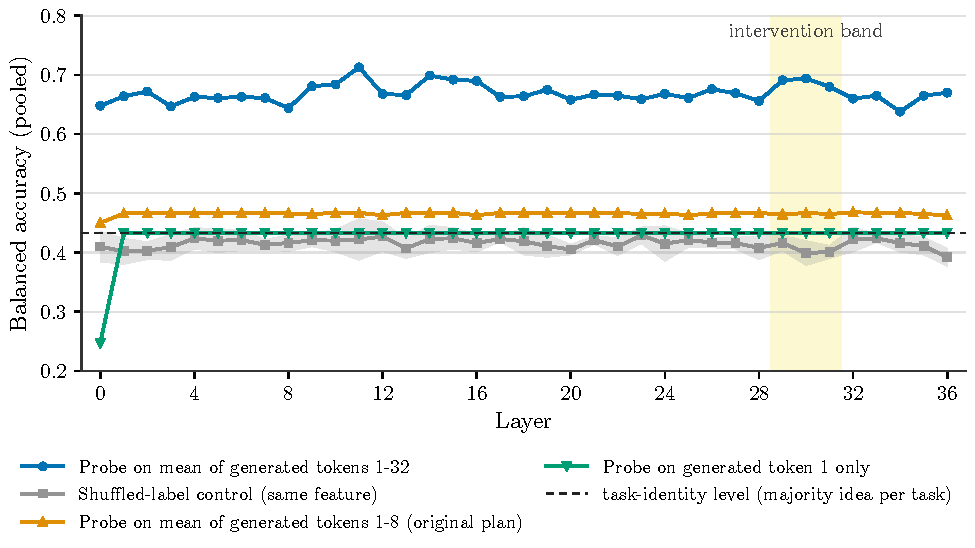
\includegraphics[width=\linewidth,height=0.85\textheight,keepaspectratio]{figures/fig_probe_v0.pdf}
\caption{Cross-validated (5-fold) balanced accuracy of multinomial probes for the realised idea class (BFS, DFS, Dijkstra, rare), against layer index, pooled over the open path-search and weighted shortest-path tasks (Qwen2.5-3B-Instruct, 300 baseline samples per task). Blue circles: probe on the mean residual over generated tokens 1--32. It reaches 0.64--0.71 at every layer, against 0.39--0.43 for the grey squares, the same feature with labels shuffled within each task (shaded band: $\pm$1\,SD over 5 permutations). The gap is 0.22--0.30 and does not rise with depth. Orange triangles: mean over tokens 1--8, the originally planned feature, which stays at 0.45--0.47. Green triangles: generated token 1 alone, which is 0.25 at layer 0 and 0.433 from layer 1 on. That is exactly the black dashed line, the balanced accuracy of predicting each task's majority idea, so the earliest tokens recover only which task is being solved. The yellow span marks layers 29--31, the band used for the steering interventions. [Source: artifact gen\_art\_experiment\_3, iteration 1.]}
\label{fig:fig_probe}
\end{figure}

\begingroup\scriptsize
\setlength{\tabcolsep}{2.0pt}
\begin{longtable}{@{}>{\raggedright\arraybackslash\hspace{0pt}}p{28.21pt}>{\raggedright\arraybackslash\hspace{0pt}}p{25.33pt}>{\raggedright\arraybackslash\hspace{0pt}}p{80.22pt}>{\raggedright\arraybackslash\hspace{0pt}}p{40.38pt}>{\raggedright\arraybackslash\hspace{0pt}}p{49.38pt}>{\raggedright\arraybackslash\hspace{0pt}}p{71.71pt}>{\raggedright\arraybackslash\hspace{0pt}}p{34.04pt}>{\raggedright\arraybackslash\hspace{0pt}}p{34.04pt}>{\raggedright\arraybackslash\hspace{0pt}}p{70.44pt}@{}}
\caption{Per-layer idea probes (5-fold CV, logistic regression with C chosen per layer). The gen1-only, gen8-only and mean(gen1..8) columns are the original plan's features; the mean(gen1..32) columns are the late-window feature actually used. [Source: artifact gen\_art\_experiment\_3, iteration 1.]}\label{tab:4}\\
\toprule
\textbf{layer} & \textbf{C} & \textbf{bal. acc. mean(gen1..32), pooled} & \textbf{open path search} & \textbf{weighted shortest path} & \textbf{shuffled-label pooled (mean \ensuremath{\pm} sd, 5 perms)} & \textbf{gen1 only} & \textbf{gen8 only} & \textbf{mean(gen1..8)} \\
\midrule
\endfirsthead
\multicolumn{9}{@{}l}{\emph{(continued)}}\\
\toprule
\textbf{layer} & \textbf{C} & \textbf{bal. acc. mean(gen1..32), pooled} & \textbf{open path search} & \textbf{weighted shortest path} & \textbf{shuffled-label pooled (mean \ensuremath{\pm} sd, 5 perms)} & \textbf{gen1 only} & \textbf{gen8 only} & \textbf{mean(gen1..8)} \\
\midrule
\endhead
\bottomrule
\endlastfoot
0 & 0.1 & 0.648 & 0.424 & 0.589 & 0.410 \ensuremath{\pm} 0.026 & 0.247 & 0.359 & 0.450 \\
1 & 1.0 & 0.664 & 0.440 & 0.602 & 0.402 \ensuremath{\pm} 0.022 & 0.433 & 0.468 & 0.466 \\
2 & 1.0 & 0.672 & 0.455 & 0.599 & 0.403 \ensuremath{\pm} 0.015 & 0.433 & 0.466 & 0.466 \\
3 & 1.0 & 0.647 & 0.420 & 0.597 & 0.409 \ensuremath{\pm} 0.022 & 0.433 & 0.463 & 0.467 \\
4 & 1.0 & 0.663 & 0.444 & 0.597 & 0.424 \ensuremath{\pm} 0.018 & 0.433 & 0.463 & 0.466 \\
5 & 1.0 & 0.661 & 0.438 & 0.591 & 0.420 \ensuremath{\pm} 0.020 & 0.433 & 0.463 & 0.467 \\
6 & 1.0 & 0.663 & 0.437 & 0.605 & 0.421 \ensuremath{\pm} 0.018 & 0.433 & 0.467 & 0.466 \\
7 & 0.1 & 0.661 & 0.440 & 0.594 & 0.413 \ensuremath{\pm} 0.009 & 0.433 & 0.468 & 0.467 \\
8 & 1.0 & 0.644 & 0.418 & 0.592 & 0.416 \ensuremath{\pm} 0.014 & 0.433 & 0.467 & 0.466 \\
9 & 0.01 & 0.681 & 0.464 & 0.589 & 0.421 \ensuremath{\pm} 0.011 & 0.433 & 0.466 & 0.465 \\
10 & 0.01 & 0.684 & 0.467 & 0.589 & 0.420 \ensuremath{\pm} 0.019 & 0.433 & 0.465 & 0.467 \\
11 & 1.0 & 0.713 & 0.500 & 0.606 & 0.422 \ensuremath{\pm} 0.035 & 0.433 & 0.463 & 0.467 \\
12 & 0.1 & 0.668 & 0.443 & 0.598 & 0.427 \ensuremath{\pm} 0.025 & 0.433 & 0.467 & 0.463 \\
13 & 1.0 & 0.666 & 0.443 & 0.600 & 0.407 \ensuremath{\pm} 0.017 & 0.433 & 0.468 & 0.467 \\
14 & 1.0 & 0.699 & 0.485 & 0.598 & 0.423 \ensuremath{\pm} 0.023 & 0.433 & 0.468 & 0.467 \\
15 & 0.01 & 0.692 & 0.475 & 0.594 & 0.424 \ensuremath{\pm} 0.018 & 0.433 & 0.468 & 0.467 \\
16 & 0.1 & 0.690 & 0.470 & 0.606 & 0.416 \ensuremath{\pm} 0.015 & 0.433 & 0.465 & 0.463 \\
17 & 0.01 & 0.663 & 0.439 & 0.600 & 0.423 \ensuremath{\pm} 0.005 & 0.433 & 0.467 & 0.467 \\
18 & 1.0 & 0.664 & 0.438 & 0.605 & 0.419 \ensuremath{\pm} 0.023 & 0.433 & 0.466 & 0.467 \\
19 & 1.0 & 0.675 & 0.458 & 0.602 & 0.411 \ensuremath{\pm} 0.019 & 0.433 & 0.467 & 0.467 \\
20 & 1.0 & 0.658 & 0.434 & 0.600 & 0.405 \ensuremath{\pm} 0.009 & 0.433 & 0.467 & 0.467 \\
21 & 0.01 & 0.667 & 0.446 & 0.589 & 0.421 \ensuremath{\pm} 0.007 & 0.433 & 0.465 & 0.467 \\
22 & 1.0 & 0.665 & 0.440 & 0.600 & 0.410 \ensuremath{\pm} 0.015 & 0.433 & 0.467 & 0.467 \\
23 & 0.01 & 0.659 & 0.439 & 0.595 & 0.429 \ensuremath{\pm} 0.014 & 0.433 & 0.468 & 0.465 \\
24 & 0.1 & 0.668 & 0.445 & 0.603 & 0.415 \ensuremath{\pm} 0.030 & 0.433 & 0.467 & 0.466 \\
25 & 1.0 & 0.661 & 0.437 & 0.605 & 0.421 \ensuremath{\pm} 0.012 & 0.433 & 0.468 & 0.463 \\
26 & 1.0 & 0.676 & 0.455 & 0.605 & 0.417 \ensuremath{\pm} 0.009 & 0.433 & 0.464 & 0.466 \\
27 & 0.1 & 0.669 & 0.447 & 0.600 & 0.416 \ensuremath{\pm} 0.010 & 0.433 & 0.463 & 0.466 \\
28 & 1.0 & 0.656 & 0.434 & 0.594 & 0.408 \ensuremath{\pm} 0.020 & 0.433 & 0.465 & 0.467 \\
29 & 1.0 & 0.691 & 0.477 & 0.598 & 0.416 \ensuremath{\pm} 0.013 & 0.433 & 0.464 & 0.464 \\
30 & 1.0 & 0.694 & 0.481 & 0.595 & 0.399 \ensuremath{\pm} 0.021 & 0.433 & 0.468 & 0.467 \\
31 & 1.0 & 0.680 & 0.460 & 0.601 & 0.401 \ensuremath{\pm} 0.011 & 0.433 & 0.466 & 0.465 \\
32 & 1.0 & 0.660 & 0.437 & 0.600 & 0.422 \ensuremath{\pm} 0.021 & 0.433 & 0.467 & 0.468 \\
33 & 0.1 & 0.665 & 0.442 & 0.603 & 0.424 \ensuremath{\pm} 0.007 & 0.433 & 0.468 & 0.467 \\
34 & 1.0 & 0.638 & 0.409 & 0.598 & 0.416 \ensuremath{\pm} 0.015 & 0.433 & 0.467 & 0.467 \\
35 & 0.1 & 0.665 & 0.442 & 0.603 & 0.411 \ensuremath{\pm} 0.015 & 0.433 & 0.468 & 0.465 \\
36 & 1.0 & 0.670 & 0.450 & 0.597 & 0.392 \ensuremath{\pm} 0.015 & 0.433 & 0.468 & 0.463 \\
\end{longtable}
\endgroup
What this settles for the hypothesis is limited but real. In this model and protocol, no linear readout at the prompt-final token or the first 8 generated tokens predicts the idea. The idea becomes decodable only once the 32-token window includes the explanatory preamble, which places the commitment token, if there is a single one, somewhere after token 8. Whether it precedes the first mention of the algorithm's name cannot be read from these data. Forking-path resampling, which would locate it per sample, belonged to the temperature arm and did not run.

\subsection{Building the intervention vectors, with offline checks}
All vectors were built from the baseline only, at layers 29 to 31. Three checks were run before any steered generation.

\emph{The two flattening directions are nearly orthogonal.} The probe-weight direction and the difference-in-means direction have cosine 0.16 to 0.23, so the two flattening variants are different interventions, not two estimates of one.

\begingroup\small
\setlength{\tabcolsep}{4.0pt}
\begin{longtable}{@{}>{\raggedright\arraybackslash\hspace{0pt}}p{97.72pt}>{\raggedright\arraybackslash\hspace{0pt}}p{217.01pt}>{\raggedright\arraybackslash\hspace{0pt}}p{131.02pt}@{}}
\caption{Cosine between the probe-weight and difference-in-means flattening directions. [Source: artifact gen\_art\_experiment\_3, iteration 1.]}\label{tab:5}\\
\toprule
\textbf{layer} & \textbf{cos(probe-weight dir., diff-in-means dir.) open path search} & \textbf{weighted shortest path} \\
\midrule
\endfirsthead
\multicolumn{3}{@{}l}{\emph{(continued)}}\\
\toprule
\textbf{layer} & \textbf{cos(probe-weight dir., diff-in-means dir.) open path search} & \textbf{weighted shortest path} \\
\midrule
\endhead
\bottomrule
\endlastfoot
layer 29 & 0.207 & 0.159 \\
layer 30 & 0.225 & 0.163 \\
layer 31 & 0.213 & 0.170 \\
\end{longtable}
\endgroup
\emph{LEACE [8] erases idea information offline; rank-1 projection nearly does.} On cached activations, a fresh probe for the menu label reaches a balanced accuracy of 0.58 to 0.61 on the open task and 0.88 to 0.89 on the weighted task before erasure. After LEACE it reaches 0.20 and 0.33 to 0.35 (chance is 0.33); after rank-1 projection, 0.32 to 0.34. The menu-centroid subspace is effectively one-dimensional: the second singular value of the centred centroid matrix is about 6 times smaller than the first on the open task and 56 to 61 times smaller on the weighted task.

\begingroup\footnotesize
\setlength{\tabcolsep}{3.0pt}
\begin{longtable}{@{}>{\raggedright\arraybackslash\hspace{0pt}}p{129.16pt}>{\raggedright\arraybackslash\hspace{0pt}}p{59.57pt}>{\raggedright\arraybackslash\hspace{0pt}}p{49.04pt}>{\raggedright\arraybackslash\hspace{0pt}}p{79.52pt}>{\raggedright\arraybackslash\hspace{0pt}}p{51.28pt}>{\raggedright\arraybackslash\hspace{0pt}}p{65.18pt}@{}}
\caption{Offline erasure check: balanced accuracy of a fresh 5-fold probe for the menu label (menu classes plus a pooled class for everything else) before and after erasure. [Source: artifact gen\_art\_experiment\_3, iteration 1.]}\label{tab:6}\\
\toprule
\textbf{task, layer} & \textbf{probe bal. acc. before} & \textbf{after LEACE} & \textbf{after rank-1 projection} & \textbf{chance} & \textbf{majority share} \\
\midrule
\endfirsthead
\multicolumn{6}{@{}l}{\emph{(continued)}}\\
\toprule
\textbf{task, layer} & \textbf{probe bal. acc. before} & \textbf{after LEACE} & \textbf{after rank-1 projection} & \textbf{chance} & \textbf{majority share} \\
\midrule
\endhead
\bottomrule
\endlastfoot
open path search, layer 29 & 0.607 & 0.198 & 0.334 & 0.333 & 0.683 \\
weighted shortest path, layer 29 & 0.888 & 0.334 & 0.325 & 0.333 & 0.750 \\
open path search, layer 30 & 0.582 & 0.199 & 0.337 & 0.333 & 0.683 \\
weighted shortest path, layer 30 & 0.884 & 0.352 & 0.323 & 0.333 & 0.750 \\
open path search, layer 31 & 0.577 & 0.198 & 0.339 & 0.333 & 0.683 \\
weighted shortest path, layer 31 & 0.893 & 0.332 & 0.323 & 0.333 & 0.750 \\
\end{longtable}
\endgroup
\begingroup\small
\setlength{\tabcolsep}{4.0pt}
\begin{longtable}{@{}>{\raggedright\arraybackslash\hspace{0pt}}p{241.58pt}>{\raggedright\arraybackslash\hspace{0pt}}p{102.64pt}>{\raggedright\arraybackslash\hspace{0pt}}p{101.52pt}@{}}
\caption{Singular values of the centred menu-centroid matrix (k = 2 menu classes, so the rank is at most 1). [Source: artifact gen\_art\_experiment\_3, iteration 1.]}\label{tab:7}\\
\toprule
\textbf{task, layer} & \textbf{singular value 1} & \textbf{singular value 2} \\
\midrule
\endfirsthead
\multicolumn{3}{@{}l}{\emph{(continued)}}\\
\toprule
\textbf{task, layer} & \textbf{singular value 1} & \textbf{singular value 2} \\
\midrule
\endhead
\bottomrule
\endlastfoot
open path search, layer 29 & 3.632 & 0.576 \\
weighted shortest path, layer 29 & 7.930 & 0.134 \\
open path search, layer 30 & 4.023 & 0.626 \\
weighted shortest path, layer 30 & 8.834 & 0.145 \\
open path search, layer 31 & 4.848 & 0.811 \\
weighted shortest path, layer 31 & 10.148 & 0.180 \\
\end{longtable}
\endgroup
\emph{The cross-task novelty direction transfers as a readout.} Extracted from sorting, substring search, primality testing, string compression and matrix multiplication prompts only, the direction separates novel-request from plain prompts on held-out path-search and weighted-path prompts with AUROC 1.0 at all three layers. Leave-one-task-out directions have cosine 0.92 to 0.98 with each held-out task's own difference vector. The direction is close to orthogonal to both flattening directions and to the erasure subspace (absolute cosines at most 0.095).

\begingroup\scriptsize
\setlength{\tabcolsep}{2.0pt}
\begin{longtable}{@{}>{\raggedright\arraybackslash\hspace{0pt}}p{24.74pt}>{\raggedright\arraybackslash\hspace{0pt}}p{34.67pt}>{\raggedright\arraybackslash\hspace{0pt}}p{41.68pt}>{\raggedright\arraybackslash\hspace{0pt}}p{41.68pt}>{\raggedright\arraybackslash\hspace{0pt}}p{50.46pt}>{\raggedright\arraybackslash\hspace{0pt}}p{28.52pt}>{\raggedright\arraybackslash\hspace{0pt}}p{29.77pt}>{\raggedright\arraybackslash\hspace{0pt}}p{37.83pt}>{\raggedright\arraybackslash\hspace{0pt}}p{45.57pt}>{\raggedright\arraybackslash\hspace{0pt}}p{45.51pt}>{\raggedright\arraybackslash\hspace{0pt}}p{45.33pt}@{}}
\caption{Cross-task novelty direction: transfer and overlap checks. [Source: artifact gen\_art\_experiment\_3, iteration 1.]}\label{tab:8}\\
\toprule
\textbf{layer} & \textbf{leave-one-task-out cosine: sorting} & \textbf{substring} & \textbf{primality} & \textbf{compression} & \textbf{matmul} & \textbf{held-out AUROC open path search} & \textbf{weighted shortest path} & \textbf{cos with probe-weight dir. (path / weighted)} & \textbf{cos with diff-in-means dir. (path / weighted)} & \textbf{cos with erasure subspace (path / weighted)} \\
\midrule
\endfirsthead
\multicolumn{11}{@{}l}{\emph{(continued)}}\\
\toprule
\textbf{layer} & \textbf{leave-one-task-out cosine: sorting} & \textbf{substring} & \textbf{primality} & \textbf{compression} & \textbf{matmul} & \textbf{held-out AUROC open path search} & \textbf{weighted shortest path} & \textbf{cos with probe-weight dir. (path / weighted)} & \textbf{cos with diff-in-means dir. (path / weighted)} & \textbf{cos with erasure subspace (path / weighted)} \\
\midrule
\endhead
\bottomrule
\endlastfoot
layer 29 & 0.941 & 0.978 & 0.956 & 0.934 & 0.966 & 1.0 & 1.0 & 0.037 / -0.027 & 0.008 / 0.093 & 0.009 / 0.095 \\
layer 30 & 0.943 & 0.977 & 0.956 & 0.925 & 0.966 & 1.0 & 1.0 & 0.027 / -0.013 & -0.021 / 0.082 & 0.024 / 0.088 \\
layer 31 & 0.946 & 0.978 & 0.952 & 0.919 & 0.964 & 1.0 & 1.0 & 0.021 / -0.028 & 0.011 / 0.038 & 0.039 / 0.039 \\
\end{longtable}
\endgroup
\subsection{Strength calibration}
Strengths for the three additive knobs were calibrated on the open task with n = 20 per point over a grid of 10 values. The lower bound is the largest grid value with pass at least 0.95x baseline, the upper bound the smallest larger value with pass at most 0.40x baseline, and five strengths are spaced geometrically between them. The calibration was frozen before the full run and reused for the weighted task and the random controls. The calibration rows already show what the full sweep confirms: both flattening directions convert the open task to DFS well before they break code (difference-in-means at \ensuremath{\alpha} = 0.2 gives DFS 19 of 20), and the probe-weight direction keeps pass near baseline up to \ensuremath{\alpha} = 0.75 only because its samples are almost all DFS.

\begingroup\footnotesize
\setlength{\tabcolsep}{3.0pt}
\begin{longtable}{@{}>{\raggedright\arraybackslash\hspace{0pt}}p{149.98pt}>{\raggedright\arraybackslash\hspace{0pt}}p{60.16pt}>{\raggedright\arraybackslash\hspace{0pt}}p{49.35pt}>{\raggedright\arraybackslash\hspace{0pt}}p{63.22pt}>{\raggedright\arraybackslash\hspace{0pt}}p{117.03pt}@{}}
\caption{Strength calibration on the open task (n = 20 per row). [Source: artifact gen\_art\_experiment\_3, iteration 1.]}\label{tab:9}\\
\toprule
\textbf{knob} & \textbf{strength \ensuremath{\alpha}} & \textbf{pass (n=20)} & \textbf{degenerate share} & \textbf{idea labels} \\
\midrule
\endfirsthead
\multicolumn{5}{@{}l}{\emph{(continued)}}\\
\toprule
\textbf{knob} & \textbf{strength \ensuremath{\alpha}} & \textbf{pass (n=20)} & \textbf{degenerate share} & \textbf{idea labels} \\
\midrule
\endhead
\bottomrule
\endlastfoot
probe-weight direction & 0.02 & 0.75 & 0.00 & DFS 4, BFS 15, Dijkstra 1 \\
probe-weight direction & 0.05 & 0.55 & 0.00 & DFS 8, BFS 11, A* 1 \\
probe-weight direction & 0.1 & 0.60 & 0.00 & DFS 12, A* 1, BFS 6, other 1 \\
probe-weight direction & 0.2 & 0.90 & 0.00 & DFS 14, BFS 5, other 1 \\
probe-weight direction & 0.35 & 0.85 & 0.00 & DFS 19, other 1 \\
probe-weight direction & 0.5 & 0.65 & 0.00 & DFS 20 \\
probe-weight direction & 0.75 & 0.70 & 0.00 & DFS 19, BFS 1 \\
probe-weight direction & 1.0 & 0.45 & 0.25 & DFS 14, syntax error 5, BFS 1 \\
probe-weight direction & 1.5 & 0.05 & 0.70 & other 3, syntax error 14, DFS 3 \\
probe-weight direction & 2.0 & 0.20 & 0.85 & no code 14, DFS 4, syntax error 1, BFS 1 \\
probe-weight direction & \textbf{chosen} & \ensuremath{\alpha}\_lo = 0.75, \ensuremath{\alpha}\_hi = 1.5 &  & 0.75, 0.892, 1.06, 1.26, 1.5 \\
difference-in-means direction & 0.02 & 0.65 & 0.00 & DFS 9, BFS 10, A* 1 \\
difference-in-means direction & 0.05 & 0.75 & 0.00 & DFS 13, BFS 6, other 1 \\
difference-in-means direction & 0.1 & 0.65 & 0.00 & DFS 15, BFS 5 \\
difference-in-means direction & 0.2 & 0.60 & 0.00 & DFS 19, BFS 1 \\
difference-in-means direction & 0.35 & 0.40 & 0.00 & DFS 17, BFS 2, other 1 \\
difference-in-means direction & 0.5 & 0.65 & 0.00 & DFS 19, BFS 1 \\
difference-in-means direction & 0.75 & 0.30 & 0.15 & syntax error 1, other 1, DFS 16, BFS 2 \\
difference-in-means direction & 1.0 & 0.00 & 0.95 & no code 10, syntax error 9, DFS 1 \\
difference-in-means direction & 1.5 & 0.10 & 0.80 & DFS 1, no code 16, BFS 2, other 1 \\
difference-in-means direction & 2.0 & 0.00 & 0.95 & no code 19, other 1 \\
difference-in-means direction & \textbf{chosen} & \ensuremath{\alpha}\_lo = 0.05, \ensuremath{\alpha}\_hi = 1.0 &  & 0.05, 0.106, 0.224, 0.473, 1.0 \\
novelty direction & 0.02 & 0.55 & 0.00 & DFS 3, BFS 16, A* 1 \\
novelty direction & 0.05 & 0.65 & 0.00 & DFS 5, BFS 14, A* 1 \\
novelty direction & 0.1 & 0.80 & 0.00 & DFS 7, BFS 12, A* 1 \\
novelty direction & 0.2 & 0.85 & 0.00 & DFS 10, BFS 10 \\
novelty direction & 0.35 & 0.60 & 0.00 & A* 2, BFS 9, DFS 7, other 1, Dijkstra 1 \\
novelty direction & 0.5 & 0.45 & 0.00 & Dijkstra 2, DFS 11, BFS 4, A* 3 \\
novelty direction & 0.75 & 0.60 & 0.00 & BFS 11, Dijkstra 1, DFS 7, greedy best-first search 1 \\
novelty direction & 1.0 & 0.40 & 0.00 & DFS 9, BFS 8, A* 1, Dijkstra 2 \\
novelty direction & 1.5 & 0.60 & 0.05 & BFS 12, DFS 4, Dijkstra 2, no code 1, A* 1 \\
novelty direction & 2.0 & 0.65 & 0.05 & DFS 6, BFS 12, no code 1, Dijkstra 1 \\
novelty direction & \textbf{chosen} & \ensuremath{\alpha}\_lo = 0.2, \ensuremath{\alpha}\_hi = 2.0 &  & 0.2, 0.356, 0.632, 1.12, 2.0 \\
\end{longtable}
\endgroup
\subsection{Main sweep: practitioner knobs}
The sweep used seeds 0..149 for every method setting and seeds 0..74 for random controls (n = 150 and 75 per task). Table 10 holds the knobs a practitioner would reach for (\texttt{gen\_\allowbreak{}art\_\allowbreak{}experiment\_\allowbreak{}3}). Three results stand out.

First, temperature buys almost no idea diversity before it breaks the code. Between T = 0.7 and T = 1.0 idea entropy rises from 1.175 to 1.278 bits on the open task and from 0.916 to 1.165 on the weighted task, while the weighted-task pass rate falls from 0.380 to 0.233. T = 1.0 misses pooled eligibility by 0.006 (0.423 against 0.429), so the best eligible temperature is T = 0.7 itself. At T = 1.3 a quarter to a third of outputs are syntax errors, at T = 1.6 almost all are, and at T = 2.0 one output in 300 contains a parseable program. Top-k = 10 at T = 1.6 keeps most outputs parseable but the pass rate is still 0.227 and 0.040. Across all temperatures the same two menu ideas dominate the outputs that parse; no temperature introduced a third idea class above 5\% of samples.

\begin{figure}[!htbp]
\centering
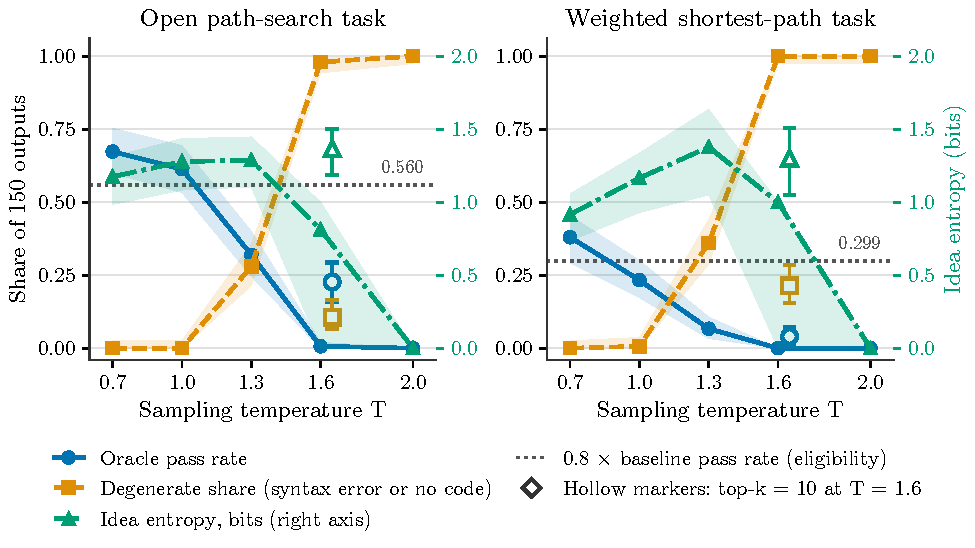
\includegraphics[width=\linewidth,height=0.85\textheight,keepaspectratio]{figures/fig_temp_v0.pdf}
\caption{Temperature sweep in the influence arm (Qwen2.5-3B-Instruct, $n = 150$ generations per point; $T = 0.7$ is the baseline draw). Left: open path-search task; right: weighted shortest-path task. Blue solid line with circles: oracle pass rate; amber dashed line with squares: degenerate share (syntax error or no code); both on the left axis as a share of the 150 outputs. Green dash-dot line with triangles: idea entropy in bits (right axis). Shaded bands are 95\% confidence intervals (bootstrap for pass rate and entropy, Wilson for degenerate share). Hollow markers, drawn just right of $T = 1.6$, show top-$k = 10$ sampling at $T = 1.6$ with 95\% CIs. The grey dotted line is the eligibility threshold, $0.8\times$ the $n = 300$ baseline pass rate (0.560 and 0.299). Pass rate falls and degeneration rises from $T = 1.0$ on, while idea entropy rises by at most 0.46 bits (weighted task, $T = 1.3$) before collapsing; at $T = 2.0$ entropy is 0 because no output (open task) or one output in 150 (weighted task) contains a classifiable program. Top-$k = 10$ at $T = 1.6$ keeps most code parseable (degenerate share 0.11 and 0.21) but not correct (pass 0.23 and 0.04). No temperature above the baseline keeps 80\% of baseline pass rate on the pooled tasks, so $T = 0.7$ is the best eligible temperature. [Source: artifact gen\_art\_experiment\_3, iteration 1.]}
\label{fig:fig_temp}
\end{figure}

Second, the top-3 ban is largely ignored. On the open task, 142 of 150 programs (0.947) still implement a banned idea, and the ban only evens BFS and DFS out (70/70), which raises entropy from 1.175 to 1.404 bits. On the weighted task 131 of 150 (0.873) still implement Dijkstra, BFS or SPFA; the ban shifts mass from Dijkstra to BFS (from 111/37 to 62/66), which raises entropy to 1.779 bits and drops the pass rate from 0.380 to 0.153, because BFS-style programs fail on weighted graphs. Small amounts of Bellman-Ford (7) and Floyd-Warshall (3) appear. The entropy gain from the ban on the weighted task is mostly a move toward the incorrect menu idea. Non-compliance with negative instructions is a known failure: naming a forbidden item can prime it [5]. The artifact also rendered a PCA view of layer-30 window activations with per-idea centroids for the baseline, the ban and the best projection setting. It is not reproduced here, because its coordinates were not written to the results files, and it is not the planned manifold analysis, which belonged to the ban arm.

\begin{correction}\textbf{Correction (iteration 2).} The statement that the ban is largely ignored holds only for this prompt: the contract prompt with a list-style prohibition (\texttt{Do\ not\ use\ any\ of\ the\ following\ algorithms:\allowbreak{}\ ...}). On the bare prompt with the short wording \texttt{Do\ not\ use\ X,\ Y\ or\ Z.}, the same model complies far more often: 1 of 100 programs still uses BFS when BFS is banned on the open task, 29 of 100 still use a banned idea under the top-3 ban and 38 of 100 under the top-5 ban; on the sorting task 0 of 100 under the top-3 ban; on the weighted task 12, 46 and 61 of 100 for the top-1, top-3 and top-5 bans (Section 2.4). The contract and the wording are confounded, so the difference is unexplained.\end{correction}
Third, the novelty prompts split. The new-algorithm prompt leaves the pooled numbers almost unchanged (pass 0.553, entropy 1.053) but moves the two tasks in opposite directions: more DFS, A* and Dijkstra on the open task (entropy 1.533), and more Dijkstra on the weighted task (137 of 150; entropy 0.573, pass 0.547, the highest weighted-task pass rate in the sweep; the held-out re-draw gives 0.580). The 2000-word novelty prompt raises entropy to 2.205 bits pooled but collapses the pass rate to 0.083, with 39 and 64 syntax errors. Generate-then-select gives the highest entropy of all (2.561 pooled; 9 idea classes on each task) at pass 0.263: listing approaches first does put A*, bidirectional, IDDFS, Bellman-Ford and Floyd-Warshall into the outputs, but these implementations fail the oracle more often.

\begingroup\tiny
\setlength{\tabcolsep}{1.5pt}
\begin{longtable}{@{}>{\raggedright\arraybackslash\hspace{0pt}}p{70.65pt}>{\raggedright\arraybackslash\hspace{0pt}}p{16.31pt}>{\raggedright\arraybackslash\hspace{0pt}}p{20.60pt}>{\raggedright\arraybackslash\hspace{0pt}}p{27.46pt}>{\raggedright\arraybackslash\hspace{0pt}}p{70.63pt}>{\raggedright\arraybackslash\hspace{0pt}}p{33.75pt}>{\raggedright\arraybackslash\hspace{0pt}}p{34.12pt}>{\raggedright\arraybackslash\hspace{0pt}}p{78.39pt}>{\raggedright\arraybackslash\hspace{0pt}}p{23.89pt}>{\raggedright\arraybackslash\hspace{0pt}}p{27.50pt}>{\raggedright\arraybackslash\hspace{0pt}}p{33.44pt}@{}}
\caption{Practitioner knobs and noise-floor rerun (sweep seeds 0..149). [Source: artifact gen\_art\_experiment\_3, iteration 1.]}\label{tab:10}\\
\toprule
\textbf{setting} & \textbf{n per task} & \textbf{path: pass} & \textbf{path: idea entropy} & \textbf{path: idea labels} & \textbf{weighted: pass} & \textbf{weighted: idea entropy} & \textbf{weighted: idea labels} & \textbf{pooled pass} & \textbf{pooled idea entropy} & \textbf{eligible (path / weighted / pooled)} \\
\midrule
\endfirsthead
\multicolumn{11}{@{}l}{\emph{(continued)}}\\
\toprule
\textbf{setting} & \textbf{n per task} & \textbf{path: pass} & \textbf{path: idea entropy} & \textbf{path: idea labels} & \textbf{weighted: pass} & \textbf{weighted: idea entropy} & \textbf{weighted: idea labels} & \textbf{pooled pass} & \textbf{pooled idea entropy} & \textbf{eligible (path / weighted / pooled)} \\
\midrule
\endhead
\bottomrule
\endlastfoot
baseline T=0.7 & 150 & 0.673 & 1.175 & BFS 98, DFS 44, other 7, Dijkstra 1 & 0.380 & 0.916 & Dijkstra 111, BFS 37, other 1, SPFA 1 & 0.527 & 1.045 & y / y / y \\
baseline rerun (noise floor) & 150 & 0.673 & 1.133 & BFS 95, DFS 50, other 4, Dijkstra 1 & 0.413 & 0.891 & Dijkstra 109, BFS 40, SPFA 1 & 0.543 & 1.012 & y / y / y \\
temperature 1.0 & 150 & 0.613 & 1.278 & BFS 82, DFS 61, other 3, Dijkstra 3, A* 1 & 0.233 & 1.165 & Dijkstra 105, BFS 35, other 6, DFS 2, greedy best-first search 1, syntax error 1 & 0.423 & 1.222 & y / n / n \\
temperature 1.3 & 150 & 0.320 & 1.288 & BFS 52, DFS 51, syntax error 41, other 5, Dijkstra 1 & 0.067 & 1.377 & Dijkstra 73, syntax error 48, BFS 15, other 7, DFS 4, greedy best-first search 2, A* 1 & 0.193 & 1.333 & n / n / n \\
temperature 1.6 & 150 & 0.007 & 0.811 & syntax error 139, no code 7, BFS 3, other 1 & 0.000 & 1.000 & syntax error 134, no code 14, Dijkstra 1, other 1 & 0.003 & 0.906 & n / n / n \\
temperature 1.6, top-k 10 & 150 & 0.227 & 1.366 & BFS 71, DFS 56, syntax error 13, other 6, Dijkstra 4 & 0.040 & 1.301 & Dijkstra 84, syntax error 27, BFS 26, other 7, DFS 4, greedy best-first search 1, no code 1 & 0.133 & 1.333 & n / n / n \\
temperature 2.0 & 150 & 0.000 & 0.000 & syntax error 78, no code 72 & 0.000 & 0.000 & no code 78, syntax error 71, other 1 & 0.000 & 0.000 & n / n / n \\
new-algorithm prompt & 150 & 0.560 & 1.533 & BFS 75, DFS 61, A* 6, Dijkstra 4, other 2, bidirectional 1, iterative deepening 1 & 0.547 & 0.573 & Dijkstra 137, BFS 8, Bellman-Ford 2, Floyd-Warshall 1, SPFA 1, other 1 & 0.553 & 1.053 & y / y / y \\
2000-word novelty prompt & 150 & 0.113 & 1.881 & DFS 65, syntax error 39, BFS 24, other 6, bidirectional 4, Dijkstra 4, greedy best-first search 2, random walk 2, iterative deepening 2, no code 1, A* 1 & 0.053 & 2.528 & syntax error 64, Dijkstra 37, BFS 17, other 7, greedy best-first search 5, DFS 5, bidirectional 4, random walk 3, Bellman-Ford 3, no code 2, Floyd-Warshall 2, A* 1 & 0.083 & 2.205 & n / n / n \\
top-3 ban & 150 & 0.707 & 1.404 & DFS 70, BFS 70, other 5, Dijkstra 2, A* 2, greedy best-first search 1 & 0.153 & 1.779 & BFS 66, Dijkstra 62, Bellman-Ford 7, other 6, DFS 3, Floyd-Warshall 3, SPFA 3 & 0.430 & 1.591 & y / n / y \\
generate-then-select & 150 & 0.353 & 2.549 & Dijkstra 45, DFS 40, BFS 26, bidirectional 10, A* 10, iterative deepening 6, other 6, syntax error 3, random walk 2, greedy best-first search 2 & 0.173 & 2.574 & Dijkstra 58, A* 21, BFS 19, Floyd-Warshall 13, Bellman-Ford 13, bidirectional 9, syntax error 7, greedy best-first search 5, DFS 3, other 2 & 0.263 & 2.561 & n / n / n \\
\end{longtable}
\endgroup
Table 11 lists what the generate-then-select pipeline chose in stage 1. The picked names are far more varied than what the model writes unprompted; on the weighted task they include the Johnson, Kruskal and Prim algorithms (the last two are minimum-spanning-tree methods, not shortest-path methods), A* search and Bellman-Ford.

\begingroup\small
\setlength{\tabcolsep}{4.0pt}
\begin{longtable}{@{}>{\raggedright\arraybackslash\hspace{0pt}}p{54.69pt}>{\raggedright\arraybackslash\hspace{0pt}}p{47.32pt}>{\raggedright\arraybackslash\hspace{0pt}}p{41.98pt}>{\raggedright\arraybackslash\hspace{0pt}}p{293.77pt}@{}}
\caption{Generate-then-select, stage 1: items picked by the seeded RNG from the 10-item lists the model wrote itself (possessive apostrophes dropped from item names). [Source: artifact gen\_art\_experiment\_3, iteration 1.]}\label{tab:11}\\
\toprule
\textbf{task} & \textbf{stage-1 lists parsed} & \textbf{mean items listed} & \textbf{15 most frequent picked items (count)} \\
\midrule
\endfirsthead
\multicolumn{4}{@{}l}{\emph{(continued)}}\\
\toprule
\textbf{task} & \textbf{stage-1 lists parsed} & \textbf{mean items listed} & \textbf{15 most frequent picked items (count)} \\
\midrule
\endhead
\bottomrule
\endlastfoot
open path search & 150/150 & 9.99 & Bidirectional Search (15); Depth-First Search (14); Dijkstra Algorithm (11); Uniform Cost Search (11); Breadth-First Search (10); Depth-First Search (DFS) (9); A* Search Algorithm (8); Greedy Best-First Search (8); Hill Climbing Search (6); Best-First Search (3); A* Search (3); Depth-First Search with Iterative Deepening (3); Wavefront Search (2); Bi-directional Search (2); Iterative Deepening Search (2) \\
weighted shortest path & 150/150 & 9.97 & A* Search Algorithm (19); Bellman-Ford Algorithm (14); Dijkstra Algorithm (11); Floyd-Warshall Algorithm (11); Bidirectional Search (9); Johnson Algorithm (9); Breadth-First Search (BFS) with Relaxation (4); Kruskal Algorithm (3); Breadth-First Search (BFS) with relaxation (3); A* Search (2); Breadth-First Search (with relaxation) (2); Bi-directional Search (2); Johnson algorithm (2); Prim Minimum Spanning Tree (MST) Algorithm (2); Kruskal MST Approach for Shortest Path (via MST) (1) \\
\end{longtable}
\endgroup
\subsection{Main sweep: internal knobs}
\textbf{Flattening directions.} Neither flattening direction flattens (\texttt{gen\_\allowbreak{}art\_\allowbreak{}experiment\_\allowbreak{}3}). The difference-in-means direction at \ensuremath{\alpha} = 0.224 turns the open task into DFS on 145 of 150 samples (baseline BFS 98, DFS 44) at an unchanged pass rate (0.680 against 0.673); at \ensuremath{\alpha} = 0.106 it already gives DFS 126. Idea entropy therefore falls, to 0.235 bits. The probe-weight direction does the same at \ensuremath{\alpha} = 0.75 (DFS 148 of 150) at a lower pass rate (0.580). On the weighted task the same directions push Dijkstra toward BFS: at \ensuremath{\alpha} = 0.224 the split is 77/60 against 111/37 at baseline, entropy rises to 1.444 bits, and the pass rate falls to 0.287 because more programs are BFS. With only two menu ideas, a direction that points from the mode toward the mean of the menu overshoots the uniform point and selects the minority idea. At the top strengths both directions destroy the output: the difference-in-means direction at \ensuremath{\alpha} = 1.0 leaves 148 of 150 open-task samples with no code or a syntax error, the probe-weight direction at \ensuremath{\alpha} = 1.5 leaves 125.

\begingroup\scriptsize
\setlength{\tabcolsep}{2.0pt}
\begin{longtable}{@{}>{\raggedright\arraybackslash\hspace{0pt}}p{79.41pt}>{\raggedright\arraybackslash\hspace{0pt}}p{18.59pt}>{\raggedright\arraybackslash\hspace{0pt}}p{23.06pt}>{\raggedright\arraybackslash\hspace{0pt}}p{31.74pt}>{\raggedright\arraybackslash\hspace{0pt}}p{35.36pt}>{\raggedright\arraybackslash\hspace{0pt}}p{40.36pt}>{\raggedright\arraybackslash\hspace{0pt}}p{40.40pt}>{\raggedright\arraybackslash\hspace{0pt}}p{61.30pt}>{\raggedright\arraybackslash\hspace{0pt}}p{27.38pt}>{\raggedright\arraybackslash\hspace{0pt}}p{31.74pt}>{\raggedright\arraybackslash\hspace{0pt}}p{36.42pt}@{}}
\caption{Flattening directions (rows marked post hoc are excluded from survival). [Source: artifact gen\_art\_experiment\_3, iteration 1.]}\label{tab:12}\\
\toprule
\textbf{setting} & \textbf{n per task} & \textbf{path: pass} & \textbf{path: idea entropy} & \textbf{path: idea labels} & \textbf{weighted: pass} & \textbf{weighted: idea entropy} & \textbf{weighted: idea labels} & \textbf{pooled pass} & \textbf{pooled idea entropy} & \textbf{eligible (path / weighted / pooled)} \\
\midrule
\endfirsthead
\multicolumn{11}{@{}l}{\emph{(continued)}}\\
\toprule
\textbf{setting} & \textbf{n per task} & \textbf{path: pass} & \textbf{path: idea entropy} & \textbf{path: idea labels} & \textbf{weighted: pass} & \textbf{weighted: idea entropy} & \textbf{weighted: idea labels} & \textbf{pooled pass} & \textbf{pooled idea entropy} & \textbf{eligible (path / weighted / pooled)} \\
\midrule
\endhead
\bottomrule
\endlastfoot
probe-weight direction \ensuremath{\alpha}=0.75 & 150 & 0.580 & 0.102 & DFS 148, BFS 2 & 0.173 & 1.543 & BFS 88, Dijkstra 42, DFS 11, SPFA 4, other 3, syntax error 1, bidirectional 1 & 0.377 & 0.823 & y / n / n \\
probe-weight direction \ensuremath{\alpha}=0.892 & 150 & 0.387 & 0.323 & DFS 129, syntax error 14, BFS 6, other 1 & 0.087 & 1.522 & BFS 76, Dijkstra 44, DFS 18, syntax error 8, other 2, no code 1, SPFA 1 & 0.237 & 0.922 & n / n / n \\
probe-weight direction \ensuremath{\alpha}=1.06 & 150 & 0.247 & 0.806 & DFS 81, syntax error 54, BFS 10, other 4, Dijkstra 1 & 0.127 & 1.603 & BFS 60, Dijkstra 45, syntax error 19, DFS 16, no code 6, other 3, Floyd-Warshall 1 & 0.187 & 1.205 & n / n / n \\
probe-weight direction \ensuremath{\alpha}=1.26 & 150 & 0.020 & 0.994 & syntax error 117, DFS 18, other 15 & 0.200 & 1.410 & Dijkstra 71, BFS 28, no code 23, syntax error 17, DFS 5, other 4, bidirectional 1, Bellman-Ford 1 & 0.110 & 1.202 & n / n / n \\
probe-weight direction \ensuremath{\alpha}=1.5 & 150 & 0.007 & 0.943 & syntax error 121, other 16, DFS 9, no code 4 & 0.140 & 0.808 & no code 64, Dijkstra 62, syntax error 12, BFS 9, other 2, DFS 1 & 0.073 & 0.875 & n / n / n \\
difference-in-means direction \ensuremath{\alpha}=0.05 & 150 & 0.727 & 1.149 & DFS 87, BFS 58, other 5 & 0.420 & 0.972 & Dijkstra 106, BFS 40, other 3, syntax error 1 & 0.573 & 1.061 & y / y / y \\
difference-in-means direction \ensuremath{\alpha}=0.106 & 150 & 0.727 & 0.714 & DFS 126, BFS 22, other 1, A* 1 & 0.360 & 1.192 & Dijkstra 94, BFS 49, other 3, Bellman-Ford 2, syntax error 1, SPFA 1 & 0.543 & 0.953 & y / y / y \\
difference-in-means direction \ensuremath{\alpha}=0.224 & 150 & 0.680 & 0.235 & DFS 145, BFS 4, other 1 & 0.287 & 1.444 & Dijkstra 77, BFS 60, SPFA 6, other 4, bidirectional 1, syntax error 1, DFS 1 & 0.483 & 0.840 & y / n / y \\
difference-in-means direction \ensuremath{\alpha}=0.473 & 150 & 0.580 & 0.450 & DFS 138, BFS 7, other 4, syntax error 1 & 0.313 & 1.459 & Dijkstra 80, BFS 52, other 6, syntax error 4, DFS 3, no code 2, Floyd-Warshall 1, Bellman-Ford 1, SPFA 1 & 0.447 & 0.954 & y / y / y \\
difference-in-means direction \ensuremath{\alpha}=1 & 150 & 0.000 & 1.000 & no code 79, syntax error 69, DFS 1, other 1 & 0.033 & 1.141 & no code 110, syntax error 20, Dijkstra 13, BFS 6, other 1 & 0.017 & 1.071 & n / n / n \\
probe-weight direction \ensuremath{\alpha}=0.1 (post hoc) & 150 & 0.633 & 1.158 & DFS 83, BFS 62, other 3, A* 1, syntax error 1 & 0.247 & 1.152 & Dijkstra 86, BFS 58, other 5, syntax error 1 & 0.440 & 1.155 & y / n / y \\
probe-weight direction \ensuremath{\alpha}=0.2 (post hoc) & 150 & 0.733 & 1.046 & DFS 100, BFS 47, other 2, Dijkstra 1 & 0.287 & 1.223 & Dijkstra 78, BFS 66, other 5, SPFA 1 & 0.510 & 1.135 & y / n / y \\
probe-weight direction \ensuremath{\alpha}=0.35 (post hoc) & 150 & 0.807 & 0.415 & DFS 140, BFS 8, other 1, Dijkstra 1 & 0.313 & 1.340 & BFS 73, Dijkstra 69, SPFA 4, other 2, bidirectional 1, Bellman-Ford 1 & 0.560 & 0.877 & y / y / y \\
probe-weight direction \ensuremath{\alpha}=0.5 (post hoc) & 150 & 0.753 & 0.160 & DFS 147, BFS 2, Dijkstra 1 & 0.220 & 1.352 & BFS 74, Dijkstra 67, SPFA 5, DFS 2, other 2 & 0.487 & 0.756 & y / n / y \\
difference-in-means direction \ensuremath{\alpha}=0.075 (post hoc) & 150 & 0.740 & 0.978 & DFS 106, BFS 41, other 3 & 0.380 & 1.100 & Dijkstra 102, BFS 42, other 3, syntax error 1, DFS 1, bidirectional 1 & 0.560 & 1.039 & y / y / y \\
\end{longtable}
\endgroup
\begin{figure}[!htbp]
\centering
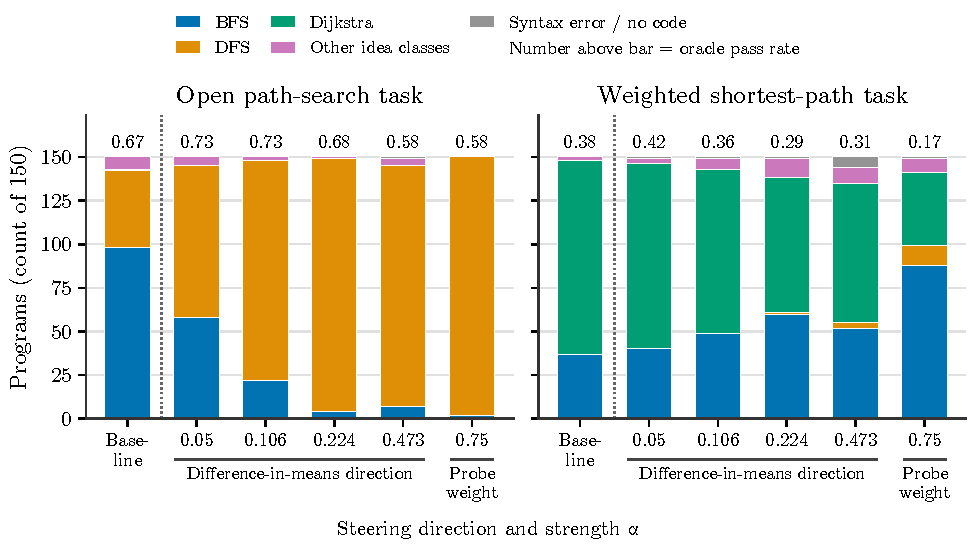
\includegraphics[width=\linewidth,height=0.85\textheight,keepaspectratio]{figures/fig_select_v0.pdf}
\caption{Idea composition of Qwen2.5-3B-Instruct's programs under the two `flattening' steering directions (added at layers 29--31 over the prompt-final token and the first 64 generated tokens; $n=150$ programs per bar). Left: open path-search task; right: weighted shortest-path task. Each stacked bar counts programs by idea class: BFS (blue), DFS (orange), Dijkstra (green), other idea classes (violet), syntax error or no code (grey). Bars show the unsteered baseline, the difference-in-means direction at $\alpha \in \{0.05, 0.106, 0.224, 0.473\}$ and the probe-weight direction at $\alpha=0.75$. The number above each bar is the oracle pass rate (all 50 fixed test graphs passed). Neither direction evens out the two menu ideas. Each one instead selects the baseline's minority idea. On the open task, DFS rises from 44 to 145 of 150 programs at difference-in-means $\alpha=0.224$ (148 under the probe direction) while the pass rate stays at 0.58--0.73 (baseline 0.67). On the weighted task, mass moves from Dijkstra to BFS (BFS 37 $\rightarrow$ 88 under the probe direction), where BFS-style programs rarely pass the oracle, and the pass rate falls from 0.38 to as low as 0.17. [Source: artifact gen\_art\_experiment\_3, iteration 1.]}
\label{fig:fig_select}
\end{figure}

\textbf{Menu erasure.} Rank-1 projection and LEACE leave the open-task distribution close to baseline and the weighted task more Dijkstra-heavy, at pass rates near baseline. LEACE at a = 1.0 gives open-task BFS 117 and weighted-task Dijkstra 127; rank-1 projection at a = 0.25 evens the open task (DFS 75, BFS 73) and raises weighted-task BFS to 47. No erasure setting produced a single passing program outside the known classes that the judge accepted as novel. Rank-1 projection at a = 0.5 and above produced 17 to 23 syntax errors on the open task.

\begingroup\scriptsize
\setlength{\tabcolsep}{2.0pt}
\begin{longtable}{@{}>{\raggedright\arraybackslash\hspace{0pt}}p{46.03pt}>{\raggedright\arraybackslash\hspace{0pt}}p{19.50pt}>{\raggedright\arraybackslash\hspace{0pt}}p{24.28pt}>{\raggedright\arraybackslash\hspace{0pt}}p{33.22pt}>{\raggedright\arraybackslash\hspace{0pt}}p{49.70pt}>{\raggedright\arraybackslash\hspace{0pt}}p{41.71pt}>{\raggedright\arraybackslash\hspace{0pt}}p{42.01pt}>{\raggedright\arraybackslash\hspace{0pt}}p{68.37pt}>{\raggedright\arraybackslash\hspace{0pt}}p{28.64pt}>{\raggedright\arraybackslash\hspace{0pt}}p{33.26pt}>{\raggedright\arraybackslash\hspace{0pt}}p{39.02pt}@{}}
\caption{Menu erasure. [Source: artifact gen\_art\_experiment\_3, iteration 1.]}\label{tab:13}\\
\toprule
\textbf{setting} & \textbf{n per task} & \textbf{path: pass} & \textbf{path: idea entropy} & \textbf{path: idea labels} & \textbf{weighted: pass} & \textbf{weighted: idea entropy} & \textbf{weighted: idea labels} & \textbf{pooled pass} & \textbf{pooled idea entropy} & \textbf{eligible (path / weighted / pooled)} \\
\midrule
\endfirsthead
\multicolumn{11}{@{}l}{\emph{(continued)}}\\
\toprule
\textbf{setting} & \textbf{n per task} & \textbf{path: pass} & \textbf{path: idea entropy} & \textbf{path: idea labels} & \textbf{weighted: pass} & \textbf{weighted: idea entropy} & \textbf{weighted: idea labels} & \textbf{pooled pass} & \textbf{pooled idea entropy} & \textbf{eligible (path / weighted / pooled)} \\
\midrule
\endhead
\bottomrule
\endlastfoot
rank-1 projection a=0.25 & 150 & 0.720 & 1.089 & DFS 75, BFS 73, other 2 & 0.380 & 1.027 & Dijkstra 100, BFS 47, other 3 & 0.550 & 1.058 & y / y / y \\
rank-1 projection a=0.5 & 150 & 0.640 & 0.983 & DFS 76, BFS 56, syntax error 18 & 0.347 & 0.958 & Dijkstra 101, BFS 48, DFS 1 & 0.493 & 0.971 & y / y / y \\
rank-1 projection a=0.75 & 150 & 0.627 & 1.086 & DFS 74, BFS 57, syntax error 17, other 2 & 0.233 & 1.117 & Dijkstra 96, BFS 49, other 2, SPFA 1, Bellman-Ford 1, syntax error 1 & 0.430 & 1.101 & y / n / y \\
rank-1 projection a=1 & 150 & 0.607 & 0.976 & DFS 75, BFS 52, syntax error 23 & 0.340 & 1.113 & Dijkstra 101, BFS 43, other 2, Bellman-Ford 2, syntax error 1, DFS 1 & 0.473 & 1.045 & y / y / y \\
LEACE erasure a=0.5 & 150 & 0.740 & 1.079 & BFS 100, DFS 46, other 2, Dijkstra 2 & 0.293 & 0.792 & Dijkstra 122, BFS 24, bidirectional 2, DFS 1, syntax error 1 & 0.517 & 0.936 & y / n / y \\
LEACE erasure a=1 & 150 & 0.673 & 1.072 & BFS 117, DFS 23, A* 5, other 2, Dijkstra 2, greedy best-first search 1 & 0.387 & 0.635 & Dijkstra 127, BFS 17, syntax error 4, Floyd-Warshall 1, DFS 1 & 0.530 & 0.853 & y / y / y \\
\end{longtable}
\endgroup
\textbf{Cross-task novelty direction.} This is the internal knob with the clearest effect on diversity. At \ensuremath{\alpha} = 0.356 the open task shows 7 idea classes (DFS 76, BFS 51, A* 9, Dijkstra 6, other 5, greedy best-first 2, bidirectional 1) and entropy 1.750 bits, at pass 0.560, just at the per-task eligibility line. The weighted task barely moves (entropy 0.984). At \ensuremath{\alpha} = 2.0 about 15\% of outputs contain no code.

\begingroup\scriptsize
\setlength{\tabcolsep}{2.0pt}
\begin{longtable}{@{}>{\raggedright\arraybackslash\hspace{0pt}}p{41.08pt}>{\raggedright\arraybackslash\hspace{0pt}}p{19.24pt}>{\raggedright\arraybackslash\hspace{0pt}}p{23.90pt}>{\raggedright\arraybackslash\hspace{0pt}}p{32.80pt}>{\raggedright\arraybackslash\hspace{0pt}}p{68.05pt}>{\raggedright\arraybackslash\hspace{0pt}}p{41.31pt}>{\raggedright\arraybackslash\hspace{0pt}}p{41.57pt}>{\raggedright\arraybackslash\hspace{0pt}}p{58.41pt}>{\raggedright\arraybackslash\hspace{0pt}}p{28.25pt}>{\raggedright\arraybackslash\hspace{0pt}}p{32.84pt}>{\raggedright\arraybackslash\hspace{0pt}}p{38.29pt}@{}}
\caption{Cross-task novelty direction. [Source: artifact gen\_art\_experiment\_3, iteration 1.]}\label{tab:14}\\
\toprule
\textbf{setting} & \textbf{n per task} & \textbf{path: pass} & \textbf{path: idea entropy} & \textbf{path: idea labels} & \textbf{weighted: pass} & \textbf{weighted: idea entropy} & \textbf{weighted: idea labels} & \textbf{pooled pass} & \textbf{pooled idea entropy} & \textbf{eligible (path / weighted / pooled)} \\
\midrule
\endfirsthead
\multicolumn{11}{@{}l}{\emph{(continued)}}\\
\toprule
\textbf{setting} & \textbf{n per task} & \textbf{path: pass} & \textbf{path: idea entropy} & \textbf{path: idea labels} & \textbf{weighted: pass} & \textbf{weighted: idea entropy} & \textbf{weighted: idea labels} & \textbf{pooled pass} & \textbf{pooled idea entropy} & \textbf{eligible (path / weighted / pooled)} \\
\midrule
\endhead
\bottomrule
\endlastfoot
novelty direction \ensuremath{\alpha}=0.2 & 150 & 0.647 & 1.354 & BFS 77, DFS 63, Dijkstra 4, other 3, A* 2, syntax error 1 & 0.440 & 1.100 & Dijkstra 114, BFS 27, other 4, DFS 2, SPFA 2, Bellman-Ford 1 & 0.543 & 1.227 & y / y / y \\
novelty direction \ensuremath{\alpha}=0.356 & 150 & 0.560 & 1.750 & DFS 76, BFS 51, A* 9, Dijkstra 6, other 5, greedy best-first search 2, bidirectional 1 & 0.373 & 0.984 & Dijkstra 115, BFS 26, other 7, Bellman-Ford 1, syntax error 1 & 0.467 & 1.367 & y / y / y \\
novelty direction \ensuremath{\alpha}=0.632 & 150 & 0.493 & 1.769 & DFS 75, BFS 48, A* 13, Dijkstra 8, other 3, greedy best-first search 1, syntax error 1, Floyd-Warshall 1 & 0.340 & 1.270 & Dijkstra 108, BFS 26, DFS 9, other 5, Bellman-Ford 2 & 0.417 & 1.519 & n / y / n \\
novelty direction \ensuremath{\alpha}=1.12 & 150 & 0.493 & 1.520 & BFS 75, DFS 59, Dijkstra 11, A* 2, greedy best-first search 2, other 1 & 0.360 & 0.950 & Dijkstra 119, BFS 22, other 6, greedy best-first search 1, DFS 1, no code 1 & 0.427 & 1.235 & n / y / n \\
novelty direction \ensuremath{\alpha}=2 & 150 & 0.567 & 1.330 & BFS 76, DFS 42, no code 22, Dijkstra 7, A* 3 & 0.327 & 0.585 & Dijkstra 112, no code 24, BFS 12, SPFA 1, DFS 1 & 0.447 & 0.958 & y / y / y \\
\end{longtable}
\endgroup
\textbf{Random controls.} Matched-norm random directions and random projections produce entropy changes of the same size as the targeted knobs. Several random settings reach higher pooled entropy than any targeted internal setting at comparable pass rate (draw 2 at \ensuremath{\alpha} = 1.12: 1.407 bits at pass 0.467; draw 2 at \ensuremath{\alpha} = 1.0: 1.370 at 0.487), and the random draws disagree with each other in direction: draw 1 tends toward DFS on the open task and draw 0 toward BFS on the weighted task.

\begin{correction}\textbf{Correction (iteration 2).} The parity claim in this paragraph, and in Table 19 and conclusion 3 of Section 1.17, compares single targeted settings at n = 150 with individual random draws at n = 75, and ranks the best of 27 random cells against 10 targeted ones. Re-analysed against the draw-averaged random entropy (Miller-Madow, n-matched seeds 0..74, hierarchical bootstrap over draws and samples), 3 of 18 targeted settings beat the random draw mean, 5 are significantly below it and 10 are undetermined (Table 67 in Section 2.9) (\texttt{gen\_\allowbreak{}art\_\allowbreak{}experiment\_\allowbreak{}6}).\footnote{Code: \url{https://github.com/ai-inventor-papers/ai-invention-8d19e3-temperature-flattens-ideas-context/tree/main/round-2/experiment-6}} Parity therefore does not hold as stated.\end{correction}
\begingroup\scriptsize
\setlength{\tabcolsep}{2.0pt}
\begin{longtable}{@{}>{\raggedright\arraybackslash\hspace{0pt}}p{46.09pt}>{\raggedright\arraybackslash\hspace{0pt}}p{18.78pt}>{\raggedright\arraybackslash\hspace{0pt}}p{23.65pt}>{\raggedright\arraybackslash\hspace{0pt}}p{32.33pt}>{\raggedright\arraybackslash\hspace{0pt}}p{59.60pt}>{\raggedright\arraybackslash\hspace{0pt}}p{40.95pt}>{\raggedright\arraybackslash\hspace{0pt}}p{40.99pt}>{\raggedright\arraybackslash\hspace{0pt}}p{65.63pt}>{\raggedright\arraybackslash\hspace{0pt}}p{27.97pt}>{\raggedright\arraybackslash\hspace{0pt}}p{32.34pt}>{\raggedright\arraybackslash\hspace{0pt}}p{37.43pt}@{}}
\caption{Random controls (n = 75 per task). [Source: artifact gen\_art\_experiment\_3, iteration 1.]}\label{tab:15}\\
\toprule
\textbf{setting} & \textbf{n per task} & \textbf{path: pass} & \textbf{path: idea entropy} & \textbf{path: idea labels} & \textbf{weighted: pass} & \textbf{weighted: idea entropy} & \textbf{weighted: idea labels} & \textbf{pooled pass} & \textbf{pooled idea entropy} & \textbf{eligible (path / weighted / pooled)} \\
\midrule
\endfirsthead
\multicolumn{11}{@{}l}{\emph{(continued)}}\\
\toprule
\textbf{setting} & \textbf{n per task} & \textbf{path: pass} & \textbf{path: idea entropy} & \textbf{path: idea labels} & \textbf{weighted: pass} & \textbf{weighted: idea entropy} & \textbf{weighted: idea labels} & \textbf{pooled pass} & \textbf{pooled idea entropy} & \textbf{eligible (path / weighted / pooled)} \\
\midrule
\endhead
\bottomrule
\endlastfoot
random direction \ensuremath{\alpha}=0.224, draw 0 & 75 & 0.707 & 0.978 & BFS 44, DFS 31 & 0.307 & 1.088 & Dijkstra 38, BFS 36, other 1 & 0.507 & 1.033 & y / y / y \\
random direction \ensuremath{\alpha}=0.224, draw 1 & 75 & 0.693 & 1.183 & BFS 50, DFS 21, Dijkstra 2, other 2 & 0.373 & 0.837 & Dijkstra 55, BFS 20 & 0.533 & 1.010 & y / y / y \\
random direction \ensuremath{\alpha}=0.224, draw 2 & 75 & 0.680 & 1.121 & BFS 44, DFS 29, other 2 & 0.440 & 1.117 & Dijkstra 53, BFS 18, other 3, Bellman-Ford 1 & 0.560 & 1.119 & y / y / y \\
random direction \ensuremath{\alpha}=0.473, draw 0 & 75 & 0.680 & 1.009 & BFS 54, DFS 19, Dijkstra 1, other 1 & 0.253 & 0.990 & BFS 42, Dijkstra 33 & 0.467 & 0.999 & y / n / y \\
random direction \ensuremath{\alpha}=0.473, draw 1 & 75 & 0.533 & 1.320 & BFS 39, DFS 32, Dijkstra 2, other 1, A* 1 & 0.253 & 1.025 & Dijkstra 48, BFS 26, other 1 & 0.393 & 1.173 & n / n / n \\
random direction \ensuremath{\alpha}=0.473, draw 2 & 75 & 0.733 & 1.000 & BFS 38, DFS 37 & 0.360 & 1.250 & Dijkstra 50, BFS 20, other 3, DFS 1, SPFA 1 & 0.547 & 1.125 & y / y / y \\
random direction \ensuremath{\alpha}=0.632, draw 0 & 75 & 0.640 & 1.093 & BFS 49, DFS 24, other 1, Dijkstra 1 & 0.280 & 0.953 & BFS 47, Dijkstra 28 & 0.460 & 1.023 & y / n / y \\
random direction \ensuremath{\alpha}=0.632, draw 1 & 75 & 0.560 & 1.492 & DFS 37, BFS 29, Dijkstra 7, other 2 & 0.373 & 0.917 & Dijkstra 58, BFS 15, SPFA 1, bidirectional 1 & 0.467 & 1.204 & y / y / y \\
random direction \ensuremath{\alpha}=0.632, draw 2 & 75 & 0.787 & 0.994 & DFS 41, BFS 34 & 0.387 & 1.067 & Dijkstra 59, BFS 11, other 2, A* 1, SPFA 1, bidirectional 1 & 0.587 & 1.030 & y / y / y \\
random direction \ensuremath{\alpha}=1, draw 0 & 75 & 0.613 & 1.092 & BFS 48, DFS 23, syntax error 2, other 1, Dijkstra 1 & 0.093 & 0.986 & BFS 49, Dijkstra 22, syntax error 3, other 1 & 0.353 & 1.039 & y / n / n \\
random direction \ensuremath{\alpha}=1, draw 1 & 75 & 0.453 & 1.191 & DFS 50, BFS 19, syntax error 2, Dijkstra 2, A* 1, other 1 & 0.347 & 0.743 & Dijkstra 64, BFS 5, syntax error 2, DFS 2, bidirectional 1, other 1 & 0.400 & 0.967 & n / y / n \\
random direction \ensuremath{\alpha}=1, draw 2 & 75 & 0.707 & 1.284 & BFS 41, DFS 30, A* 2, Dijkstra 2 & 0.267 & 1.456 & Dijkstra 50, BFS 15, other 3, syntax error 2, SPFA 1, Bellman-Ford 1, A* 1, Floyd-Warshall 1, greedy best-first search 1 & 0.487 & 1.370 & y / n / y \\
random direction \ensuremath{\alpha}=1.06, draw 0 & 75 & 0.547 & 1.095 & BFS 50, DFS 22, other 3 & 0.187 & 1.218 & BFS 47, Dijkstra 19, syntax error 5, other 2, bidirectional 1, Floyd-Warshall 1 & 0.367 & 1.156 & n / n / n \\
random direction \ensuremath{\alpha}=1.06, draw 1 & 75 & 0.400 & 1.075 & DFS 54, BFS 15, syntax error 2, A* 2, Dijkstra 2 & 0.373 & 0.871 & Dijkstra 61, BFS 11, DFS 2, other 1 & 0.387 & 0.973 & n / y / n \\
random direction \ensuremath{\alpha}=1.06, draw 2 & 75 & 0.640 & 1.284 & BFS 39, DFS 32, other 3, A* 1 & 0.293 & 1.241 & Dijkstra 54, BFS 14, other 4, Floyd-Warshall 2, DFS 1 & 0.467 & 1.262 & y / n / y \\
random direction \ensuremath{\alpha}=1.12, draw 0 & 75 & 0.440 & 1.167 & BFS 45, DFS 21, syntax error 5, other 4 & 0.120 & 1.526 & BFS 38, Dijkstra 24, syntax error 6, other 3, bidirectional 2, DFS 1, SPFA 1 & 0.280 & 1.346 & n / n / n \\
random direction \ensuremath{\alpha}=1.12, draw 1 & 75 & 0.573 & 1.144 & DFS 51, BFS 18, A* 2, Dijkstra 2, syntax error 2 & 0.347 & 0.697 & Dijkstra 63, BFS 7, DFS 3, syntax error 2 & 0.460 & 0.920 & y / y / y \\
random direction \ensuremath{\alpha}=1.12, draw 2 & 75 & 0.520 & 1.497 & BFS 40, DFS 27, A* 5, other 2, greedy best-first search 1 & 0.413 & 1.316 & Dijkstra 53, BFS 12, other 6, bidirectional 1, greedy best-first search 1, Bellman-Ford 1, syntax error 1 & 0.467 & 1.407 & n / y / y \\
random direction \ensuremath{\alpha}=1.26, draw 0 & 75 & 0.373 & 0.776 & BFS 54, DFS 16, syntax error 5 & 0.080 & 1.623 & BFS 44, Dijkstra 20, bidirectional 3, greedy best-first search 2, syntax error 2, SPFA 1, other 1, A* 1, Bellman-Ford 1 & 0.227 & 1.199 & n / n / n \\
random direction \ensuremath{\alpha}=1.26, draw 1 & 75 & 0.400 & 1.219 & DFS 52, BFS 14, other 3, syntax error 3, Dijkstra 2, A* 1 & 0.307 & 1.110 & Dijkstra 55, BFS 13, DFS 3, syntax error 2, A* 1, SPFA 1 & 0.353 & 1.164 & n / y / n \\
random direction \ensuremath{\alpha}=1.26, draw 2 & 75 & 0.453 & 1.613 & BFS 36, DFS 24, A* 10, other 3, syntax error 2 & 0.280 & 1.409 & Dijkstra 51, BFS 13, other 5, syntax error 2, greedy best-first search 1, DFS 1, Bellman-Ford 1, A* 1 & 0.367 & 1.511 & n / n / n \\
random direction \ensuremath{\alpha}=1.5, draw 0 & 75 & 0.560 & 0.703 & BFS 63, DFS 8, syntax error 2, Dijkstra 1, other 1 & 0.120 & 1.264 & BFS 42, Dijkstra 27, other 3, syntax error 2, bidirectional 1 & 0.340 & 0.983 & y / n / n \\
random direction \ensuremath{\alpha}=1.5, draw 1 & 75 & 0.387 & 1.224 & DFS 45, BFS 12, Dijkstra 6, syntax error 6, no code 5, other 1 & 0.213 & 1.341 & Dijkstra 47, BFS 15, other 6, syntax error 4, DFS 1, A* 1, no code 1 & 0.300 & 1.283 & n / n / n \\
random direction \ensuremath{\alpha}=1.5, draw 2 & 75 & 0.360 & 1.849 & BFS 29, DFS 26, A* 9, Dijkstra 4, syntax error 3, no code 2, greedy best-first search 1, other 1 & 0.280 & 1.550 & Dijkstra 50, other 9, BFS 8, syntax error 2, DFS 2, Bellman-Ford 2, SPFA 1, Floyd-Warshall 1 & 0.320 & 1.699 & n / n / n \\
random direction \ensuremath{\alpha}=2, draw 0 & 75 & 0.187 & 1.481 & no code 48, BFS 16, DFS 7, Dijkstra 3, bidirectional 1 & 0.093 & 0.889 & no code 48, Dijkstra 19, BFS 4, syntax error 3, other 1 & 0.140 & 1.185 & n / n / n \\
random direction \ensuremath{\alpha}=2, draw 1 & 75 & 0.267 & 1.420 & no code 25, BFS 24, DFS 11, syntax error 10, Dijkstra 4, other 1 & 0.173 & 0.965 & Dijkstra 33, no code 22, syntax error 12, BFS 5, DFS 2, other 1 & 0.220 & 1.193 & n / n / n \\
random direction \ensuremath{\alpha}=2, draw 2 & 75 & 0.147 & 1.564 & syntax error 37, BFS 13, no code 11, DFS 11, other 1, A* 1, Dijkstra 1 & 0.120 & 1.095 & syntax error 35, Dijkstra 25, BFS 7, no code 6, SPFA 1, other 1 & 0.133 & 1.329 & n / n / n \\
random projection a=0.5, draw 0 & 75 & 0.560 & 1.115 & BFS 51, DFS 21, Dijkstra 2, other 1 & 0.293 & 1.063 & Dijkstra 51, BFS 22, other 1, Bellman-Ford 1 & 0.427 & 1.089 & y / n / n \\
random projection a=0.5, draw 1 & 75 & 0.613 & 1.226 & BFS 49, DFS 22, other 2, A* 1, Dijkstra 1 & 0.387 & 1.131 & Dijkstra 50, BFS 22, other 2, Bellman-Ford 1 & 0.500 & 1.179 & y / y / y \\
random projection a=0.5, draw 2 & 75 & 0.680 & 1.092 & BFS 47, DFS 26, other 2 & 0.480 & 0.864 & Dijkstra 59, BFS 14, other 2 & 0.580 & 0.978 & y / y / y \\
random projection a=1, draw 0 & 75 & 0.600 & 1.021 & BFS 54, DFS 18, other 3 & 0.347 & 1.020 & Dijkstra 52, BFS 21, Bellman-Ford 2 & 0.473 & 1.021 & y / y / y \\
random projection a=1, draw 1 & 75 & 0.720 & 0.892 & BFS 56, DFS 18, Dijkstra 1 & 0.480 & 1.037 & Dijkstra 51, BFS 22, other 2 & 0.600 & 0.964 & y / y / y \\
random projection a=1, draw 2 & 75 & 0.667 & 0.999 & BFS 50, DFS 24, Dijkstra 1 & 0.427 & 0.748 & Dijkstra 59, BFS 16 & 0.547 & 0.873 & y / y / y \\
\end{longtable}
\endgroup
Table 16 carries the secondary metrics for every method setting: off-menu correct share, atypicality, degeneration, flip rate against the same-seed baseline sample, the order-1 Hill number, idea entropy among passing programs only, and phrasing diversity (mean normalised edit distance among up to 25 programs of the modal idea). Two regularities are worth stating. Phrasing diversity within the modal idea stays between 0.39 and 0.67 in every setting and rises with temperature (0.503 at T = 0.7 to 0.599 at T = 1.3 on the open task), while idea entropy rises little (1.175 to 1.288 bits). Read against the user's cases, this is closer to (a), more phrasings of the same two ideas, than to (b). It rests on two temperature points that still produce code and one phrasing measure; the dedicated ideas-versus-phrasings partition belonged to the temperature arm. And on the weighted task the entropy among passing programs is 0 in many settings: whatever the knob does to the idea mix, the programs that pass are nearly all Dijkstra.

\begingroup\tiny
\setlength{\tabcolsep}{1.5pt}
\begin{longtable}{@{}>{\raggedright\arraybackslash\hspace{0pt}}p{53.26pt}>{\raggedright\arraybackslash\hspace{0pt}}p{20.68pt}>{\raggedright\arraybackslash\hspace{0pt}}p{31.99pt}>{\raggedright\arraybackslash\hspace{0pt}}p{34.82pt}>{\raggedright\arraybackslash\hspace{0pt}}p{23.50pt}>{\raggedright\arraybackslash\hspace{0pt}}p{15.02pt}>{\raggedright\arraybackslash\hspace{0pt}}p{20.68pt}>{\raggedright\arraybackslash\hspace{0pt}}p{26.33pt}>{\raggedright\arraybackslash\hspace{0pt}}p{26.33pt}>{\raggedright\arraybackslash\hspace{0pt}}p{31.99pt}>{\raggedright\arraybackslash\hspace{0pt}}p{34.82pt}>{\raggedright\arraybackslash\hspace{0pt}}p{26.33pt}>{\raggedright\arraybackslash\hspace{0pt}}p{26.33pt}>{\raggedright\arraybackslash\hspace{0pt}}p{26.33pt}>{\raggedright\arraybackslash\hspace{0pt}}p{26.33pt}@{}}
\caption{Secondary metrics for every method setting (sweep). [Source: artifact gen\_art\_experiment\_3, iteration 1.]}\label{tab:16}\\
\toprule
\textbf{setting} & \textbf{path: off-menu correct} & \textbf{path: atypicality} & \textbf{path: degeneration} & \textbf{path: flip rate vs baseline} & \textbf{path: Hill-1} & \textbf{path: entropy among passing} & \textbf{path: phrasing diversity (modal idea)} & \textbf{weighted: off-menu correct} & \textbf{weighted: atypicality} & \textbf{weighted: degeneration} & \textbf{weighted: flip rate} & \textbf{weighted: Hill-1} & \textbf{weighted: entropy among passing} & \textbf{weighted: phrasing diversity} \\
\midrule
\endfirsthead
\multicolumn{15}{@{}l}{\emph{(continued)}}\\
\toprule
\textbf{setting} & \textbf{path: off-menu correct} & \textbf{path: atypicality} & \textbf{path: degeneration} & \textbf{path: flip rate vs baseline} & \textbf{path: Hill-1} & \textbf{path: entropy among passing} & \textbf{path: phrasing diversity (modal idea)} & \textbf{weighted: off-menu correct} & \textbf{weighted: atypicality} & \textbf{weighted: degeneration} & \textbf{weighted: flip rate} & \textbf{weighted: Hill-1} & \textbf{weighted: entropy among passing} & \textbf{weighted: phrasing diversity} \\
\midrule
\endhead
\bottomrule
\endlastfoot
baseline T=0.7 & 0.027 & 0.835 & 0.000 & n/a & 2.258 & 1.097 & 0.503 & 0.007 & 0.654 & 0.000 & n/a & 1.887 & 0.254 & 0.467 \\
baseline rerun (noise floor) & 0.007 & 0.816 & 0.000 & 0.167 & 2.194 & 1.013 & 0.513 & 0.007 & 0.643 & 0.000 & 0.107 & 1.855 & 0.324 & 0.495 \\
temperature 1.0 & 0.013 & 0.958 & 0.000 & 0.387 & 2.425 & 1.087 & 0.557 & 0.007 & 0.902 & 0.007 & 0.300 & 2.243 & 0.373 & 0.557 \\
temperature 1.3 & 0.013 & 1.007 & 0.280 & 0.633 & 2.442 & 1.217 & 0.599 & 0.000 & 1.239 & 0.360 & 0.580 & 2.598 & 0.469 & 0.635 \\
temperature 1.6 & 0.000 & 1.100 & 0.980 & 1.000 & 1.755 & 0.000 & 0.570 & 0.000 & 2.813 & 1.000 & 1.000 & 2.000 & 0.000 & n/a \\
temperature 1.6, top-k 10 & 0.000 & 1.034 & 0.107 & 0.560 & 2.577 & 0.834 & 0.610 & 0.000 & 1.090 & 0.213 & 0.500 & 2.464 & 0.000 & 0.663 \\
temperature 2.0 & 0.000 & n/a & 1.000 & 1.000 & 1.000 & 0.000 & n/a & 0.000 & 5.320 & 1.000 & 1.000 & 1.000 & 0.000 & n/a \\
new-algorithm prompt & 0.027 & 1.213 & 0.020 & 0.520 & 2.893 & 1.213 & 0.485 & 0.007 & 0.554 & 0.007 & 0.293 & 1.487 & 0.190 & 0.396 \\
2000-word novelty prompt & 0.013 & 1.858 & 0.447 & 0.747 & 3.684 & 1.277 & 0.603 & 0.000 & 2.578 & 0.693 & 0.787 & 5.767 & 0.000 & 0.624 \\
top-3 ban & 0.013 & 1.095 & 0.000 & 0.467 & 2.647 & 1.126 & 0.500 & 0.033 & 1.633 & 0.000 & 0.580 & 3.431 & 1.328 & 0.465 \\
generate-then-select & 0.113 & 3.272 & 0.040 & 0.787 & 5.851 & 1.751 & 0.530 & 0.047 & 3.196 & 0.113 & 0.673 & 5.953 & 1.000 & 0.605 \\
probe-weight direction \ensuremath{\alpha}=0.75 & 0.000 & 1.324 & 0.000 & 0.707 & 1.073 & 0.091 & 0.516 & 0.013 & 1.692 & 0.007 & 0.627 & 2.914 & 1.217 & 0.477 \\
probe-weight direction \ensuremath{\alpha}=0.892 & 0.007 & 1.309 & 0.093 & 0.720 & 1.251 & 0.418 & 0.537 & 0.013 & 1.809 & 0.060 & 0.673 & 2.871 & 1.352 & 0.526 \\
probe-weight direction \ensuremath{\alpha}=1.06 & 0.000 & 1.353 & 0.380 & 0.773 & 1.749 & 0.800 & 0.598 & 0.000 & 1.810 & 0.180 & 0.673 & 3.039 & 0.629 & 0.559 \\
probe-weight direction \ensuremath{\alpha}=1.26 & 0.000 & 2.184 & 0.867 & 0.980 & 1.992 & 0.000 & 0.620 & 0.007 & 1.160 & 0.287 & 0.647 & 2.657 & 0.561 & 0.514 \\
probe-weight direction \ensuremath{\alpha}=1.5 & 0.000 & 2.529 & 0.947 & 0.980 & 1.922 & 0.000 & n/a & 0.000 & 0.665 & 0.533 & 0.693 & 1.751 & 0.276 & 0.513 \\
difference-in-means direction \ensuremath{\alpha}=0.05 & 0.007 & 1.037 & 0.000 & 0.420 & 2.218 & 1.050 & 0.505 & 0.013 & 0.716 & 0.007 & 0.313 & 1.962 & 0.320 & 0.491 \\
difference-in-means direction \ensuremath{\alpha}=0.106 & 0.000 & 1.238 & 0.000 & 0.647 & 1.640 & 0.688 & 0.475 & 0.033 & 0.898 & 0.007 & 0.407 & 2.285 & 0.795 & 0.484 \\
difference-in-means direction \ensuremath{\alpha}=0.224 & 0.000 & 1.324 & 0.000 & 0.700 & 1.177 & 0.191 & 0.477 & 0.020 & 1.160 & 0.007 & 0.480 & 2.721 & 0.935 & 0.506 \\
difference-in-means direction \ensuremath{\alpha}=0.473 & 0.000 & 1.343 & 0.007 & 0.720 & 1.366 & 0.269 & 0.521 & 0.013 & 1.174 & 0.040 & 0.480 & 2.748 & 0.893 & 0.501 \\
difference-in-means direction \ensuremath{\alpha}=1 & 0.000 & 2.268 & 0.993 & 0.993 & 2.000 & 0.000 & n/a & 0.000 & 0.902 & 0.880 & 0.940 & 2.206 & 0.000 & 0.508 \\
probe-weight direction \ensuremath{\alpha}=0.1 (post hoc) & 0.000 & 1.011 & 0.007 & 0.467 & 2.232 & 0.982 & 0.501 & 0.007 & 0.922 & 0.007 & 0.313 & 2.222 & 0.357 & 0.473 \\
probe-weight direction \ensuremath{\alpha}=0.2 (post hoc) & 0.007 & 1.091 & 0.000 & 0.560 & 2.065 & 0.982 & 0.479 & 0.007 & 1.009 & 0.000 & 0.427 & 2.335 & 0.603 & 0.420 \\
probe-weight direction \ensuremath{\alpha}=0.35 (post hoc) & 0.007 & 1.323 & 0.000 & 0.700 & 1.333 & 0.419 & 0.466 & 0.033 & 1.127 & 0.000 & 0.513 & 2.531 & 1.232 & 0.511 \\
probe-weight direction \ensuremath{\alpha}=0.5 (post hoc) & 0.000 & 1.348 & 0.000 & 0.700 & 1.117 & 0.000 & 0.445 & 0.013 & 1.172 & 0.007 & 0.533 & 2.552 & 0.851 & 0.499 \\
difference-in-means direction \ensuremath{\alpha}=0.075 (post hoc) & 0.007 & 1.118 & 0.000 & 0.533 & 1.970 & 0.958 & 0.470 & 0.013 & 0.806 & 0.007 & 0.333 & 2.143 & 0.381 & 0.475 \\
rank-1 projection a=0.25 & 0.000 & 0.906 & 0.000 & 0.340 & 2.127 & 0.996 & 0.541 & 0.013 & 0.767 & 0.000 & 0.180 & 2.038 & 0.219 & 0.453 \\
rank-1 projection a=0.5 & 0.000 & 0.939 & 0.120 & 0.547 & 1.977 & 0.992 & 0.489 & 0.000 & 0.715 & 0.000 & 0.207 & 1.943 & 0.000 & 0.434 \\
rank-1 projection a=0.75 & 0.000 & 0.963 & 0.113 & 0.547 & 2.122 & 0.997 & 0.464 & 0.007 & 0.823 & 0.007 & 0.227 & 2.168 & 0.501 & 0.459 \\
rank-1 projection a=1 & 0.000 & 0.953 & 0.153 & 0.567 & 1.967 & 0.975 & 0.470 & 0.007 & 0.829 & 0.007 & 0.240 & 2.163 & 0.460 & 0.395 \\
LEACE erasure a=0.5 & 0.013 & 0.783 & 0.000 & 0.480 & 2.113 & 1.009 & 0.484 & 0.000 & 0.600 & 0.007 & 0.373 & 1.732 & 0.156 & 0.486 \\
LEACE erasure a=1 & 0.013 & 0.844 & 0.000 & 0.473 & 2.103 & 0.682 & 0.428 & 0.000 & 0.524 & 0.027 & 0.360 & 1.553 & 0.126 & 0.485 \\
novelty direction \ensuremath{\alpha}=0.2 & 0.013 & 1.037 & 0.007 & 0.427 & 2.557 & 1.082 & 0.539 & 0.020 & 0.830 & 0.000 & 0.327 & 2.143 & 0.502 & 0.445 \\
novelty direction \ensuremath{\alpha}=0.356 & 0.033 & 1.560 & 0.007 & 0.633 & 3.364 & 1.345 & 0.508 & 0.013 & 0.784 & 0.007 & 0.367 & 1.977 & 0.386 & 0.420 \\
novelty direction \ensuremath{\alpha}=0.632 & 0.033 & 1.675 & 0.047 & 0.647 & 3.408 & 1.337 & 0.537 & 0.007 & 1.121 & 0.000 & 0.467 & 2.411 & 0.139 & 0.452 \\
novelty direction \ensuremath{\alpha}=1.12 & 0.007 & 1.256 & 0.007 & 0.627 & 2.868 & 1.030 & 0.495 & 0.013 & 0.760 & 0.020 & 0.360 & 1.932 & 0.398 & 0.469 \\
novelty direction \ensuremath{\alpha}=2 & 0.013 & 1.064 & 0.167 & 0.540 & 2.514 & 1.016 & 0.474 & 0.007 & 0.501 & 0.173 & 0.487 & 1.500 & 0.144 & 0.414 \\
\end{longtable}
\endgroup
\begingroup\tiny
\setlength{\tabcolsep}{1.5pt}
\begin{longtable}{@{}>{\raggedright\arraybackslash\hspace{0pt}}p{50.95pt}>{\raggedright\arraybackslash\hspace{0pt}}p{20.80pt}>{\raggedright\arraybackslash\hspace{0pt}}p{32.19pt}>{\raggedright\arraybackslash\hspace{0pt}}p{35.04pt}>{\raggedright\arraybackslash\hspace{0pt}}p{23.65pt}>{\raggedright\arraybackslash\hspace{0pt}}p{15.11pt}>{\raggedright\arraybackslash\hspace{0pt}}p{20.80pt}>{\raggedright\arraybackslash\hspace{0pt}}p{26.50pt}>{\raggedright\arraybackslash\hspace{0pt}}p{26.50pt}>{\raggedright\arraybackslash\hspace{0pt}}p{32.19pt}>{\raggedright\arraybackslash\hspace{0pt}}p{35.04pt}>{\raggedright\arraybackslash\hspace{0pt}}p{26.50pt}>{\raggedright\arraybackslash\hspace{0pt}}p{26.50pt}>{\raggedright\arraybackslash\hspace{0pt}}p{26.50pt}>{\raggedright\arraybackslash\hspace{0pt}}p{26.50pt}@{}}
\caption{Secondary metrics for random controls and the held-out draw. [Source: artifact gen\_art\_experiment\_3, iteration 1.]}\label{tab:17}\\
\toprule
\textbf{setting} & \textbf{path: off-menu correct} & \textbf{path: atypicality} & \textbf{path: degeneration} & \textbf{path: flip rate vs baseline} & \textbf{path: Hill-1} & \textbf{path: entropy among passing} & \textbf{path: phrasing diversity (modal idea)} & \textbf{weighted: off-menu correct} & \textbf{weighted: atypicality} & \textbf{weighted: degeneration} & \textbf{weighted: flip rate} & \textbf{weighted: Hill-1} & \textbf{weighted: entropy among passing} & \textbf{weighted: phrasing diversity} \\
\midrule
\endfirsthead
\multicolumn{15}{@{}l}{\emph{(continued)}}\\
\toprule
\textbf{setting} & \textbf{path: off-menu correct} & \textbf{path: atypicality} & \textbf{path: degeneration} & \textbf{path: flip rate vs baseline} & \textbf{path: Hill-1} & \textbf{path: entropy among passing} & \textbf{path: phrasing diversity (modal idea)} & \textbf{weighted: off-menu correct} & \textbf{weighted: atypicality} & \textbf{weighted: degeneration} & \textbf{weighted: flip rate} & \textbf{weighted: Hill-1} & \textbf{weighted: entropy among passing} & \textbf{weighted: phrasing diversity} \\
\midrule
\endhead
\bottomrule
\endlastfoot
random direction \ensuremath{\alpha}=0.224, draw 0 & 0.000 & 0.787 & 0.000 & 0.293 & 1.970 & 0.924 & 0.524 & 0.000 & 0.925 & 0.000 & 0.400 & 2.126 & 0.258 & 0.459 \\
random direction \ensuremath{\alpha}=0.224, draw 1 & 0.027 & 0.854 & 0.000 & 0.320 & 2.271 & 0.966 & 0.520 & 0.000 & 0.613 & 0.000 & 0.213 & 1.786 & 0.000 & 0.456 \\
random direction \ensuremath{\alpha}=0.224, draw 2 & 0.000 & 0.837 & 0.000 & 0.400 & 2.175 & 0.897 & 0.514 & 0.013 & 0.865 & 0.000 & 0.333 & 2.169 & 0.196 & 0.445 \\
random direction \ensuremath{\alpha}=0.473, draw 0 & 0.000 & 0.733 & 0.000 & 0.347 & 2.013 & 0.787 & 0.521 & 0.000 & 0.950 & 0.000 & 0.493 & 1.986 & 0.297 & 0.408 \\
random direction \ensuremath{\alpha}=0.473, draw 1 & 0.000 & 1.020 & 0.000 & 0.440 & 2.497 & 0.934 & 0.516 & 0.000 & 0.772 & 0.000 & 0.307 & 2.035 & 0.000 & 0.478 \\
random direction \ensuremath{\alpha}=0.473, draw 2 & 0.000 & 0.862 & 0.000 & 0.533 & 2.000 & 1.000 & 0.493 & 0.027 & 0.955 & 0.000 & 0.373 & 2.379 & 0.605 & 0.482 \\
random direction \ensuremath{\alpha}=0.632, draw 0 & 0.000 & 0.796 & 0.000 & 0.493 & 2.134 & 0.871 & 0.512 & 0.000 & 1.027 & 0.000 & 0.507 & 1.936 & 0.702 & 0.422 \\
random direction \ensuremath{\alpha}=0.632, draw 1 & 0.067 & 1.348 & 0.000 & 0.533 & 2.812 & 1.456 & 0.544 & 0.000 & 0.663 & 0.000 & 0.267 & 1.889 & 0.000 & 0.514 \\
random direction \ensuremath{\alpha}=0.632, draw 2 & 0.000 & 0.912 & 0.000 & 0.533 & 1.991 & 1.000 & 0.501 & 0.000 & 0.817 & 0.000 & 0.267 & 2.095 & 0.362 & 0.476 \\
random direction \ensuremath{\alpha}=1, draw 0 & 0.000 & 0.794 & 0.027 & 0.467 & 2.132 & 0.828 & 0.522 & 0.000 & 1.158 & 0.040 & 0.667 & 1.981 & 0.592 & 0.512 \\
random direction \ensuremath{\alpha}=1, draw 1 & 0.000 & 1.268 & 0.027 & 0.627 & 2.283 & 0.960 & 0.528 & 0.000 & 0.690 & 0.027 & 0.320 & 1.674 & 0.000 & 0.502 \\
random direction \ensuremath{\alpha}=1, draw 2 & 0.013 & 1.023 & 0.000 & 0.480 & 2.435 & 1.090 & 0.473 & 0.040 & 1.145 & 0.027 & 0.547 & 2.744 & 0.848 & 0.490 \\
random direction \ensuremath{\alpha}=1.06, draw 0 & 0.000 & 0.787 & 0.013 & 0.493 & 2.136 & 0.712 & 0.504 & 0.013 & 1.380 & 0.067 & 0.693 & 2.327 & 0.946 & 0.506 \\
random direction \ensuremath{\alpha}=1.06, draw 1 & 0.027 & 1.349 & 0.027 & 0.627 & 2.107 & 1.111 & 0.506 & 0.013 & 0.705 & 0.000 & 0.387 & 1.829 & 0.222 & 0.515 \\
random direction \ensuremath{\alpha}=1.06, draw 2 & 0.013 & 0.977 & 0.000 & 0.533 & 2.435 & 1.031 & 0.520 & 0.013 & 1.033 & 0.000 & 0.493 & 2.364 & 0.530 & 0.556 \\
random direction \ensuremath{\alpha}=1.12, draw 0 & 0.000 & 0.841 & 0.067 & 0.560 & 2.245 & 0.533 & 0.524 & 0.013 & 1.457 & 0.080 & 0.640 & 2.879 & 0.503 & 0.489 \\
random direction \ensuremath{\alpha}=1.12, draw 1 & 0.027 & 1.310 & 0.027 & 0.653 & 2.210 & 1.118 & 0.513 & 0.000 & 0.668 & 0.027 & 0.333 & 1.621 & 0.391 & 0.504 \\
random direction \ensuremath{\alpha}=1.12, draw 2 & 0.013 & 1.220 & 0.000 & 0.547 & 2.823 & 1.129 & 0.483 & 0.027 & 1.133 & 0.013 & 0.400 & 2.490 & 0.612 & 0.449 \\
random direction \ensuremath{\alpha}=1.26, draw 0 & 0.000 & 0.614 & 0.067 & 0.440 & 1.712 & 0.371 & 0.551 & 0.013 & 1.670 & 0.027 & 0.680 & 3.079 & 1.252 & 0.505 \\
random direction \ensuremath{\alpha}=1.26, draw 1 & 0.040 & 1.384 & 0.053 & 0.600 & 2.328 & 1.249 & 0.505 & 0.000 & 0.908 & 0.027 & 0.453 & 2.158 & 0.258 & 0.536 \\
random direction \ensuremath{\alpha}=1.26, draw 2 & 0.000 & 1.497 & 0.027 & 0.640 & 3.058 & 0.960 & 0.511 & 0.040 & 1.190 & 0.027 & 0.453 & 2.655 & 0.857 & 0.505 \\
random direction \ensuremath{\alpha}=1.5, draw 0 & 0.000 & 0.601 & 0.027 & 0.453 & 1.627 & 0.371 & 0.518 & 0.000 & 1.242 & 0.040 & 0.613 & 2.401 & 0.000 & 0.522 \\
random direction \ensuremath{\alpha}=1.5, draw 1 & 0.013 & 1.516 & 0.147 & 0.747 & 2.336 & 1.091 & 0.540 & 0.013 & 1.157 & 0.080 & 0.493 & 2.533 & 0.669 & 0.502 \\
random direction \ensuremath{\alpha}=1.5, draw 2 & 0.000 & 1.758 & 0.080 & 0.680 & 3.602 & 0.918 & 0.538 & 0.027 & 1.531 & 0.027 & 0.467 & 2.928 & 0.454 & 0.508 \\
random direction \ensuremath{\alpha}=2, draw 0 & 0.013 & 1.356 & 0.653 & 0.827 & 2.791 & 0.946 & 0.475 & 0.013 & 0.707 & 0.680 & 0.787 & 1.851 & 0.592 & 0.520 \\
random direction \ensuremath{\alpha}=2, draw 1 & 0.000 & 1.168 & 0.520 & 0.747 & 2.675 & 0.722 & 0.541 & 0.000 & 0.867 & 0.467 & 0.707 & 1.953 & 0.000 & 0.461 \\
random direction \ensuremath{\alpha}=2, draw 2 & 0.000 & 1.231 & 0.693 & 0.893 & 2.956 & 0.845 & 0.521 & 0.013 & 0.823 & 0.560 & 0.747 & 2.136 & 0.986 & 0.462 \\
random projection a=0.5, draw 0 & 0.013 & 0.817 & 0.000 & 0.200 & 2.166 & 0.945 & 0.515 & 0.000 & 0.792 & 0.000 & 0.147 & 2.090 & 0.000 & 0.435 \\
random projection a=0.5, draw 1 & 0.013 & 0.874 & 0.000 & 0.173 & 2.339 & 1.049 & 0.524 & 0.013 & 0.859 & 0.000 & 0.187 & 2.191 & 0.216 & 0.422 \\
random projection a=0.5, draw 2 & 0.013 & 0.799 & 0.000 & 0.200 & 2.131 & 1.046 & 0.519 & 0.027 & 0.655 & 0.000 & 0.160 & 1.820 & 0.310 & 0.435 \\
random projection a=1, draw 0 & 0.000 & 0.737 & 0.000 & 0.160 & 2.029 & 0.867 & 0.506 & 0.000 & 0.791 & 0.000 & 0.160 & 2.028 & 0.235 & 0.434 \\
random projection a=1, draw 1 & 0.013 & 0.683 & 0.000 & 0.227 & 1.856 & 0.890 & 0.514 & 0.013 & 0.778 & 0.000 & 0.240 & 2.052 & 0.593 & 0.465 \\
random projection a=1, draw 2 & 0.013 & 0.758 & 0.000 & 0.213 & 1.999 & 1.012 & 0.492 & 0.000 & 0.552 & 0.000 & 0.147 & 1.679 & 0.000 & 0.439 \\
LEACE erasure a=0.5, held-out & 0.000 & 0.796 & 0.000 & n/a & 2.035 & 0.966 & 0.466 & 0.000 & 0.552 & 0.010 & n/a & 1.639 & 0.191 & 0.465 \\
rank-1 projection a=0.25, held-out & 0.000 & 0.887 & 0.000 & n/a & 1.998 & 0.998 & 0.515 & 0.000 & 0.640 & 0.000 & n/a & 1.826 & 0.191 & 0.469 \\
difference-in-means direction \ensuremath{\alpha}=0.05, held-out & 0.010 & 0.962 & 0.000 & n/a & 2.077 & 1.070 & 0.443 & 0.000 & 0.852 & 0.000 & n/a & 2.147 & 0.316 & 0.449 \\
random direction \ensuremath{\alpha}=0.05, draw 0, held-out & 0.000 & 0.765 & 0.000 & n/a & 1.952 & 0.928 & 0.529 & 0.000 & 0.690 & 0.000 & n/a & 1.925 & 0.000 & 0.452 \\
random projection a=0.25, draw 0, held-out & 0.010 & 0.756 & 0.000 & n/a & 2.012 & 0.986 & 0.507 & 0.010 & 0.656 & 0.000 & n/a & 1.870 & 0.575 & 0.450 \\
random projection a=0.5, draw 0, held-out & 0.000 & 0.728 & 0.000 & n/a & 1.911 & 0.887 & 0.513 & 0.010 & 0.728 & 0.000 & n/a & 2.007 & 0.201 & 0.467 \\
top-3 ban, held-out & 0.010 & 1.072 & 0.000 & n/a & 2.598 & 1.087 & 0.499 & 0.020 & 1.480 & 0.000 & n/a & 3.203 & 1.472 & 0.479 \\
new-algorithm prompt, held-out & 0.070 & 1.603 & 0.020 & n/a & 3.175 & 1.332 & 0.495 & 0.000 & 0.460 & 0.000 & n/a & 1.430 & 0.000 & 0.411 \\
2000-word novelty prompt, held-out & 0.000 & 1.771 & 0.520 & n/a & 4.004 & 0.971 & 0.639 & 0.000 & 1.882 & 0.730 & n/a & 4.136 & 0.000 & 0.639 \\
temperature 0.7, held-out & 0.000 & 0.840 & 0.000 & n/a & 2.191 & 0.928 & 0.509 & 0.010 & 0.675 & 0.010 & n/a & 1.888 & 0.420 & 0.488 \\
\end{longtable}
\endgroup
\subsection{Pareto fronts across all settings}
The figure below places every setting on the pooled pass-rate and idea-entropy plane. Above the eligibility line the front, in order of rising entropy, runs through the difference-in-means direction at \ensuremath{\alpha} = 0.05, the cross-task novelty direction at \ensuremath{\alpha} = 0.2 and 0.356, and the top-3 ban; generate-then-select extends it below the line. The ban is the eligible setting with the highest entropy (1.591 bits at pass 0.430), and the best internal setting (the novelty direction at \ensuremath{\alpha} = 0.356: 1.367 at 0.467) sits below it. Seven random-control settings would join the entropy front if controls were allowed on it.

\begin{figure}[!htbp]
\centering
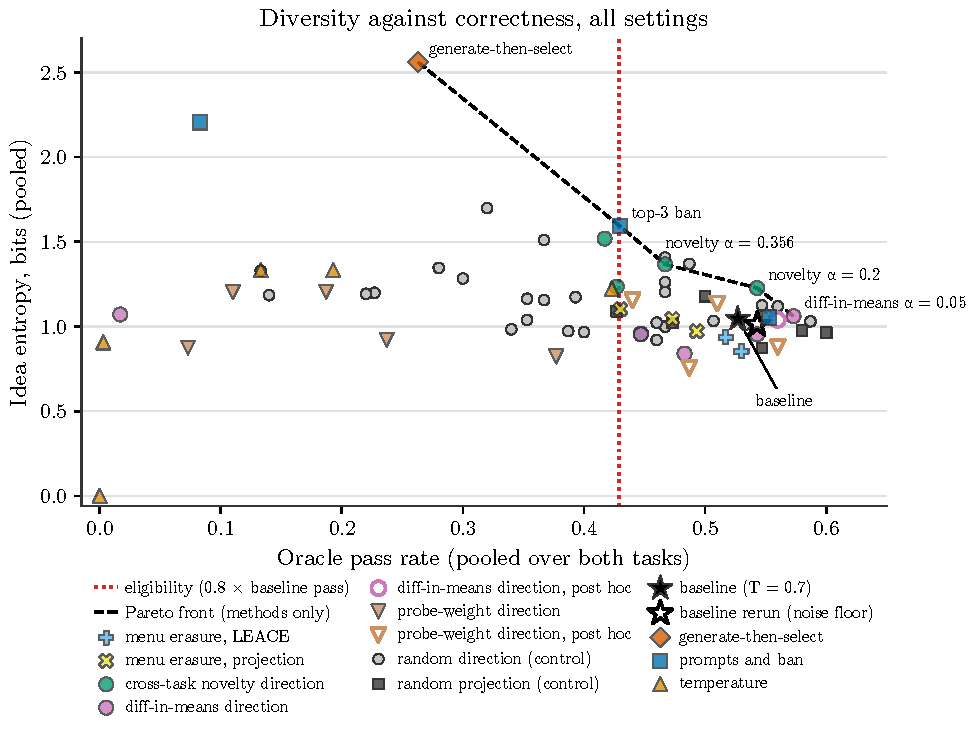
\includegraphics[width=\linewidth,height=0.85\textheight,keepaspectratio]{figures/fig_pareto_v0.pdf}
\caption{Every sweep setting plotted at its oracle pass rate (x, pooled over both tasks) and its idea entropy in bits (y, pooled). There are $n = 150$ generations per task for each method setting and 75 for each random control. Each family has its own colour and marker. Hollow markers are the post-hoc diff-in-means and probe-weight settings and the baseline rerun (the noise floor). The filled black star is the $T = 0.7$ baseline. Light-grey circles are random-direction controls and dark-grey squares are random-projection controls. The black dashed line is the Pareto front over methods. It runs through generate-then-select, the top-3 ban, novelty $\alpha = 0.356$, novelty $\alpha = 0.2$ and diff-in-means $\alpha = 0.05$. Random controls are excluded from the front, but seven of them would join it. The red dotted line marks eligibility at pass $= 0.429$ ($0.8\times$ the baseline pass rate averaged over tasks). To the right of it, the top-3 ban has the highest entropy (1.59 bits at pass 0.43). Every internal knob sits below it, among the grey random-control points. Generate-then-select reaches the highest entropy overall (2.56 bits), but at a pass rate of 0.263, which is below eligibility. Points are point estimates. A few settings coincide to within 0.005 on both axes; for example, novelty $\alpha = 2$ and diff-in-means $\alpha = 0.473$ both sit near (0.447, 0.95). [Source: artifact gen\_art\_experiment\_3, iteration 1.]}
\label{fig:fig_pareto}
\end{figure}

\begingroup\footnotesize
\setlength{\tabcolsep}{3.0pt}
\begin{longtable}{@{}>{\raggedright\arraybackslash\hspace{0pt}}p{90.55pt}>{\raggedright\arraybackslash\hspace{0pt}}p{144.68pt}>{\raggedright\arraybackslash\hspace{0pt}}p{85.62pt}>{\raggedright\arraybackslash\hspace{0pt}}p{64.01pt}>{\raggedright\arraybackslash\hspace{0pt}}p{54.88pt}@{}}
\caption{Pareto fronts (pass, metric) for each objective, with the random controls that would join them. [Source: artifact gen\_art\_experiment\_3, iteration 1.]}\label{tab:18}\\
\toprule
\textbf{objective (pooled, vs pass rate)} & \textbf{Pareto front (methods only)} & \textbf{random controls that would join the front} & \textbf{best prompt or temperature} & \textbf{best internal knob} \\
\midrule
\endfirsthead
\multicolumn{5}{@{}l}{\emph{(continued)}}\\
\toprule
\textbf{objective (pooled, vs pass rate)} & \textbf{Pareto front (methods only)} & \textbf{random controls that would join the front} & \textbf{best prompt or temperature} & \textbf{best internal knob} \\
\midrule
\endhead
\bottomrule
\endlastfoot
idea entropy & novelty direction \ensuremath{\alpha}=0.2 (0.543, 1.227); novelty direction \ensuremath{\alpha}=0.356 (0.467, 1.367); difference-in-means direction \ensuremath{\alpha}=0.05 (0.573, 1.061); generate-then-select (0.263, 2.561); top-3 ban (0.430, 1.591) & random direction \ensuremath{\alpha}=0.224, draw 2, random direction \ensuremath{\alpha}=0.473, draw 2, random direction \ensuremath{\alpha}=0.632, draw 2, random direction \ensuremath{\alpha}=1.12, draw 2, random direction \ensuremath{\alpha}=1.5, draw 2, random direction \ensuremath{\alpha}=1, draw 2, random projection a=1, draw 1 & top-3 ban (1.591) & novelty direction \ensuremath{\alpha}=0.356 (1.367) \\
off-menu correct share & novelty direction \ensuremath{\alpha}=0.356 (0.467, 0.023); difference-in-means direction \ensuremath{\alpha}=0.05 (0.573, 0.010); probe-weight direction \ensuremath{\alpha}=0.35 (post hoc) (0.560, 0.020); generate-then-select (0.263, 0.080) & random direction \ensuremath{\alpha}=0.632, draw 1, random direction \ensuremath{\alpha}=1, draw 2, random projection a=0.5, draw 2, random projection a=1, draw 1 & top-3 ban (0.023) & novelty direction \ensuremath{\alpha}=0.356 (0.023) \\
judge-confirmed novel-and-correct share & difference-in-means direction \ensuremath{\alpha}=0.05 (0.573, 0.000) & random projection a=1, draw 1 & baseline T=0.7 (0.000) & LEACE erasure a=0.5 (0.000) \\
idea entropy among passing programs & novelty direction \ensuremath{\alpha}=0.356 (0.467, 0.866); difference-in-means direction \ensuremath{\alpha}=0.05 (0.573, 0.685); probe-weight direction \ensuremath{\alpha}=0.35 (post hoc) (0.560, 0.826); generate-then-select (0.263, 1.375); top-3 ban (0.430, 1.227) & random direction \ensuremath{\alpha}=1, draw 2, random projection a=1, draw 1 & top-3 ban (1.227) & novelty direction \ensuremath{\alpha}=0.356 (0.866) \\
\end{longtable}
\endgroup
\begingroup\small
\setlength{\tabcolsep}{4.0pt}
\begin{longtable}{@{}>{\raggedright\arraybackslash\hspace{0pt}}p{45.47pt}>{\raggedright\arraybackslash\hspace{0pt}}p{297.51pt}>{\raggedright\arraybackslash\hspace{0pt}}p{102.77pt}@{}}
\caption{Ten highest-entropy eligible settings (pooled). Five of the ten are random controls. [Source: artifact gen\_art\_experiment\_3, iteration 1.]}\label{tab:19}\\
\toprule
\textbf{rank} & \textbf{setting} & \textbf{pooled idea entropy} \\
\midrule
\endfirsthead
\multicolumn{3}{@{}l}{\emph{(continued)}}\\
\toprule
\textbf{rank} & \textbf{setting} & \textbf{pooled idea entropy} \\
\midrule
\endhead
\bottomrule
\endlastfoot
1 & top-3 ban & 1.591 \\
2 & random direction \ensuremath{\alpha}=1.12, draw 2 & 1.407 \\
3 & random direction \ensuremath{\alpha}=1, draw 2 & 1.370 \\
4 & novelty direction \ensuremath{\alpha}=0.356 & 1.367 \\
5 & random direction \ensuremath{\alpha}=1.06, draw 2 & 1.262 \\
6 & novelty direction \ensuremath{\alpha}=0.2 & 1.227 \\
7 & random direction \ensuremath{\alpha}=0.632, draw 1 & 1.204 \\
8 & random projection a=0.5, draw 1 & 1.179 \\
9 & probe-weight direction \ensuremath{\alpha}=0.1 (post hoc) & 1.155 \\
10 & probe-weight direction \ensuremath{\alpha}=0.2 (post hoc) & 1.135 \\
\end{longtable}
\endgroup
\subsection{Selection, held-out draw and survival verdicts}
The selection step picked, among eligible settings on indices 0..99, the difference-in-means direction at \ensuremath{\alpha} = 0.05 (highest entropy), rank-1 projection at a = 0.25 and LEACE at a = 0.5 (on the novel-and-correct share, all tied at 0, broken by off-menu share and entropy). The probe-weight direction had no eligible setting. The best eligible temperature was T = 0.7. These were re-drawn on fresh seeds 1000..1099 with their matched controls.

\begingroup\tiny
\setlength{\tabcolsep}{1.5pt}
\begin{longtable}{@{}>{\raggedright\arraybackslash\hspace{0pt}}p{78.31pt}>{\raggedright\arraybackslash\hspace{0pt}}p{16.86pt}>{\raggedright\arraybackslash\hspace{0pt}}p{21.38pt}>{\raggedright\arraybackslash\hspace{0pt}}p{28.35pt}>{\raggedright\arraybackslash\hspace{0pt}}p{64.01pt}>{\raggedright\arraybackslash\hspace{0pt}}p{34.59pt}>{\raggedright\arraybackslash\hspace{0pt}}p{35.08pt}>{\raggedright\arraybackslash\hspace{0pt}}p{70.08pt}>{\raggedright\arraybackslash\hspace{0pt}}p{24.68pt}>{\raggedright\arraybackslash\hspace{0pt}}p{28.42pt}>{\raggedright\arraybackslash\hspace{0pt}}p{35.00pt}@{}}
\caption{Held-out draw, seeds 1000..1099 (n = 100 per task). [Source: artifact gen\_art\_experiment\_3, iteration 1.]}\label{tab:20}\\
\toprule
\textbf{setting} & \textbf{n per task} & \textbf{path: pass} & \textbf{path: idea entropy} & \textbf{path: idea labels} & \textbf{weighted: pass} & \textbf{weighted: idea entropy} & \textbf{weighted: idea labels} & \textbf{pooled pass} & \textbf{pooled idea entropy} & \textbf{eligible (path / weighted / pooled)} \\
\midrule
\endfirsthead
\multicolumn{11}{@{}l}{\emph{(continued)}}\\
\toprule
\textbf{setting} & \textbf{n per task} & \textbf{path: pass} & \textbf{path: idea entropy} & \textbf{path: idea labels} & \textbf{weighted: pass} & \textbf{weighted: idea entropy} & \textbf{weighted: idea labels} & \textbf{pooled pass} & \textbf{pooled idea entropy} & \textbf{eligible (path / weighted / pooled)} \\
\midrule
\endhead
\bottomrule
\endlastfoot
temperature 0.7, held-out & 100 & 0.700 & 1.131 & BFS 59, DFS 38, other 3 & 0.300 & 0.917 & Dijkstra 74, BFS 23, other 2, syntax error 1 & 0.500 & 1.024 & y / y / y \\
new-algorithm prompt, held-out & 100 & 0.670 & 1.667 & BFS 44, DFS 38, Dijkstra 14, bidirectional 3, A* 1 & 0.580 & 0.516 & Dijkstra 90, BFS 9, bidirectional 1 & 0.625 & 1.091 & y / y / y \\
2000-word novelty prompt, held-out & 100 & 0.100 & 2.002 & DFS 34, syntax error 27, BFS 23, other 4, random walk 3, Dijkstra 3, no code 2, greedy best-first search 1, iterative deepening 1, bidirectional 1, A* 1 & 0.060 & 2.048 & syntax error 55, Dijkstra 25, BFS 8, other 4, DFS 2, A* 1, SPFA 1, greedy best-first search 1, no code 1, bidirectional 1, Bellman-Ford 1 & 0.080 & 2.025 & n / n / n \\
top-3 ban, held-out & 100 & 0.670 & 1.378 & BFS 51, DFS 43, other 2, greedy best-first search 2, A* 1, Dijkstra 1 & 0.150 & 1.679 & Dijkstra 45, BFS 43, Bellman-Ford 4, SPFA 2, DFS 2, Floyd-Warshall 2, other 2 & 0.410 & 1.528 & y / n / n \\
difference-in-means direction \ensuremath{\alpha}=0.05, held-out & 100 & 0.750 & 1.054 & DFS 57, BFS 42, other 1 & 0.350 & 1.102 & Dijkstra 66, BFS 30, other 4 & 0.550 & 1.078 & y / y / y \\
random direction \ensuremath{\alpha}=0.05, draw 0, held-out & 100 & 0.700 & 0.965 & BFS 61, DFS 39 & 0.270 & 0.945 & Dijkstra 70, BFS 29, other 1 & 0.485 & 0.955 & y / n / y \\
rank-1 projection a=0.25, held-out & 100 & 0.700 & 0.999 & DFS 52, BFS 48 & 0.340 & 0.869 & Dijkstra 71, BFS 29 & 0.520 & 0.934 & y / y / y \\
random projection a=0.25, draw 0, held-out & 100 & 0.720 & 1.009 & BFS 64, DFS 35, other 1 & 0.290 & 0.903 & Dijkstra 73, BFS 26, other 1 & 0.505 & 0.956 & y / n / y \\
LEACE erasure a=0.5, held-out & 100 & 0.790 & 1.025 & BFS 62, DFS 37, A* 1 & 0.340 & 0.713 & Dijkstra 83, BFS 16, DFS 1 & 0.565 & 0.869 & y / y / y \\
random projection a=0.5, draw 0, held-out & 100 & 0.690 & 0.934 & BFS 65, DFS 35 & 0.320 & 1.005 & Dijkstra 73, BFS 24, other 2, SPFA 1 & 0.505 & 0.969 & y / y / y \\
\end{longtable}
\endgroup
On the held-out draw the difference-in-means direction gives 0.93x the entropy of the held-out T = 0.7 draw on the open task and 1.20x on the weighted task, against a required 2x, and its CI against the random direction includes 0 on both tasks. Nothing survives (\texttt{gen\_\allowbreak{}art\_\allowbreak{}experiment\_\allowbreak{}3}).

\begingroup\footnotesize
\setlength{\tabcolsep}{3.0pt}
\begin{longtable}{@{}>{\raggedright\arraybackslash\hspace{0pt}}p{94.54pt}>{\raggedright\arraybackslash\hspace{0pt}}p{94.69pt}>{\raggedright\arraybackslash\hspace{0pt}}p{130.15pt}>{\raggedright\arraybackslash\hspace{0pt}}p{83.25pt}>{\raggedright\arraybackslash\hspace{0pt}}p{37.12pt}@{}}
\caption{Pre-registered survival verdicts. [Source: artifact gen\_art\_experiment\_3, iteration 1.]}\label{tab:21}\\
\toprule
\textbf{knob family} & \textbf{selected setting (indices 0..99)} & \textbf{rule} & \textbf{held-out numbers} & \textbf{verdict} \\
\midrule
\endfirsthead
\multicolumn{5}{@{}l}{\emph{(continued)}}\\
\toprule
\textbf{knob family} & \textbf{selected setting (indices 0..99)} & \textbf{rule} & \textbf{held-out numbers} & \textbf{verdict} \\
\midrule
\endhead
\bottomrule
\endlastfoot
probe-weight flattening & none & entropy \ensuremath{\geq} 2\ensuremath{\times} best eligible temperature and CI vs random direction excludes 0 & no eligible setting at matched pass rate & fails \\
difference-in-means flattening & difference-in-means direction \ensuremath{\alpha}=0.05 & same & path: entropy 1.054 vs 1.131 (ratio 0.932), diff vs random 0.090 [-0.054, 0.234], pass 0.75; weighted: 1.102 vs 0.917 (ratio 1.203), diff 0.158 [-0.069, 0.367], pass 0.35; pooled 1.078 vs 1.024, diff 0.124 [-0.019, 0.251] & fails \\
menu erasure, rank-1 projection & rank-1 projection a=0.25 & judge-confirmed novel-and-correct share \ensuremath{\geq} 3\ensuremath{\times} best of temperature/prompts/ban, \ensuremath{\geq} 0.05 absolute, CI vs random projection excludes 0 & share 0.000 (comparators all 0.000); rule-only upper bound 0.000; pass 0.520 & fails \\
menu erasure, LEACE & LEACE erasure a=0.5 & judge-confirmed novel-and-correct share \ensuremath{\geq} 3\ensuremath{\times} best of temperature/prompts/ban, \ensuremath{\geq} 0.05 absolute, CI vs random projection excludes 0 & share 0.000 (comparators all 0.000); rule-only upper bound 0.000; pass 0.565 & fails \\
cross-task novelty direction & all 5 strengths (no selection) & Spearman(\ensuremath{\alpha}, atypicality) \ensuremath{\geq} 0.8 on both tasks and top strength beats random & Spearman path 0.486 [-0.029, 0.543], weighted -0.257 [-0.486, 0.143]; top vs random path -0.176 [-0.529, 0.187], weighted -0.313 [-0.612, -0.041] & fails \\
\end{longtable}
\endgroup
\begingroup\footnotesize
\setlength{\tabcolsep}{3.0pt}
\begin{longtable}{@{}>{\raggedright\arraybackslash\hspace{0pt}}p{126.89pt}>{\raggedright\arraybackslash\hspace{0pt}}p{75.36pt}>{\raggedright\arraybackslash\hspace{0pt}}p{74.69pt}>{\raggedright\arraybackslash\hspace{0pt}}p{82.02pt}>{\raggedright\arraybackslash\hspace{0pt}}p{80.79pt}@{}}
\caption{Targeted additive settings against the pooled random directions at the same strength (unpaired bootstrap; * = CI excludes 0). [Source: artifact gen\_art\_experiment\_3, iteration 1.]}\label{tab:22}\\
\toprule
\textbf{setting} & \textbf{path: \ensuremath{\Delta} entropy vs random [95\% CI]} & \textbf{path: \ensuremath{\Delta} pass vs random [95\% CI]} & \textbf{weighted: \ensuremath{\Delta} entropy [95\% CI]} & \textbf{weighted: \ensuremath{\Delta} pass [95\% CI]} \\
\midrule
\endfirsthead
\multicolumn{5}{@{}l}{\emph{(continued)}}\\
\toprule
\textbf{setting} & \textbf{path: \ensuremath{\Delta} entropy vs random [95\% CI]} & \textbf{path: \ensuremath{\Delta} pass vs random [95\% CI]} & \textbf{weighted: \ensuremath{\Delta} entropy [95\% CI]} & \textbf{weighted: \ensuremath{\Delta} pass [95\% CI]} \\
\midrule
\endhead
\bottomrule
\endlastfoot
novelty direction \ensuremath{\alpha}=0.632 & +0.496 [+0.252, +0.719] * & -0.169 [-0.267, -0.064] * & +0.118 [-0.154, +0.383] & -0.007 [-0.104, +0.096] \\
novelty direction \ensuremath{\alpha}=1.12 & +0.092 [-0.166, +0.319] & -0.018 [-0.120, +0.096] & -0.454 [-0.748, -0.156] * & +0.067 [-0.033, +0.160] \\
novelty direction \ensuremath{\alpha}=2 & -0.219 [-0.514, +0.101] & +0.367 [+0.278, +0.462] * & -0.456 [-0.788, -0.075] * & +0.198 [+0.113, +0.282] * \\
difference-in-means direction \ensuremath{\alpha}=0.224 & -0.892 [-1.092, -0.678] * & -0.013 [-0.113, +0.078] & +0.374 [+0.130, +0.584] * & -0.087 [-0.182, +0.007] \\
difference-in-means direction \ensuremath{\alpha}=0.473 & -0.713 [-0.946, -0.475] * & -0.069 [-0.171, +0.029] & +0.302 [+0.058, +0.533] * & +0.024 [-0.071, +0.124] \\
difference-in-means direction \ensuremath{\alpha}=1 & -0.287 [-1.391, -0.196] * & -0.591 [-0.653, -0.524] * & -0.210 [-0.762, +0.149] & -0.202 [-0.262, -0.142] * \\
probe-weight direction \ensuremath{\alpha}=1.06 & -0.498 [-0.805, -0.173] * & -0.282 [-0.380, -0.187] * & +0.278 [+0.028, +0.497] * & -0.158 [-0.233, -0.076] * \\
probe-weight direction \ensuremath{\alpha}=1.26 & -0.463 [-0.637, -0.313] * & -0.389 [-0.453, -0.324] * & -0.201 [-0.546, +0.102] & -0.022 [-0.107, +0.058] \\
probe-weight direction \ensuremath{\alpha}=1.5 & -0.634 [-0.923, -0.434] * & -0.429 [-0.493, -0.367] * & -0.763 [-1.124, -0.427] * & -0.064 [-0.140, +0.004] \\
\end{longtable}
\endgroup
The cross-task novelty direction fails its own test in an instructive way. Atypicality rises from \ensuremath{\alpha} = 0 to 0.632 on the open task (0.835 to 1.675) and then falls back (1.064 at \ensuremath{\alpha} = 2.0); on the weighted task it never rises consistently. The rule required Spearman at least 0.8 on both tasks; the values are 0.486 and \ensuremath{-}0.257. At the top strength the direction is less atypical than random directions on the weighted task (CI excludes 0 in the wrong direction).

\begin{figure}[!htbp]
\centering
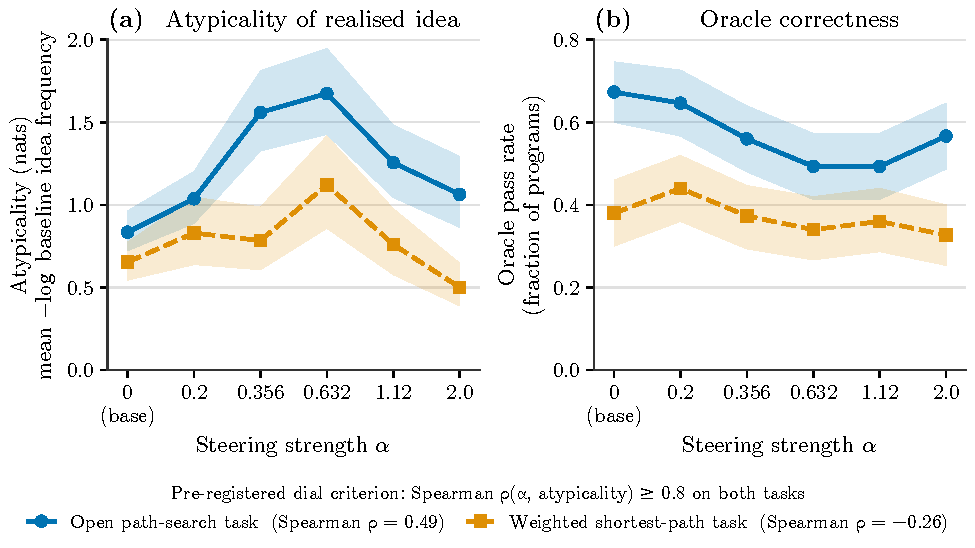
\includegraphics[width=\linewidth,height=0.85\textheight,keepaspectratio]{figures/fig_a4_v0.pdf}
\caption{Dose-response of the cross-task novelty direction (extracted from five non-path tasks and added at layers 29--31 of Qwen2.5-3B-Instruct). The $x$-axis is the steering strength $\alpha$, drawn as categories ($\alpha = 0$ is the unsteered baseline). Blue circles with solid lines show the open path-search task; orange squares with dashed lines show the weighted shortest-path task. Each point is the mean over $n = 150$ programs, and the shaded bands are 95\% percentile-bootstrap intervals over those programs. (a)~Atypicality of the realised idea: the mean $-\log$ baseline frequency of the algorithm the program implements, in nats. (b)~Oracle pass rate, the fraction of programs that pass all 50 test graphs. Atypicality is not monotone in $\alpha$. On the open task it rises from 0.83 to a peak of 1.67 at $\alpha = 0.632$ and falls back to 1.06 at $\alpha = 2$; on the weighted task it never rises consistently and ends below baseline (0.50 vs.\ 0.65). The legend gives Spearman $\rho(\alpha, \text{atypicality})$: 0.49 (open) and $-0.26$ (weighted), against the pre-registered criterion of $\rho \ge 0.8$ on both tasks (exact permutation $p = 0.36$ and $0.66$). Pass rate falls from 0.67 to 0.49 on the open task under steering. So the direction fails as a dial, even though it detects novelty requests on held-out path tasks with AUROC 1.0. [Source: artifact gen\_art\_experiment\_3, iteration 1; exact permutation p from gen\_art\_experiment\_6, iteration 2.]}
\label{fig:fig_a4}
\end{figure}

\begingroup\footnotesize
\setlength{\tabcolsep}{3.0pt}
\begin{longtable}{@{}>{\raggedright\arraybackslash\hspace{0pt}}p{100.00pt}>{\raggedright\arraybackslash\hspace{0pt}}p{97.70pt}>{\raggedright\arraybackslash\hspace{0pt}}p{59.44pt}>{\raggedright\arraybackslash\hspace{0pt}}p{100.68pt}>{\raggedright\arraybackslash\hspace{0pt}}p{81.94pt}@{}}
\caption{Cross-task novelty direction: dose-response used by the survival rule (\ensuremath{\alpha} = 0 is the baseline). [Source: artifact gen\_art\_experiment\_3, iteration 1.]}\label{tab:23}\\
\toprule
\textbf{strength \ensuremath{\alpha}} & \textbf{path: atypicality} & \textbf{path: pass} & \textbf{weighted: atypicality} & \textbf{weighted: pass} \\
\midrule
\endfirsthead
\multicolumn{5}{@{}l}{\emph{(continued)}}\\
\toprule
\textbf{strength \ensuremath{\alpha}} & \textbf{path: atypicality} & \textbf{path: pass} & \textbf{weighted: atypicality} & \textbf{weighted: pass} \\
\midrule
\endhead
\bottomrule
\endlastfoot
0.0 & 0.835 & 0.673 & 0.654 & 0.380 \\
0.2 & 1.037 & 0.647 & 0.830 & 0.440 \\
0.356 & 1.560 & 0.560 & 0.784 & 0.373 \\
0.632 & 1.675 & 0.493 & 1.121 & 0.340 \\
1.12 & 1.256 & 0.493 & 0.760 & 0.360 \\
2.0 & 1.064 & 0.567 & 0.501 & 0.327 \\
slope of \ensuremath{\Delta}log p vs \ensuremath{-}log p0 at top strength & 0.242 &  & 0.230 &  \\
\end{longtable}
\endgroup
\begin{correction}\textbf{Correction (iteration 2).} The Spearman confidence intervals in Table 21 came from resampling samples within each strength cell with the baseline frequencies p0 held fixed, which is why the open-task point estimate 0.486 sat at the edge of its interval [\ensuremath{-}0.029, 0.543]. With six strength points Spearman's rho takes only multiples of 1/35. The exact permutation p-values (720 permutations) are 0.36 on the open task and 0.66 on the weighted task, two-sided; a bootstrap that also resamples the baseline gives [\ensuremath{-}0.43, 0.60] and [\ensuremath{-}1.00, 0.09] (\texttt{gen\_\allowbreak{}art\_\allowbreak{}experiment\_\allowbreak{}6}). The verdict is unchanged.\end{correction}
\subsection{Manipulation checks: the steering does what it was built to do internally, and the output follows only partly}
Baseline probes (trained on unsteered mean(gen1..32) residuals) were applied to the residuals captured during steered generation, at layer 30 (band middle) and layer 33 (downstream). Two quantities are reported: the probe menu entropy, defined as the entropy of the probe softmax restricted to the menu, and the probe decodability, defined as the balanced accuracy with which the probe predicts the realised idea of each steered sample. For the flattening directions the probe menu entropy goes to 0.000 bits at every strength from \ensuremath{\alpha} = 0.224 (difference-in-means; from \ensuremath{\alpha} = 0.106 on the open task) and at every probe-weight strength: the steered state reads as one idea with full confidence, the opposite of flattening, and consistent with the DFS takeover in the outputs. For erasure, probe decodability drops to 0.27 to 0.44 at full strength (unsteered rerun: 0.48 and 0.57), yet the outputs remain BFS, DFS and Dijkstra. The internal readout can be erased without the behaviour changing.

\begingroup\scriptsize
\setlength{\tabcolsep}{2.0pt}
\begin{longtable}{@{}>{\raggedright\arraybackslash\hspace{0pt}}p{77.98pt}>{\raggedright\arraybackslash\hspace{0pt}}p{31.52pt}>{\raggedright\arraybackslash\hspace{0pt}}p{53.11pt}>{\raggedright\arraybackslash\hspace{0pt}}p{31.50pt}>{\raggedright\arraybackslash\hspace{0pt}}p{53.10pt}>{\raggedright\arraybackslash\hspace{0pt}}p{40.15pt}>{\raggedright\arraybackslash\hspace{0pt}}p{53.11pt}>{\raggedright\arraybackslash\hspace{0pt}}p{40.15pt}>{\raggedright\arraybackslash\hspace{0pt}}p{53.11pt}@{}}
\caption{Manipulation checks with baseline probes on steered residuals (unsteered reference rows first). [Source: artifact gen\_art\_experiment\_3, iteration 1.]}\label{tab:24}\\
\toprule
\textbf{setting} & \textbf{path, layer 30: probe menu entropy (bits)} & \textbf{path, layer 30: probe decodability} & \textbf{path, layer 33: menu entropy} & \textbf{path, layer 33: decodability} & \textbf{weighted, layer 30: menu entropy} & \textbf{weighted, layer 30: decodability} & \textbf{weighted, layer 33: menu entropy} & \textbf{weighted, layer 33: decodability} \\
\midrule
\endfirsthead
\multicolumn{9}{@{}l}{\emph{(continued)}}\\
\toprule
\textbf{setting} & \textbf{path, layer 30: probe menu entropy (bits)} & \textbf{path, layer 30: probe decodability} & \textbf{path, layer 33: menu entropy} & \textbf{path, layer 33: decodability} & \textbf{weighted, layer 30: menu entropy} & \textbf{weighted, layer 30: decodability} & \textbf{weighted, layer 33: menu entropy} & \textbf{weighted, layer 33: decodability} \\
\midrule
\endhead
\bottomrule
\endlastfoot
baseline rerun (noise floor) & 0.181 & 0.481 & 0.274 & 0.489 & 0.128 & 0.574 & 0.186 & 0.577 \\
temperature 0.7, held-out & 0.233 & 0.484 & 0.322 & 0.475 & 0.152 & 0.594 & 0.201 & 0.565 \\
temperature 1.0 & 0.165 & 0.570 & 0.237 & 0.655 & 0.168 & 0.417 & 0.222 & 0.424 \\
top-3 ban & 0.273 & 0.403 & 0.410 & 0.410 & 0.300 & 0.361 & 0.330 & 0.329 \\
new-algorithm prompt & 0.138 & 0.463 & 0.190 & 0.583 & 0.059 & 0.414 & 0.069 & 0.456 \\
2000-word novelty prompt & 0.173 & 0.327 & 0.350 & 0.323 & 0.334 & 0.323 & 0.340 & 0.287 \\
probe-weight direction \ensuremath{\alpha}=0.75 & 0.000 & 0.500 & 0.000 & 0.500 & 0.000 & 0.250 & 0.000 & 0.250 \\
probe-weight direction \ensuremath{\alpha}=0.892 & 0.000 & 0.333 & 0.000 & 0.333 & 0.000 & 0.250 & 0.000 & 0.250 \\
probe-weight direction \ensuremath{\alpha}=1.06 & 0.000 & 0.250 & 0.000 & 0.250 & 0.000 & 0.250 & 0.000 & 0.250 \\
probe-weight direction \ensuremath{\alpha}=1.26 & 0.000 & 0.500 & 0.000 & 0.500 & 0.000 & 0.250 & 0.000 & 0.250 \\
probe-weight direction \ensuremath{\alpha}=1.5 & 0.000 & 0.500 & 0.000 & 0.500 & 0.000 & 0.250 & 0.000 & 0.250 \\
difference-in-means direction \ensuremath{\alpha}=0.05 & 0.109 & 0.526 & 0.153 & 0.564 & 0.162 & 0.553 & 0.226 & 0.553 \\
difference-in-means direction \ensuremath{\alpha}=0.106 & 0.000 & 0.333 & 0.009 & 0.333 & 0.209 & 0.401 & 0.183 & 0.394 \\
difference-in-means direction \ensuremath{\alpha}=0.224 & 0.000 & 0.333 & 0.000 & 0.333 & 0.000 & 0.250 & 0.000 & 0.250 \\
difference-in-means direction \ensuremath{\alpha}=0.473 & 0.000 & 0.333 & 0.000 & 0.333 & 0.000 & 0.250 & 0.000 & 0.250 \\
difference-in-means direction \ensuremath{\alpha}=1 & 0.000 & 0.500 & 0.000 & 0.500 & 0.000 & 0.333 & 0.000 & 0.333 \\
rank-1 projection a=0.25 & 0.169 & 0.645 & 0.292 & 0.668 & 0.127 & 0.509 & 0.177 & 0.522 \\
rank-1 projection a=0.5 & 0.108 & 0.462 & 0.224 & 0.516 & 0.147 & 0.360 & 0.221 & 0.398 \\
rank-1 projection a=0.75 & 0.162 & 0.431 & 0.242 & 0.476 & 0.116 & 0.336 & 0.169 & 0.384 \\
rank-1 projection a=1 & 0.175 & 0.436 & 0.227 & 0.466 & 0.093 & 0.273 & 0.144 & 0.281 \\
LEACE erasure a=0.5 & 0.290 & 0.282 & 0.408 & 0.427 & 0.117 & 0.294 & 0.116 & 0.288 \\
LEACE erasure a=1 & 0.085 & 0.392 & 0.192 & 0.526 & 0.114 & 0.286 & 0.081 & 0.292 \\
novelty direction \ensuremath{\alpha}=0.2 & 0.150 & 0.600 & 0.294 & 0.571 & 0.099 & 0.382 & 0.381 & 0.377 \\
novelty direction \ensuremath{\alpha}=0.356 & 0.146 & 0.394 & 0.290 & 0.544 & 0.034 & 0.337 & 0.311 & 0.422 \\
novelty direction \ensuremath{\alpha}=0.632 & 0.015 & 0.250 & 0.355 & 0.371 & 0.064 & 0.319 & 0.431 & 0.277 \\
novelty direction \ensuremath{\alpha}=1.12 & 0.003 & 0.250 & 0.172 & 0.245 & 0.202 & 0.250 & 0.001 & 0.250 \\
novelty direction \ensuremath{\alpha}=2 & 0.000 & 0.250 & 0.000 & 0.250 & 0.129 & 0.250 & 0.000 & 0.250 \\
\end{longtable}
\endgroup
\subsection{Novelty: the judge found no novel correct program in any condition}
Every distinct passing program in the catch-all class of the classifier, across the sweep and the held-out draw, was sent to the judge: 70 programs (\texttt{gen\_\allowbreak{}art\_\allowbreak{}experiment\_\allowbreak{}3}). All 70 were judged to be known algorithms, most often Dijkstra written in an unusual way (41). The judge-confirmed novel-and-correct share is therefore 0 in every condition, including generate-then-select and the 2000-word novelty prompt. Over all 267 judge calls (audit plus novelty checks) the verdicts were: Dijkstra 81, BFS 45, other (known) 31, DFS 25, Bellman-Ford 23, A* 18, Floyd-Warshall 17, iterative deepening 8, bidirectional 7, random walk 7, unparsed 4, greedy best-first search 1. Judge spend was \$0.081 against a \$1.5 cap.

\begingroup\small
\setlength{\tabcolsep}{4.0pt}
\begin{longtable}{@{}>{\raggedright\arraybackslash\hspace{0pt}}p{198.01pt}>{\raggedright\arraybackslash\hspace{0pt}}p{79.93pt}>{\raggedright\arraybackslash\hspace{0pt}}p{100.67pt}>{\raggedright\arraybackslash\hspace{0pt}}p{59.14pt}@{}}
\caption{Judge verdicts on the 70 distinct passing programs in the catch-all class of the classifier. [Source: artifact gen\_art\_experiment\_3, iteration 1.]}\label{tab:25}\\
\toprule
\textbf{judge verdict} & \textbf{open path search} & \textbf{weighted shortest path} & \textbf{total} \\
\midrule
\endfirsthead
\multicolumn{4}{@{}l}{\emph{(continued)}}\\
\toprule
\textbf{judge verdict} & \textbf{open path search} & \textbf{weighted shortest path} & \textbf{total} \\
\midrule
\endhead
\bottomrule
\endlastfoot
Dijkstra & 4 & 37 & 41 \\
other (known) & 11 & 1 & 12 \\
Bellman-Ford & 0 & 7 & 7 \\
BFS & 7 & 0 & 7 \\
DFS & 3 & 0 & 3 \\
distinct novel algorithm & 0 & 0 & 0 \\
\textbf{all} & 25 & 45 & 70 \\
\end{longtable}
\endgroup
\subsection{Noise floor and independent verification}
Regenerating the baseline in differently composed batches flips 16.7\% of open-task and 10.7\% of weighted-task idea labels at the same seeds (the noise-floor rerun row in Table 10), because bf16 numerics depend on batch composition. Common random numbers therefore pair conditions only approximately, and the per-sample flip rates in Tables 16 and 17 have a floor of roughly 0.11 to 0.17. An independent re-derivation script, with its own oracle runner, a coarse independent classifier and a separate recomputation of every metric, reproduces the stored numbers. The placebo test also shows that the bootstrap CIs are somewhat anticonservative: random splits of the baseline produce a CI excluding 0 at a rate of 0.10 and 0.15 instead of 0.05, which matters for any claim resting on a CI that barely excludes 0. None of the iteration's verdicts rests on such a claim, because nothing came close to the survival margins.

\begingroup\small
\setlength{\tabcolsep}{4.0pt}
\begin{longtable}{@{}>{\raggedright\arraybackslash\hspace{0pt}}p{280.74pt}>{\raggedright\arraybackslash\hspace{0pt}}p{173.01pt}@{}}
\caption{Independent verification and placebo checks. [Source: artifact gen\_art\_experiment\_3, iteration 1.]}\label{tab:26}\\
\toprule
\textbf{check} & \textbf{result} \\
\midrule
\endfirsthead
\multicolumn{2}{@{}l}{\emph{(continued)}}\\
\toprule
\textbf{check} & \textbf{result} \\
\midrule
\endhead
\bottomrule
\endlastfoot
independent oracle runner vs stored pass/fail & 1.000 agreement on 147 programs \\
coarse independent classifier vs AST classifier & 0.973 agreement \\
entropy difference, open path search, baseline vs noise-floor rerun (placebo) & 95\% CI [-0.182, 0.281], excludes 0: False \\
entropy difference, weighted shortest path, baseline vs noise-floor rerun (placebo) & 95\% CI [-0.189, 0.228], excludes 0: False \\
entropy difference, open path search, top-3 ban vs baseline (real effect) & 95\% CI [-0.035, 0.445], excludes 0: False \\
entropy difference, weighted shortest path, top-3 ban vs baseline (real effect) & 95\% CI [0.560, 1.103], excludes 0: True \\
rate at which a random split of the baseline yields a CI excluding 0 & path 0.10, weighted 0.15 (nominal 0.05) \\
\end{longtable}
\endgroup
\subsection{Bookkeeping}
\begin{itemize}
\item Artifact: gen\_art\_experiment\_3. 19,250 generations in total, in 111 setting files per task (baseline, calibration, sweep, held-out, post-hoc, generate-then-select). Pipeline stages and wall-clock times as recorded: baseline about 5 min, activation cache 2 min, probes 2 min, vectors 3 min, calibration 4 min, sweep about 65 min, post-sweep chain (judge, select, held-out, judge, analyse) about 25 min, post-hoc settings 5 min, verification 4 min; roughly two GPU-hours on one RTX PRO 4500 (32 GB).
\end{itemize}
\begin{correction}\textbf{Correction (iteration 2).} The file counts are not 111 per task. The open task has 111 generation files and 110 scored files; the weighted task has 81 and 80. The difference is the 30 calibration files (\texttt{calib\_\allowbreak{}A4\_\allowbreak{}*}, \texttt{calib\_\allowbreak{}Hdim\_\allowbreak{}*}, \texttt{calib\_\allowbreak{}Hprobe\_\allowbreak{}*}, ten strengths each), which exist only for the open task, and the generate-then-select stage-1 list file \texttt{gts\_\allowbreak{}list}, which has no scored counterpart (\texttt{gen\_\allowbreak{}art\_\allowbreak{}experiment\_\allowbreak{}6}). The 19,250 total is correct.\end{correction}
\begin{itemize}
\item The first sweep launch was stopped after about 2,400 generations because of CUDA allocator thrashing and resumed from the per-setting files with \texttt{PYTORCH\_\allowbreak{}CUDA\_\allowbreak{}ALLOC\_\allowbreak{}CONF=\allowbreak{}expandable\_\allowbreak{}segments:\allowbreak{}True} (allocator only, no change to numerics). Two held-out files whose scoring thread crashed on a malformed return were scored afterwards by \texttt{score\_\allowbreak{}backlog.py}.
\item Deviations from the plan, all recorded in the artifact: the late-window probe feature and hook window; menus exclude the catch-all class, so k = 2 and erasure is rank 1; oracle runs only the requested code; code-block early stop for all conditions; n = 150 and 75 instead of the planned 100 and 50, with a 100-seed held-out draw; post-hoc low-strength flattening settings reported but excluded from survival; a single model.
\item Kept on the run volume only (not in the published repository): \texttt{acts/} (0.9 GB baseline residuals, split into parts under 100 MB) and \texttt{caps/} (0.9 GB residuals captured during steering). Published: generations, scored rows, judge verdicts, vectors (\texttt{vectors/vectors.pt} and one LEACE eraser file per task, \texttt{vectors/leace\_\allowbreak{}*.pt}), figures and results files.
\item The external judge model was the only paid call: \$0.081.
\item Files: pre-registered rules \texttt{results/rules.json} (frozen 2026-10-15 ); all metrics and CIs \texttt{results/results.json}; independent re-derivation \texttt{verify\_\allowbreak{}headline.py} \ensuremath{\rightarrow} \texttt{results/verify\_\allowbreak{}headline.json}; PCA view \texttt{figs/fig\_\allowbreak{}pca\_\allowbreak{}manifold.png}; artifact figures \texttt{figs/} (probe curve, three Pareto fronts, fraction-correct violins, novelty-direction dose-response, idea shares, PCA view); schema output \texttt{method\_\allowbreak{}out.json} with \texttt{full\_\allowbreak{}}, \texttt{mini\_\allowbreak{}} and \texttt{preview\_\allowbreak{}} variants.
\end{itemize}
\subsection{What iteration 1 established, and what it did not}
\textbf{Established, on one model and two tasks.}

\begin{enumerate}
\item The internal knobs tested here are selectors, not diversifiers. A single residual direction at layers 29 to 31, built from baseline activations, moves the open task from two-thirds BFS to 97\% DFS without costing correctness. This is controllable choice among ideas the model already writes. No knob produced an idea outside the model's usual repertoire.
\item Under the pre-registered rules no internal knob beats the practitioner knobs: the difference-in-means direction reached 0.93x and 1.20x the entropy of the best eligible temperature on held-out seeds (2x required), menu erasure produced no novel correct program, and the cross-task novelty direction was not monotone in strength. The headline the rules prescribe is the prompting ceiling, with the top-3 ban atop the eligible entropy front and generate-then-select atop the full front.
\item Matched-norm random directions raise idea entropy about as much as targeted ones, and five of the ten highest-entropy eligible settings are random controls. Most of the diversity that steering buys here is non-specific perturbation.
\item Temperature is not a creativity knob for this model on these tasks. Its eligible range ends at T = 0.7; above that, correctness collapses while idea entropy gains a few tenths of a bit and no new idea class appears above 5\% of samples.
\item Bans are mostly ignored by this 3B model (87\% to 95\% of programs still use a banned idea), and on the weighted task the ban moves mass from the correct menu idea to the incorrect one.
\item Novelty, defined strictly as a correct program the judge does not recognise as a known algorithm, was zero in every condition.
\item The idea is not linearly decodable from the prompt-final token or the first 8 generated tokens; it becomes decodable from the mean over the first 32 generated tokens, which cover the explanatory preamble, at about the same level at every layer.
\end{enumerate}
\begin{correction}\textbf{Correction (iteration 2).} Three of these conclusions are revised by later evidence. Conclusion 3 (random parity) does not hold as stated once targeted settings are compared with the draw-averaged random entropy (Section 2.9). Conclusion 5 generalised from one prompt protocol to the model: non-compliance is 87\% to 95\% under the contract prompt with list-style wording, and 0\% to 46\% under the bare prompt with short-list wording (61\% for the weighted-task top-5 list) (Section 2.4). Conclusion 6 is near-floor by construction on textbook tasks and only covered passing programs that the classifier put in its catch-all class; it is restated in the closing section as "no condition produced a correct program that a judge did not recognise". All seven conclusions are conditional on the contract prompt.\end{correction}
\textbf{Dead ends recorded as such.}

\begin{itemize}
\item \emph{Flattening the idea utilities as a novelty knob (the main hypothesis's claim about direct utility edits).} Killed by Table 12, the idea-composition figure in Section 1.10 and Table 24: the flattening directions select the minority idea, the internal readout collapses to one idea, and the held-out entropy ratio is 0.93 and 1.20 against a required 2.
\item \emph{Menu erasure as a route to novelty (the menu-erasure alternative).} Killed by Tables 13 and 25: erasure removes idea decodability offline (weighted task 0.888 to 0.334) and online (0.27 to 0.44), but the outputs remain BFS, DFS and Dijkstra and the novel-and-correct share is 0.
\item \emph{A single portable unusualness dial (the unusualness-dial alternative).} Killed as a dial by Table 23 (Spearman 0.486 and \ensuremath{-}0.257, required 0.8), although the direction transfers perfectly as a readout (AUROC 1.0, Table 8). Reading whether novelty was requested is easy; turning that reading into atypical outputs did not work.
\item \emph{Probing the first 8 tokens for the choice.} The planned probe feature carried only task identity (Table 4).
\item \emph{Temperature arm and ban arm.} Not delivered; no evidence either way from them.
\end{itemize}
\textbf{Open after iteration 1.}

\begin{itemize}
\item Whether the temperature law holds (straight Arrhenius lines, no reordering) or the gradual-commitment alternative holds; the influence arm's temperature rows show no reordering among the two menu ideas but cover only T = 0.7 to 1.3 with usable output.
\item Where the commitment point is per sample (forking-path resampling), and whether a utility vector read there predicts temperature, seed and ban effects.
\item Seeds: untested.
\item Where banned probability goes (nearest neighbour, far side, or proportional): the influence arm's single ban shows mostly non-compliance, which by itself argues that a 3B model may be the wrong place to test substitution structure, since there is little banned mass to redistribute.
\end{itemize}
\begin{correction}\textbf{Correction (iteration 2).} The ban arm's bare-prompt data, unreported at the time, show large compliance and structured substitution in this same 3B model (Section 2.4), so the argument that a 3B model has too little banned mass to redistribute is withdrawn.\end{correction}
\begin{itemize}
\item Whether the selector finding generalises to the reserved model and task.
\end{itemize}
\subsection{Review and hypothesis update for iteration 1 (from the round record)}\label{sec:rec1}

This subsection is typeset from the run's structured round record, not from the report draft. It gives the reviewer's verdict on iteration 1 and the hypothesis update that followed it, in the record's own words (identifiers removed).

\paragraph{Strategy and plans.}

The iteration ran one strategy, \emph{Screening rival theories of LLM idea choice}. Its objective, as recorded: Run a pre-registered three-arm screen on one open-weight instruction model (Qwen2.5-3B-Instruct) and identical tasks, prompts and idea classifier. It decides which mechanistic account of 'LLM creativity' survives on each of the three knob families the user asked about. TEMPERATURE: a single early commitment fork with a readable utility vector, where heat flattens but never reorders (H), vs gradual multi-path commitment, where heat reorders toward 'entropic' ideas (A1). BANS: nested-logit substitution to the banned idea's nearest internal neighbour (H) vs repulsion to the far side of the idea manifold (A2) vs plain IIA renormalisation (null). INTERNAL INFLUENCE: flattening the utility vector at the commitment layer (H) vs erasing the menu subspace (A3) vs a task-general 'unusualness' direction (A4), all against tuned temperature, novelty prompts, bans and random-direction controls at matched correctness. The output is a ranked comparison with effect sizes, one survivor per knob family, and reusable building blocks (classified generations, activations, classifier and oracle code). Iteration 2 then confirms the survivors on the reserved model and task.

Rationale, as recorded: The hypothesis bundles three separable claims, and each has a rival alternate that predicts the OPPOSITE observable on the same data. That makes a cheap wide screen decisive in a way a deep test of H alone could not be. (1) H predicts straight Arrhenius lines, no top-3 reversals for T\textless{}=1.3, and a sharp single fork; A1 predicts curvature, reversals at high T, and many partial forks whose count predicts which ideas gain with heat. One temperature grid plus forking-path resampling settles it. (2) H predicts that post-ban mass lands closer in activation space to the banned centroids than the baseline average; A2 predicts it lands farther; IIA predicts no geometric structure. One ban set with geometry from unbanned runs settles it. (3) H, A3 and A4 are three different internal edits that can be put on one Pareto plot of idea entropy and outside-menu correct share vs pass rate, against the knobs practitioners actually use. Each arm answers a concrete question from the user's request. Arm 1 covers the a/b/c questions (ideas vs phrasings under temperature and top-k=10), via an alpha/beta Hill-number partition, and the 'mean vs mode' question, via a utility-vector readout. Arm 2 covers the 'ban the top 5: edge or opposite side of the manifold?' question, with the manifold plot. Arm 3 covers 'can we make LLMs give truly novel solutions?', with the seed-shock comparison as a cheap add-on. All arms aim at positive, lead-able results. Arm 1 targets a quantitative temperature law, Arm 2 a measured IIA violation with a geometric predictor (no prior work studies substitution structure among ideas), and Arm 3 an internal knob that dominates temperature at matched correctness. A null in any arm is still a clean mechanistic finding, because the rival in that arm wins. This is the first iteration and no dataset exists, so each experiment generates its own data under the shared protocol and saves it for iteration 2.

Plans executed under it:

\begin{itemize}

\item Does temperature change ideas or just wording? (experiment)

\item Where do banned ideas go? (ban arm) (experiment)

\item Can internal knobs beat temperature for novel code? (experiment)

\end{itemize}

\paragraph{Reviewer verdict.}

Overall score 4; blocking: yes; coverage judged partial; dimension scores: soundness 1, presentation 3, contribution 2. The reviewer's overall assessment:

\begin{quote}\small

The influence arm (the artifact) is recorded thoroughly and its numbers hold. I recomputed the main ones from scored/\{T1,T3\}/*.jsonl (recompute.py -\textgreater{} recompute\_out.json) and every one matched: baseline T1 BFS 205/DFS 80, pass 0.700; T3 Dijkstra 225/BFS 71, pass 0.373; sweep baseline H = 1.175/0.916 bits; top-3 ban H = 1.404/1.779 with 142/150 and 131/150 programs still using a banned idea; generate-then-select H = 2.549/2.574; H-dim a=0.224 gives DFS 145/150 at pass 0.680; held-out entropy ratios 0.932/1.202; 19,250 generations. Survival verdicts, the classifier audit and judge cost match results/results.json. results\_reported is therefore true.

The record is still badly incomplete, and that omission changes conclusions. Section 1.2 says the ban arm 'failed with a model-API streaming error before producing results'. On disk, gen\_art\_experiment\_2 holds 4,360 completed generations, 4,210 of them labelled: 3 tasks x \{baseline n=300, ban\_r1..r4, ban\_top3, ban\_top5, ban\_rare, placebo, two paraphrased bans, n=100 each\}, forced-idea cells (n=10) and co-mention lists (data/gen, data/labels, logs/label.log). That arm used the user's bare prompt with no output contract. Its data contradict the report's claim that 'bans are mostly ignored by this 3B model (87\% to 95\%)' and its answer to user question 7 ('not answerable'). On T1, ban\_top3 leaves only 29/100 programs on a banned idea and moves mass to IDDFS (42/100), the nearest neighbour of DFS. On T3, banning Dijkstra sends 55/100 to Bellman-Ford. Sorting bans are obeyed 100\%. Banned mass is redistributed toward near neighbours, which is exactly the substitution question the report says it cannot address. The same data show that the bare-prompt T1 menu has four classes above 3\% (BFS 179, DFS 44, A* 39, Dijkstra 22), not two. The report's 'BFS 68\%' answer to question 2 and its two-idea menus, which made erasure rank-1 and make the flattening direction 'overshoot' into a selector, are therefore products of the output contract the influence arm imposed. The temperature arm is also not empty. data/raw\_grid.jsonl has 3,623 generations covering the full 3 tasks x 6 temperatures x top-k \{10, none\} x 100 grid, and data/raw\_seeds.jsonl has 360 seed-string generations. Only labelling was interrupted (chain.log: LG/LS EXIT 130). Yet the report lists seeds as 'untested' and gives no paths, counts, truncation rate (51\% hit the 768-token limit) or vLLM bit-reproducibility (2/20). Because a stated conclusion contradicts the run's own executed evidence, soundness is 1 and the record is blocking until the ban arm is written up and claim 5 and question 7 are corrected.

Separately, the positive mechanistic finding (steering selects among known ideas and does not diversify; matched-norm random directions do about as well) is not compared with its nearest published neighbours. Those are Tan et al. 2024 on steering-vector unreliability, steering for creativity (arXiv 2412.06060), and the STARS / Riemannian diversity-steering line (2601.22010, 2511.08305), which report diversity gains from steering. Coverage of the user's request is partial: questions a/b/c, seeding, the manifold, and 'move to the edge or the opposite side' all have executed data on disk that the record does not use.

\end{quote}

Strengths the reviewer listed:

\begin{itemize}\small

\item The influence arm is fully traceable and reproducible. Every table in Sections 1.4-1.15 matches results/results.json and the scored files, and I recomputed the headline numbers exactly (baseline, ban, generate-then-select, H-dim takeover, held-out ratios 0.932/1.202, ban non-compliance 142/150 and 131/150).

\item Pre-registered survival rules were frozen (results/rules.json). Selection on indices 0..99 was followed by a fresh-seed held-out draw, a protocol that removes winner's-curse bias, and the negative outcome is reported as the prescribed 'prompting ceiling' without spin.

\item Strong controls and honesty about noise: matched-norm random directions and projections, a batch-composition noise-floor rerun (11-17\% label flips), a placebo test showing the bootstrap CIs are anticonservative (0.10/0.15 against a nominal 0.05), and an independent re-derivation (verify\_headline.py, 147/147 oracle agreement).

\item Dead ends inside the influence arm are kept and labelled with the tables that killed them: flattening, menu erasure, the unusualness dial, and early-token probes. Section 1.6 explains clearly why the gen1..8 probe sits at the majority baseline (0.433 = mean of per-task majority recalls) and why the late-window fallback was used.

\item The manipulation checks (Table 24) separate 'the internal readout changed' from 'the behaviour changed'. LEACE removes decodability while the outputs stay BFS/DFS/Dijkstra, a useful dissociation that is properly recorded.

\item The classifier audit gives the full confusion matrix (kappa 0.684) and names the main confusions (rule SPFA against judge BFS), so readers can judge label validity.

\end{itemize}

\begingroup\scriptsize\setlength{\tabcolsep}{2pt}\addtocounter{table}{-1}

\begin{longtable}{@{}>{\raggedright\arraybackslash}p{0.03\linewidth}>{\raggedright\arraybackslash}p{0.095\linewidth}>{\raggedright\arraybackslash}p{0.065\linewidth}>{\raggedright\arraybackslash}p{0.44\linewidth}>{\raggedright\arraybackslash}p{0.32\linewidth}@{}}

\caption*{Table R1. Reviewer critiques of iteration 1, verbatim from the round record (identifiers removed). Unnumbered so that the report's own table numbers stay aligned with the text.}\\

\toprule \textbf{\#} & \textbf{category} & \textbf{severity} & \textbf{description} & \textbf{suggested action} \\ \midrule\endfirsthead

\multicolumn{5}{@{}l}{\emph{(continued)}}\\\toprule \textbf{\#} & \textbf{category} & \textbf{severity} & \textbf{description} & \textbf{suggested action} \\ \midrule\endhead

\bottomrule\endlastfoot

1 & evidence & major & Completeness: the ban arm (gen\_art\_experiment\_2) is reported as having 'failed ... before producing results', but it produced 4,360 generations and labelled 4,210 of them (all but the co-mention lists). data/gen/\{T1,T2,T3\} contains baseline n=300, ban\_r1..r4, ban\_top3, ban\_top5, ban\_rare, placebo, para1\_r1 and para2\_r1 at n=100 each, forced\_\textless{}idea\textgreater{} cells at n=10 and co-mention lists at n=50. data/labels/\{T1,T2,T3\} and logs/label.log carry the labels. Only the oracle (labels carry pass=0.00 because the no-oracle path was used), activation capture (ValueError: accelerate missing) and the analysis stage did not run. Recomputed from the label files: T1 ban\_r1 (BFS) gives DFS 66, Other 15, A* 11, Dijkstra 7, BFS 1. T1 ban\_top3 gives IDDFS 42, DFS 18, Dijkstra 16, A* 8, with 29/100 still banned. T1 ban\_top5 gives IDDFS 42, A* 16, with 38/100 still banned. T2 ban\_top3 gives Selection 55, Insertion 42, 0 still banned. T2 ban\_top5 gives Counting 45, Heap 26. T3 ban\_r1 (Dijkstra) gives Bellman-Ford 55, BFS 19, Dijkstra 12. T3 ban\_top3 has 46/100 still banned and ban\_top5 61/100. This is the run's only evidence on where banned probability goes, which is the user's 'move to the edge or the opposite side' question, and none of it is in the record. & Add a ban-arm section with the full per-condition count tables for all three tasks, entropy and still-banned counts, and the forced-idea and co-mention tables, each traced to data/labels/\textless{}T\textgreater{}/\textless{}cond\textgreater{}.jsonl and logs/label.log. Mark explicitly what did not run (oracle, activations, nested-logit and geometry fit) and why. In the next iteration, run the influence arm's audited AST classifier and oracle over these generations so the two arms share one label space. \\

2 & evidence & major & Contradiction with the run's own evidence. Conclusion 5 ('Bans are mostly ignored by this 3B model (87\% to 95\%)'), the open item ('a 3B model may be the wrong place to test substitution structure, since there is little banned mass to redistribute') and the answer to question 7 ('the 3B model mostly ignored the ban') all generalise from one prompt protocol to the model. The ban arm, with the same model, T=0.7 and the same task sentence but no output contract and the wording 'Do not use X, Y or Z.', shows large compliance and structured near-neighbour substitution: BFS/DFS/A* banned leads to IDDFS; Dijkstra banned leads to Bellman-Ford; sorting top-3 banned leads to Selection/Insertion. Compliance also falls with list length on T3 (ban\_r1 12\% still banned, top-3 46\%, top-5 61\%), a pattern consistent with the 'naming primes' account [5] and worth recording. & Withdraw 'bans are mostly ignored by this model'. Replace it with: non-compliance is 87-95\% under the contract prompt with list-style wording, and 0-46\% under the bare prompt with short-list wording (61\% for the T3 top-5 list). The difference is unexplained, and the contract and the ban wording are confounded. Reopen question 7 as 'partially answered: substitution goes to near neighbours (IDDFS for DFS/BFS, Bellman-Ford for Dijkstra) at the behavioural level; geometry not yet run'. \\

3 & evidence & major & The temperature arm is described only as 'not delivered ... raw generations were not analysed'. data/raw\_grid.jsonl holds 3,623 completed generations: the full 3 tasks x T\{0.3,0.5,0.7,1.0,1.3,1.6\} x top-k\{10, none\} x n=100 grid, plus greedy and repeat rows. data/raw\_seeds.jsonl holds 360 seed-string generations (greedy and T=0.7, 60 per task). logs/chain.log shows GRID EXIT 0 and SEEDS EXIT 0, and only labelling was killed (EXIT 130). The report gives none of these paths or counts. It lists seeds as 'untested' rather than 'generated, unlabelled', and it omits two facts that matter for the user's 'always same seed' protocol: 51\% of grid rows hit finish=length at 768 tokens (grid\_stdout.log), and vLLM grid bit-reproducibility was 2/20 (data/repro\_grid.json). & Record the arm's actual state, with paths, row counts, the 51\% truncation rate and the 2/20 reproducibility. In the next iteration, label raw\_grid.jsonl and raw\_seeds.jsonl with an existing classifier (the influence arm's protocol/classifier.py, or the arm's own ideaclf with its 41/41 fixtures). Report idea share and Hill-number within/between-idea partitions per (task, T, top-k). This directly answers the user's questions a/b/c and the seeding question at essentially no GPU cost. Also check whether truncation biases labels at high T. \\

4 & methodology & major & Unrecorded confound: the output contract defines the menu. The influence arm appends a function-signature contract (find\_path on an unweighted adjacency dict; shortest\_path returning (distance, path)). The user's prompt and the ban arm's prompt are the bare sentence. Bare-prompt T1 (ban arm) gives BFS 60\%, DFS 15\%, A* 13\%, Dijkstra 7\%, H = 1.764 bits. Contract T1 gives BFS 68\%, DFS 27\%, H = 1.145. Bare-prompt T3 gives heapq-Dijkstra 300/300, while contract T3 gives BFS-style relaxation 71/300 and heapq in only 219/300. The report's answer to question 2, the 'narrow-menu fallback', the rank-1 erasure, and the explanation of why flattening 'overshoots the uniform point and selects the minority idea' all rest on a two-idea menu that the contract appears to create. (The two arms' classifiers also differ, so part of the T3 gap could be labelling, which is itself unresolved.) & Add both baselines side by side in Section 1.4 and state that every influence-arm conclusion is conditional on the contract prompt. In iteration 2, rerun the baseline and the H-dim/A4 settings on the bare prompt, with code-only extraction for the oracle, so the selector finding is tested on a menu of four or more ideas, where 'flatten' and 'select' make different predictions. \\

5 & novelty & major & The positive mechanistic claims have no nearest-neighbour comparison. Claim 1 says steering directions are selectors, not diversifiers, and claim 3 says matched-norm random directions raise idea entropy about as much as targeted ones. Close published neighbours: Tan et al. 2024 (arXiv 2407.12404, NeurIPS) on steering-vector unreliability and anti-steerability; Turner et al. 2023 [7], whose matched-norm random-vector control barely changed outputs; 'Steering LLMs to Evaluate and Amplify Creativity' (arXiv 2412.06060), which reports a creativity direction that increases diversity; and STARS / Stiefel activation steering (arXiv 2601.22010, ICLR 2026) plus Riemannian activation steering for diverse reasoning (arXiv 2511.08305), which report diversity gains over sampling. The run's random-control parity result conflicts with some of these and would be a contribution only once that comparison is written down. & For claims 1 and 3, name these neighbours. State what this iteration adds: execution-verified correctness, algorithm-level idea labels rather than lexical diversity, a matched random control and a held-out draw. State where the result disagrees with them (random-direction parity) and give candidate reasons (two-idea menu, 3B model, late layers 29-31). \\

6 & rigor & major & Claim 3 and Table 19 ('five of the ten highest-entropy eligible settings are random controls') rest on an asymmetric comparison. There are 3 random draws per strength at n=75 per task, against single targeted settings at n=150, and the table ranks individual draws. The best of 27 random cells against 10 targeted cells has a selection advantage, and n=75 entropy estimates are noisier, which favours extremes. The noise floor (11-17\% label flips) and the anticonservative bootstrap (0.10/0.15 placebo rejection) mean differences of 0.1-0.3 bits are not resolvable here. The iteration answered this with many extra readouts (Table 16 has 14 columns per setting) over the same small panel, not with more samples. & Recompute claim 3 against draw-averaged random entropy per strength, with a CI across draws and samples. Report how many targeted settings beat the draw mean. If the claim is retained, spend the next budget on more samples per random draw (n=150) and more draws (at least 5), not on more metrics. \\

7 & scope & major & Coverage against the user's request is partial. The user asked for: behavioural analysis first, in the spirit of the repo; temperature questions a/b/c with top-k=10 and a fixed seed; context seeding ('seed=d32qxk4nt43', 'seed=(horse chair roof love)'); whether the model gives the 'average answer'; internal comparison of BFS/DFS/Dijkstra runs with SAE/thought-anchor/NLA-style tools; a path-search manifold coloured by count; and a top-5 ban test of 'edge versus opposite side'. Executed data exist on disk for a/b/c, seeding and the top-5 ban, but are unreported. The manifold exists only as figs/fig\_pca\_manifold.png without coordinates. No SAE or attribution analysis was attempted, although the plan reserved gemma-2-2b-it for that purpose. & Name these gaps under 'Open after iteration 1'. Prioritise for iteration 2, in this order: (1) label the temperature and seed generations; (2) write up the ban arm and run the oracle on it; (3) compute the manifold on the ban arm's bare-prompt generations (ban\_top5 against baseline centroids at layer 30) using the influence arm's activation code; (4) only then add SAE features, on gemma-2-2b-it with Gemma Scope. \\

8 & evidence & minor & The PCA view (figs/fig\_pca\_manifold.png) is the run's only partial answer to the user's manifold request, and the report drops it because 'coordinates were not written'. The residuals it was computed from are kept on the run volume (acts/ about 870 MB, caps/ about 926 MB), so the coordinates are recomputable. The figure also shows large non-idea structure: T1 has a spread of about 70 units along PC1 that is not aligned with idea labels, which deserves a note. & Dump per-condition, per-idea centroid coordinates (PC1, PC2, explained variance) to results/ and add them as a table. Record that PC1 is dominated by non-idea variation. \\

9 & rigor & minor & Claim 6 and the answer to question 8 ('Answered negatively ... zero judge-confirmed novel and correct programs') overreach. The judge only saw passing programs in the catch-all class (70 programs), so passing programs that the AST classifier mapped to a known class were never checked for novelty. And for unweighted and weighted path search, a genuinely new correct algorithm is implausible a priori. A zero on a metric with a floor this hard is weak evidence about the model. The informative observable, off-menu correct share (up to 0.113 for generate-then-select on T1), is barely discussed. & Rephrase as 'no condition produced a correct program the judge did not recognise; the metric is near-floor by construction on these tasks'. Lead the novelty discussion with off-menu correct share and the A* / bidirectional / IDDFS correct counts per condition. \\

10 & rigor & minor & The A4 Spearman CI looks inconsistent: point estimate 0.486 with 95\% CI [-0.029, 0.543] (results.json survival.A4), with the point almost at the upper bound, computed over only 6 strength points. The verdict does not depend on it, but a reader cannot tell how the CI was formed. & State the bootstrap unit (samples within strength, or strengths) and check the CI. A 6-point Spearman has only a few attainable values, so report the exact permutation p-value instead. \\

11 & clarity & minor & Bookkeeping: Section 1.16 says '111 setting files per task'. gens/ has 111 files on T1 and 81 on T3 (calibration ran on T1 only), and scored/ has 110 and 80 (gts\_list.jsonl is stage-1 lists, not scored). The 19,250 total is correct. & Correct the counts and list the calibration-only files. \\

\end{longtable}\endgroup

\paragraph{Hypothesis update.}

The update retitled the hypothesis \emph{Temperature Flattens Ideas, Context Reorders Them}; move: deepen; confidence change: unchanged; evidence state: lead. Rationale for the move, as recorded: The one strand is a lead. Retest selection on bare-prompt 4+ idea menus and tie it to the same geometry that must predict ban substitution, with a held-out confirmation and powered random controls.

Key changes it recorded:

\begin{enumerate}\small

\item Fixed the prompt confound: every core test now uses the user's BARE prompt, which gives a 4-5 idea menu (T1 BFS 60/DFS 15/A* 13/Dijkstra 7). All iteration-1 influence-arm conclusions are marked conditional on the output-contract prompt, which produced a two-idea menu (BFS/DFS; Dijkstra/BFS-relax) and made 'flatten vs select' untestable.

\item Dropped the claim that flattening the utility vector at the commitment token is the creativity knob. It failed the pre-registered rules: held-out entropy ratio 0.93/1.20 against 2 required, with the CI against a random direction including 0. Also dropped menu erasure (LEACE removed decodability but not the behaviour) and the single unusualness dial (Spearman 0.49/-0.26). Each gets one sentence in the paper.

\item Kept the iteration-1 LEAD (internal directions SELECT: DFS 145/150 at unchanged pass 0.68) and deepened it. It is retested on menus of 4+ ideas, where the prediction is that steering lands on the geometric neighbour, with \textgreater{}=5 random draws x n=150 per strength and entropy compared against the draw-averaged random entropy, as the reviewer required.

\item Recast bans from a choice-set restriction (nested logit over a fixed menu) to a DISPLACEMENT of the prompt-position idea state. This adds a regularity-violation test: an unbanned idea losing share, which the unreported ban-arm screen already shows (T2 ban Insertion: Bubble 43-\textgreater{}1 vs placebo; ban Quick: Bubble 43-\textgreater{}15; T1 ban DFS: Dijkstra 11-\textgreater{}0). It also adds a causal Delta\_h transplant/subtraction test against random displacements.

\item Made 'edge vs opposite side' a predicted SIGN rather than a binary hypothesis. Path search shows neighbour attraction (ban BFS-\textgreater{}DFS 66; ban Dijkstra-\textgreater{}A* 34; ban rare SPFA primes Dijkstra 11-\textgreater{}50; T3 ban Dijkstra-\textgreater{}Bellman-Ford 55; top-3 ban-\textgreater{}IDDFS 42, the blend of the banned pair). Sorting shows family suppression (top-5 ban-\textgreater{}Counting 45/Heap 26). Internal geometry must predict which happens.

\item Added the obvious alternative explanation as a baseline: an EXTERNAL text-embedding similarity of algorithm names must be beaten, or tied and reported, alongside IIA renormalisation of the placebo distribution (not the raw baseline, because the placebo sentence alone shifts T1 A* 13\%-\textgreater{}1\% and T2 Bubble 60\%-\textgreater{}43\%).

\item Recorded the actual state of the temperature arm (raw\_grid.jsonl 3,623 gens; raw\_seeds.jsonl 360; 51\% truncated at 768 tokens; vLLM bit-reproducibility 2/20). Labelling them, with Arrhenius fits and Hill-number alpha/beta partitions, is now priority A at near-zero GPU cost. This answers the user's (a)/(b)/(c) and the seeding question.

\item Withdrew 'bans are mostly ignored by this 3B model'. Non-compliance is 87-95\% under the contract prompt with list wording, and 0-46\% under the bare prompt with short-list wording (61\% on the T3 top-5 list). The wording and the contract are confounded. Question 7 is reopened as 'partially answered behaviourally'.

\item Imposed screening discipline. Existing ban-arm and influence-arm data are the SCREEN. CONFIRMATION is never-generated bans (rank-5..8 singles, random pairs, fresh seed strings), the reserved T4 task and gemma-2-2b-it, all drawn on fresh sample seeds with a triplicated placebo noise floor. Predictors and thresholds are frozen before any confirmation sample exists.

\item Unified the label space: one audited classifier and the execution oracle over all three arms. Novelty is reframed as off-menu correct share plus counts of correct A*/bidirectional/IDDFS/Bellman-Ford/counting programs. Judge-confirmed invention is stated as near-floor by construction on textbook tasks.

\item Added the user's manifold as a deliverable: centroids sized by implemented count, before/after-ban arrows, coordinates dumped to results/, and PC1 non-idea variance reported. SAE naming (Gemma Scope on gemma-2-2b-it) is demoted to last priority, per the reviewer's ordering.

\item Instructions to the writer: cite steering neighbours for the selector and random-parity claims (Tan et al. 2024 arXiv 2407.12404; Turner et al. 2023; arXiv 2412.06060; STARS arXiv 2601.22010; arXiv 2511.08305) and state the candidate reasons for disagreement (two-idea menu, 3B, late layers 29-31). Recompute the random-control claim against draw-averaged entropy. Report the A4 Spearman with an exact permutation p. Correct the gens/scored file counts (T1 111/110, T3 81/80).

\end{enumerate}

Coverage statement: The next iteration answers the temperature (a)/(b)/(c) questions with top-k, context seeding, 'always BFS?', mode vs average answer, the effect of prompt instructions, the BFS/DFS/Dijkstra internals and the manifold with the top-5-ban edge-vs-opposite test, and whether an internal knob reaches unusual correct ideas.
\section{Iteration 2: the bare prompt, the two unreported arms, and bans that act through the prohibition sentence}
\subsection{Why this iteration ran what it ran}
The review of iteration 1 was blocking, and most of its must-fix items concerned the record, not the analysis. Two of the three arms had been written off as "not delivered", yet both had left thousands of generations on disk. The ban arm had 4,360 bare-prompt generations, labelled but never executed. The temperature arm had its full grid and its seed rows, generated but unlabelled. The influence arm, the only one reported, had appended an output contract (a fixed function signature) to every prompt, and that contract appeared to create the two-idea menus on which every steering conclusion rested. On the bare prompt, the ban arm's open-task baseline had four ideas above 3\%, not two. The review also found three problems with the steering claims. The claim that random directions raise idea entropy as much as targeted ones compared single targeted cells with individual random draws at half the sample size. The closest published steering papers had not been compared. And conclusion 5 ("bans are mostly ignored by this 3B model") was contradicted by the ban arm's own data.

The hypothesis was revised in response (title: "Temperature flattens ideas, context reorders them"). It drops the claim that flattening the idea utilities is the creativity knob, and it moves every core test to the user's bare prompt. It also recasts a prompt ban as a displacement of an internal idea state rather than a restriction of the choice set. It states four groups of testable claims, which we refer to by name throughout this section:

\begin{itemize}
\item the \emph{temperature law}: the log-odds of each idea against the modal idea are linear in 1/T, the top-3 ideas never swap rank for T \ensuremath{\leq} 1.3, and within-idea phrasing diversity rises at least 3 times faster with T than between-idea diversity;
\item three ban claims: the \emph{regularity test} (a ban can lower the share of an idea it does not name, which a model where the ban only removes options cannot produce); the \emph{substitution-prediction test} (a predictor built only from internal geometry predicts where banned mass goes, at least 20\% better in Jensen-Shannon divergence (JSD) than independence of irrelevant alternatives (IIA), with the correct top substitute in at least 70\% of single bans); and the \emph{transplant test} (adding the ban's internal displacement to a placebo run reproduces at least 50\% of the ban's effect, against at most 15\% for random displacements);
\item the \emph{seed-shock test}: random seed strings act as small displacements, and the greedy flip rate they cause can be predicted within \ensuremath{\pm}0.10, with under 5\% flips on the weighted task;
\item the \emph{off-menu-correct test}: a ban or an internal displacement reaches a share of correct off-menu programs at least 3 times that of the best temperature, at no less than 0.8 times the baseline pass rate.
\end{itemize}
We define \emph{off-menu correct share} as the fraction of programs that pass the execution oracle and implement an idea outside the task's baseline menu (ideas at 3\% or more in the baseline). On textbook tasks a correct algorithm that a judge does not recognise is near-floor by construction, so this share replaces judge-confirmed invention as the novelty observable.

The hypothesis also imposed screening discipline. Existing data (the ban arm and the influence arm) are the screen. Predictors, layers and thresholds are fixed and hashed on the screen before any confirmation sample exists. Confirmation uses conditions never generated before: rank-5 to rank-8 single bans, random ban pairs, fresh seed strings, a reserved fourth task (k-th smallest element) and a second model family (gemma-2-2b-it [20]), all on fresh sample seeds.

Three artifacts were planned and ran, one per block of claims:

\begin{enumerate}
\item \textbf{A shared label space plus the temperature and seed questions} (\texttt{gen\_\allowbreak{}art\_\allowbreak{}experiment\_\allowbreak{}4}). This artifact relabelled every bare-prompt program with one audited classifier, executed all of them, and wrote up the ban arm. It also fitted and froze the temperature law on the iteration-1 grid and tested it on a fresh 3,615-generation re-draw, and froze a seed-shock predictor before generating 2,160 programs under 120 new seed strings. It was chosen first because it answers questions (a), (b) and (c) of the original request, the seeding question and the ban question from data that already existed, at almost no GPU cost.
\item \textbf{Bans as displacements} (\texttt{gen\_\allowbreak{}art\_\allowbreak{}experiment\_\allowbreak{}5}).\footnote{Code: \url{https://github.com/ai-inventor-papers/ai-invention-8d19e3-temperature-flattens-ideas-context/tree/main/round-2/experiment-5}} This artifact read the ban's displacement from the prompt-final residual stream, fitted seven one-parameter predictors of where banned mass goes, froze them, and scored them on 5,930 never-generated confirmation generations including the k-th-smallest task. It then ran the causal transplant and drew the idea manifold the user asked for.
\item \textbf{Selection versus flattening on the bare prompt, and a second model} (\texttt{gen\_\allowbreak{}art\_\allowbreak{}experiment\_\allowbreak{}6}). This artifact re-analysed iteration 1's random-control claim against draw-averaged random entropy, and ran a pre-registered select-or-flatten test of a difference-in-means "away from the default idea" direction on Qwen with 5 random draws per strength. It then repeated the ban-prediction, temperature and transplant tests on gemma-2-2b-it, with Gemma Scope sparse autoencoders [19] as a descriptive last step.
\end{enumerate}
The model remains Qwen2.5-3B-Instruct [1] unless gemma is named. The tasks are open path search, sorting (\texttt{Implement\ a\ sorting\ algorithm}), weighted shortest path (the weighted task, for short) and the k-th-smallest task; tables label them by name. All bare-prompt work uses the ban arm's wording (\texttt{Implement\ a\ path\ search\ algorithm\ in\ Python}, \texttt{Implement\ a\ sorting\ algorithm}, \texttt{Implement\ a\ function\ that\ finds\ a\ shortest\ path\ in\ a\ weighted\ graph}, with no system prompt beyond Qwen's default and no output contract). We call this the \emph{ban-arm wording}. The iteration-1 temperature grid used a slightly different wording, which we call the \emph{grid wording}: a final full stop, "in Python." added to sorting, and a longer weighted-task sentence that names non-negative edge weights. Section 2.5 shows that this small difference matters. A \emph{placebo} is the bare prompt followed by a prohibition of an irrelevant algorithm (\texttt{Do\ not\ use\ the\ Rabin-Karp\ algorithm.} on path search and the weighted task, \texttt{Do\ not\ use\ Kruskal's\ algorithm.} on sorting). Every ban is compared with the placebo, never with the plain baseline, because the placebo sentence alone shifts the idea distribution. A ban sentence has the form \texttt{Do\ not\ use\ X.}, \texttt{Do\ not\ use\ X\ or\ Y.} or \texttt{Do\ not\ use\ X,\ Y\ or\ Z.}.

\subsection{Corrections made in place to iteration 1}
The review's points about the record were fixed where they point, each marked as a correction in Sections 1.2, 1.4, 1.9, 1.10, 1.12, 1.16 and 1.17. In summary: the two "not delivered" arms are restated with their actual output; every influence-arm conclusion is marked as conditional on the contract prompt; the "bans are ignored" claim is restricted to the contract prompt with list wording; the random-parity claim is replaced by the draw-averaged comparison of Section 2.9; the novelty-direction Spearman interval is replaced by an exact permutation p-value; and the file counts are corrected.

\subsection{One label space for all bare-prompt programs}
Iteration 1 used two classifiers that were never compared: the influence arm's AST classifier and the ban arm's rule classifier. The first artifact adopted the ban arm's rule classifier (hashed, which passes its fixture tests) as the single classifier for all bare-prompt programs, because it covers both graph and sorting ideas (\texttt{gen\_\allowbreak{}art\_\allowbreak{}experiment\_\allowbreak{}4}). It reproduced all 4,210 stored ban-arm labels exactly. Every program then ran through a sandboxed execution oracle that discovers the entry point and calling convention, since bare-prompt programs have no fixed signature. Graph tasks are checked against a reference BFS and Dijkstra on random graphs; sorting tasks on random arrays. Pass rates on the bare prompt are therefore not comparable with the contract-prompt pass rates of iteration 1. A share of failures are programs the oracle could not call (on the path-search baseline, 41 not callable and 38 load errors among 300).

\begingroup\small
\setlength{\tabcolsep}{4.0pt}
\begin{longtable}{@{}>{\raggedright\arraybackslash\hspace{0pt}}p{139.65pt}>{\raggedright\arraybackslash\hspace{0pt}}p{75.16pt}>{\raggedright\arraybackslash\hspace{0pt}}p{230.94pt}@{}}
\caption{The unified label ledger (13,968 programs, all labelled by the rule classifier and executed). [Source: artifact gen\_art\_experiment\_4, iteration 2.]}\label{tab:27}\\
\toprule
\textbf{source} & \textbf{programs} & \textbf{origin} \\
\midrule
\endfirsthead
\multicolumn{3}{@{}l}{\emph{(continued)}}\\
\toprule
\textbf{source} & \textbf{programs} & \textbf{origin} \\
\midrule
\endhead
\bottomrule
\endlastfoot
temperature grid, grid wording & 3,623 & iteration-1 temperature arm (3 tasks x 6 T x 2 top-k x 100, plus greedy and repeat rows) \\
seed rows, grid wording & 360 & iteration-1 temperature arm (60 seed strings x greedy and T = 0.7, per task) \\
ban arm, ban-arm wording & 4,210 & iteration-1 ban arm (co-mention lists are not programs and are excluded) \\
temperature re-draw, ban-arm wording & 3,615 & new in iteration 2, seeds 1000 and up, 1,536 tokens \\
fresh seed strings, ban-arm wording & 2,160 & new in iteration 2, 120 strings x 3 tasks x (1 greedy + 5 samples at T = 0.7) \\
\textbf{total} & \textbf{13,968} &  \\
\end{longtable}
\endgroup
The classifier was audited blind on a stratified sample of 200 programs by two LLM judges (gpt-4.1-mini and gemini-2.5-flash-lite) at a cost of \$0.042. Agreement between the rule classifier and the first judge is high on sorting and the weighted task and moderate on the open task (Table 28). The judges agree with each other at kappa 0.92, which bounds what any classifier can reach. The influence arm's AST classifier agrees with the judge far less (kappa 0.53), and with the rule classifier at kappa 0.44 to 0.76 depending on the source, which confirms that labels from the two iteration-1 arms are not directly comparable. The rule classifier's main confusions with the judge were: other labelled DFS by the judge (10); greedy best-first labelled other by the judge (3); SPFA labelled BFS by the judge (2); IDDFS labelled other by the judge (2); A* labelled greedy best-first by the judge (2); Timsort/hybrid labelled other by the judge (1); shell sort labelled other by the judge (1); SPFA labelled other by the judge (1); other labelled Dijkstra by the judge (1); other labelled BFS by the judge (1); greedy best-first labelled A* by the judge (1); Dijkstra labelled A* by the judge (1); DFS labelled other by the judge (1); bucket sort labelled counting sort by the judge (1); BFS labelled other by the judge (1).

\begingroup\small
\setlength{\tabcolsep}{4.0pt}
\begin{longtable}{@{}>{\raggedright\arraybackslash\hspace{0pt}}p{261.42pt}>{\raggedright\arraybackslash\hspace{0pt}}p{29.93pt}>{\raggedright\arraybackslash\hspace{0pt}}p{63.61pt}>{\raggedright\arraybackslash\hspace{0pt}}p{82.78pt}@{}}
\caption{Classifier audit: Cohen's kappa [10] of the rule classifier against blind judges, and of the influence-arm AST classifier against the rule classifier on every bare-prompt source. [Source: artifact gen\_art\_experiment\_4, iteration 2.]}\label{tab:28}\\
\toprule
\textbf{comparison} & \textbf{n} & \textbf{agreement} & \textbf{Cohen's kappa [95\% CI]} \\
\midrule
\endfirsthead
\multicolumn{4}{@{}l}{\emph{(continued)}}\\
\toprule
\textbf{comparison} & \textbf{n} & \textbf{agreement} & \textbf{Cohen's kappa [95\% CI]} \\
\midrule
\endhead
\bottomrule
\endlastfoot
rule classifier vs judge 1 (gpt-4.1-mini), all tasks & 200 & 0.855 & 0.842 [0.78, 0.89] \\
rule classifier vs judge 1, open path search & 82 & 0.732 & 0.671 [0.55, 0.78] \\
rule classifier vs judge 1, sorting & 80 & 0.963 & 0.958 [0.90, 1.00] \\
rule classifier vs judge 1, weighted shortest path & 38 & 0.895 & 0.849 [0.71, 0.96] \\
rule classifier vs judge 2 (gemini-2.5-flash-lite) & 200 & 0.840 & 0.827 [0.77, 0.88] \\
judge 1 vs judge 2 (ceiling) & 200 & 0.925 & 0.919 [0.87, 0.96] \\
influence-arm AST classifier vs judge 1 (graph tasks) & 120 & 0.575 & 0.527 [0.43, 0.62] \\
rule classifier vs judge 1, shuffled labels (placebo) & 200 &  & -0.018 \\
influence-arm AST classifier vs rule classifier, open path search, ban arm (bare prompt) & 1400 & 0.731 & 0.658 [0.63, 0.69] \\
influence-arm AST classifier vs rule classifier, open path search, temperature grid & 1208 & 0.745 & 0.603 [0.57, 0.64] \\
influence-arm AST classifier vs rule classifier, open path search, temperature re-draw & 1405 & 0.688 & 0.525 [0.49, 0.56] \\
influence-arm AST classifier vs rule classifier, open path search, iteration-1 seed rows & 120 & 0.833 & 0.578 [0.44, 0.70] \\
influence-arm AST classifier vs rule classifier, open path search, fresh seed strings & 720 & 0.828 & 0.622 [0.57, 0.68] \\
influence-arm AST classifier vs rule classifier, weighted shortest path, ban arm (bare prompt) & 1400 & 0.869 & 0.757 [0.73, 0.79] \\
influence-arm AST classifier vs rule classifier, weighted shortest path, temperature grid & 1207 & 0.824 & 0.437 [0.39, 0.48] \\
influence-arm AST classifier vs rule classifier, weighted shortest path, temperature re-draw & 805 & 0.841 & 0.530 [0.48, 0.58] \\
influence-arm AST classifier vs rule classifier, weighted shortest path, iteration-1 seed rows & 120 & 1.000 & 1.000 [1.00, 1.00] \\
influence-arm AST classifier vs rule classifier, weighted shortest path, fresh seed strings & 720 & 0.965 & 0.104 [-0.00, 0.25] \\
\end{longtable}
\endgroup
\subsection{The iteration-1 ban arm, written up}
The ban arm generated, for each task, a baseline (n = 300), a placebo and ten ban conditions (n = 100 each) at T = 0.7 under vLLM [22], plus forced-idea cells (\texttt{...\ using\ X.}, n = 10 per idea) and 50 co-mention lists (\texttt{List\ 10\ algorithms\ that\ could\ solve\ this\ task}). Ranks refer to the baseline: on path search ranks 1 to 4 are BFS, DFS, A* and Dijkstra, and the rare idea is SPFA. All counts below are re-derived from the stored generations with the rule classifier and the iteration-2 oracle (\texttt{gen\_\allowbreak{}art\_\allowbreak{}experiment\_\allowbreak{}4}).

\textbf{The contract made the menu.} Table 29 sets the two iteration-1 baselines side by side. On the open task the bare prompt gives four ideas above 3\% and 1.76 bits of idea entropy, against two ideas and 1.15 bits under the contract. On the weighted task the bare prompt gives Dijkstra in 300 of 300 programs, while the contract gives a queue-based relaxation that the classifier labels BFS in 71 of 300. Part of this gap could be labelling, since the arms used different classifiers. The comparison nonetheless shows that the two-idea menus of Section 1.4, the rank-1 erasure and the explanation that flattening "overshoots the uniform point" all depend on the contract.

\begingroup\footnotesize
\setlength{\tabcolsep}{3.0pt}
\begin{longtable}{@{}>{\raggedright\arraybackslash\hspace{0pt}}p{60.70pt}>{\raggedright\arraybackslash\hspace{0pt}}p{113.98pt}>{\raggedright\arraybackslash\hspace{0pt}}p{20.07pt}>{\raggedright\arraybackslash\hspace{0pt}}p{133.20pt}>{\raggedright\arraybackslash\hspace{0pt}}p{47.51pt}>{\raggedright\arraybackslash\hspace{0pt}}p{58.29pt}@{}}
\caption{Baseline idea distributions at T = 0.7 under the two iteration-1 prompts, with the iteration-2 HF re-run of the bare prompt as an engine check. [Source: artifacts gen\_art\_experiment\_4 (vLLM rows) and gen\_art\_experiment\_6 (HF rows), iteration 2.]}\label{tab:29}\\
\toprule
\textbf{task} & \textbf{prompt (engine, classifier)} & \textbf{n} & \textbf{idea counts} & \textbf{idea entropy (bits)} & \textbf{pass rate} \\
\midrule
\endfirsthead
\multicolumn{6}{@{}l}{\emph{(continued)}}\\
\toprule
\textbf{task} & \textbf{prompt (engine, classifier)} & \textbf{n} & \textbf{idea counts} & \textbf{idea entropy (bits)} & \textbf{pass rate} \\
\midrule
\endhead
\bottomrule
\endlastfoot
open path search & contract (HF, AST classifier) & 300 & BFS 205, DFS 80, other 12, Dijkstra 2, A* 1 & 1.145 & 0.700 (contract oracle) \\
open path search & bare, ban-arm wording (vLLM, rule classifier) & 300 & BFS 179, DFS 44, A* 39, Dijkstra 22, other 14, SPFA 2 & 1.764 & 0.27 \\
open path search & bare, ban-arm wording (HF, rule classifier) & 300 & BFS 184, DFS 42, Dijkstra 36, A* 24, other 11, SPFA 3 & 1.730 & 0.31 \\
weighted shortest path & contract (HF, AST classifier) & 300 & Dijkstra 225, BFS 71, SPFA 2, other 1, bidirectional 1 & 0.906 & 0.373 (contract oracle) \\
weighted shortest path & bare, ban-arm wording (vLLM, rule classifier) & 300 & Dijkstra 300 & 0.000 & 0.84 \\
sorting & bare, ban-arm wording (vLLM, rule classifier) & 300 & bubble sort 179, quicksort 70, merge sort 31, selection sort 15, insertion sort 5 & 1.587 & 0.99 \\
sorting & bare, ban-arm wording (HF, rule classifier) & 299 & bubble sort 186, quicksort 70, merge sort 27, selection sort 11, insertion sort 5 & 1.504 & 0.98 \\
\end{longtable}
\endgroup
The HF and vLLM baselines agree within sampling noise (JSD 0.009 on path search and 0.001 on sorting, chi-square p 0.18 and 0.91) (\texttt{gen\_\allowbreak{}art\_\allowbreak{}experiment\_\allowbreak{}6}). The answer to the request's question "does the model always design BFS?" is therefore prompt-dependent. Under the bare prompt it writes BFS in 60\% of programs, DFS in 15\%, A* in 13\% and Dijkstra in 7\%. Under the contract it writes BFS in 68\% and DFS in 27\%.

\textbf{Compliance is high on the bare prompt, and substitution is structured.} Tables 30 to 32 hold every ban-arm condition. Banning BFS on path search leaves 1 of 100 programs using BFS and moves the mass to DFS (66 against 17 under the placebo). Banning DFS gives BFS 98 of 100. Banning Dijkstra raises A* from 1 to 34. Banning the top three (BFS, DFS, A*) or the top five ideas produces iterative deepening DFS (IDDFS) in 42 of 100 programs, an idea absent from the baseline that combines depth-first search with level-by-level deepening. Non-compliance rises with list length: on path search, 1, 29 and 38 of 100 programs still use a banned idea under the top-1, top-3 and top-5 bans; on the weighted task, 12, 46 and 61. This rise is what the priming account of negative instructions predicts [5]. On sorting compliance is near total (0, 0 and 7 of 100), and the top-5 ban yields counting sort 45 and heap sort 26, ideas outside the comparison-sort family that was banned. On the weighted task, banning Dijkstra yields Bellman-Ford in 55 programs, 44 of them correct; banning A*, Bellman-Ford or Floyd-Warshall, none of which the model writes, leaves Dijkstra at 95 to 100.

Two features of these tables recur through the rest of the section. First, the placebo sentence alone moves the distribution: on path search, A* falls from 39 of 300 at baseline to 1 of 100 under the placebo, and on sorting bubble sort falls from 60\% to 43\%. Second, bans on path search and the weighted task cost correctness. The path-search top-5 ban raises entropy to 2.54 bits, but the pass rate falls to 0.05 and 61\% of outputs hit the token cap.

\begingroup\scriptsize
\setlength{\tabcolsep}{2.0pt}
\begin{longtable}{@{}>{\raggedright\arraybackslash\hspace{0pt}}p{55.43pt}>{\raggedright\arraybackslash\hspace{0pt}}p{44.96pt}>{\raggedright\arraybackslash\hspace{0pt}}p{16.68pt}>{\raggedright\arraybackslash\hspace{0pt}}p{102.53pt}>{\raggedright\arraybackslash\hspace{0pt}}p{51.59pt}>{\raggedright\arraybackslash\hspace{0pt}}p{29.71pt}>{\raggedright\arraybackslash\hspace{0pt}}p{23.77pt}>{\raggedright\arraybackslash\hspace{0pt}}p{45.37pt}>{\raggedright\arraybackslash\hspace{0pt}}p{63.69pt}@{}}
\caption{Ban arm, open path search (bare prompt, T = 0.7, vLLM; counts from the rule classifier; the iteration-2 oracle). [Source: artifact gen\_art\_experiment\_4, iteration 2.]}\label{tab:30}\\
\toprule
\textbf{condition} & \textbf{banned ideas} & \textbf{n} & \textbf{idea counts} & \textbf{idea entropy (bits) [95\% CI]} & \textbf{still banned} & \textbf{pass rate} & \textbf{truncated} & \textbf{off-menu correct (by idea)} \\
\midrule
\endfirsthead
\multicolumn{9}{@{}l}{\emph{(continued)}}\\
\toprule
\textbf{condition} & \textbf{banned ideas} & \textbf{n} & \textbf{idea counts} & \textbf{idea entropy (bits) [95\% CI]} & \textbf{still banned} & \textbf{pass rate} & \textbf{truncated} & \textbf{off-menu correct (by idea)} \\
\midrule
\endhead
\bottomrule
\endlastfoot
baseline (n=300) & - & 300 & BFS 179, DFS 44, A* 39, Dijkstra 22, other 14, SPFA 2 & 1.764 [1.59, 1.89] & 0 & 0.27 & 0.45 & 1 (SPFA 1) \\
placebo & - & 100 & BFS 67, DFS 17, Dijkstra 11, other 4, A* 1 & 1.424 [1.11, 1.64] & 0 & 0.45 & 0.16 & 0 (-) \\
ban rank-1 & BFS & 100 & DFS 66, other 15, A* 11, Dijkstra 7, BFS 1 & 1.491 [1.20, 1.71] & 1 & 0.27 & 0.19 & 0 (-) \\
ban rank-2 & DFS & 100 & BFS 98, A* 2 & 0.141 [-0.00, 0.29] & 0 & 0.54 & 0.07 & 0 (-) \\
ban rank-3 & A* & 100 & BFS 69, DFS 17, Dijkstra 8, SPFA 4, other 2 & 1.394 [1.07, 1.62] & 0 & 0.40 & 0.23 & 0 (-) \\
ban rank-4 & Dijkstra & 100 & BFS 44, A* 34, DFS 16, other 3, SPFA 2, Dijkstra 1 & 1.804 [1.56, 1.97] & 1 & 0.24 & 0.44 & 0 (-) \\
ban top-3 & BFS, DFS, A* & 100 & IDDFS 42, DFS 18, Dijkstra 16, A* 8, other 6, bidirectional 4, BFS 3, greedy best-first 2, Bellman-Ford 1 & 2.446 [2.11, 2.63] & 29 & 0.09 & 0.57 & 1 (IDDFS 1) \\
ban top-5 & BFS, DFS, A*, Dijkstra, SPFA & 100 & IDDFS 42, A* 16, DFS 12, greedy best-first 8, other 8, Dijkstra 7, BFS 3, bidirectional 3, Bellman-Ford 1 & 2.537 [2.21, 2.72] & 38 & 0.05 & 0.61 & 1 (IDDFS 1) \\
ban rare idea & SPFA & 100 & Dijkstra 50, BFS 42, A* 6, Bellman-Ford 1, DFS 1 & 1.402 [1.16, 1.57] & 0 & 0.64 & 0.45 & 1 (Bellman-Ford 1) \\
paraphrase 1 of rank-1 ban & BFS & 100 & DFS 68, other 17, Dijkstra 9, A* 6 & 1.369 [1.11, 1.58] & 0 & 0.28 & 0.21 & 0 (-) \\
paraphrase 2 of rank-1 ban & BFS & 100 & DFS 59, A* 16, other 15, Dijkstra 6, IDDFS 3, greedy best-first 1 & 1.744 [1.44, 1.96] & 0 & 0.27 & 0.28 & 0 (-) \\
\end{longtable}
\endgroup
\begingroup\scriptsize
\setlength{\tabcolsep}{2.0pt}
\begin{longtable}{@{}>{\raggedright\arraybackslash\hspace{0pt}}p{50.09pt}>{\raggedright\arraybackslash\hspace{0pt}}p{52.13pt}>{\raggedright\arraybackslash\hspace{0pt}}p{15.32pt}>{\raggedright\arraybackslash\hspace{0pt}}p{99.91pt}>{\raggedright\arraybackslash\hspace{0pt}}p{44.01pt}>{\raggedright\arraybackslash\hspace{0pt}}p{28.62pt}>{\raggedright\arraybackslash\hspace{0pt}}p{21.74pt}>{\raggedright\arraybackslash\hspace{0pt}}p{43.34pt}>{\raggedright\arraybackslash\hspace{0pt}}p{78.59pt}@{}}
\caption{Ban arm, sorting. [Source: artifact gen\_art\_experiment\_4, iteration 2.]}\label{tab:31}\\
\toprule
\textbf{condition} & \textbf{banned ideas} & \textbf{n} & \textbf{idea counts} & \textbf{idea entropy (bits) [95\% CI]} & \textbf{still banned} & \textbf{pass rate} & \textbf{truncated} & \textbf{off-menu correct (by idea)} \\
\midrule
\endfirsthead
\multicolumn{9}{@{}l}{\emph{(continued)}}\\
\toprule
\textbf{condition} & \textbf{banned ideas} & \textbf{n} & \textbf{idea counts} & \textbf{idea entropy (bits) [95\% CI]} & \textbf{still banned} & \textbf{pass rate} & \textbf{truncated} & \textbf{off-menu correct (by idea)} \\
\midrule
\endhead
\bottomrule
\endlastfoot
baseline (n=300) & - & 300 & bubble sort 179, quicksort 70, merge sort 31, selection sort 15, insertion sort 5 & 1.587 [1.43, 1.71] & 0 & 0.99 & 0.07 & 5 (insertion sort 5) \\
placebo & - & 100 & bubble sort 43, merge sort 26, quicksort 18, selection sort 8, insertion sort 5 & 1.982 [1.77, 2.11] & 0 & 0.96 & 0.12 & 5 (insertion sort 5) \\
ban rank-1 & bubble sort & 100 & quicksort 71, merge sort 27, heap sort 1, insertion sort 1 & 0.994 [0.76, 1.18] & 0 & 0.96 & 0.02 & 2 (heap sort 1, insertion sort 1) \\
ban rank-2 & quicksort & 100 & insertion sort 41, merge sort 30, bubble sort 15, selection sort 13, heap sort 1 & 1.908 [1.71, 2.02] & 0 & 1.00 & 0.00 & 42 (insertion sort 41, heap sort 1) \\
ban rank-3 & merge sort & 100 & bubble sort 45, quicksort 23, insertion sort 14, selection sort 14, heap sort 4 & 1.986 [1.75, 2.11] & 0 & 1.00 & 0.02 & 18 (insertion sort 14, heap sort 4) \\
ban rank-4 & selection sort & 100 & bubble sort 41, merge sort 39, quicksort 10, insertion sort 9, heap sort 1 & 1.768 [1.54, 1.91] & 0 & 1.00 & 0.03 & 10 (insertion sort 9, heap sort 1) \\
ban top-3 & bubble sort, quicksort, merge sort & 100 & selection sort 55, insertion sort 42, counting sort 2, heap sort 1 & 1.179 [0.99, 1.33] & 0 & 0.99 & 0.01 & 44 (insertion sort 42, counting sort 1, heap sort 1) \\
ban top-5 & bubble sort, quicksort, merge sort, selection sort, insertion sort & 100 & counting sort 45, heap sort 26, shell sort 7, other 6, bubble sort 6, bucket sort 5, radix sort 4, merge sort 1 & 2.248 [1.91, 2.45] & 7 & 0.69 & 0.03 & 59 (heap sort 26, counting sort 24, shell sort 7, bucket sort 2) \\
ban rare idea & insertion sort & 100 & quicksort 66, merge sort 27, heap sort 4, selection sort 2, bubble sort 1 & 1.271 [0.98, 1.48] & 0 & 0.98 & 0.01 & 4 (heap sort 4) \\
paraphrase 1 of rank-1 ban & bubble sort & 100 & quicksort 49, merge sort 46, insertion sort 2, selection sort 2, Timsort/hybrid 1 & 1.312 [1.07, 1.49] & 0 & 1.00 & 0.02 & 3 (insertion sort 2, Timsort/hybrid 1) \\
paraphrase 2 of rank-1 ban & bubble sort & 100 & merge sort 50, quicksort 47, heap sort 1, selection sort 1, insertion sort 1 & 1.211 [1.00, 1.38] & 0 & 1.00 & 0.00 & 2 (heap sort 1, insertion sort 1) \\
\end{longtable}
\endgroup
\begingroup\scriptsize
\setlength{\tabcolsep}{2.0pt}
\begin{longtable}{@{}>{\raggedright\arraybackslash\hspace{0pt}}p{50.40pt}>{\raggedright\arraybackslash\hspace{0pt}}p{71.00pt}>{\raggedright\arraybackslash\hspace{0pt}}p{15.40pt}>{\raggedright\arraybackslash\hspace{0pt}}p{92.68pt}>{\raggedright\arraybackslash\hspace{0pt}}p{44.92pt}>{\raggedright\arraybackslash\hspace{0pt}}p{28.87pt}>{\raggedright\arraybackslash\hspace{0pt}}p{21.86pt}>{\raggedright\arraybackslash\hspace{0pt}}p{43.46pt}>{\raggedright\arraybackslash\hspace{0pt}}p{65.15pt}@{}}
\caption{Ban arm, weighted shortest path. [Source: artifact gen\_art\_experiment\_4, iteration 2.]}\label{tab:32}\\
\toprule
\textbf{condition} & \textbf{banned ideas} & \textbf{n} & \textbf{idea counts} & \textbf{idea entropy (bits) [95\% CI]} & \textbf{still banned} & \textbf{pass rate} & \textbf{truncated} & \textbf{off-menu correct (by idea)} \\
\midrule
\endfirsthead
\multicolumn{9}{@{}l}{\emph{(continued)}}\\
\toprule
\textbf{condition} & \textbf{banned ideas} & \textbf{n} & \textbf{idea counts} & \textbf{idea entropy (bits) [95\% CI]} & \textbf{still banned} & \textbf{pass rate} & \textbf{truncated} & \textbf{off-menu correct (by idea)} \\
\midrule
\endhead
\bottomrule
\endlastfoot
baseline (n=300) & - & 300 & Dijkstra 300 & -0.000 [-0.00, 0.00] & 0 & 0.84 & 0.86 & 0 (-) \\
placebo & - & 100 & Dijkstra 100 & -0.000 [-0.00, 0.00] & 0 & 0.88 & 0.74 & 0 (-) \\
ban rank-1 & Dijkstra & 100 & Bellman-Ford 55, BFS 19, Dijkstra 12, A* 8, bidirectional 2, greedy best-first 1, Floyd-Warshall 1, other 1, SPFA 1 & 1.967 [1.61, 2.19] & 12 & 0.50 & 0.57 & 44 (Bellman-Ford 44) \\
ban rank-2 & A* & 100 & Dijkstra 95, BFS 4, SPFA 1 & 0.322 [0.08, 0.53] & 0 & 0.82 & 0.70 & 0 (-) \\
ban rank-3 & Bellman-Ford & 100 & Dijkstra 100 & -0.000 [-0.00, 0.00] & 0 & 0.85 & 0.73 & 0 (-) \\
ban rank-4 & Floyd-Warshall & 100 & Dijkstra 100 & -0.000 [-0.00, 0.00] & 0 & 0.85 & 0.69 & 0 (-) \\
ban top-3 & Dijkstra, A*, Bellman-Ford & 100 & BFS 32, Dijkstra 25, Bellman-Ford 21, SPFA 7, Floyd-Warshall 5, other 3, DFS 3, greedy best-first 1, IDDFS 1, unparseable 1, bidirectional 1 & 2.553 [2.21, 2.73] & 46 & 0.19 & 0.67 & 6 (Bellman-Ford 3, BFS 2, SPFA 1) \\
ban top-5 & Dijkstra, A*, Bellman-Ford, Floyd-Warshall, bidirectional & 100 & Dijkstra 41, BFS 26, Bellman-Ford 16, SPFA 10, bidirectional 2, A* 1, greedy best-first 1, other 1, Floyd-Warshall 1, DFS 1 & 2.233 [1.89, 2.41] & 61 & 0.21 & 0.64 & 10 (SPFA 2, BFS 3, Bellman-Ford 5) \\
ban rare idea & greedy best-first & 100 & Dijkstra 98, DFS 1, BFS 1 & 0.161 [-0.00, 0.33] & 0 & 0.79 & 0.68 & 0 (-) \\
paraphrase 1 of rank-1 ban & Dijkstra & 100 & Bellman-Ford 54, A* 16, BFS 15, Dijkstra 9, other 2, Floyd-Warshall 1, bidirectional 1, DFS 1, SPFA 1 & 2.005 [1.65, 2.22] & 9 & 0.50 & 0.53 & 44 (Bellman-Ford 43, SPFA 1) \\
paraphrase 2 of rank-1 ban & Dijkstra & 100 & Bellman-Ford 52, BFS 13, A* 11, Dijkstra 10, SPFA 8, Floyd-Warshall 4, DFS 1, bidirectional 1 & 2.166 [1.84, 2.37] & 10 & 0.42 & 0.66 & 38 (Bellman-Ford 36, BFS 1, SPFA 1) \\
\end{longtable}
\endgroup
\textbf{Regularity violations already appear on the screen.} A ban that only removes options can raise but never lower the share of an unbanned idea. Table 33 lists the cells where an unbanned idea lost share against the placebo at Holm-corrected p \textless{} 0.01 (Fisher exact tests over 28, 34 and 26 cells). The largest are sorting: banning insertion sort, which the model writes in 5\% of baseline programs, takes bubble sort from 43 to 1, and banning quicksort takes it from 43 to 15. On path search, banning the rare SPFA takes DFS from 17 to 1. The replicate files the plan relied on for a noise floor do not exist, so the floor comes from splitting the baseline into thirds (open path search largest per-class difference between baseline thirds 0.09; sorting largest per-class difference between baseline thirds 0.03; weighted shortest path largest per-class difference between baseline thirds 0.00). Every listed drop exceeds that floor.

\begingroup\footnotesize
\setlength{\tabcolsep}{3.0pt}
\begin{longtable}{@{}>{\raggedright\arraybackslash\hspace{0pt}}p{65.61pt}>{\raggedright\arraybackslash\hspace{0pt}}p{101.32pt}>{\raggedright\arraybackslash\hspace{0pt}}p{61.62pt}>{\raggedright\arraybackslash\hspace{0pt}}p{49.61pt}>{\raggedright\arraybackslash\hspace{0pt}}p{46.79pt}>{\raggedright\arraybackslash\hspace{0pt}}p{52.56pt}>{\raggedright\arraybackslash\hspace{0pt}}p{50.24pt}@{}}
\caption{Screen regularity violations: unbanned ideas that lost share under a ban, against the placebo (n = 100 each). [Source: artifact gen\_art\_experiment\_4, iteration 2.]}\label{tab:33}\\
\toprule
\textbf{task} & \textbf{ban} & \textbf{idea that lost share} & \textbf{placebo count (n=100)} & \textbf{ban count (n=100)} & \textbf{Fisher p} & \textbf{Holm p} \\
\midrule
\endfirsthead
\multicolumn{7}{@{}l}{\emph{(continued)}}\\
\toprule
\textbf{task} & \textbf{ban} & \textbf{idea that lost share} & \textbf{placebo count (n=100)} & \textbf{ban count (n=100)} & \textbf{Fisher p} & \textbf{Holm p} \\
\midrule
\endhead
\bottomrule
\endlastfoot
open path search & ban rank-2 (DFS) & Dijkstra & 11 & 0 & 0.00073 & 0.015 \\
open path search & ban rank-4 (Dijkstra) & BFS & 67 & 44 & 0.0017 & 0.032 \\
open path search & ban rare idea (SPFA) & BFS & 67 & 42 & 0.00062 & 0.013 \\
open path search & ban rare idea (SPFA) & DFS & 17 & 1 & 7.5e-05 & 0.0016 \\
sorting & ban rank-2 (quicksort) & bubble sort & 43 & 15 & 2e-05 & 0.00052 \\
sorting & ban rare idea (insertion sort) & bubble sort & 43 & 1 & 1.9e-14 & 6.4e-13 \\
\end{longtable}
\endgroup
\textbf{Wording within the bare prompt matters little for one ban; the grid wording matters a lot for sorting.} Two paraphrases of the rank-1 ban (\texttt{Avoid\ using\ X.} and \texttt{Your\ solution\ must\ not\ use\ X\ or\ close\ variants\ of\ it.}) give distributions within JSD 0.012 to 0.054 of the plain ban (Table 34). They differ significantly only on sorting, where the split between quicksort and merge sort moves. The grid wording, by contrast, moves the sorting baseline from bubble sort to quicksort as the mode (JSD 0.107, permutation p \textless{} 0.001). The temperature grid was therefore run on a different sorting distribution from everything else in this section.

\begingroup\footnotesize
\setlength{\tabcolsep}{3.0pt}
\begin{longtable}{@{}>{\raggedright\arraybackslash\hspace{0pt}}p{55.25pt}>{\raggedright\arraybackslash\hspace{0pt}}p{111.90pt}>{\raggedright\arraybackslash\hspace{0pt}}p{76.50pt}>{\raggedright\arraybackslash\hspace{0pt}}p{63.15pt}>{\raggedright\arraybackslash\hspace{0pt}}p{37.95pt}>{\raggedright\arraybackslash\hspace{0pt}}p{88.99pt}@{}}
\caption{Wording checks: paraphrased bans against the rank-1 ban, and the grid wording against the ban-arm wording at T = 0.7. [Source: artifact gen\_art\_experiment\_4, iteration 2.]}\label{tab:34}\\
\toprule
\textbf{task} & \textbf{comparison} & \textbf{Jensen-Shannon divergence [95\% CI]} & \textbf{permutation p} & \textbf{chi-square p} & \textbf{classes compared} \\
\midrule
\endfirsthead
\multicolumn{6}{@{}l}{\emph{(continued)}}\\
\toprule
\textbf{task} & \textbf{comparison} & \textbf{Jensen-Shannon divergence [95\% CI]} & \textbf{permutation p} & \textbf{chi-square p} & \textbf{classes compared} \\
\midrule
\endhead
\bottomrule
\endlastfoot
open path search & paraphrase 1 of rank-1 ban vs rank-1 ban & 0.012 [0.004, 0.058] & 0.618 & 0.579 & A*, DFS, Dijkstra, other \\
open path search & paraphrase 2 of rank-1 ban vs rank-1 ban & 0.030 [0.013, 0.077] & 0.287 & 0.526 & A*, DFS, Dijkstra, other \\
sorting & paraphrase 1 of rank-1 ban vs rank-1 ban & 0.054 [0.020, 0.117] & 0.004 & 0.006 & merge sort, quicksort \\
sorting & paraphrase 2 of rank-1 ban vs rank-1 ban & 0.048 [0.021, 0.121] & 0.005 & 0.003 & merge sort, quicksort \\
weighted shortest path & paraphrase 1 of rank-1 ban vs rank-1 ban & 0.026 [0.018, 0.103] & 0.865 & 0.467 & A*, BFS, Bellman-Ford, Dijkstra \\
weighted shortest path & paraphrase 2 of rank-1 ban vs rank-1 ban & 0.052 [0.034, 0.133] & 0.143 & 0.281 & A*, BFS, Bellman-Ford, Dijkstra \\
open path search & grid wording (n=100, T=0.7, no top-k: BFS 72, DFS 10, A* 7, Dijkstra 7, other 4) vs ban-arm wording (n=300) & 0.018 [0.007, 0.059] & 0.2205 & 0.23 & A*, BFS, DFS, Dijkstra \\
sorting & grid wording (n=100, T=0.7, no top-k: quicksort 55, bubble sort 34, merge sort 11) vs ban-arm wording (n=300) & 0.107 [0.064, 0.168] & 0.0001 & 1e-08 & bubble sort, merge sort, quicksort \\
weighted shortest path & grid wording (n=100, T=0.7, no top-k: Dijkstra 100) vs ban-arm wording (n=300) & 0.000 [0.000, 0.000] & 1.0000 & n/a & Dijkstra only \\
\end{longtable}
\endgroup
The forced-idea cells check that the model can write each idea when asked, and that the classifier recognises it (Table 35). Purity is 0.8 or higher for every sorting idea and for most graph ideas. The exceptions are greedy best-first search on path search (0.5, the rest A*) and the weighted task (0.2), and BFS (0.5) and DFS (0.6) on the weighted task, where a request for BFS or DFS on a weighted graph often yields SPFA or Dijkstra. With n = 10 per cell these purities are rough.

\begingroup\footnotesize
\setlength{\tabcolsep}{3.0pt}
\begin{longtable}{@{}>{\raggedright\arraybackslash\hspace{0pt}}p{85.78pt}>{\raggedright\arraybackslash\hspace{0pt}}p{96.94pt}>{\raggedright\arraybackslash\hspace{0pt}}p{18.25pt}>{\raggedright\arraybackslash\hspace{0pt}}p{75.90pt}>{\raggedright\arraybackslash\hspace{0pt}}p{32.99pt}>{\raggedright\arraybackslash\hspace{0pt}}p{123.89pt}@{}}
\caption{Forced-idea cells (\texttt{\textless{}task\textgreater{}\ using\ X.}, n = 10 each, T = 0.7). [Source: artifact gen\_art\_experiment\_4, iteration 2.]}\label{tab:35}\\
\toprule
\textbf{task} & \textbf{forced idea} & \textbf{n} & \textbf{purity (share implementing the requested idea)} & \textbf{pass rate} & \textbf{idea counts} \\
\midrule
\endfirsthead
\multicolumn{6}{@{}l}{\emph{(continued)}}\\
\toprule
\textbf{task} & \textbf{forced idea} & \textbf{n} & \textbf{purity (share implementing the requested idea)} & \textbf{pass rate} & \textbf{idea counts} \\
\midrule
\endhead
\bottomrule
\endlastfoot
open path search & A* & 10 & 0.9 & 0.0 & A* 9, other 1 \\
open path search & BFS & 10 & 1.0 & 0.4 & BFS 10 \\
open path search & Bellman-Ford & 10 & 1.0 & 0.4 & Bellman-Ford 10 \\
open path search & bidirectional & 10 & 0.7 & 0.0 & bidirectional 7, A* 2, BFS 1 \\
open path search & DFS & 10 & 0.9 & 0.1 & DFS 9, other 1 \\
open path search & Dijkstra & 10 & 1.0 & 0.8 & Dijkstra 10 \\
open path search & Floyd-Warshall & 10 & 1.0 & 0.0 & Floyd-Warshall 10 \\
open path search & greedy best-first & 10 & 0.5 & 0.0 & greedy best-first 5, A* 4, BFS 1 \\
open path search & IDDFS & 10 & 0.9 & 0.1 & IDDFS 9, BFS 1 \\
open path search & SPFA & 10 & 0.8 & 0.4 & SPFA 8, Dijkstra 2 \\
sorting & bubble sort & 10 & 1.0 & 1.0 & bubble sort 10 \\
sorting & bucket sort & 10 & 1.0 & 0.6 & bucket sort 10 \\
sorting & counting sort & 10 & 1.0 & 0.8 & counting sort 10 \\
sorting & heap sort & 10 & 1.0 & 1.0 & heap sort 10 \\
sorting & insertion sort & 10 & 1.0 & 1.0 & insertion sort 10 \\
sorting & merge sort & 10 & 1.0 & 1.0 & merge sort 10 \\
sorting & quicksort & 10 & 1.0 & 0.9 & quicksort 10 \\
sorting & radix sort & 10 & 1.0 & 0.0 & radix sort 10 \\
sorting & selection sort & 10 & 1.0 & 1.0 & selection sort 10 \\
sorting & shell sort & 10 & 0.9 & 0.9 & shell sort 9, other 1 \\
sorting & Timsort/hybrid & 10 & 0.8 & 0.3 & Timsort/hybrid 8, quicksort 1, merge sort 1 \\
weighted shortest path & A* & 10 & 1.0 & 0.0 & A* 10 \\
weighted shortest path & BFS & 10 & 0.5 & 0.0 & BFS 5, SPFA 3, Dijkstra 2 \\
weighted shortest path & Bellman-Ford & 10 & 1.0 & 0.9 & Bellman-Ford 10 \\
weighted shortest path & bidirectional & 10 & 0.8 & 0.0 & bidirectional 8, BFS 2 \\
weighted shortest path & DFS & 10 & 0.6 & 0.1 & DFS 6, other 1, BFS 1, Bellman-Ford 1, Dijkstra 1 \\
weighted shortest path & Dijkstra & 10 & 1.0 & 0.9 & Dijkstra 10 \\
weighted shortest path & Floyd-Warshall & 10 & 1.0 & 0.0 & Floyd-Warshall 10 \\
weighted shortest path & greedy best-first & 10 & 0.2 & 0.0 & Dijkstra 6, A* 2, greedy best-first 2 \\
weighted shortest path & IDDFS & 10 & 0.8 & 0.0 & IDDFS 8, BFS 2 \\
weighted shortest path & SPFA & 10 & 0.9 & 0.1 & SPFA 9, BFS 1 \\
\end{longtable}
\endgroup
The co-mention lists show what the model knows about each task, as opposed to what it writes. On path search all 50 lists name BFS, DFS, Dijkstra and A*, 48 name bidirectional and greedy best-first search, and 29 name IDDFS (Table 36). On sorting every list names seven sorting algorithms. The menu the model writes from is far narrower than the menu it can list.

\begingroup\small
\setlength{\tabcolsep}{4.0pt}
\begin{longtable}{@{}>{\raggedright\arraybackslash\hspace{0pt}}p{76.66pt}>{\raggedright\arraybackslash\hspace{0pt}}p{37.30pt}>{\raggedright\arraybackslash\hspace{0pt}}p{331.79pt}@{}}
\caption{Co-mention lists: how many of 50 lists (\texttt{List\ 10\ algorithms\ that\ could\ solve\ this\ task}) name each idea. [Source: artifact gen\_art\_experiment\_4, iteration 2.]}\label{tab:36}\\
\toprule
\textbf{task} & \textbf{lists} & \textbf{number of lists naming each idea} \\
\midrule
\endfirsthead
\multicolumn{3}{@{}l}{\emph{(continued)}}\\
\toprule
\textbf{task} & \textbf{lists} & \textbf{number of lists naming each idea} \\
\midrule
\endhead
\bottomrule
\endlastfoot
open path search & 50 & BFS 50, DFS 50, Dijkstra 50, A* 50, bidirectional 48, greedy best-first 48, other 44, IDDFS 29, SPFA 1 \\
sorting & 50 & quicksort 50, insertion sort 50, bubble sort 50, heap sort 50, merge sort 50, counting sort 50, selection sort 50, radix sort 49, bucket sort 41, Timsort/hybrid 32, shell sort 14, other 1 \\
weighted shortest path & 50 & other 50, Bellman-Ford 50, Floyd-Warshall 50, Dijkstra 50, A* 50, bidirectional 38, greedy best-first 22, BFS 9, DFS 3, SPFA 2 \\
\end{longtable}
\endgroup
What the ban arm settles is behavioural. In this 3B model, at T = 0.7 and on the bare prompt, a short prohibition is obeyed in most programs. Banned mass goes to particular neighbours: DFS for BFS, A* for Dijkstra, IDDFS for the BFS/DFS/A* triple, Bellman-Ford for Dijkstra on weighted graphs, and non-comparison sorts when the comparison sorts are banned. Bans can also lower unbanned ideas. The geometry behind these moves is the subject of Section 2.8.

\subsection{The temperature arm, labelled, and a frozen re-draw}
The iteration-1 grid has 100 programs per cell over T in \{0.3, 0.5, 0.7, 1.0, 1.3, 1.6\} and top-k in \{10, none\}, with top-p = 1, on the grid wording, at a 768-token cap and one fixed base seed per sample index. The first artifact labelled and executed it, fitted the temperature law on it, and froze the fits (frozen by hash) (\texttt{gen\_\allowbreak{}art\_\allowbreak{}experiment\_\allowbreak{}4}). It then generated a confirmation re-draw on the ban-arm wording: the same grid on path search and sorting, no top-k only on the weighted task, seeds 1000 to 1099, and a 1,536-token cap to cut truncation. Tables 37 and 38 give every cell.

Idea diversity is measured with Hill numbers [11]: richness (the order-0 Hill number, the count of distinct ideas), the effective number of species (the order-1 Hill number, the exponential of the Shannon entropy) and the inverse Simpson index (the order-2 Hill number). We call the rarefied number of distinct ideas in a random draw of 10 programs the \emph{expected ideas among 10}; it reads off the request's question about "10 reasoning trajectories" directly. We define \emph{within-idea diversity} (alpha\_1) as the order-1 similarity-sensitive diversity of programs inside one idea, computed on normalised code with edit-distance similarity in rarefied draws of 8 programs per idea and averaged over ideas. We define \emph{between-idea diversity} (beta\_1) as the ratio of total to within-idea diversity.

\begingroup\scriptsize
\setlength{\tabcolsep}{2.0pt}
\begin{longtable}{@{}>{\raggedright\arraybackslash\hspace{0pt}}p{48.01pt}>{\raggedright\arraybackslash\hspace{0pt}}p{16.53pt}>{\raggedright\arraybackslash\hspace{0pt}}p{21.93pt}>{\raggedright\arraybackslash\hspace{0pt}}p{100.55pt}>{\raggedright\arraybackslash\hspace{0pt}}p{37.50pt}>{\raggedright\arraybackslash\hspace{0pt}}p{51.51pt}>{\raggedright\arraybackslash\hspace{0pt}}p{40.74pt}>{\raggedright\arraybackslash\hspace{0pt}}p{23.07pt}>{\raggedright\arraybackslash\hspace{0pt}}p{44.67pt}>{\raggedright\arraybackslash\hspace{0pt}}p{45.23pt}@{}}
\caption{Temperature grid, grid wording (n = 100 per cell, 768-token cap). Unparseable outputs count as a class in the entropy here, which is why the T = 1.6, no top-k cells show nonzero entropy with almost no code. [Source: artifact gen\_art\_experiment\_4, iteration 2.]}\label{tab:37}\\
\toprule
\textbf{task} & \textbf{T} & \textbf{top-k} & \textbf{idea counts} & \textbf{idea entropy (bits)} & \textbf{Hill numbers: richness / order 1 / order 2} & \textbf{expected ideas among 10} & \textbf{pass rate} & \textbf{truncated} & \textbf{within-idea diversity (alpha\_1)} \\
\midrule
\endfirsthead
\multicolumn{10}{@{}l}{\emph{(continued)}}\\
\toprule
\textbf{task} & \textbf{T} & \textbf{top-k} & \textbf{idea counts} & \textbf{idea entropy (bits)} & \textbf{Hill numbers: richness / order 1 / order 2} & \textbf{expected ideas among 10} & \textbf{pass rate} & \textbf{truncated} & \textbf{within-idea diversity (alpha\_1)} \\
\midrule
\endhead
\bottomrule
\endlastfoot
open path search & 0.3 & none & BFS 82, A* 9, DFS 5, Dijkstra 2, other 1, SPFA 1 & 1.009 & 6 / 2.01 / 1.46 & 2.44 & 0.39 & 0.31 & 1.68 \\
open path search & 0.3 & 10 & BFS 82, A* 9, DFS 5, Dijkstra 2, other 1, SPFA 1 & 1.009 & 6 / 2.01 / 1.46 & 2.44 & 0.38 & 0.31 & 1.67 \\
open path search & 0.5 & none & BFS 73, DFS 12, Dijkstra 7, A* 5, SPFA 2, other 1 & 1.362 & 6 / 2.57 / 1.80 & 2.98 & 0.46 & 0.31 & 2.01 \\
open path search & 0.5 & 10 & BFS 73, DFS 12, Dijkstra 7, A* 5, SPFA 2, other 1 & 1.362 & 6 / 2.57 / 1.80 & 2.98 & 0.46 & 0.33 & 1.97 \\
open path search & 0.7 & none & BFS 72, DFS 10, A* 7, Dijkstra 7, other 4 & 1.396 & 5 / 2.63 / 1.85 & 3.08 & 0.27 & 0.40 & 2.23 \\
open path search & 0.7 & 10 & BFS 67, DFS 13, A* 8, Dijkstra 8, other 4 & 1.539 & 5 / 2.90 / 2.08 & 3.28 & 0.33 & 0.33 & 2.37 \\
open path search & 1.0 & none & BFS 54, DFS 15, Dijkstra 12, A* 10, other 8, SPFA 1 & 1.948 & 6 / 3.86 / 2.90 & 3.91 & 0.26 & 0.47 & 2.81 \\
open path search & 1.0 & 10 & BFS 59, A* 13, DFS 12, Dijkstra 11, other 4, SPFA 1 & 1.801 & 6 / 3.49 / 2.54 & 3.66 & 0.29 & 0.48 & 2.70 \\
open path search & 1.3 & none & BFS 44, other 35, DFS 12, Dijkstra 7, unparseable 1, A* 1 & 1.820 & 5 / 3.38 / 2.92 & 3.46 & 0.06 & 0.86 & 3.21 \\
open path search & 1.3 & 10 & BFS 59, DFS 19, Dijkstra 11, A* 5, other 5, SPFA 1 & 1.753 & 6 / 3.37 / 2.49 & 3.53 & 0.14 & 0.63 & 3.14 \\
open path search & 1.6 & none & unparseable 65, other 31, DFS 2, BFS 1, Dijkstra 1 & 1.174 & 4 / 1.61 / 1.27 & 2.37 & 0.00 & 0.91 & n/a \\
open path search & 1.6 & 10 & BFS 46, DFS 19, other 16, Dijkstra 11, greedy best-first 4, A* 2, SPFA 2 & 2.155 & 7 / 4.45 / 3.47 & 4.17 & 0.03 & 0.75 & 3.49 \\
sorting & 0.3 & none & quicksort 80, bubble sort 18, merge sort 1, selection sort 1 & 0.836 & 4 / 1.78 / 1.49 & 2.08 & 0.99 & 0.03 & 1.03 \\
sorting & 0.3 & 10 & quicksort 79, bubble sort 17, merge sort 2, selection sort 2 & 0.929 & 4 / 1.90 / 1.53 & 2.24 & 0.99 & 0.06 & 1.02 \\
sorting & 0.5 & none & quicksort 68, bubble sort 23, merge sort 9 & 1.179 & 3 / 2.26 / 1.91 & 2.57 & 1.00 & 0.00 & 1.20 \\
sorting & 0.5 & 10 & quicksort 66, bubble sort 24, merge sort 9, selection sort 1 & 1.269 & 4 / 2.41 / 1.99 & 2.67 & 0.99 & 0.04 & 1.13 \\
sorting & 0.7 & none & quicksort 55, bubble sort 34, merge sort 11 & 1.354 & 3 / 2.56 / 2.32 & 2.69 & 0.96 & 0.05 & 1.31 \\
sorting & 0.7 & 10 & quicksort 55, bubble sort 30, merge sort 14, other 1 & 1.459 & 4 / 2.75 / 2.43 & 2.87 & 0.96 & 0.05 & 1.31 \\
sorting & 1.0 & none & quicksort 45, bubble sort 32, merge sort 15, selection sort 5, insertion sort 3 & 1.823 & 5 / 3.54 / 3.02 & 3.49 & 0.97 & 0.07 & 1.38 \\
sorting & 1.0 & 10 & quicksort 51, bubble sort 33, merge sort 11, insertion sort 3, selection sort 2 & 1.638 & 5 / 3.11 / 2.62 & 3.16 & 0.99 & 0.06 & 1.37 \\
sorting & 1.3 & none & quicksort 37, bubble sort 35, merge sort 18, selection sort 6, insertion sort 2, built-in sort 1, other 1 & 1.995 & 7 / 3.99 / 3.38 & 3.73 & 0.87 & 0.28 & 1.61 \\
sorting & 1.3 & 10 & bubble sort 40, quicksort 37, merge sort 16, selection sort 4, insertion sort 3 & 1.820 & 5 / 3.53 / 3.08 & 3.45 & 0.96 & 0.10 & 1.54 \\
sorting & 1.6 & none & unparseable 35, quicksort 20, bubble sort 18, selection sort 8, merge sort 6, insertion sort 6, other 5, built-in sort 1, shell sort 1 & 2.567 & 8 / 5.71 / 4.76 & 4.93 & 0.24 & 0.91 & 2.11 \\
sorting & 1.6 & 10 & bubble sort 37, quicksort 34, merge sort 18, selection sort 9, insertion sort 2 & 1.931 & 5 / 3.81 / 3.41 & 3.68 & 0.87 & 0.12 & 1.67 \\
weighted shortest path & 0.3 & none & Dijkstra 100 & -0.000 & 1 / 1.00 / 1.00 & 1.00 & 0.96 & 0.93 & 1.44 \\
weighted shortest path & 0.3 & 10 & Dijkstra 100 & -0.000 & 1 / 1.00 / 1.00 & 1.00 & 0.97 & 0.92 & 1.45 \\
weighted shortest path & 0.5 & none & Dijkstra 100 & -0.000 & 1 / 1.00 / 1.00 & 1.00 & 0.92 & 0.85 & 1.62 \\
weighted shortest path & 0.5 & 10 & Dijkstra 100 & -0.000 & 1 / 1.00 / 1.00 & 1.00 & 0.92 & 0.83 & 1.60 \\
weighted shortest path & 0.7 & none & Dijkstra 100 & -0.000 & 1 / 1.00 / 1.00 & 1.00 & 0.87 & 0.87 & 1.72 \\
weighted shortest path & 0.7 & 10 & Dijkstra 100 & -0.000 & 1 / 1.00 / 1.00 & 1.00 & 0.86 & 0.87 & 1.70 \\
weighted shortest path & 1.0 & none & Dijkstra 99, other 1 & 0.081 & 2 / 1.06 / 1.02 & 1.10 & 0.68 & 0.78 & 2.21 \\
weighted shortest path & 1.0 & 10 & Dijkstra 100 & -0.000 & 1 / 1.00 / 1.00 & 1.00 & 0.76 & 0.84 & 2.11 \\
weighted shortest path & 1.3 & none & Dijkstra 67, other 30, unparseable 2, DFS 1 & 1.088 & 3 / 1.95 / 1.78 & 2.27 & 0.17 & 0.92 & 3.20 \\
weighted shortest path & 1.3 & 10 & Dijkstra 97, other 2, SPFA 1 & 0.222 & 3 / 1.17 / 1.06 & 1.29 & 0.41 & 0.86 & 2.91 \\
weighted shortest path & 1.6 & none & unparseable 55, other 41, Dijkstra 4 & 1.188 & 2 / 1.35 / 1.19 & 2.34 & 0.00 & 0.95 & n/a \\
weighted shortest path & 1.6 & 10 & Dijkstra 83, other 9, BFS 4, SPFA 1, Bellman-Ford 1, DFS 1, Floyd-Warshall 1 & 0.987 & 7 / 1.98 / 1.43 & 2.38 & 0.11 & 0.92 & 3.32 \\
\end{longtable}
\endgroup
\begingroup\scriptsize
\setlength{\tabcolsep}{2.0pt}
\begin{longtable}{@{}>{\raggedright\arraybackslash\hspace{0pt}}p{45.47pt}>{\raggedright\arraybackslash\hspace{0pt}}p{16.20pt}>{\raggedright\arraybackslash\hspace{0pt}}p{21.80pt}>{\raggedright\arraybackslash\hspace{0pt}}p{107.03pt}>{\raggedright\arraybackslash\hspace{0pt}}p{36.86pt}>{\raggedright\arraybackslash\hspace{0pt}}p{50.20pt}>{\raggedright\arraybackslash\hspace{0pt}}p{40.37pt}>{\raggedright\arraybackslash\hspace{0pt}}p{22.67pt}>{\raggedright\arraybackslash\hspace{0pt}}p{44.27pt}>{\raggedright\arraybackslash\hspace{0pt}}p{44.87pt}@{}}
\caption{Temperature re-draw, ban-arm wording (n = 100 per cell, 1,536-token cap, seeds 1000..1099). [Source: artifact gen\_art\_experiment\_4, iteration 2.]}\label{tab:38}\\
\toprule
\textbf{task} & \textbf{T} & \textbf{top-k} & \textbf{idea counts} & \textbf{idea entropy (bits)} & \textbf{Hill numbers: richness / order 1 / order 2} & \textbf{expected ideas among 10} & \textbf{pass rate} & \textbf{truncated} & \textbf{within-idea diversity (alpha\_1)} \\
\midrule
\endfirsthead
\multicolumn{10}{@{}l}{\emph{(continued)}}\\
\toprule
\textbf{task} & \textbf{T} & \textbf{top-k} & \textbf{idea counts} & \textbf{idea entropy (bits)} & \textbf{Hill numbers: richness / order 1 / order 2} & \textbf{expected ideas among 10} & \textbf{pass rate} & \textbf{truncated} & \textbf{within-idea diversity (alpha\_1)} \\
\midrule
\endhead
\bottomrule
\endlastfoot
open path search & 0.3 & none & BFS 64, Dijkstra 14, A* 9, DFS 8, SPFA 3, IDDFS 1, other 1 & 1.698 & 7 / 3.24 / 2.25 & 3.48 & 0.49 & 0.00 & 1.78 \\
open path search & 0.3 & 10 & BFS 64, Dijkstra 14, A* 9, DFS 8, SPFA 3, IDDFS 1, other 1 & 1.698 & 7 / 3.24 / 2.25 & 3.48 & 0.50 & 0.00 & 1.80 \\
open path search & 0.5 & none & BFS 66, A* 12, DFS 12, Dijkstra 6, other 4 & 1.559 & 5 / 2.95 / 2.13 & 3.30 & 0.32 & 0.02 & 2.09 \\
open path search & 0.5 & 10 & BFS 65, A* 14, Dijkstra 10, DFS 9, SPFA 1, other 1 & 1.579 & 6 / 2.99 / 2.17 & 3.29 & 0.36 & 0.02 & 2.05 \\
open path search & 0.7 & none & BFS 61, DFS 21, Dijkstra 9, A* 7, other 2 & 1.602 & 5 / 3.04 / 2.33 & 3.27 & 0.35 & 0.00 & 2.32 \\
open path search & 0.7 & 10 & BFS 61, DFS 16, Dijkstra 11, A* 8, other 3, SPFA 1 & 1.718 & 6 / 3.29 / 2.40 & 3.50 & 0.35 & 0.00 & 2.29 \\
open path search & 1.0 & none & BFS 55, Dijkstra 14, DFS 14, A* 8, other 7, bidirectional 1, SPFA 1 & 1.962 & 7 / 3.89 / 2.83 & 3.91 & 0.19 & 0.01 & 2.94 \\
open path search & 1.0 & 10 & BFS 59, DFS 18, Dijkstra 11, A* 7, other 5 & 1.729 & 5 / 3.32 / 2.50 & 3.53 & 0.32 & 0.00 & 2.69 \\
open path search & 1.3 & none & BFS 39, other 35, DFS 12, Dijkstra 11, greedy best-first 3 & 1.929 & 5 / 3.81 / 3.31 & 3.70 & 0.07 & 0.65 & 3.44 \\
open path search & 1.3 & 10 & BFS 58, DFS 21, Dijkstra 11, A* 7, other 2, SPFA 1 & 1.727 & 6 / 3.31 / 2.51 & 3.45 & 0.28 & 0.01 & 2.97 \\
open path search & 1.6 & none & unparseable 59, other 38, BFS 2, greedy best-first 1 & 1.159 & 3 / 1.36 / 1.16 & 2.28 & 0.00 & 0.95 & n/a \\
open path search & 1.6 & 10 & BFS 47, DFS 26, Dijkstra 11, other 4, A* 4, SPFA 3, greedy best-first 3, IDDFS 1, bidirectional 1 & 2.175 & 9 / 4.52 / 3.27 & 4.11 & 0.06 & 0.04 & 3.50 \\
sorting & 0.3 & none & bubble sort 88, quicksort 5, merge sort 4, selection sort 2, insertion sort 1 & 0.743 & 5 / 1.67 / 1.28 & 2.06 & 0.99 & 0.00 & 1.09 \\
sorting & 0.3 & 10 & bubble sort 89, quicksort 4, merge sort 4, selection sort 2, insertion sort 1 & 0.700 & 5 / 1.63 / 1.26 & 1.99 & 0.99 & 0.00 & 1.08 \\
sorting & 0.5 & none & bubble sort 68, quicksort 18, merge sort 10, selection sort 3, insertion sort 1 & 1.374 & 5 / 2.59 / 1.98 & 2.92 & 0.98 & 0.00 & 1.10 \\
sorting & 0.5 & 10 & bubble sort 68, quicksort 18, merge sort 10, selection sort 3, insertion sort 1 & 1.374 & 5 / 2.59 / 1.98 & 2.92 & 0.98 & 0.00 & 1.10 \\
sorting & 0.7 & none & bubble sort 62, quicksort 20, merge sort 13, selection sort 3, insertion sort 2 & 1.539 & 5 / 2.91 / 2.26 & 3.14 & 1.00 & 0.01 & 1.23 \\
sorting & 0.7 & 10 & bubble sort 63, quicksort 20, merge sort 13, insertion sort 2, selection sort 2 & 1.493 & 5 / 2.81 / 2.20 & 3.06 & 0.99 & 0.01 & 1.24 \\
sorting & 1.0 & none & bubble sort 47, quicksort 23, merge sort 18, selection sort 7, insertion sort 3, other 1, heap sort 1 & 1.998 & 7 / 3.99 / 3.20 & 3.82 & 0.99 & 0.00 & 1.32 \\
sorting & 1.0 & 10 & bubble sort 46, quicksort 31, merge sort 12, selection sort 5, insertion sort 5, Timsort/hybrid 1 & 1.905 & 6 / 3.74 / 3.06 & 3.65 & 0.97 & 0.00 & 1.31 \\
sorting & 1.3 & none & bubble sort 41, quicksort 28, merge sort 14, insertion sort 10, selection sort 4, other 3 & 2.108 & 6 / 4.31 / 3.59 & 4.05 & 0.86 & 0.30 & 1.66 \\
sorting & 1.3 & 10 & bubble sort 42, quicksort 32, merge sort 18, selection sort 5, insertion sort 3 & 1.865 & 5 / 3.64 / 3.18 & 3.55 & 0.96 & 0.00 & 1.53 \\
sorting & 1.6 & none & unparseable 51, bubble sort 16, quicksort 15, other 10, merge sort 4, shell sort 2, insertion sort 1, selection sort 1 & 2.093 & 7 / 4.69 / 3.98 & 4.07 & 0.11 & 0.93 & 2.41 \\
sorting & 1.6 & 10 & bubble sort 35, quicksort 32, merge sort 17, selection sort 11, insertion sort 3, heap sort 2 & 2.106 & 6 / 4.30 / 3.74 & 4.00 & 0.82 & 0.01 & 1.96 \\
weighted shortest path & 0.3 & none & Dijkstra 100 & -0.000 & 1 / 1.00 / 1.00 & 1.00 & 0.91 & 0.00 & 1.43 \\
weighted shortest path & 0.5 & none & Dijkstra 99, A* 1 & 0.081 & 2 / 1.06 / 1.02 & 1.10 & 0.93 & 0.00 & 1.54 \\
weighted shortest path & 0.7 & none & Dijkstra 99, A* 1 & 0.081 & 2 / 1.06 / 1.02 & 1.10 & 0.88 & 0.01 & 1.63 \\
weighted shortest path & 1.0 & none & Dijkstra 98, Bellman-Ford 1, DFS 1 & 0.161 & 3 / 1.12 / 1.04 & 1.20 & 0.64 & 0.00 & 2.37 \\
weighted shortest path & 1.3 & none & Dijkstra 63, other 29, greedy best-first 2, BFS 2, DFS 2, unparseable 1, Floyd-Warshall 1 & 1.409 & 6 / 2.53 / 2.03 & 2.75 & 0.09 & 0.77 & 3.27 \\
weighted shortest path & 1.6 & none & unparseable 58, other 37, Dijkstra 5 & 1.203 & 2 / 1.44 / 1.27 & 2.41 & 0.00 & 0.93 & n/a \\
\end{longtable}
\endgroup
\begin{figure}[!htbp]
\centering
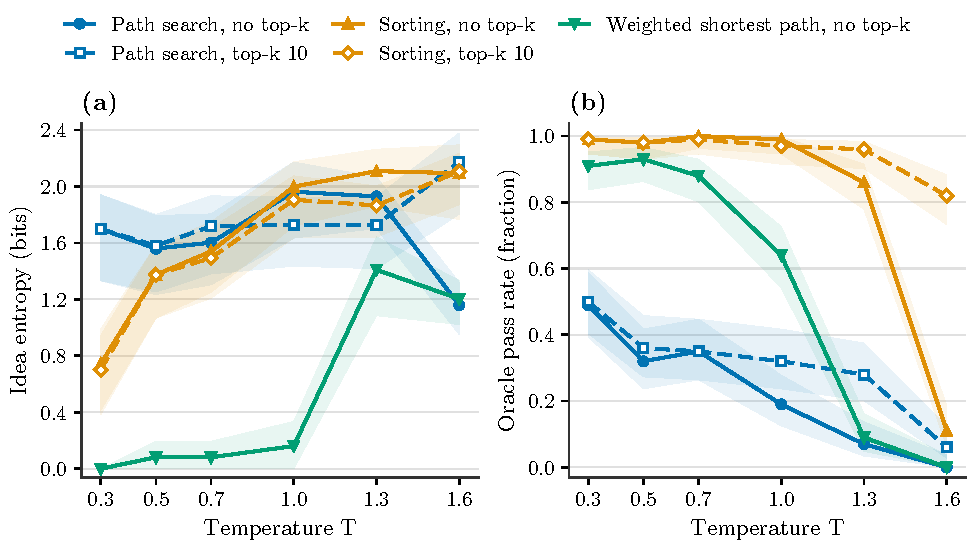
\includegraphics[width=\linewidth,height=0.85\textheight,keepaspectratio]{figures/fig_temp_bare_v0.pdf}
\caption{Temperature re-draw on the bare prompt (Qwen2.5-3B-Instruct, $n = 100$ programs per point, 1,536-token cap, seeds 1000..1099). (a) Idea entropy (bits) and (b) pass rate under the execution oracle, against sampling temperature $T$. Colour encodes the task: blue, path search; amber, sorting; green, weighted shortest path. Solid lines with filled markers use no top-k truncation. Dashed lines with open markers use top-k $= 10$, run for path search and sorting only. Shaded bands are 95\% intervals: percentile bootstrap (2,000 resamples) for entropy and Wilson for pass rate. At $T = 1.6$ without top-k, more than half of the outputs are unparseable, and that class is counted in the entropy, which is why path-search entropy falls there. From $T = 0.3$ to $1.0$, path-search entropy rises by about 0.26 bits while its pass rate falls from 0.49 to 0.19. Sorting gains 1.26 bits at a pass rate of 0.99. The weighted task stays almost entirely Dijkstra (entropy $\le 0.16$ bits) until $T = 1.3$. Above $T = 1.0$, pass rates collapse for every series except sorting with top-k $= 10$ (0.82 at $T = 1.6$). [Source: artifact gen\_art\_experiment\_4, iteration 2.]}
\label{fig:fig_temp_bare}
\end{figure}

\textbf{Temperature adds ideas slowly and breaks code fast.} On path search (re-draw, no top-k), idea entropy rises from 1.70 bits at T = 0.3 to 1.96 at T = 1.0, while the pass rate falls from 0.49 to 0.19. At T = 1.3 a third of outputs are "other" and 65\% hit the token cap, and at T = 1.6 almost nothing parses. Top-k = 10 keeps T = 1.6 parseable and adds a few rare ideas (9 classes on path search), but at a pass rate of 0.06 on path search (0.82 on sorting). Sorting is the one task where heat buys ideas at little cost: entropy rises from 0.74 bits at T = 0.3 to 2.00 at T = 1.0 at pass 0.99. Even there, the new mass goes to the same five comparison sorts. The weighted task stays at Dijkstra up to T = 1.0, and above that the extra entropy comes from broken output, not from new algorithms.

\textbf{The temperature law fails as stated.} Table 39 gives every fitted line of idea log-odds against 1/T, and Table 40 the multinomial-logit fits with a curvature test. Table 41 applies the pre-registered criteria. No task-and-top-k combination meets all of them, on either draw. Three findings matter more than the binary verdict.

First, R\ensuremath{^2} \ensuremath{\geq} 0.85 is a weak criterion at n = 100 per cell. A simulation from a truly linear law with the observed shares gives R\ensuremath{^2} below 0.85 in 25\% to 87\% of draws (Table 42). The curvature likelihood-ratio test is the better check. It does not reject linearity on the grid for path search (p 0.97 and 0.97) and rejects it weakly for sorting without top-k (p 0.034). On the re-draw it rejects linearity only for path search without top-k (p 0.016).

Second, the path-search intercepts are significantly below zero, for example A* at \ensuremath{-}2.38 [\ensuremath{-}3.19, \ensuremath{-}1.56] on the grid. A pure temperature-scaling model, in which each idea has a fixed utility and T only divides the utilities, predicts zero intercepts. Some ideas therefore lose ground at every temperature for reasons that 1/T does not capture. Lines for A* and, on the re-draw, Dijkstra are flat in 1/T: their share relative to BFS does not change with temperature.

Third, rank reversals among the top three occur at T \ensuremath{\leq} 1.3, but only among the minority ideas (A* against DFS on the path-search grid; DFS against Dijkstra on the re-draw; quicksort against bubble sort at T = 1.3 on the sorting grid, not significant). The mode changes only once below T = 1.6: on the sorting grid with top-k 10 at T = 1.3, bubble sort (40) edges past quicksort (37), within noise.

\begingroup\scriptsize
\setlength{\tabcolsep}{2.0pt}
\begin{longtable}{@{}>{\raggedright\arraybackslash\hspace{0pt}}p{37.98pt}>{\raggedright\arraybackslash\hspace{0pt}}p{57.77pt}>{\raggedright\arraybackslash\hspace{0pt}}p{51.32pt}>{\raggedright\arraybackslash\hspace{0pt}}p{57.80pt}>{\raggedright\arraybackslash\hspace{0pt}}p{43.30pt}>{\raggedright\arraybackslash\hspace{0pt}}p{57.83pt}>{\raggedright\arraybackslash\hspace{0pt}}p{29.21pt}>{\raggedright\arraybackslash\hspace{0pt}}p{102.53pt}@{}}
\caption{Fitted lines of idea log-odds (against the modal idea) versus 1/T, weighted least squares, on the grid and the re-draw. "Rest (pooled)" pools all other classes including unparseable output and is not part of the criteria. [Source: artifact gen\_art\_experiment\_4, iteration 2.]}\label{tab:39}\\
\toprule
\textbf{draw} & \textbf{task, top-k} & \textbf{reference (mode)} & \textbf{idea} & \textbf{slope vs 1/T (SE)} & \textbf{intercept (SE)} & \textbf{R\ensuremath{^2}} & \textbf{counts at T = 0.3, 0.5, 0.7, 1.0, 1.3, 1.6 (reference counts)} \\
\midrule
\endfirsthead
\multicolumn{8}{@{}l}{\emph{(continued)}}\\
\toprule
\textbf{draw} & \textbf{task, top-k} & \textbf{reference (mode)} & \textbf{idea} & \textbf{slope vs 1/T (SE)} & \textbf{intercept (SE)} & \textbf{R\ensuremath{^2}} & \textbf{counts at T = 0.3, 0.5, 0.7, 1.0, 1.3, 1.6 (reference counts)} \\
\midrule
\endhead
\bottomrule
\endlastfoot
grid & open path search, none & BFS & DFS & -0.60 (0.18) & -0.73 (0.31) & 0.725 & 5, 12, 10, 15, 12, 2 (82, 73, 72, 54, 44, 1) \\
grid & open path search, none & BFS & Dijkstra & -0.77 (0.22) & -0.89 (0.34) & 0.760 & 2, 7, 7, 12, 7, 1 (82, 73, 72, 54, 44, 1) \\
grid & open path search, none & BFS & A* & -0.09 (0.22) & -1.99 (0.47) & 0.035 & 9, 5, 7, 10, 1, 0 (82, 73, 72, 54, 44, 1) \\
grid & open path search, none & BFS & rest (pooled) (not eligible) & -1.71 (0.81) & 0.88 (1.08) & 0.523 & 2, 3, 4, 9, 36, 96 (82, 73, 72, 54, 44, 1) \\
grid & open path search, 10 & BFS & A* & -0.08 (0.22) & -1.95 (0.43) & 0.033 & 9, 5, 8, 13, 5, 2 (82, 73, 67, 59, 59, 46) \\
grid & open path search, 10 & BFS & DFS & -0.62 (0.10) & -0.65 (0.15) & 0.908 & 5, 12, 13, 12, 19, 19 (82, 73, 67, 59, 59, 46) \\
grid & open path search, 10 & BFS & Dijkstra & -0.71 (0.06) & -0.99 (0.09) & 0.968 & 2, 7, 8, 11, 11, 11 (82, 73, 67, 59, 59, 46) \\
grid & open path search, 10 & BFS & rest (pooled) (not eligible) & -1.08 (0.42) & -0.65 (0.55) & 0.626 & 2, 3, 4, 5, 6, 22 (82, 73, 67, 59, 59, 46) \\
grid & sorting, none & quicksort & bubble sort & -0.55 (0.07) & 0.26 (0.12) & 0.944 & 18, 23, 34, 32, 35, 18 (80, 68, 55, 45, 37, 20) \\
grid & sorting, none & quicksort & merge sort & -1.04 (0.16) & -0.05 (0.22) & 0.911 & 1, 9, 11, 15, 18, 6 (80, 68, 55, 45, 37, 20) \\
grid & sorting, none & quicksort & selection sort & -1.21 (0.43) & -0.66 (0.54) & 0.661 & 1, 0, 0, 5, 6, 8 (80, 68, 55, 45, 37, 20) \\
grid & sorting, none & quicksort & insertion sort & -1.70 (0.58) & -0.68 (0.65) & 0.683 & 0, 0, 0, 3, 2, 6 (80, 68, 55, 45, 37, 20) \\
grid & sorting, none & quicksort & rest (pooled) (not eligible) & -2.84 (1.33) & 1.91 (1.24) & 0.533 & 0, 0, 0, 0, 2, 42 (80, 68, 55, 45, 37, 20) \\
grid & sorting, 10 & quicksort & bubble sort & -0.60 (0.09) & 0.35 (0.14) & 0.926 & 17, 24, 30, 33, 40, 37 (79, 66, 55, 51, 37, 34) \\
grid & sorting, 10 & quicksort & merge sort & -0.95 (0.15) & -0.14 (0.21) & 0.908 & 2, 9, 14, 11, 16, 18 (79, 66, 55, 51, 37, 34) \\
grid & sorting, 10 & quicksort & insertion sort & -1.19 (0.34) & -1.67 (0.40) & 0.756 & 0, 0, 0, 3, 3, 2 (79, 66, 55, 51, 37, 34) \\
grid & sorting, 10 & quicksort & rest (pooled) (not eligible) & -0.81 (0.36) & -1.34 (0.54) & 0.563 & 2, 1, 1, 2, 4, 9 (79, 66, 55, 51, 37, 34) \\
grid & weighted shortest path, none & Dijkstra & rest (pooled) (not eligible) & -3.27 (1.94) & 2.17 (1.78) & 0.416 & 0, 0, 0, 1, 33, 96 (100, 100, 100, 99, 67, 4) \\
grid & weighted shortest path, 10 & Dijkstra & rest (pooled) (not eligible) & -1.87 (0.85) & -0.77 (0.78) & 0.547 & 0, 0, 0, 0, 3, 17 (100, 100, 100, 100, 97, 83) \\
re-draw & open path search, none & BFS & Dijkstra & -0.08 (0.17) & -1.44 (0.34) & 0.053 & 14, 6, 9, 14, 11, 0 (64, 66, 61, 55, 39, 2) \\
re-draw & open path search, none & BFS & DFS & -0.35 (0.12) & -0.83 (0.21) & 0.696 & 8, 12, 21, 14, 12, 0 (64, 66, 61, 55, 39, 2) \\
re-draw & open path search, none & BFS & A* & 0.07 (0.19) & -2.03 (0.41) & 0.031 & 9, 12, 7, 8, 0, 0 (64, 66, 61, 55, 39, 2) \\
re-draw & open path search, none & BFS & rest (pooled) (not eligible) & -1.20 (0.74) & 0.64 (1.14) & 0.398 & 5, 4, 2, 9, 38, 98 (64, 66, 61, 55, 39, 2) \\
re-draw & open path search, 10 & BFS & DFS & -0.53 (0.12) & -0.51 (0.19) & 0.819 & 8, 9, 16, 18, 21, 26 (64, 65, 61, 59, 58, 47) \\
re-draw & open path search, 10 & BFS & Dijkstra & 0.01 (0.07) & -1.62 (0.12) & 0.002 & 14, 10, 11, 11, 11, 11 (64, 65, 61, 59, 58, 47) \\
re-draw & open path search, 10 & BFS & A* & 0.14 (0.13) & -2.13 (0.24) & 0.227 & 9, 14, 8, 7, 7, 4 (64, 65, 61, 59, 58, 47) \\
re-draw & open path search, 10 & BFS & rest (pooled) (not eligible) & -0.33 (0.29) & -1.75 (0.50) & 0.237 & 5, 2, 4, 5, 3, 12 (64, 65, 61, 59, 58, 47) \\
re-draw & sorting, none & bubble sort & quicksort & -0.90 (0.09) & 0.30 (0.14) & 0.959 & 5, 18, 20, 23, 28, 15 (88, 68, 62, 47, 41, 16) \\
re-draw & sorting, none & bubble sort & merge sort & -0.75 (0.11) & -0.41 (0.17) & 0.920 & 4, 10, 13, 18, 14, 4 (88, 68, 62, 47, 41, 16) \\
re-draw & sorting, none & bubble sort & selection sort & -0.62 (0.18) & -1.61 (0.30) & 0.743 & 2, 3, 3, 7, 4, 1 (88, 68, 62, 47, 41, 16) \\
re-draw & sorting, none & bubble sort & insertion sort & -1.10 (0.37) & -1.01 (0.52) & 0.688 & 1, 1, 2, 3, 10, 1 (88, 68, 62, 47, 41, 16) \\
re-draw & sorting, none & bubble sort & rest (pooled) (not eligible) & -3.29 (1.65) & 2.44 (1.55) & 0.499 & 0, 0, 0, 2, 3, 63 (88, 68, 62, 47, 41, 16) \\
re-draw & sorting, 10 & bubble sort & quicksort & -1.02 (0.10) & 0.54 (0.14) & 0.965 & 4, 18, 20, 31, 32, 32 (89, 68, 63, 46, 42, 35) \\
re-draw & sorting, 10 & bubble sort & merge sort & -0.83 (0.08) & -0.28 (0.11) & 0.968 & 4, 10, 13, 12, 18, 17 (89, 68, 63, 46, 42, 35) \\
re-draw & sorting, 10 & bubble sort & selection sort & -0.90 (0.27) & -1.04 (0.40) & 0.729 & 2, 3, 2, 5, 5, 11 (89, 68, 63, 46, 42, 35) \\
re-draw & sorting, 10 & bubble sort & insertion sort & -0.78 (0.21) & -1.75 (0.30) & 0.778 & 1, 1, 2, 5, 3, 3 (89, 68, 63, 46, 42, 35) \\
re-draw & sorting, 10 & bubble sort & rest (pooled) (not eligible) & -0.99 (0.37) & -2.46 (0.51) & 0.645 & 0, 0, 0, 1, 0, 2 (89, 68, 63, 46, 42, 35) \\
re-draw & weighted shortest path, none & Dijkstra & rest (pooled) (not eligible) & -3.40 (1.66) & 2.38 (1.61) & 0.514 & 0, 1, 1, 2, 37, 95 (100, 99, 99, 98, 63, 5) \\
\end{longtable}
\endgroup
\begingroup\footnotesize
\setlength{\tabcolsep}{3.0pt}
\begin{longtable}{@{}>{\raggedright\arraybackslash\hspace{0pt}}p{45.35pt}>{\raggedright\arraybackslash\hspace{0pt}}p{70.32pt}>{\raggedright\arraybackslash\hspace{0pt}}p{88.25pt}>{\raggedright\arraybackslash\hspace{0pt}}p{60.22pt}>{\raggedright\arraybackslash\hspace{0pt}}p{97.12pt}>{\raggedright\arraybackslash\hspace{0pt}}p{72.50pt}@{}}
\caption{Multinomial-logit fits with a curvature likelihood-ratio test (linear vs quadratic in 1/T). [Source: artifact gen\_art\_experiment\_4, iteration 2.]}\label{tab:40}\\
\toprule
\textbf{draw} & \textbf{task, top-k} & \textbf{curvature likelihood-ratio test (df), p} & \textbf{idea} & \textbf{intercept [95\% CI], p} & \textbf{slope [95\% CI]} \\
\midrule
\endfirsthead
\multicolumn{6}{@{}l}{\emph{(continued)}}\\
\toprule
\textbf{draw} & \textbf{task, top-k} & \textbf{curvature likelihood-ratio test (df), p} & \textbf{idea} & \textbf{intercept [95\% CI], p} & \textbf{slope [95\% CI]} \\
\midrule
\endhead
\bottomrule
\endlastfoot
grid & open path search, none & 0.22 (3), 0.975 & DFS & -0.76 [-1.39, -0.12], 0.019 & -0.61 [-1.00, -0.23] \\
grid & open path search, none & 0.22 (3), 0.975 & Dijkstra & -0.96 [-1.74, -0.17], 0.017 & -0.79 [-1.30, -0.28] \\
grid & open path search, none & 0.22 (3), 0.975 & A* & -2.38 [-3.19, -1.56], 1e-08 & 0.03 [-0.35, 0.41] \\
grid & open path search, 10 & 0.27 (3), 0.966 & A* & -2.18 [-2.81, -1.54], 1.8e-11 & -0.03 [-0.36, 0.31] \\
grid & open path search, 10 & 0.27 (3), 0.966 & DFS & -0.66 [-1.14, -0.17], 0.0086 & -0.64 [-0.98, -0.31] \\
grid & open path search, 10 & 0.27 (3), 0.966 & Dijkstra & -0.99 [-1.60, -0.38], 0.0014 & -0.76 [-1.20, -0.32] \\
grid & sorting, none & 10.41 (4), 0.034 & bubble sort & 0.26 [-0.14, 0.66], 0.2 & -0.56 [-0.79, -0.33] \\
grid & sorting, none & 10.41 (4), 0.034 & merge sort & -0.07 [-0.69, 0.54], 0.82 & -1.07 [-1.52, -0.62] \\
grid & sorting, none & 10.41 (4), 0.034 & selection sort & 0.18 [-1.17, 1.53], 0.8 & -2.41 [-3.80, -1.03] \\
grid & sorting, none & 10.41 (4), 0.034 & insertion sort & 1.79 [-1.07, 4.65], 0.22 & -5.15 [-8.82, -1.47] \\
grid & sorting, 10 & 4.77 (3), 0.189 & bubble sort & 0.36 [-0.01, 0.73], 0.056 & -0.62 [-0.84, -0.39] \\
grid & sorting, 10 & 4.77 (3), 0.189 & merge sort & -0.17 [-0.72, 0.38], 0.54 & -0.96 [-1.37, -0.56] \\
grid & sorting, 10 & 4.77 (3), 0.189 & insertion sort & -0.66 [-2.89, 1.56], 0.56 & -2.76 [-5.32, -0.20] \\
re-draw & open path search, none & 10.27 (3), 0.016 & Dijkstra & -1.53 [-2.16, -0.89], 2.7e-06 & -0.08 [-0.41, 0.24] \\
re-draw & open path search, none & 10.27 (3), 0.016 & DFS & -0.88 [-1.46, -0.29], 0.0032 & -0.35 [-0.67, -0.02] \\
re-draw & open path search, none & 10.27 (3), 0.016 & A* & -2.49 [-3.28, -1.69], 7.8e-10 & 0.22 [-0.15, 0.58] \\
re-draw & open path search, 10 & 5.41 (3), 0.144 & DFS & -0.50 [-0.95, -0.05], 0.029 & -0.57 [-0.88, -0.26] \\
re-draw & open path search, 10 & 5.41 (3), 0.144 & Dijkstra & -1.66 [-2.17, -1.15], 1.5e-10 & 0.01 [-0.27, 0.28] \\
re-draw & open path search, 10 & 5.41 (3), 0.144 & A* & -2.20 [-2.80, -1.61], 4.4e-13 & 0.14 [-0.17, 0.44] \\
re-draw & sorting, none & 2.22 (4), 0.695 & quicksort & 0.33 [-0.16, 0.81], 0.19 & -0.93 [-1.25, -0.61] \\
re-draw & sorting, none & 2.22 (4), 0.695 & merge sort & -0.44 [-1.02, 0.13], 0.13 & -0.76 [-1.12, -0.39] \\
re-draw & sorting, none & 2.22 (4), 0.695 & selection sort & -1.75 [-2.69, -0.80], 0.00029 & -0.64 [-1.23, -0.05] \\
re-draw & sorting, none & 2.22 (4), 0.695 & insertion sort & -0.93 [-2.07, 0.21], 0.11 & -1.40 [-2.34, -0.47] \\
re-draw & sorting, 10 & 3.67 (4), 0.453 & quicksort & 0.53 [0.10, 0.96], 0.015 & -1.03 [-1.33, -0.72] \\
re-draw & sorting, 10 & 3.67 (4), 0.453 & merge sort & -0.29 [-0.81, 0.23], 0.27 & -0.85 [-1.21, -0.49] \\
re-draw & sorting, 10 & 3.67 (4), 0.453 & selection sort & -1.04 [-1.86, -0.23], 0.012 & -1.04 [-1.67, -0.41] \\
re-draw & sorting, 10 & 3.67 (4), 0.453 & insertion sort & -1.79 [-2.86, -0.72], 0.001 & -0.93 [-1.73, -0.14] \\
\end{longtable}
\endgroup
\begingroup\scriptsize
\setlength{\tabcolsep}{2.0pt}
\begin{longtable}{@{}>{\raggedright\arraybackslash\hspace{0pt}}p{37.18pt}>{\raggedright\arraybackslash\hspace{0pt}}p{58.71pt}>{\raggedright\arraybackslash\hspace{0pt}}p{98.13pt}>{\raggedright\arraybackslash\hspace{0pt}}p{22.60pt}>{\raggedright\arraybackslash\hspace{0pt}}p{79.23pt}>{\raggedright\arraybackslash\hspace{0pt}}p{51.32pt}>{\raggedright\arraybackslash\hspace{0pt}}p{46.64pt}>{\raggedright\arraybackslash\hspace{0pt}}p{43.95pt}@{}}
\caption{Pre-registered criteria of the temperature law, per draw and task. The within/between slope ratio compares the slope of ln alpha\_1 with the slope of ln beta\_1 against T; the law requires at least 3. [Source: artifact gen\_art\_experiment\_4, iteration 2.]}\label{tab:41}\\
\toprule
\textbf{draw} & \textbf{task, top-k} & \textbf{R\ensuremath{^2} per eligible line} & \textbf{all R\ensuremath{^2} \textgreater{}= 0.85} & \textbf{top-3 rank reversals at T \textless{}= 1.3} & \textbf{within/between slope ratio [95\% CI]} & \textbf{curvature p} & \textbf{criterion met} \\
\midrule
\endfirsthead
\multicolumn{8}{@{}l}{\emph{(continued)}}\\
\toprule
\textbf{draw} & \textbf{task, top-k} & \textbf{R\ensuremath{^2} per eligible line} & \textbf{all R\ensuremath{^2} \textgreater{}= 0.85} & \textbf{top-3 rank reversals at T \textless{}= 1.3} & \textbf{within/between slope ratio [95\% CI]} & \textbf{curvature p} & \textbf{criterion met} \\
\midrule
\endhead
\bottomrule
\endlastfoot
grid & open path search, none & DFS 0.72, Dijkstra 0.76, A* 0.03 & no & none & 1.15 [0.74, 1.76] & 0.975 & no \\
grid & open path search, 10 & A* 0.03, DFS 0.91, Dijkstra 0.97 & no & T=0.5: DFS above A* (0.12 vs 0.05, one-sided p\textless{}0.05); T=0.7: DFS above A* (0.13 vs 0.08); T=1.3: DFS above A* (0.19 vs 0.05, one-sided p\textless{}0.05) & 1.05 [0.68, 1.36] & 0.966 & no \\
grid & sorting, none & bubble sort 0.94, merge sort 0.91, selection sort 0.66, insertion sort 0.68 & no & none & 0.58 [0.46, 0.72] & 0.034 & no \\
grid & sorting, 10 & bubble sort 0.93, merge sort 0.91, insertion sort 0.76 & no & T=1.3: bubble sort above quicksort (0.40 vs 0.37) & 0.73 [0.55, 1.01] & 0.189 & no \\
grid & weighted shortest path, none & not eligible: fewer than 2 ideas at 3\% or more at T = 1 &  &  &  &  &  \\
grid & weighted shortest path, 10 & not eligible: fewer than 2 ideas at 3\% or more at T = 1 &  &  &  &  &  \\
re-draw & open path search, none & Dijkstra 0.05, DFS 0.70, A* 0.03 & no & T=0.3: Dijkstra above DFS (0.14 vs 0.08) & 2.64 [1.27, 9.49] & 0.016 & no \\
re-draw & open path search, 10 & DFS 0.82, Dijkstra 0.00, A* 0.23 & no & T=0.3: Dijkstra above DFS (0.14 vs 0.08); T=0.5: Dijkstra above DFS (0.10 vs 0.09) & 2.23 [1.12, 8.43] & 0.144 & no \\
re-draw & sorting, none & quicksort 0.96, merge sort 0.92, selection sort 0.74, insertion sort 0.69 & no & none & 0.79 [0.54, 1.03] & 0.695 & no \\
re-draw & sorting, 10 & quicksort 0.97, merge sort 0.97, selection sort 0.73, insertion sort 0.78 & no & none & 0.68 [0.50, 0.86] & 0.453 & no \\
re-draw & weighted shortest path, none & not eligible: fewer than 2 ideas at 3\% or more at T = 1 &  &  &  &  &  \\
\end{longtable}
\endgroup
\begingroup\small
\setlength{\tabcolsep}{4.0pt}
\begin{longtable}{@{}>{\raggedright\arraybackslash\hspace{0pt}}p{102.92pt}>{\raggedright\arraybackslash\hspace{0pt}}p{247.49pt}>{\raggedright\arraybackslash\hspace{0pt}}p{95.34pt}@{}}
\caption{Simulation under a true linear law with the observed shares (200 simulated grids per line): how often R\ensuremath{^2} falls below 0.85, and how often the curvature test falsely rejects. [Source: artifact gen\_art\_experiment\_4, iteration 2.]}\label{tab:42}\\
\toprule
\textbf{task, top-k} & \textbf{share of simulated draws with R\ensuremath{^2} \textless{} 0.85 under a true linear law, per idea} & \textbf{curvature test false-rejection rate} \\
\midrule
\endfirsthead
\multicolumn{3}{@{}l}{\emph{(continued)}}\\
\toprule
\textbf{task, top-k} & \textbf{share of simulated draws with R\ensuremath{^2} \textless{} 0.85 under a true linear law, per idea} & \textbf{curvature test false-rejection rate} \\
\midrule
\endhead
\bottomrule
\endlastfoot
open path search, none & DFS 0.275, Dijkstra 0.350, A* 0.365 & 0.085 \\
open path search, 10 & A* 0.295, DFS 0.250, Dijkstra 0.265 & 0.045 \\
sorting, none & bubble sort 0.710, merge sort 0.370, selection sort 0.615, insertion sort 0.865 & 0.070 \\
sorting, 10 & bubble sort 0.600, merge sort 0.410, insertion sort 0.810 & 0.095 \\
\end{longtable}
\endgroup
\textbf{Ideas against phrasings: the answer to questions (a), (b) and (c) of the original request.} Table 43 gives the diversity partition and Table 44 the "10 trajectories" view. At T = 0.3 on the open task, 10 programs contain about 2.4 (grid) to 3.5 (re-draw) distinct ideas and 8.3 to 9.1 distinct phrasings (normalised code at edit-distance similarity below 0.85). The model gives a few ideas, each in many phrasings, even at the tightest temperature; that is the user's case (a). Case (b), ten ideas with one phrasing each, never occurs: the largest expected number of ideas among 10 in any cell is 4.9 (sorting, T = 1.6, no top-k, where a third of outputs are unparseable). As T rises the number of ideas grows slowly (path-search re-draw: 3.5 to 3.9 from T = 0.3 to 1.0) and phrasings saturate at 10 of 10 by T = 1.0. Sorting differs. At T = 0.3 the sorting programs are written almost identically every time (2.4 to 2.8 distinct phrasings among 10), and heat adds both ideas and phrasings, with between-idea diversity rising faster than within-idea diversity (slope ratio 0.58 to 0.79). Phrasing grows at least 3 times faster than ideas in no cell; the largest ratio is 2.64, on the path-search re-draw.

\begingroup\footnotesize
\setlength{\tabcolsep}{3.0pt}
\begin{longtable}{@{}>{\raggedright\arraybackslash\hspace{0pt}}p{41.85pt}>{\raggedright\arraybackslash\hspace{0pt}}p{66.39pt}>{\raggedright\arraybackslash\hspace{0pt}}p{86.12pt}>{\raggedright\arraybackslash\hspace{0pt}}p{79.15pt}>{\raggedright\arraybackslash\hspace{0pt}}p{63.23pt}>{\raggedright\arraybackslash\hspace{0pt}}p{58.25pt}>{\raggedright\arraybackslash\hspace{0pt}}p{32.75pt}@{}}
\caption{Diversity partition: log within-idea (alpha\_1) and log between-idea (beta\_1) diversity per temperature, with slopes against T. [Source: artifact gen\_art\_experiment\_4, iteration 2.]}\label{tab:43}\\
\toprule
\textbf{draw} & \textbf{task, top-k} & \textbf{ln alpha\_1 at T = 0.3, 0.5, 0.7, 1.0, 1.3, 1.6} & \textbf{ln beta\_1 at the same T} & \textbf{slope of ln alpha\_1 [95\% CI]} & \textbf{slope of ln beta\_1 [95\% CI]} & \textbf{ratio} \\
\midrule
\endfirsthead
\multicolumn{7}{@{}l}{\emph{(continued)}}\\
\toprule
\textbf{draw} & \textbf{task, top-k} & \textbf{ln alpha\_1 at T = 0.3, 0.5, 0.7, 1.0, 1.3, 1.6} & \textbf{ln beta\_1 at the same T} & \textbf{slope of ln alpha\_1 [95\% CI]} & \textbf{slope of ln beta\_1 [95\% CI]} & \textbf{ratio} \\
\midrule
\endhead
\bottomrule
\endlastfoot
grid & open path search, none & 0.52, 0.70, 0.80, 1.03, 1.17, n/a & 0.70, 0.94, 0.97, 1.35, 1.22, 0.47 & 0.65 [0.50, 0.69] & 0.56 [0.34, 0.76] & 1.15 \\
grid & open path search, 10 & 0.52, 0.68, 0.86, 0.99, 1.14, 1.25 & 0.70, 0.94, 1.07, 1.25, 1.22, 1.49 & 0.56 [0.43, 0.57] & 0.53 [0.37, 0.70] & 1.05 \\
grid & sorting, none & 0.03, 0.19, 0.27, 0.32, 0.47, 0.75 & 0.58, 0.82, 0.94, 1.26, 1.38, 1.74 & 0.49 [0.38, 0.54] & 0.85 [0.67, 0.96] & 0.58 \\
grid & sorting, 10 & 0.02, 0.12, 0.27, 0.32, 0.43, 0.52 & 0.64, 0.88, 1.01, 1.14, 1.26, 1.34 & 0.37 [0.31, 0.43] & 0.50 [0.36, 0.64] & 0.73 \\
grid & weighted shortest path, none & 0.36, 0.48, 0.54, 0.79, 1.16, n/a & 0.00, 0.00, 0.00, 0.06, 0.67, 0.30 & 0.78 [0.66, 0.85] & 0.59 [0.48, 0.68] & 1.31 \\
grid & weighted shortest path, 10 & 0.37, 0.47, 0.53, 0.75, 1.07, 1.20 & 0.00, 0.00, 0.00, 0.00, 0.15, 0.68 & 0.67 [0.59, 0.70] & 0.44 [0.28, 0.55] & 1.52 \\
re-draw & open path search, none & 0.58, 0.74, 0.84, 1.08, 1.24, n/a & 1.18, 1.08, 1.11, 1.36, 1.34, 0.31 & 0.66 [0.48, 0.70] & 0.25 [0.05, 0.46] & 2.64 \\
re-draw & open path search, 10 & 0.59, 0.72, 0.83, 0.99, 1.09, 1.25 & 1.18, 1.09, 1.19, 1.20, 1.20, 1.51 & 0.50 [0.39, 0.53] & 0.22 [0.05, 0.39] & 2.23 \\
re-draw & sorting, none & 0.08, 0.10, 0.20, 0.28, 0.51, 0.88 & 0.52, 0.95, 1.07, 1.38, 1.46, 1.55 & 0.59 [0.42, 0.61] & 0.74 [0.53, 0.86] & 0.79 \\
re-draw & sorting, 10 & 0.08, 0.10, 0.21, 0.27, 0.42, 0.67 & 0.49, 0.95, 1.03, 1.32, 1.29, 1.46 & 0.44 [0.36, 0.47] & 0.65 [0.49, 0.81] & 0.68 \\
re-draw & weighted shortest path, none & 0.36, 0.43, 0.49, 0.86, 1.18, n/a & 0.00, 0.06, 0.06, 0.11, 0.93, 0.37 & 0.85 [0.71, 0.88] & 0.81 [0.62, 0.94] & 1.06 \\
\end{longtable}
\endgroup
\begingroup\footnotesize
\setlength{\tabcolsep}{3.0pt}
\begin{longtable}{@{}>{\raggedright\arraybackslash\hspace{0pt}}p{50.57pt}>{\raggedright\arraybackslash\hspace{0pt}}p{94.51pt}>{\raggedright\arraybackslash\hspace{0pt}}p{44.86pt}>{\raggedright\arraybackslash\hspace{0pt}}p{55.36pt}>{\raggedright\arraybackslash\hspace{0pt}}p{58.66pt}>{\raggedright\arraybackslash\hspace{0pt}}p{59.66pt}>{\raggedright\arraybackslash\hspace{0pt}}p{64.12pt}@{}}
\caption{The user's "10 trajectories" view: expected distinct ideas and distinct phrasings in a random draw of 10 programs. A cell is labelled (a) when it has at most 3 ideas and at least 7 phrasings, (b) when it has at least 7 ideas, and mixed otherwise. The last row of each block is the change from T = 0.3 to 1.3 with the verdict for the user's case (c). [Source: artifact gen\_art\_experiment\_4, iteration 2.]}\label{tab:44}\\
\toprule
\textbf{draw} & \textbf{task, top-k} & \textbf{T} & \textbf{expected distinct ideas among 10} & \textbf{expected distinct phrasings among 10} & \textbf{phrasings per idea} & \textbf{cell verdict} \\
\midrule
\endfirsthead
\multicolumn{7}{@{}l}{\emph{(continued)}}\\
\toprule
\textbf{draw} & \textbf{task, top-k} & \textbf{T} & \textbf{expected distinct ideas among 10} & \textbf{expected distinct phrasings among 10} & \textbf{phrasings per idea} & \textbf{cell verdict} \\
\midrule
\endhead
\bottomrule
\endlastfoot
grid & open path search, none & 0.3 & 2.44 & 8.34 & 3.42 & (a) \\
grid & open path search, none & 0.5 & 2.98 & 9.51 & 3.19 & (a) \\
grid & open path search, none & 0.7 & 3.08 & 9.89 & 3.21 & mixed \\
grid & open path search, none & 1.0 & 3.91 & 10.00 & 2.56 & mixed \\
grid & open path search, none & 1.3 & 3.46 & 10.00 & 2.89 & mixed \\
grid & open path search, none & 1.6 & 2.37 & 4.27 & 1.80 & mixed \\
grid & open path search, none & change 0.3 to 1.3 & +1.02 &  & -0.53 & neither \\
grid & open path search, 10 & 0.3 & 2.44 & 8.30 & 3.41 & (a) \\
grid & open path search, 10 & 0.5 & 2.98 & 9.46 & 3.17 & (a) \\
grid & open path search, 10 & 0.7 & 3.28 & 9.90 & 3.02 & mixed \\
grid & open path search, 10 & 1.0 & 3.66 & 10.00 & 2.73 & mixed \\
grid & open path search, 10 & 1.3 & 3.53 & 10.00 & 2.83 & mixed \\
grid & open path search, 10 & 1.6 & 4.17 & 10.00 & 2.40 & mixed \\
grid & open path search, 10 & change 0.3 to 1.3 & +1.09 &  & -0.58 & neither \\
grid & sorting, none & 0.3 & 2.08 & 2.35 & 1.13 & mixed \\
grid & sorting, none & 0.5 & 2.57 & 3.73 & 1.45 & mixed \\
grid & sorting, none & 0.7 & 2.69 & 4.82 & 1.79 & mixed \\
grid & sorting, none & 1.0 & 3.49 & 7.17 & 2.06 & mixed \\
grid & sorting, none & 1.3 & 3.73 & 8.16 & 2.19 & mixed \\
grid & sorting, none & 1.6 & 4.93 & 7.23 & 1.47 & mixed \\
grid & sorting, none & change 0.3 to 1.3 & +1.65 &  & +1.06 & c-b (more ideas) \\
grid & sorting, 10 & 0.3 & 2.24 & 2.58 & 1.15 & mixed \\
grid & sorting, 10 & 0.5 & 2.67 & 3.56 & 1.33 & mixed \\
grid & sorting, 10 & 0.7 & 2.87 & 5.16 & 1.80 & mixed \\
grid & sorting, 10 & 1.0 & 3.16 & 6.53 & 2.07 & mixed \\
grid & sorting, 10 & 1.3 & 3.45 & 7.96 & 2.31 & mixed \\
grid & sorting, 10 & 1.6 & 3.68 & 9.02 & 2.45 & mixed \\
grid & sorting, 10 & change 0.3 to 1.3 & +1.21 &  & +1.16 & c-a (few ideas, more phrasings each) \\
grid & weighted shortest path, none & 0.3 & 1.00 & 7.04 & 7.04 & (a) \\
grid & weighted shortest path, none & 0.5 & 1.00 & 8.78 & 8.78 & (a) \\
grid & weighted shortest path, none & 0.7 & 1.00 & 9.06 & 9.06 & (a) \\
grid & weighted shortest path, none & 1.0 & 1.10 & 9.81 & 8.92 & (a) \\
grid & weighted shortest path, none & 1.3 & 2.27 & 9.98 & 4.40 & (a) \\
grid & weighted shortest path, none & 1.6 & 2.34 & 5.49 & 2.34 & mixed \\
grid & weighted shortest path, none & change 0.3 to 1.3 & +1.27 &  & -2.63 & neither \\
grid & weighted shortest path, 10 & 0.3 & 1.00 & 6.94 & 6.94 & mixed \\
grid & weighted shortest path, 10 & 0.5 & 1.00 & 8.78 & 8.78 & (a) \\
grid & weighted shortest path, 10 & 0.7 & 1.00 & 8.88 & 8.88 & (a) \\
grid & weighted shortest path, 10 & 1.0 & 1.00 & 9.86 & 9.86 & (a) \\
grid & weighted shortest path, 10 & 1.3 & 1.29 & 9.99 & 7.74 & (a) \\
grid & weighted shortest path, 10 & 1.6 & 2.38 & 10.00 & 4.21 & (a) \\
grid & weighted shortest path, 10 & change 0.3 to 1.3 & +0.29 &  & +0.80 & c-a (few ideas, more phrasings each) \\
re-draw & open path search, none & 0.3 & 3.48 & 9.10 & 2.61 & mixed \\
re-draw & open path search, none & 0.5 & 3.30 & 9.76 & 2.95 & mixed \\
re-draw & open path search, none & 0.7 & 3.27 & 9.85 & 3.01 & mixed \\
re-draw & open path search, none & 1.0 & 3.91 & 10.00 & 2.56 & mixed \\
re-draw & open path search, none & 1.3 & 3.70 & 10.00 & 2.70 & mixed \\
re-draw & open path search, none & 1.6 & 2.28 & 4.90 & 2.14 & mixed \\
re-draw & open path search, none & change 0.3 to 1.3 & +0.22 &  & +0.09 & c-a (few ideas, more phrasings each) \\
re-draw & open path search, 10 & 0.3 & 3.48 & 9.18 & 2.64 & mixed \\
re-draw & open path search, 10 & 0.5 & 3.29 & 9.32 & 2.83 & mixed \\
re-draw & open path search, 10 & 0.7 & 3.50 & 9.89 & 2.82 & mixed \\
re-draw & open path search, 10 & 1.0 & 3.53 & 10.00 & 2.83 & mixed \\
re-draw & open path search, 10 & 1.3 & 3.45 & 10.00 & 2.90 & mixed \\
re-draw & open path search, 10 & 1.6 & 4.11 & 10.00 & 2.43 & mixed \\
re-draw & open path search, 10 & change 0.3 to 1.3 & -0.03 &  & +0.27 & c-a (few ideas, more phrasings each) \\
re-draw & sorting, none & 0.3 & 2.06 & 2.82 & 1.37 & mixed \\
re-draw & sorting, none & 0.5 & 2.92 & 3.99 & 1.37 & mixed \\
re-draw & sorting, none & 0.7 & 3.14 & 4.83 & 1.54 & mixed \\
re-draw & sorting, none & 1.0 & 3.82 & 5.91 & 1.55 & mixed \\
re-draw & sorting, none & 1.3 & 4.05 & 8.68 & 2.14 & mixed \\
re-draw & sorting, none & 1.6 & 4.07 & 5.89 & 1.45 & mixed \\
re-draw & sorting, none & change 0.3 to 1.3 & +2.00 &  & +0.77 & c-b (more ideas) \\
re-draw & sorting, 10 & 0.3 & 1.99 & 2.69 & 1.36 & mixed \\
re-draw & sorting, 10 & 0.5 & 2.92 & 4.03 & 1.38 & mixed \\
re-draw & sorting, 10 & 0.7 & 3.06 & 4.85 & 1.59 & mixed \\
re-draw & sorting, 10 & 1.0 & 3.65 & 6.22 & 1.70 & mixed \\
re-draw & sorting, 10 & 1.3 & 3.55 & 7.85 & 2.21 & mixed \\
re-draw & sorting, 10 & 1.6 & 4.00 & 9.36 & 2.34 & mixed \\
re-draw & sorting, 10 & change 0.3 to 1.3 & +1.56 &  & +0.86 & c-b (more ideas) \\
re-draw & weighted shortest path, none & 0.3 & 1.00 & 6.55 & 6.55 & mixed \\
re-draw & weighted shortest path, none & 0.5 & 1.10 & 7.36 & 6.69 & (a) \\
re-draw & weighted shortest path, none & 0.7 & 1.10 & 8.21 & 7.46 & (a) \\
re-draw & weighted shortest path, none & 1.0 & 1.20 & 9.96 & 8.30 & (a) \\
re-draw & weighted shortest path, none & 1.3 & 2.75 & 10.00 & 3.64 & (a) \\
re-draw & weighted shortest path, none & 1.6 & 2.41 & 4.82 & 2.00 & mixed \\
re-draw & weighted shortest path, none & change 0.3 to 1.3 & +1.75 &  & -2.91 & c-b (more ideas) \\
\end{longtable}
\endgroup
\textbf{Out of sample, the frozen law helps on path search and hurts on sorting.} Table 45 scores the frozen grid fits on the re-draw against two baselines. One is fixed utilities, in which the T = 0.7 shares are raised to the power 0.7/T. The other is no temperature effect at all. On path search with top-k 10 the frozen law has a mean absolute error of 0.040 against 0.073 for fixed utilities, and without top-k 0.109 against 0.129. On sorting it loses (0.100 and 0.103 against 0.028 and 0.056). The sorting loss is largely the wording change: the grid was fitted with quicksort as the mode and the re-draw has bubble sort as the mode, so the frozen ordering is reversed at every temperature.

\begingroup\footnotesize
\setlength{\tabcolsep}{3.0pt}
\begin{longtable}{@{}>{\raggedright\arraybackslash\hspace{0pt}}p{42.42pt}>{\raggedright\arraybackslash\hspace{0pt}}p{65.74pt}>{\raggedright\arraybackslash\hspace{0pt}}p{54.57pt}>{\raggedright\arraybackslash\hspace{0pt}}p{46.86pt}>{\raggedright\arraybackslash\hspace{0pt}}p{64.80pt}>{\raggedright\arraybackslash\hspace{0pt}}p{60.94pt}>{\raggedright\arraybackslash\hspace{0pt}}p{92.42pt}@{}}
\caption{Out-of-sample scoring of the frozen temperature law on the re-draw (mean absolute error over ideas and temperatures, calibration slope in brackets, and mean JSD per cell). [Source: artifact gen\_art\_experiment\_4, iteration 2.]}\label{tab:45}\\
\toprule
\textbf{task, top-k} & \textbf{frozen law, anchored: MAE (calibration slope)} & \textbf{frozen law, unanchored} & \textbf{fixed-utility baseline (shares at 0.7 raised to 0.7/T)} & \textbf{no-temperature-effect baseline} & \textbf{mean JSD: anchored / unanchored / fixed-utility / no effect} & \textbf{reversals against the frozen order at T \textless{}= 1.3} \\
\midrule
\endfirsthead
\multicolumn{7}{@{}l}{\emph{(continued)}}\\
\toprule
\textbf{task, top-k} & \textbf{frozen law, anchored: MAE (calibration slope)} & \textbf{frozen law, unanchored} & \textbf{fixed-utility baseline (shares at 0.7 raised to 0.7/T)} & \textbf{no-temperature-effect baseline} & \textbf{mean JSD: anchored / unanchored / fixed-utility / no effect} & \textbf{reversals against the frozen order at T \textless{}= 1.3} \\
\midrule
\endhead
\bottomrule
\endlastfoot
open path search, none & 0.109 (0.76) & 0.091 (0.89) & 0.129 (0.66) & 0.125 (0.57) & 0.133 / 0.095 / 0.160 / 0.170 & T=0.3 DFS/Dijkstra \\
open path search, 10 & 0.040 (0.96) & 0.040 (0.88) & 0.073 (0.82) & 0.047 (0.97) & 0.019 / 0.018 / 0.042 / 0.019 & T=0.7 A*/DFS; T=1.3 A*/DFS \\
sorting, none & 0.103 (0.68) & 0.136 (0.38) & 0.056 (0.89) & 0.088 (0.78) & 0.120 / 0.173 / 0.071 / 0.100 & T=0.3 quicksort/bubble sort; T=0.5 quicksort/bubble sort; T=0.7 quicksort/bubble sort; T=1.3 quicksort/bubble sort \\
sorting, 10 & 0.100 (0.73) & 0.121 (0.35) & 0.028 (1.00) & 0.075 (0.92) & 0.064 / 0.135 / 0.011 / 0.033 & T=0.3 quicksort/bubble sort; T=0.5 quicksort/bubble sort; T=0.7 quicksort/bubble sort; T=1.3 quicksort/bubble sort \\
\end{longtable}
\endgroup
Correctness depends on the idea as well as on temperature (Table 46). On path search, Dijkstra programs pass most often (0.53 grid, 0.65 re-draw) and A* least often (0.04, 0.09). Each unit of T lowers the log-odds of passing by 1.7 to 4.6. Top-k 10 raises the pass rate on sorting (coefficient 1.25 to 1.40, p \ensuremath{\leq} 2e-5) and slightly on the path-search re-draw.

\begingroup\footnotesize
\setlength{\tabcolsep}{3.0pt}
\begin{longtable}{@{}>{\raggedright\arraybackslash\hspace{0pt}}p{43.30pt}>{\raggedright\arraybackslash\hspace{0pt}}p{62.00pt}>{\raggedright\arraybackslash\hspace{0pt}}p{160.99pt}>{\raggedright\arraybackslash\hspace{0pt}}p{87.93pt}>{\raggedright\arraybackslash\hspace{0pt}}p{85.52pt}@{}}
\caption{Pass rate by idea, and the effect of T and top-k on passing (logistic regression over all cells of a draw). [Source: artifact gen\_art\_experiment\_4, iteration 2.]}\label{tab:46}\\
\toprule
\textbf{draw} & \textbf{task} & \textbf{pass rate by idea (all T and top-k pooled)} & \textbf{temperature coefficient (log-odds per unit T), p} & \textbf{top-k 10 coefficient, p} \\
\midrule
\endfirsthead
\multicolumn{5}{@{}l}{\emph{(continued)}}\\
\toprule
\textbf{draw} & \textbf{task} & \textbf{pass rate by idea (all T and top-k pooled)} & \textbf{temperature coefficient (log-odds per unit T), p} & \textbf{top-k 10 coefficient, p} \\
\midrule
\endhead
\bottomrule
\endlastfoot
grid & open path search & A* 0.04, BFS 0.31, DFS 0.23, Dijkstra 0.53, other 0.00, rare\_pooled 0.47 & -1.95, 8.2e-20 & 0.07, 0.65 \\
grid & sorting & bubble sort 0.95, insertion sort 0.74, merge sort 0.87, quicksort 0.95, selection sort 0.79, rare\_pooled 0.00 & -3.80, 4e-17 & 1.40, 9e-07 \\
grid & weighted shortest path & Dijkstra 0.73, other 0.00, rare\_pooled 0.00 & -4.08, 2.5e-54 & 0.30, 0.097 \\
re-draw & open path search & A* 0.09, BFS 0.32, DFS 0.20, Dijkstra 0.65, other 0.00, rare\_pooled 0.20 & -1.70, 1.3e-17 & 0.30, 0.041 \\
re-draw & sorting & bubble sort 0.97, insertion sort 0.91, merge sort 0.88, quicksort 0.88, selection sort 0.96, rare\_pooled 0.15 & -4.34, 1.5e-16 & 1.25, 1.8e-05 \\
re-draw & weighted shortest path & Dijkstra 0.74, other 0.00, rare\_pooled 0.00 & -4.57, 3.7e-24 & n/a (no top-k cells) \\
\end{longtable}
\endgroup
\textbf{Truncation and reproducibility.} Half of the grid rows (51.1\%) stopped at the 768-token cap. Truncation is more likely at high T, for A* (odds ratio 182 against BFS) and for Dijkstra (7.7). The audit continued 150 truncated rows from their own tokens (Table 47). Labels flipped in 16 of them (10.7\%). Most flips were bubble sort becoming merge sort: the model writes a short bubble sort as a first example and then a merge sort, and the classifier labels the final program. Regenerating 20 rows under vLLM reproduced none of the 768-token prefixes; the median common prefix was 2 tokens. The user's "always the same seed" protocol is therefore not bit-reproducible under vLLM batching, although 17 of 20 repeated rows kept their label.

\begingroup\small
\setlength{\tabcolsep}{4.0pt}
\begin{longtable}{@{}>{\raggedright\arraybackslash\hspace{0pt}}p{205.41pt}>{\raggedright\arraybackslash\hspace{0pt}}p{248.34pt}@{}}
\caption{Truncation audit and reproducibility. [Source: artifact gen\_art\_experiment\_4, iteration 2.]}\label{tab:47}\\
\toprule
\textbf{quantity} & \textbf{value} \\
\midrule
\endfirsthead
\multicolumn{2}{@{}l}{\emph{(continued)}}\\
\toprule
\textbf{quantity} & \textbf{value} \\
\midrule
\endhead
\bottomrule
\endlastfoot
grid rows stopped at the 768-token cap & 0.511 of 3600 \\
odds ratio of truncation per unit T & 4.36 (p 4.4e-32) \\
odds ratio of truncation, A* vs BFS & 181.5 [25.0, 1320.4] \\
odds ratio of truncation, Dijkstra vs BFS & 7.7 [4.7, 12.7] \\
odds ratio of truncation, top-k 10 vs none & 0.67 \\
truncated rows continued from their own tokens & 150 \\
label flips after continuation & 16 (0.107, 95\% CI [0.067, 0.166]) \\
flip rate by T (n = 25 each) & T=0.3: 0.16, T=0.5: 0.12, T=0.7: 0.16, T=1.0: 0.04, T=1.3: 0.04, T=1.6: 0.12 \\
flip rate by label before continuation & bubble sort 0.45 (n=20), Dijkstra 0.00 (n=52), A* 0.00 (n=8), BFS 0.11 (n=18), DFS 0.12 (n=8), selection sort 1.00 (n=2), SPFA 0.00 (n=2), merge sort 0.00 (n=7), quicksort 0.00 (n=9), other 0.00 (n=13), insertion sort 0.33 (n=3), unparseable 0.14 (n=7), greedy best-first 0.00 (n=1) \\
transitions & bubble sort to merge sort 8, selection sort to merge sort 2, DFS to BFS 1, BFS to Dijkstra 1, BFS to other 1, bubble sort to quicksort 1, unparseable to other 1, insertion sort to merge sort 1 \\
pass rate, truncated vs continued & 0.533 vs 0.520 \\
still truncated after continuation & 23 \\
768-token prefixes reproduced on regeneration & 0 of 20 (median common prefix 2 tokens) \\
iteration-1 grid repeat rows: identical tokens / identical label & 2/20 / 17/20 \\
\end{longtable}
\endgroup
\subsection{Seed strings narrow the ideas}
The user asked whether prepending a random seed string helps. The iteration-1 seed rows used 60 strings per task of the two forms the user gave, a random-character string (\texttt{seed=\allowbreak{}} followed by 11 random characters, as in \texttt{seed=\allowbreak{}d32qxk4nt43}) and four random words (as in \texttt{seed=\allowbreak{}(horse\ chair\ roof\ love)}). The user's two literal strings were not among them. The first artifact froze a predictor of the greedy flip rate (frozen by hash) (\texttt{gen\_\allowbreak{}art\_\allowbreak{}experiment\_\allowbreak{}4}). The planned internal readout, the log-probability the model assigns to each idea's name token, failed its pre-registered coverage gate on path search and sorting (prefix coverage 0.10 to 0.37). The behavioural fallback was therefore primary: a Gaussian-shock model fitted to the screen's greedy flips. The artifact then generated 120 fresh strings per task (60 of each kind) on the ban-arm wording, with one greedy sample and five samples at T = 0.7 each.

\textbf{The seed-shock test fails.} The frozen prediction matches the observed greedy flip rate on path search (0.28 predicted, 0.25 observed) and on the weighted task (0.00 and 0.00, under the 5\% bound), but not on sorting (0.39 predicted, 0.017 observed) (Table 48). The sorting miss traces to the wording change. On the grid wording the unseeded greedy program is quicksort, and seed strings flipped it to bubble sort in 88\% of cases. On the ban-arm wording the unseeded greedy program is already bubble sort, and seeds keep it there. Random words flip the path-search idea far more often than random characters (0.42 against 0.08).

\begingroup\scriptsize
\setlength{\tabcolsep}{2.0pt}
\begin{longtable}{@{}>{\raggedright\arraybackslash\hspace{0pt}}p{37.15pt}>{\raggedright\arraybackslash\hspace{0pt}}p{40.09pt}>{\raggedright\arraybackslash\hspace{0pt}}p{33.18pt}>{\raggedright\arraybackslash\hspace{0pt}}p{37.10pt}>{\raggedright\arraybackslash\hspace{0pt}}p{43.80pt}>{\raggedright\arraybackslash\hspace{0pt}}p{34.77pt}>{\raggedright\arraybackslash\hspace{0pt}}p{52.29pt}>{\raggedright\arraybackslash\hspace{0pt}}p{48.50pt}>{\raggedright\arraybackslash\hspace{0pt}}p{45.59pt}>{\raggedright\arraybackslash\hspace{0pt}}p{57.29pt}@{}}
\caption{Greedy flips under 120 fresh seed strings per task, against the frozen prediction. [Source: artifact gen\_art\_experiment\_4, iteration 2.]}\label{tab:48}\\
\toprule
\textbf{task} & \textbf{unseeded greedy idea (5 repeats)} & \textbf{seed strings} & \textbf{greedy flips (rate, 95\% CI)} & \textbf{flips, random-character strings} & \textbf{flips, random-word strings} & \textbf{frozen behavioural prediction} & \textbf{readout prediction (failed its gate)} & \textbf{greedy idea counts under seeds} & \textbf{screen flip rate (grid wording, n=60)} \\
\midrule
\endfirsthead
\multicolumn{10}{@{}l}{\emph{(continued)}}\\
\toprule
\textbf{task} & \textbf{unseeded greedy idea (5 repeats)} & \textbf{seed strings} & \textbf{greedy flips (rate, 95\% CI)} & \textbf{flips, random-character strings} & \textbf{flips, random-word strings} & \textbf{frozen behavioural prediction} & \textbf{readout prediction (failed its gate)} & \textbf{greedy idea counts under seeds} & \textbf{screen flip rate (grid wording, n=60)} \\
\midrule
\endhead
\bottomrule
\endlastfoot
open path search & BFS & 120 & 30 (0.250, [0.181, 0.334]) & 0.083 & 0.417 & 0.281 & 0.950 & BFS 90, DFS 23, other 6, SPFA 1 & 0.183 (unseeded greedy BFS; seeded BFS 49, DFS 6, other 4, SPFA 1) \\
sorting & bubble sort & 120 & 2 (0.017, [0.005, 0.059]) & 0.033 & 0.000 & 0.394 & 0.108 & bubble sort 118, quicksort 1, other 1 & 0.883 (unseeded greedy quicksort; seeded bubble sort 53, quicksort 7) \\
weighted shortest path & Dijkstra & 120 & 0 (0.000, [0.000, 0.031]) & 0.000 & 0.000 & 0.000 & 0.000 & Dijkstra 120 & 0.000 (unseeded greedy Dijkstra; seeded Dijkstra 60) \\
\end{longtable}
\endgroup
\textbf{Seeds lower idea diversity.} At T = 0.7, seeded samples have lower idea entropy than unseeded ones on path search (\ensuremath{-}0.34 bits [\ensuremath{-}0.53, \ensuremath{-}0.13]) and sorting (\ensuremath{-}0.68 [\ensuremath{-}0.92, \ensuremath{-}0.47]) (Table 49). Random words on sorting cut entropy by more than a bit and push 282 of 300 samples to bubble sort. Seed strings make the model more predictable: they push it toward the modal idea rather than away from it. The weighted task does not move at all (597 of 600 Dijkstra).

\begingroup\scriptsize
\setlength{\tabcolsep}{2.0pt}
\begin{longtable}{@{}>{\raggedright\arraybackslash\hspace{0pt}}p{44.19pt}>{\raggedright\arraybackslash\hspace{0pt}}p{22.33pt}>{\raggedright\arraybackslash\hspace{0pt}}p{43.88pt}>{\raggedright\arraybackslash\hspace{0pt}}p{48.54pt}>{\raggedright\arraybackslash\hspace{0pt}}p{61.53pt}>{\raggedright\arraybackslash\hspace{0pt}}p{47.61pt}>{\raggedright\arraybackslash\hspace{0pt}}p{98.98pt}>{\raggedright\arraybackslash\hspace{0pt}}p{70.69pt}@{}}
\caption{Idea diversity of seeded and unseeded samples at T = 0.7 (5 samples per string; unseeded n = 300). [Source: artifact gen\_art\_experiment\_4, iteration 2.]}\label{tab:49}\\
\toprule
\textbf{task} & \textbf{seed kind} & \textbf{n seeded / unseeded} & \textbf{idea entropy seeded vs unseeded (bits)} & \textbf{difference [95\% CI]} & \textbf{expected ideas among 10, seeded vs unseeded} & \textbf{seeded idea counts} & \textbf{unseeded idea counts} \\
\midrule
\endfirsthead
\multicolumn{8}{@{}l}{\emph{(continued)}}\\
\toprule
\textbf{task} & \textbf{seed kind} & \textbf{n seeded / unseeded} & \textbf{idea entropy seeded vs unseeded (bits)} & \textbf{difference [95\% CI]} & \textbf{expected ideas among 10, seeded vs unseeded} & \textbf{seeded idea counts} & \textbf{unseeded idea counts} \\
\midrule
\endhead
\bottomrule
\endlastfoot
open path search & both & 600 / 300 & 1.283 vs 1.620 & -0.337 [-0.529, -0.132] & 2.76 vs 3.31 & BFS 443, DFS 88, other 37, A* 14, Dijkstra 12, SPFA 6 & BFS 193, DFS 45, Dijkstra 27, A* 26, other 5, SPFA 4 \\
open path search & char & 300 / 300 & 1.222 vs 1.620 & -0.398 [-0.634, -0.158] & 2.71 vs 3.31 & BFS 226, DFS 39, other 20, Dijkstra 11, SPFA 2, A* 2 & BFS 193, DFS 45, Dijkstra 27, A* 26, other 5, SPFA 4 \\
open path search & word & 300 / 300 & 1.296 vs 1.620 & -0.324 [-0.538, -0.117] & 2.78 vs 3.31 & BFS 217, DFS 49, other 17, A* 12, SPFA 4, Dijkstra 1 & BFS 193, DFS 45, Dijkstra 27, A* 26, other 5, SPFA 4 \\
sorting & both & 600 / 300 & 0.857 vs 1.534 & -0.677 [-0.917, -0.467] & 2.12 vs 3.14 & bubble sort 519, quicksort 44, selection sort 11, built-in sort 9, other 6, insertion sort 5, merge sort 4, Timsort/hybrid 1, bucket sort 1 & bubble sort 192, quicksort 56, merge sort 32, selection sort 12, insertion sort 8 \\
sorting & char & 300 / 300 & 1.118 vs 1.534 & -0.416 [-0.698, -0.157] & 2.47 vs 3.14 & bubble sort 237, quicksort 41, selection sort 7, other 5, merge sort 4, insertion sort 3, Timsort/hybrid 1, bucket sort 1, built-in sort 1 & bubble sort 192, quicksort 56, merge sort 32, selection sort 12, insertion sort 8 \\
sorting & word & 300 / 300 & 0.448 vs 1.534 & -1.085 [-1.313, -0.873] & 1.56 vs 3.14 & bubble sort 282, built-in sort 8, selection sort 4, quicksort 3, insertion sort 2, other 1 & bubble sort 192, quicksort 56, merge sort 32, selection sort 12, insertion sort 8 \\
weighted shortest path & both & 600 / 300 & 0.050 vs 0.032 & +0.018 [-0.058, +0.090] & 1.05 vs 1.03 & Dijkstra 597, A* 2, BFS 1 & Dijkstra 299, A* 1 \\
weighted shortest path & char & 300 / 300 & 0.032 vs 0.032 & +0.000 [-0.081, +0.081] & 1.03 vs 1.03 & Dijkstra 299, BFS 1 & Dijkstra 299, A* 1 \\
weighted shortest path & word & 300 / 300 & 0.058 vs 0.032 & +0.026 [-0.058, +0.102] & 1.07 vs 1.03 & Dijkstra 298, A* 2 & Dijkstra 299, A* 1 \\
\end{longtable}
\endgroup
The narrowing is not driven by a few strings. Heterogeneity between seed strings is not significant on path search (permutation p 0.29) and is modest on sorting (p 0.004, intraclass correlation 0.16), and the non-modal share at T = 0.7 drops from 0.36 to 0.26 on path search and from 0.36 to 0.14 on sorting (Table 50).

\begingroup\footnotesize
\setlength{\tabcolsep}{3.0pt}
\begin{longtable}{@{}>{\raggedright\arraybackslash\hspace{0pt}}p{71.04pt}>{\raggedright\arraybackslash\hspace{0pt}}p{95.76pt}>{\raggedright\arraybackslash\hspace{0pt}}p{80.03pt}>{\raggedright\arraybackslash\hspace{0pt}}p{103.18pt}>{\raggedright\arraybackslash\hspace{0pt}}p{89.75pt}@{}}
\caption{Non-mode share, heterogeneity between strings, and the intraclass correlation of the mode. [Source: artifact gen\_art\_experiment\_4, iteration 2.]}\label{tab:50}\\
\toprule
\textbf{task} & \textbf{non-mode share at T=0.7, unseeded vs seeded} & \textbf{chi-square p (seeded vs unseeded)} & \textbf{between-string heterogeneity permutation p} & \textbf{intraclass correlation of the mode} \\
\midrule
\endfirsthead
\multicolumn{5}{@{}l}{\emph{(continued)}}\\
\toprule
\textbf{task} & \textbf{non-mode share at T=0.7, unseeded vs seeded} & \textbf{chi-square p (seeded vs unseeded)} & \textbf{between-string heterogeneity permutation p} & \textbf{intraclass correlation of the mode} \\
\midrule
\endhead
\bottomrule
\endlastfoot
open path search & 0.357 vs 0.262 & 5.1e-10 & 0.286 & -0.021 \\
sorting & 0.360 vs 0.135 & 1.2e-18 & 0.004 & 0.160 \\
weighted shortest path & 0.003 vs 0.005 & 0.78 & 1.000 & -0.003 \\
\end{longtable}
\endgroup
The narrowing is not because seeds leave the residual stream untouched. At the last five chat-template tokens, a seed string displaces the residual stream 1.1 to 3.2 times more than a ban sentence on path search and sorting at layers 4 and above (Table 51). The cosine between the seed and ban displacements swings across layers (from \ensuremath{-}0.81 to 0.73), so the two are not aligned in any consistent way. On the weighted task the ban displaces more than the seed at layers 24 and above. A large displacement in an irrelevant direction does not change the idea; the ban's smaller displacement does. Section 2.8 shows that even the ban's displacement at these positions is not where the ban acts.

\begingroup\footnotesize
\setlength{\tabcolsep}{3.0pt}
\begin{longtable}{@{}>{\raggedright\arraybackslash\hspace{0pt}}p{125.26pt}>{\raggedright\arraybackslash\hspace{0pt}}p{40.09pt}>{\raggedright\arraybackslash\hspace{0pt}}p{73.12pt}>{\raggedright\arraybackslash\hspace{0pt}}p{65.33pt}>{\raggedright\arraybackslash\hspace{0pt}}p{74.09pt}>{\raggedright\arraybackslash\hspace{0pt}}p{55.85pt}@{}}
\caption{Norm of the residual displacement at the last five chat-template tokens (mean over tokens), by layer: seed string against unseeded prompt, ban against placebo, and placebo against plain baseline. [Source: artifact gen\_art\_experiment\_4, iteration 2.]}\label{tab:51}\\
\toprule
\textbf{task} & \textbf{layer} & \textbf{seed minus unseeded} & \textbf{ban minus placebo} & \textbf{placebo minus baseline} & \textbf{seed / ban ratio} \\
\midrule
\endfirsthead
\multicolumn{6}{@{}l}{\emph{(continued)}}\\
\toprule
\textbf{task} & \textbf{layer} & \textbf{seed minus unseeded} & \textbf{ban minus placebo} & \textbf{placebo minus baseline} & \textbf{seed / ban ratio} \\
\midrule
\endhead
\bottomrule
\endlastfoot
open path search & 8 & 15.6 & 9.3 & 26.5 & 1.69 \\
open path search & 16 & 19.8 & 9.2 & 35.0 & 2.17 \\
open path search & 24 & 29.7 & 24.2 & 40.7 & 1.23 \\
open path search & 28 & 39.8 & 26.6 & 43.3 & 1.50 \\
open path search & 31 & 215.9 & 68.7 & 244.5 & 3.14 \\
open path search & 32 & 227.0 & 71.7 & 245.3 & 3.16 \\
open path search & 34 & 224.6 & 74.6 & 240.5 & 3.01 \\
open path search & 36 & 66.1 & 41.7 & 60.4 & 1.59 \\
sorting & 8 & 16.3 & 8.6 & 29.0 & 1.89 \\
sorting & 16 & 21.3 & 11.0 & 39.6 & 1.93 \\
sorting & 24 & 33.0 & 22.8 & 46.2 & 1.45 \\
sorting & 28 & 45.6 & 26.7 & 49.1 & 1.70 \\
sorting & 31 & 240.0 & 78.8 & 518.2 & 3.04 \\
sorting & 32 & 254.1 & 81.2 & 520.6 & 3.13 \\
sorting & 34 & 252.0 & 89.3 & 509.4 & 2.82 \\
sorting & 36 & 71.5 & 52.5 & 93.8 & 1.36 \\
weighted shortest path & 8 & 13.0 & 5.5 & 27.9 & 2.36 \\
weighted shortest path & 16 & 16.9 & 7.1 & 36.1 & 2.37 \\
weighted shortest path & 24 & 28.3 & 30.7 & 44.3 & 0.92 \\
weighted shortest path & 28 & 33.7 & 44.0 & 45.4 & 0.77 \\
weighted shortest path & 31 & 96.7 & 137.0 & 253.9 & 0.71 \\
weighted shortest path & 32 & 103.8 & 144.0 & 267.6 & 0.72 \\
weighted shortest path & 34 & 106.6 & 150.5 & 255.6 & 0.71 \\
weighted shortest path & 36 & 52.6 & 80.0 & 62.6 & 0.66 \\
\end{longtable}
\endgroup
\subsection{The temperature reference for off-menu correct programs}
The off-menu-correct test needs a temperature comparator. The first artifact froze it before the sibling artifacts used it (frozen by hash) (\texttt{gen\_\allowbreak{}art\_\allowbreak{}experiment\_\allowbreak{}4}). The rule picks, per task and source, the temperature with the highest off-menu correct share among cells whose pass rate is at least 0.8 times that at T = 0.7. No temperature produces more than 8\% off-menu correct programs on any task (Table 52). On path search the best is SPFA in 2 of 100 programs; on sorting it is insertion sort, which is just below the 3\% menu threshold at baseline; on the weighted task it is zero.

\begingroup\scriptsize
\setlength{\tabcolsep}{2.0pt}
\begin{longtable}{@{}>{\raggedright\arraybackslash\hspace{0pt}}p{68.64pt}>{\raggedright\arraybackslash\hspace{0pt}}p{87.40pt}>{\raggedright\arraybackslash\hspace{0pt}}p{28.11pt}>{\raggedright\arraybackslash\hspace{0pt}}p{27.95pt}>{\raggedright\arraybackslash\hspace{0pt}}p{30.97pt}>{\raggedright\arraybackslash\hspace{0pt}}p{45.94pt}>{\raggedright\arraybackslash\hspace{0pt}}p{62.42pt}>{\raggedright\arraybackslash\hspace{0pt}}p{35.91pt}>{\raggedright\arraybackslash\hspace{0pt}}p{46.40pt}@{}}
\caption{Frozen temperature reference for the off-menu-correct test (menus: path search BFS, DFS, A*, Dijkstra; sorting bubble, quick, merge and selection sort; weighted task Dijkstra). [Source: artifact gen\_art\_experiment\_4, iteration 2.]}\label{tab:52}\\
\toprule
\textbf{task} & \textbf{source} & \textbf{top-k} & \textbf{best T} & \textbf{pass rate} & \textbf{off-menu correct share} & \textbf{off-menu correct ideas} & \textbf{pass at T=0.7} & \textbf{off-menu correct at T=0.7} \\
\midrule
\endfirsthead
\multicolumn{9}{@{}l}{\emph{(continued)}}\\
\toprule
\textbf{task} & \textbf{source} & \textbf{top-k} & \textbf{best T} & \textbf{pass rate} & \textbf{off-menu correct share} & \textbf{off-menu correct ideas} & \textbf{pass at T=0.7} & \textbf{off-menu correct at T=0.7} \\
\midrule
\endhead
\bottomrule
\endlastfoot
open path search & grid (768 tokens) & none & 0.5 & 0.46 & 0.02 & SPFA 2 & 0.27 & 0.00 \\
open path search & grid (768 tokens) & 10 & 0.5 & 0.46 & 0.02 & SPFA 2 & 0.33 & 0.00 \\
open path search & re-draw (1,536 tokens) & none & 0.3 & 0.49 & 0.02 & SPFA 2 & 0.35 & 0.00 \\
open path search & re-draw (1,536 tokens) & 10 & 0.3 & 0.50 & 0.02 & SPFA 2 & 0.35 & 0.01 \\
open path search & re-draw truncated to 768 & none & 0.3 & 0.45 & 0.02 & SPFA 2 & 0.35 & 0.00 \\
open path search & re-draw truncated to 768 & 10 & 0.3 & 0.46 & 0.02 & SPFA 2 & 0.38 & 0.00 \\
sorting & grid (768 tokens) & none & 1.0 & 0.97 & 0.03 & insertion sort 3 & 0.96 & 0.00 \\
sorting & grid (768 tokens) & 10 & 1.0 & 0.99 & 0.03 & insertion sort 3 & 0.96 & 0.00 \\
sorting & re-draw (1,536 tokens) & none & 1.3 & 0.86 & 0.08 & insertion sort 8 & 1.00 & 0.02 \\
sorting & re-draw (1,536 tokens) & 10 & 1.0 & 0.97 & 0.05 & insertion sort 5 & 0.99 & 0.02 \\
sorting & re-draw truncated to 768 & none & 1.3 & 0.85 & 0.08 & insertion sort 8 & 0.97 & 0.02 \\
sorting & re-draw truncated to 768 & 10 & 1.0 & 0.97 & 0.05 & insertion sort 5 & 0.96 & 0.02 \\
weighted shortest path & grid (768 tokens) & none & 0.3 & 0.96 & 0.00 & - & 0.87 & 0.00 \\
weighted shortest path & grid (768 tokens) & 10 & 0.3 & 0.97 & 0.00 & - & 0.86 & 0.00 \\
weighted shortest path & re-draw (1,536 tokens) & none & 0.3 & 0.91 & 0.00 & - & 0.88 & 0.00 \\
weighted shortest path & re-draw truncated to 768 & none & 0.3 & 0.90 & 0.00 & - & 0.87 & 0.00 \\
\end{longtable}
\endgroup
\subsection{Bans as displacements: what the internal state predicts, and what it does not carry}
\textbf{Design.} The second artifact asked whether the internal change a ban sentence causes predicts which ideas gain share, and whether that change causes the behaviour (\texttt{gen\_\allowbreak{}art\_\allowbreak{}experiment\_\allowbreak{}5}). We define the \emph{ban displacement} \ensuremath{\Delta}h as the residual-stream difference between the ban prompt and the placebo prompt. It is read at the five chat-template tokens that end every prompt (\texttt{\textless{}\textbar{}im\_\allowbreak{}end\textbar{}\textgreater{}\textbackslash{}n\textless{}\textbar{}im\_\allowbreak{}start\textbar{}\textgreater{}assistant\textbackslash{}n}), which are aligned across conditions, and averaged over layers 32 to 34. That band was chosen by a per-layer idea probe against shuffled labels. Probe accuracy was nearly flat across all 35 layers (balanced accuracy 0.72 to 0.74), as in iteration 1, so the band choice carries little information. Idea centroids come from a \emph{commitment window}, the mean residual over the 17 generated tokens starting at the first token that names or implements the idea (or the first 32 generated tokens when no such token is found), computed on baseline and forced-idea programs. The forced cells were extended by 810 new generations to 40 per idea.

Seven predictors of the post-ban idea distribution share one floor-and-compliance model and differ in one scalar each. The shared part keeps a fraction \ensuremath{\kappa} of the banned ideas' placebo mass on those ideas (non-compliance, fitted per ban-list length) and smooths zero shares with a small floor proportional to co-mention frequency. Each predictor then reweights the unbanned ideas' placebo shares. They were fitted by leave-one-ban-out on the 27 screen bans and frozen by sha256 and git commit before any confirmation generation:

\begin{itemize}
\item \emph{IIA}: proportional renormalisation (the Luce rule) of the placebo distribution over the unbanned ideas;
\item \emph{displacement}: each unbanned idea's share is multiplied by exp(\ensuremath{\beta} s\_j), where s\_j is the projection of \ensuremath{\Delta}h onto that idea's unit centroid, scaled by the median screen displacement norm (\ensuremath{\beta} = 19.75, near the edge of the pre-registered grid of \ensuremath{-}20 to 20);
\item \emph{nested geometry}: substitution weighted by centroid cosine similarity, as in the iteration-1 plan;
\item \emph{name embedding} and \emph{prompt embedding}: the same substitution weights read from bge text embeddings [21] of the algorithm names and descriptions, or of the prompt difference;
\item \emph{Qwen name embedding}: weights from Qwen's own input embeddings of the names;
\item \emph{co-mention}: weights from the pointwise mutual information of two ideas in the co-mention lists.
\end{itemize}
Confirmation used 5,930 never-generated vLLM generations at n = 100 per condition. On path search and sorting these were rank-5 to rank-8 single bans and six random ban pairs per task; on the weighted task, bans of SPFA and BFS. There were also three placebo blocks per task, an alternative placebo, a cross-domain ban, \emph{mention controls} (we use this name for prompts that end in \texttt{You\ may\ use\ X.} instead of a ban), and the whole k-th-smallest task as pure transfer: baseline, forced cells, co-mention lists, rank-1 to rank-4, top-3, top-5 and rare bans, and four pairs. The k-th-smallest task needed its own classifier and oracle, audited by gpt-4.1-mini on 60 programs (kappa 0.79, \$0.015). The placebo P0 used for confirmation is the mean of the three placebo blocks: open path search: BFS 0.63, DFS 0.19, other 0.07, Dijkstra 0.05, A* 0.03, SPFA 0.03; sorting: bubble sort 0.54, quicksort 0.18, merge sort 0.15, selection sort 0.09, insertion sort 0.03, heap sort 0.00, unparseable 0.00; weighted shortest path: Dijkstra 0.99, Bellman-Ford 0.01; k-th smallest: quickselect 0.77, sort then index 0.19, heap select 0.04, other 0.01.

Table 53 gives every confirmation condition with its observed counts and the JSD of four of the frozen predictors.

\begingroup\tiny
\setlength{\tabcolsep}{1.5pt}
\begin{longtable}{@{}>{\raggedright\arraybackslash\hspace{0pt}}p{35.11pt}>{\raggedright\arraybackslash\hspace{0pt}}p{48.78pt}>{\raggedright\arraybackslash\hspace{0pt}}p{59.51pt}>{\raggedright\arraybackslash\hspace{0pt}}p{12.82pt}>{\raggedright\arraybackslash\hspace{0pt}}p{83.38pt}>{\raggedright\arraybackslash\hspace{0pt}}p{22.42pt}>{\raggedright\arraybackslash\hspace{0pt}}p{20.58pt}>{\raggedright\arraybackslash\hspace{0pt}}p{44.64pt}>{\raggedright\arraybackslash\hspace{0pt}}p{31.74pt}>{\raggedright\arraybackslash\hspace{0pt}}p{34.96pt}>{\raggedright\arraybackslash\hspace{0pt}}p{42.82pt}@{}}
\caption{Confirmation conditions (n = 100 each, never generated before the predictors were frozen), with the JSD between observed and predicted distributions. [Source: artifact gen\_art\_experiment\_5, iteration 2.]}\label{tab:53}\\
\toprule
\textbf{task} & \textbf{condition} & \textbf{banned ideas} & \textbf{n} & \textbf{idea counts} & \textbf{still banned} & \textbf{JSD, IIA} & \textbf{JSD, displacement} & \textbf{JSD, nested geometry} & \textbf{JSD, name embedding} & \textbf{displacement top substitute correct} \\
\midrule
\endfirsthead
\multicolumn{11}{@{}l}{\emph{(continued)}}\\
\toprule
\textbf{task} & \textbf{condition} & \textbf{banned ideas} & \textbf{n} & \textbf{idea counts} & \textbf{still banned} & \textbf{JSD, IIA} & \textbf{JSD, displacement} & \textbf{JSD, nested geometry} & \textbf{JSD, name embedding} & \textbf{displacement top substitute correct} \\
\midrule
\endhead
\bottomrule
\endlastfoot
open path search & alternative placebo & - & 100 & BFS 62, DFS 19, Dijkstra 13, A* 4, other 2 & n/a & 0.043 & 0.041 & 0.043 & 0.043 & no \\
open path search & single ban & Bellman-Ford & 100 & Dijkstra 56, BFS 40, DFS 2, A* 2 & 0 & 0.313 & 0.270 & 0.312 & 0.230 & yes \\
open path search & single ban & bidirectional & 100 & BFS 67, DFS 16, A* 8, other 6, Dijkstra 2, greedy best-first 1 & 0 & 0.032 & 0.053 & 0.033 & 0.028 & no \\
open path search & single ban & greedy best-first & 100 & A* 58, BFS 23, Dijkstra 8, DFS 7, other 3, greedy best-first 1 & 1 & 0.341 & 0.286 & 0.329 & 0.243 & no \\
open path search & single ban & IDDFS & 100 & A* 49, BFS 41, Dijkstra 4, DFS 2, other 2, greedy best-first 1, SPFA 1 & 0 & 0.273 & 0.328 & 0.278 & 0.379 & no \\
open path search & cross-domain ban & - & 100 & BFS 75, DFS 18, other 4, Dijkstra 2, A* 1 & n/a & 0.032 & 0.026 & 0.032 & 0.032 & no \\
open path search & mention: "You may use A*" & - & 100 & A* 95, Dijkstra 5 & n/a & 0.858 & 0.832 & 0.858 & 0.858 & no \\
open path search & mention: "You may use BFS" & - & 100 & BFS 97, SPFA 3 & n/a & 0.201 & 0.037 & 0.201 & 0.201 & yes \\
open path search & random pair ban & bidirectional, Floyd-Warshall & 100 & BFS 55, Dijkstra 26, A* 8, DFS 6, other 4, SPFA 1 & 0 & 0.104 & 0.089 & 0.102 & 0.110 & yes \\
open path search & random pair ban & DFS, Bellman-Ford & 100 & BFS 73, A* 19, Dijkstra 8 & 0 & 0.135 & 0.119 & 0.143 & 0.142 & no \\
open path search & random pair ban & Dijkstra, SPFA & 100 & BFS 63, A* 30, Bellman-Ford 3, DFS 2, bidirectional 1, SPFA 1 & 1 & 0.221 & 0.221 & 0.215 & 0.202 & no \\
open path search & random pair ban & IDDFS, Dijkstra & 100 & BFS 75, A* 21, Dijkstra 3, DFS 1 & 3 & 0.190 & 0.238 & 0.190 & 0.230 & no \\
open path search & random pair ban & IDDFS, Floyd-Warshall & 100 & BFS 83, A* 12, DFS 2, greedy best-first 1, SPFA 1, other 1 & 0 & 0.141 & 0.160 & 0.143 & 0.202 & no \\
open path search & random pair ban & SPFA, Floyd-Warshall & 100 & BFS 64, Dijkstra 31, DFS 2, A* 2, SPFA 1 & 1 & 0.178 & 0.100 & 0.167 & 0.131 & yes \\
sorting & alternative placebo & - & 100 & bubble sort 62, quicksort 14, merge sort 14, selection sort 8, insertion sort 2 & n/a & 0.013 & 0.013 & 0.013 & 0.013 & yes \\
sorting & single ban & counting sort & 100 & quicksort 35, merge sort 32, bubble sort 26, insertion sort 5, selection sort 2 & 0 & 0.105 & 0.083 & 0.101 & 0.109 & no \\
sorting & single ban & heap sort & 100 & bubble sort 51, quicksort 17, selection sort 14, insertion sort 12, merge sort 6 & 0 & 0.043 & 0.066 & 0.044 & 0.054 & no \\
sorting & single ban & radix sort & 100 & merge sort 39, quicksort 36, bubble sort 15, selection sort 8, insertion sort 2 & 0 & 0.153 & 0.130 & 0.144 & 0.191 & no \\
sorting & single ban & shell sort & 100 & merge sort 49, bubble sort 28, quicksort 15, selection sort 6, insertion sort 2 & 0 & 0.109 & 0.096 & 0.108 & 0.183 & no \\
sorting & cross-domain ban & - & 100 & bubble sort 71, quicksort 14, merge sort 6, selection sort 5, insertion sort 4 & n/a & 0.038 & 0.047 & 0.038 & 0.038 & no \\
sorting & mention: "You may use bubble sort" & - & 100 & bubble sort 100 & n/a & 0.286 & 0.044 & 0.286 & 0.286 & yes \\
sorting & mention: "You may use merge sort" & - & 100 & merge sort 100 & n/a & 0.680 & 0.099 & 0.680 & 0.680 & yes \\
sorting & random pair ban & insertion sort, bubble sort & 100 & quicksort 58, merge sort 41, heap sort 1 & 0 & 0.209 & 0.130 & 0.220 & 0.233 & yes \\
sorting & random pair ban & insertion sort, shell sort & 100 & merge sort 63, quicksort 35, heap sort 1, selection sort 1 & 0 & 0.443 & 0.238 & 0.458 & 0.516 & no \\
sorting & random pair ban & merge sort, heap sort & 100 & bubble sort 65, insertion sort 24, selection sort 10, quicksort 1 & 0 & 0.167 & 0.137 & 0.183 & 0.213 & no \\
sorting & random pair ban & merge sort, selection sort & 100 & insertion sort 51, quicksort 17, heap sort 17, bubble sort 13, radix sort 1, other 1 & 0 & 0.430 & 0.405 & 0.425 & 0.444 & no \\
sorting & random pair ban & quicksort, bubble sort & 100 & insertion sort 54, merge sort 38, heap sort 4, selection sort 4 & 0 & 0.316 & 0.362 & 0.319 & 0.359 & no \\
sorting & random pair ban & quicksort, shell sort & 100 & insertion sort 71, selection sort 14, merge sort 10, other 3, heap sort 2 & 0 & 0.634 & 0.599 & 0.631 & 0.643 & no \\
weighted shortest path & single ban & BFS & 100 & Dijkstra 100 & 0 & 0.012 & 0.017 & 0.012 & 0.008 & no \\
weighted shortest path & single ban & SPFA & 100 & Dijkstra 98, A* 1, Bellman-Ford 1 & 0 & 0.006 & 0.005 & 0.006 & 0.006 & no \\
k-th smallest & ban rank-1 & quickselect & 100 & sort then index 49, quickselect 19, heap select 15, median of medians 14, counting/bucket 3 & 19 & 0.134 & 0.156 & 0.138 & 0.157 & no \\
k-th smallest & ban rank-2 & sort then index & 100 & quickselect 89, sort then index 10, heap select 1 & 10 & 0.051 & 0.036 & 0.054 & 0.049 & yes \\
k-th smallest & ban rank-3 & heap select & 100 & quickselect 74, sort then index 25, median of medians 1 & 0 & 0.012 & 0.130 & 0.010 & 0.019 & no \\
k-th smallest & ban rank-4 & median of medians & 100 & quickselect 81, sort then index 19 & 0 & 0.026 & 0.095 & 0.026 & 0.038 & no \\
k-th smallest & ban rare idea & partial selection & 100 & quickselect 89, sort then index 11 & 0 & 0.038 & 0.040 & 0.038 & 0.057 & yes \\
k-th smallest & ban top-3 & quickselect, sort then index, heap select & 100 & quickselect 51, median of medians 32, sort then index 11, counting/bucket 3, other 2, heap select 1 & 63 & 0.299 & 0.291 & 0.303 & 0.365 & no \\
k-th smallest & ban top-5 & quickselect, sort then index, heap select, median of medians, counting/bucket & 100 & quickselect 75, sort then index 16, median of medians 4, partial selection 2, other 2, heap select 1 & 96 & 0.369 & 0.372 & 0.369 & 0.373 & no \\
k-th smallest & random pair ban & heap select, binary search on value & 100 & quickselect 75, sort then index 25 & 0 & 0.016 & 0.113 & 0.014 & 0.022 & no \\
k-th smallest & random pair ban & median of medians, partial selection & 100 & quickselect 90, sort then index 10 & 0 & 0.040 & 0.043 & 0.038 & 0.025 & yes \\
k-th smallest & random pair ban & sort then index, binary search on value & 100 & quickselect 83, sort then index 14, median of medians 1, counting/bucket 1, other 1 & 14 & 0.041 & 0.029 & 0.043 & 0.049 & yes \\
k-th smallest & random pair ban & sort then index, median of medians & 100 & quickselect 92, sort then index 8 & 8 & 0.032 & 0.019 & 0.036 & 0.022 & yes \\
\end{longtable}
\endgroup
\textbf{The regularity test passes.} In 8 of 46 tested cells an unbanned idea lost share beyond the noise floor at Holm-corrected p \textless{} 0.01, spread over 6 of the confirmation bans (Table 54). Testing placebo blocks against each other in the same way gives 0 violations in 45 cells, and shuffling ban and placebo labels gives 0 in each of 20 repetitions. The most striking cases are bans of ideas the model almost never writes. Banning greedy best-first search, written in 0 of 300 placebo programs, takes A* from 3\% to 58\% and BFS from 63\% to 23\%. Banning IDDFS, also absent, gives A* 49\%. Banning Bellman-Ford takes Dijkstra from 5\% to 56\%. On sorting, banning radix, counting or shell sort, none of which the model writes, takes bubble sort from 54\% to between 15\% and 28\%. A ban that only restricted the choice set could not move mass between ideas it does not name. Violations of IIA-type properties have also been reported for language-model choices in an economic setting [23]. These bans act more like an instruction to "do something other than the obvious", and the model's answer is a particular other idea.

\begingroup\scriptsize
\setlength{\tabcolsep}{2.0pt}
\begin{longtable}{@{}>{\raggedright\arraybackslash\hspace{0pt}}p{54.73pt}>{\raggedright\arraybackslash\hspace{0pt}}p{93.53pt}>{\raggedright\arraybackslash\hspace{0pt}}p{42.41pt}>{\raggedright\arraybackslash\hspace{0pt}}p{48.41pt}>{\raggedright\arraybackslash\hspace{0pt}}p{39.38pt}>{\raggedright\arraybackslash\hspace{0pt}}p{32.76pt}>{\raggedright\arraybackslash\hspace{0pt}}p{34.12pt}>{\raggedright\arraybackslash\hspace{0pt}}p{44.08pt}>{\raggedright\arraybackslash\hspace{0pt}}p{44.32pt}@{}}
\caption{Confirmation regularity violations (placebo = three pooled placebo blocks, n = 300). [Source: artifact gen\_art\_experiment\_5, iteration 2.]}\label{tab:54}\\
\toprule
\textbf{task} & \textbf{ban (confirmation)} & \textbf{idea that lost share} & \textbf{placebo count} & \textbf{ban count} & \textbf{drop} & \textbf{noise floor} & \textbf{Fisher p} & \textbf{Holm p} \\
\midrule
\endfirsthead
\multicolumn{9}{@{}l}{\emph{(continued)}}\\
\toprule
\textbf{task} & \textbf{ban (confirmation)} & \textbf{idea that lost share} & \textbf{placebo count} & \textbf{ban count} & \textbf{drop} & \textbf{noise floor} & \textbf{Fisher p} & \textbf{Holm p} \\
\midrule
\endhead
\bottomrule
\endlastfoot
open path search & ban Bellman-Ford & BFS & 190/300 & 40/100 & 0.233 & 0.10 & 3.8e-05 & 0.0015 \\
open path search & ban Bellman-Ford & DFS & 58/300 & 2/100 & 0.173 & 0.07 & 2e-06 & 8.4e-05 \\
open path search & ban greedy best-first & BFS & 190/300 & 23/100 & 0.403 & 0.10 & 1.3e-12 & 6.2e-11 \\
open path search & ban IDDFS & BFS & 190/300 & 41/100 & 0.223 & 0.10 & 7.7e-05 & 0.003 \\
open path search & ban IDDFS & DFS & 58/300 & 2/100 & 0.173 & 0.07 & 2e-06 & 8.4e-05 \\
sorting & ban counting sort & bubble sort & 162/300 & 26/100 & 0.280 & 0.16 & 7e-07 & 3.1e-05 \\
sorting & ban radix sort & bubble sort & 162/300 & 15/100 & 0.390 & 0.16 & 1.5e-12 & 6.6e-11 \\
sorting & ban shell sort & bubble sort & 162/300 & 28/100 & 0.260 & 0.16 & 4.2e-06 & 0.00017 \\
\end{longtable}
\endgroup
\textbf{The substitution-prediction test fails, narrowly on the primary criterion and clearly on the top-substitute criterion.} On the 22 confirmation bans of the three original tasks, the displacement predictor has a mean JSD of 0.188 against 0.207 for IIA, a 9.2\% reduction (95\% CI [\ensuremath{-}0.6\%, 19.6\%]) against a required 20\% (Tables 55 and 56). Its top predicted substitute is right in 20\% of bans against a required 70\%. It does predict the sign of share changes well: on the 52 cells where an idea moved by at least 10 points, it is right in 83\% (balanced 0.79), where IIA can only predict gains (0.65, balanced 0.50). It also beats both bge text-embedding predictors and the co-mention predictor on the three original tasks (all CIs exclude 0), so the internal state carries information about substitution that the names alone do not. On the k-th-smallest task, pure transfer, it is 25\% worse than IIA (CI [\ensuremath{-}102\%, \ensuremath{-}0.5\%]), and across all 33 bans the reduction is 2.8\% (CI [\ensuremath{-}9.1\%, 12.8\%]). Anchoring the displacement predictor on the screen placebo instead of the confirmation placebo lowers its JSD to 0.165, with a top-substitute hit rate of 0.35 and sign accuracy of 0.84. Part of the error is therefore the placebo itself drifting between draws.

\begingroup\scriptsize
\setlength{\tabcolsep}{2.0pt}
\begin{longtable}{@{}>{\raggedright\arraybackslash\hspace{0pt}}p{61.23pt}>{\raggedright\arraybackslash\hspace{0pt}}p{22.42pt}>{\raggedright\arraybackslash\hspace{0pt}}p{116.82pt}>{\raggedright\arraybackslash\hspace{0pt}}p{30.55pt}>{\raggedright\arraybackslash\hspace{0pt}}p{55.75pt}>{\raggedright\arraybackslash\hspace{0pt}}p{61.18pt}>{\raggedright\arraybackslash\hspace{0pt}}p{44.76pt}>{\raggedright\arraybackslash\hspace{0pt}}p{45.05pt}@{}}
\caption{Frozen predictors scored on the confirmation bans, by subset. [Source: artifact gen\_art\_experiment\_5, iteration 2.]}\label{tab:55}\\
\toprule
\textbf{ban subset} & \textbf{n bans} & \textbf{predictor} & \textbf{mean JSD} & \textbf{mean log-likelihood} & \textbf{top-substitute hit rate (n)} & \textbf{sign accuracy} & \textbf{balanced sign accuracy} \\
\midrule
\endfirsthead
\multicolumn{8}{@{}l}{\emph{(continued)}}\\
\toprule
\textbf{ban subset} & \textbf{n bans} & \textbf{predictor} & \textbf{mean JSD} & \textbf{mean log-likelihood} & \textbf{top-substitute hit rate (n)} & \textbf{sign accuracy} & \textbf{balanced sign accuracy} \\
\midrule
\endhead
\bottomrule
\endlastfoot
T1-T3 bans (primary) & 22 & IIA (proportional renormalisation) & 0.207 & -1.596 & 0.050 (20) & 0.591 & 0.500 \\
T1-T3 bans (primary) & 22 & displacement (internal, frozen) & 0.188 & -1.535 & 0.200 (20) & 0.795 & 0.776 \\
T1-T3 bans (primary) & 22 & displacement anchored on the screen placebo & 0.165 & -1.472 & 0.350 (20) & 0.841 & 0.848 \\
T1-T3 bans (primary) & 22 & nested geometry (centroid similarity) & 0.207 & -1.592 & 0.300 (20) & 0.682 & 0.654 \\
T1-T3 bans (primary) & 22 & text embedding of names and descriptions & 0.221 & -1.628 & 0.150 (20) & 0.386 & 0.395 \\
T1-T3 bans (primary) & 22 & text embedding of the prompt difference & 0.216 & -1.625 & 0.000 (20) & 0.409 & 0.389 \\
T1-T3 bans (primary) & 22 & Qwen input-embedding of names & 0.211 & -1.600 & 0.050 (20) & 0.591 & 0.585 \\
T1-T3 bans (primary) & 22 & co-mention similarity & 0.239 & -1.677 & 0.050 (20) & 0.614 & 0.588 \\
all 33 bans & 33 & IIA (proportional renormalisation) & 0.170 & -1.360 & 0.172 (29) & 0.654 & 0.500 \\
all 33 bans & 33 & displacement (internal, frozen) & 0.165 & -1.363 & 0.310 (29) & 0.827 & 0.789 \\
all 33 bans & 33 & nested geometry (centroid similarity) & 0.171 & -1.358 & 0.414 (29) & 0.731 & 0.676 \\
all 33 bans & 33 & text embedding of names and descriptions & 0.183 & -1.391 & 0.345 (29) & 0.462 & 0.458 \\
all 33 bans & 33 & text embedding of the prompt difference & 0.176 & -1.379 & 0.276 (29) & 0.500 & 0.448 \\
all 33 bans & 33 & Qwen input-embedding of names & 0.174 & -1.367 & 0.276 (29) & 0.654 & 0.631 \\
all 33 bans & 33 & co-mention similarity & 0.191 & -1.414 & 0.172 (29) & 0.673 & 0.619 \\
T1/T2 single bans & 8 & IIA (proportional renormalisation) & 0.171 & -1.803 & 0.000 (8) & 0.471 & 0.500 \\
T1/T2 single bans & 8 & displacement (internal, frozen) & 0.164 & -1.754 & 0.125 (8) & 0.765 & 0.771 \\
T1/T2 single bans & 8 & displacement anchored on the screen placebo & 0.143 & -1.730 & 0.500 (8) & 0.765 & 0.764 \\
T1/T2 single bans & 8 & nested geometry (centroid similarity) & 0.169 & -1.787 & 0.375 (8) & 0.882 & 0.882 \\
T1/T2 single bans & 8 & text embedding of names and descriptions & 0.177 & -1.753 & 0.250 (8) & 0.471 & 0.465 \\
T1/T2 single bans & 8 & text embedding of the prompt difference & 0.181 & -1.830 & 0.000 (8) & 0.471 & 0.465 \\
T1/T2 single bans & 8 & Qwen input-embedding of names & 0.170 & -1.792 & 0.125 (8) & 0.588 & 0.583 \\
T1/T2 single bans & 8 & co-mention similarity & 0.187 & -1.854 & 0.000 (8) & 0.588 & 0.590 \\
random pairs & 16 & IIA (proportional renormalisation) & 0.206 & -1.411 & 0.188 (16) & 0.690 & 0.500 \\
random pairs & 16 & displacement (internal, frozen) & 0.188 & -1.383 & 0.375 (16) & 0.828 & 0.783 \\
random pairs & 16 & nested geometry (centroid similarity) & 0.208 & -1.413 & 0.375 (16) & 0.586 & 0.456 \\
random pairs & 16 & text embedding of names and descriptions & 0.221 & -1.478 & 0.312 (16) & 0.379 & 0.367 \\
random pairs & 16 & text embedding of the prompt difference & 0.213 & -1.434 & 0.250 (16) & 0.414 & 0.300 \\
random pairs & 16 & Qwen input-embedding of names & 0.211 & -1.420 & 0.188 (16) & 0.621 & 0.572 \\
random pairs & 16 & co-mention similarity & 0.242 & -1.496 & 0.188 (16) & 0.655 & 0.567 \\
T3 bans & 2 & IIA (proportional renormalisation) & 0.009 & -0.075 & n/a (0) & n/a & n/a \\
T3 bans & 2 & displacement (internal, frozen) & 0.011 & -0.081 & n/a (0) & n/a & n/a \\
T3 bans & 2 & displacement anchored on the screen placebo & 0.021 & -0.100 & n/a (0) & n/a & n/a \\
T3 bans & 2 & nested geometry (centroid similarity) & 0.009 & -0.076 & n/a (0) & n/a & n/a \\
T3 bans & 2 & text embedding of names and descriptions & 0.007 & -0.073 & n/a (0) & n/a & n/a \\
T3 bans & 2 & text embedding of the prompt difference & 0.011 & -0.079 & n/a (0) & n/a & n/a \\
T3 bans & 2 & Qwen input-embedding of names & 0.010 & -0.077 & n/a (0) & n/a & n/a \\
T3 bans & 2 & co-mention similarity & 0.010 & -0.077 & n/a (0) & n/a & n/a \\
T4 (pure transfer) & 11 & IIA (proportional renormalisation) & 0.096 & -0.889 & 0.444 (9) & 1.000 & 1.000 \\
T4 (pure transfer) & 11 & displacement (internal, frozen) & 0.120 & -1.021 & 0.556 (9) & 1.000 & 1.000 \\
T4 (pure transfer) & 11 & nested geometry (centroid similarity) & 0.097 & -0.890 & 0.667 (9) & 1.000 & 1.000 \\
T4 (pure transfer) & 11 & text embedding of names and descriptions & 0.107 & -0.918 & 0.778 (9) & 0.875 & 0.875 \\
T4 (pure transfer) & 11 & text embedding of the prompt difference & 0.095 & -0.887 & 0.889 (9) & 1.000 & 1.000 \\
T4 (pure transfer) & 11 & Qwen input-embedding of names & 0.100 & -0.901 & 0.778 (9) & 1.000 & 1.000 \\
T4 (pure transfer) & 11 & co-mention similarity & 0.096 & -0.889 & 0.444 (9) & 1.000 & 1.000 \\
all single bans & 17 & IIA (proportional renormalisation) & 0.136 & -1.313 & 0.154 (13) & 0.609 & 0.500 \\
all single bans & 17 & displacement (internal, frozen) & 0.144 & -1.345 & 0.231 (13) & 0.826 & 0.798 \\
all single bans & 17 & nested geometry (centroid similarity) & 0.136 & -1.306 & 0.462 (13) & 0.913 & 0.909 \\
all single bans & 17 & text embedding of names and descriptions & 0.146 & -1.310 & 0.385 (13) & 0.565 & 0.563 \\
all single bans & 17 & text embedding of the prompt difference & 0.141 & -1.328 & 0.308 (13) & 0.609 & 0.599 \\
all single bans & 17 & Qwen input-embedding of names & 0.138 & -1.317 & 0.385 (13) & 0.696 & 0.690 \\
all single bans & 17 & co-mention similarity & 0.144 & -1.337 & 0.154 (13) & 0.696 & 0.671 \\
\end{longtable}
\endgroup
\begingroup\footnotesize
\setlength{\tabcolsep}{3.0pt}
\begin{longtable}{@{}>{\raggedright\arraybackslash\hspace{0pt}}p{50.90pt}>{\raggedright\arraybackslash\hspace{0pt}}p{76.36pt}>{\raggedright\arraybackslash\hspace{0pt}}p{74.98pt}>{\raggedright\arraybackslash\hspace{0pt}}p{59.60pt}>{\raggedright\arraybackslash\hspace{0pt}}p{59.82pt}>{\raggedright\arraybackslash\hspace{0pt}}p{51.42pt}>{\raggedright\arraybackslash\hspace{0pt}}p{54.67pt}@{}}
\caption{Paired differences: the displacement predictor against IIA (relative JSD reduction) and against each other predictor (difference in mean JSD; negative favours the displacement predictor). [Source: artifact gen\_art\_experiment\_5, iteration 2.]}\label{tab:56}\\
\toprule
\textbf{ban subset} & \textbf{displacement vs IIA: relative JSD reduction [95\% CI]} & \textbf{displacement minus name embedding} & \textbf{minus prompt embedding} & \textbf{minus Qwen name embedding} & \textbf{minus co-mention} & \textbf{minus nested geometry} \\
\midrule
\endfirsthead
\multicolumn{7}{@{}l}{\emph{(continued)}}\\
\toprule
\textbf{ban subset} & \textbf{displacement vs IIA: relative JSD reduction [95\% CI]} & \textbf{displacement minus name embedding} & \textbf{minus prompt embedding} & \textbf{minus Qwen name embedding} & \textbf{minus co-mention} & \textbf{minus nested geometry} \\
\midrule
\endhead
\bottomrule
\endlastfoot
T1-T3 bans (primary) & +0.092 [-0.006, +0.196] & -0.033 [-0.063, -0.008] & -0.029 [-0.062, -0.004] & -0.023 [-0.047, -0.004] & -0.051 [-0.086, -0.019] & -0.020 [-0.045, +0.001] \\
all 33 bans & +0.028 [-0.091, +0.128] & -0.017 [-0.041, +0.004] & -0.011 [-0.036, +0.010] & -0.008 [-0.028, +0.009] & -0.026 [-0.054, -0.001] & -0.005 [-0.026, +0.012] \\
T1/T2 single bans & +0.041 [-0.125, +0.145] & -0.013 [-0.044, +0.018] & -0.017 [-0.037, +0.006] & -0.006 [-0.024, +0.008] & -0.023 [-0.069, +0.015] & -0.005 [-0.025, +0.016] \\
random pairs & +0.089 [-0.061, +0.239] & -0.034 [-0.075, -0.002] & -0.025 [-0.072, +0.010] & -0.024 [-0.059, +0.005] & -0.054 [-0.099, -0.015] & -0.020 [-0.056, +0.009] \\
T3 bans & -0.210 [-0.418, +0.183] & +0.004 [-0.001, +0.009] & +0.000 [-0.002, +0.002] & +0.001 [-0.002, +0.004] & +0.001 [-0.002, +0.005] & +0.002 [-0.001, +0.004] \\
T4 (pure transfer) & -0.250 [-1.017, -0.005] & +0.013 [-0.014, +0.044] & +0.025 [-0.000, +0.056] & +0.020 [-0.005, +0.051] & +0.024 [+0.001, +0.053] & +0.023 [-0.001, +0.053] \\
all single bans & -0.060 [-0.275, +0.063] & -0.002 [-0.024, +0.022] & +0.003 [-0.017, +0.023] & +0.006 [-0.011, +0.025] & +0.001 [-0.029, +0.025] & +0.009 [-0.009, +0.027] \\
\end{longtable}
\endgroup
Every predictor did better on the screen than on confirmation, and the ranking changed between the two (Table 57). On the screen the displacement predictor had the lowest leave-one-ban-out JSD (0.183) and sign accuracy 0.95; on confirmation its advantage shrank to the margins of Table 56.

\begingroup\footnotesize
\setlength{\tabcolsep}{3.0pt}
\begin{longtable}{@{}>{\raggedright\arraybackslash\hspace{0pt}}p{154.90pt}>{\raggedright\arraybackslash\hspace{0pt}}p{56.48pt}>{\raggedright\arraybackslash\hspace{0pt}}p{61.63pt}>{\raggedright\arraybackslash\hspace{0pt}}p{83.90pt}>{\raggedright\arraybackslash\hspace{0pt}}p{82.84pt}@{}}
\caption{Screen (leave-one-ban-out) against confirmation for every predictor. [Source: artifact gen\_art\_experiment\_5, iteration 2.]}\label{tab:57}\\
\toprule
\textbf{predictor} & \textbf{screen leave-one-ban-out mean JSD} & \textbf{screen sign accuracy} & \textbf{confirmation mean JSD, T1-T3} & \textbf{confirmation mean JSD, T4} \\
\midrule
\endfirsthead
\multicolumn{5}{@{}l}{\emph{(continued)}}\\
\toprule
\textbf{predictor} & \textbf{screen leave-one-ban-out mean JSD} & \textbf{screen sign accuracy} & \textbf{confirmation mean JSD, T1-T3} & \textbf{confirmation mean JSD, T4} \\
\midrule
\endhead
\bottomrule
\endlastfoot
IIA (proportional renormalisation) & 0.191 & 0.857 & 0.207 & 0.096 \\
displacement (internal, frozen) & 0.183 & 0.952 & 0.188 & 0.120 \\
nested geometry (centroid similarity) & 0.192 & 0.905 & 0.207 & 0.097 \\
text embedding of names and descriptions & 0.184 & 0.881 & 0.221 & 0.107 \\
text embedding of the prompt difference & 0.193 & 0.786 & 0.216 & 0.095 \\
Qwen input-embedding of names & 0.187 & 0.905 & 0.211 & 0.100 \\
co-mention similarity & 0.193 & 0.881 & 0.239 & 0.096 \\
\end{longtable}
\endgroup
The mention controls test the opposite instruction (Table 58). \texttt{You\ may\ use\ A*} takes A* from 3\% to 95\% of path-search programs, and \texttt{You\ may\ use\ merge\ sort} takes merge sort to 100 of 100 on sorting. The displacement predictor gets the direction right in all four mention conditions. It badly underestimates the size of the shift for A* (predicted 0.02, observed 0.92). The alternative placebo and the cross-domain ban fall within the placebo noise floor on sorting but not on path search. Ban and mention displacements point the same way on the user's tokens (cosine 0.70 to 0.85) but not at the suffix tokens (0.06 to 0.38) (Table 59). Whatever the prompt-final state encodes, it is not mainly "the named algorithm".

\begingroup\scriptsize
\setlength{\tabcolsep}{2.0pt}
\begin{longtable}{@{}>{\raggedright\arraybackslash\hspace{0pt}}p{50.57pt}>{\raggedright\arraybackslash\hspace{0pt}}p{89.82pt}>{\raggedright\arraybackslash\hspace{0pt}}p{50.33pt}>{\raggedright\arraybackslash\hspace{0pt}}p{46.43pt}>{\raggedright\arraybackslash\hspace{0pt}}p{34.49pt}>{\raggedright\arraybackslash\hspace{0pt}}p{48.84pt}>{\raggedright\arraybackslash\hspace{0pt}}p{69.58pt}>{\raggedright\arraybackslash\hspace{0pt}}p{47.68pt}@{}}
\caption{Confound and mention controls (JSD against the confirmation placebo; noise floor = largest JSD between placebo blocks). [Source: artifact gen\_art\_experiment\_5, iteration 2.]}\label{tab:58}\\
\toprule
\textbf{task} & \textbf{control} & \textbf{observed JSD to placebo} & \textbf{placebo noise floor (JSD)} & \textbf{within floor} & \textbf{observed shift toward named idea} & \textbf{displacement-predicted shift} & \textbf{direction match} \\
\midrule
\endfirsthead
\multicolumn{8}{@{}l}{\emph{(continued)}}\\
\toprule
\textbf{task} & \textbf{control} & \textbf{observed JSD to placebo} & \textbf{placebo noise floor (JSD)} & \textbf{within floor} & \textbf{observed shift toward named idea} & \textbf{displacement-predicted shift} & \textbf{direction match} \\
\midrule
\endhead
\bottomrule
\endlastfoot
open path search & alternative placebo & 0.041 & 0.015 & no & - & - & - \\
open path search & cross-domain ban & 0.027 & 0.015 & no & - & - & - \\
open path search & mention: "You may use A*" & 0.863 & 0.015 & no & 0.923 & 0.021 & yes \\
open path search & mention: "You may use BFS" & 0.196 & 0.015 & no & 0.337 & 0.314 & yes \\
sorting & alternative placebo & 0.008 & 0.066 & yes & - & - & - \\
sorting & cross-domain ban & 0.033 & 0.066 & yes & - & - & - \\
sorting & mention: "You may use bubble sort" & 0.280 & 0.066 & no & 0.460 & 0.375 & yes \\
sorting & mention: "You may use merge sort" & 0.679 & 0.066 & no & 0.850 & 0.666 & yes \\
\end{longtable}
\endgroup
\begingroup\footnotesize
\setlength{\tabcolsep}{3.0pt}
\begin{longtable}{@{}>{\raggedright\arraybackslash\hspace{0pt}}p{74.05pt}>{\raggedright\arraybackslash\hspace{0pt}}p{51.99pt}>{\raggedright\arraybackslash\hspace{0pt}}p{93.35pt}>{\raggedright\arraybackslash\hspace{0pt}}p{52.47pt}>{\raggedright\arraybackslash\hspace{0pt}}p{79.57pt}>{\raggedright\arraybackslash\hspace{0pt}}p{82.32pt}@{}}
\caption{Ban against mention displacement for the same idea. [Source: artifact gen\_art\_experiment\_5, iteration 2.]}\label{tab:59}\\
\toprule
\textbf{task, idea} & \textbf{screen ban} & \textbf{cosine of ban and mention displacement, suffix tokens} & \textbf{cosine, user-token mean} & \textbf{norm of ban displacement (suffix)} & \textbf{norm of mention displacement (suffix)} \\
\midrule
\endfirsthead
\multicolumn{6}{@{}l}{\emph{(continued)}}\\
\toprule
\textbf{task, idea} & \textbf{screen ban} & \textbf{cosine of ban and mention displacement, suffix tokens} & \textbf{cosine, user-token mean} & \textbf{norm of ban displacement (suffix)} & \textbf{norm of mention displacement (suffix)} \\
\midrule
\endhead
\bottomrule
\endlastfoot
open path search, BFS & ban rank-1 & 0.06 & 0.85 & 9.0 & 12.3 \\
open path search, A* & ban rank-3 & 0.27 & 0.76 & 8.9 & 12.8 \\
sorting, bubble sort & ban rank-1 & 0.33 & 0.70 & 10.8 & 20.9 \\
sorting, merge sort & ban rank-3 & 0.38 & 0.70 & 9.7 & 22.1 \\
\end{longtable}
\endgroup
\textbf{The transplant test fails, and decoding-time attention to the ban sentence restores the placebo behaviour.} The artifact added \ensuremath{\Delta}h to the placebo run at the five suffix tokens at layer 32 during prefill, with common random numbers and n = 60 per cell, for six screen bans. \emph{Recovery} is 1 \ensuremath{-} JSD(patched, ban) / JSD(placebo, ban). Mean recovery is \ensuremath{-}0.001, the same as 5 matched-norm random displacements (\ensuremath{-}0.006) (Table 60). \emph{Restoration} is the matching quantity for the reverse edit, 1 \ensuremath{-} JSD(edited ban run, placebo) / JSD(ban, placebo). Subtracting \ensuremath{\Delta}h from the ban run restores nothing (0.01). Overwriting the suffix residual at all 35 layers, which forces the whole prompt-final state to equal the ban's, recovers 0.01 and 0.04 on the two bans tried. Adding \ensuremath{\Delta}h at every prompt position, in the style of Stolfo et al. [17], recovers 0.08 and \ensuremath{-}0.03. Patching at layers 8 and 18 does no better. An exploratory cell then knocked out attention from every generated token to the ban sentence's tokens during decoding. That restored the placebo distribution with a mean restoration of 0.72 over four bans (0.57 to 0.80). The ban is read from the sentence tokens while the program is being written, not from a summary state at the end of the prompt. The plan's causal claim about the prompt-final idea state is therefore dead, while the claim that the ban acts through attention to the sentence is supported by one exploratory manipulation.

\begingroup\tiny
\setlength{\tabcolsep}{1.5pt}
\begin{longtable}{@{}>{\raggedright\arraybackslash\hspace{0pt}}p{38.45pt}>{\raggedright\arraybackslash\hspace{0pt}}p{41.20pt}>{\raggedright\arraybackslash\hspace{0pt}}p{43.06pt}>{\raggedright\arraybackslash\hspace{0pt}}p{48.85pt}>{\raggedright\arraybackslash\hspace{0pt}}p{28.05pt}>{\raggedright\arraybackslash\hspace{0pt}}p{34.41pt}>{\raggedright\arraybackslash\hspace{0pt}}p{36.63pt}>{\raggedright\arraybackslash\hspace{0pt}}p{36.63pt}>{\raggedright\arraybackslash\hspace{0pt}}p{38.03pt}>{\raggedright\arraybackslash\hspace{0pt}}p{45.67pt}>{\raggedright\arraybackslash\hspace{0pt}}p{45.78pt}@{}}
\caption{Transplant, ceiling, layer sweep, random and knockout cells (n = 60 per cell; recovery and restoration with 95\% CIs). [Source: artifact gen\_art\_experiment\_5, iteration 2.]}\label{tab:60}\\
\toprule
\textbf{ban} & \textbf{JSD placebo vs ban (reference, n=60)} & \textbf{transplant at layer 32: recovery [95\% CI]} & \textbf{off-target real displacement} & \textbf{35-layer suffix ceiling} & \textbf{add at all positions} & \textbf{transplant at layer 8} & \textbf{transplant at layer 18} & \textbf{random draws, mean (5 draws)} & \textbf{subtract from ban: restoration} & \textbf{knock out ban sentence during decoding: restoration [95\% CI]} \\
\midrule
\endfirsthead
\multicolumn{11}{@{}l}{\emph{(continued)}}\\
\toprule
\textbf{ban} & \textbf{JSD placebo vs ban (reference, n=60)} & \textbf{transplant at layer 32: recovery [95\% CI]} & \textbf{off-target real displacement} & \textbf{35-layer suffix ceiling} & \textbf{add at all positions} & \textbf{transplant at layer 8} & \textbf{transplant at layer 18} & \textbf{random draws, mean (5 draws)} & \textbf{subtract from ban: restoration} & \textbf{knock out ban sentence during decoding: restoration [95\% CI]} \\
\midrule
\endhead
\bottomrule
\endlastfoot
open path search, ban BFS & 0.525 & 0.03 [-0.29, 0.28] & -0.03 [-0.36, 0.25] & 0.01 [-0.35, 0.28] & 0.08 [-0.23, 0.32] & -0.08 [-0.44, 0.18] & 0.04 [-0.32, 0.30] & -0.039 (-0.03, 0.06, -0.09, -0.04, -0.09) & -0.02 [-0.15, 0.08] & 0.75 [0.52, 0.86] \\
open path search, ban Dijkstra & 0.156 & -0.15 [-0.44, 0.17] & -0.02 [-0.30, 0.28] & - & - & - & - & 0.010 (-0.03, 0.26, 0.03, -0.04, -0.18) & -0.15 [-1.13, 0.38] & 0.57 [-0.01, 0.84] \\
open path search, ban top-3 & 0.541 & -0.02 [-0.30, 0.15] & -0.19 [-0.40, 0.01] & - & - & - & - & -0.031 (0.00, -0.07, -0.01, -0.01, -0.07) & 0.03 [-0.32, 0.27] & not run \\
sorting, ban insertion sort & 0.544 & 0.13 [-0.22, 0.38] & 0.08 [-0.25, 0.33] & - & - & - & - & 0.035 (0.01, -0.04, 0.14, 0.06, 0.00) & -0.01 [-0.07, 0.04] & 0.80 [0.62, 0.90] \\
sorting, ban top-5 & 0.821 & -0.00 [-0.04, 0.03] & -0.03 [-0.06, 0.01] & 0.04 [-0.06, 0.12] & -0.03 [-0.07, 0.00] & - & - & -0.010 (-0.03, 0.00, -0.01, -0.02, -0.00) & 0.02 [-0.19, 0.19] & 0.76 [0.58, 0.85] \\
weighted shortest path, ban Dijkstra & 0.833 & 0.00 [-0.05, 0.05] & 0.00 [-0.05, 0.05] & - & - & - & - & -0.003 (0.00, -0.03, -0.03, -0.03, 0.06) & 0.22 [-0.01, 0.38] & not run \\
\end{longtable}
\endgroup
\begingroup\footnotesize
\setlength{\tabcolsep}{3.0pt}
\begin{longtable}{@{}>{\raggedright\arraybackslash\hspace{0pt}}p{44.80pt}>{\raggedright\arraybackslash\hspace{0pt}}p{49.99pt}>{\raggedright\arraybackslash\hspace{0pt}}p{71.57pt}>{\raggedright\arraybackslash\hspace{0pt}}p{65.01pt}>{\raggedright\arraybackslash\hspace{0pt}}p{72.24pt}>{\raggedright\arraybackslash\hspace{0pt}}p{70.79pt}>{\raggedright\arraybackslash\hspace{0pt}}p{53.36pt}@{}}
\caption{Idea counts in the main transplant cells (n = 60), with pass rates. [Source: artifact gen\_art\_experiment\_5, iteration 2.]}\label{tab:61}\\
\toprule
\textbf{ban} & \textbf{reference placebo} & \textbf{reference ban} & \textbf{placebo + displacement} & \textbf{ban - displacement} & \textbf{ban with ban sentence knocked out} & \textbf{pass: placebo / ban / transplant / restore} \\
\midrule
\endfirsthead
\multicolumn{7}{@{}l}{\emph{(continued)}}\\
\toprule
\textbf{ban} & \textbf{reference placebo} & \textbf{reference ban} & \textbf{placebo + displacement} & \textbf{ban - displacement} & \textbf{ban with ban sentence knocked out} & \textbf{pass: placebo / ban / transplant / restore} \\
\midrule
\endhead
\bottomrule
\endlastfoot
open path search, ban BFS & BFS 40, DFS 10, other 8, Dijkstra 2 & DFS 34, A* 11, other 9, Dijkstra 5, IDDFS 1 & BFS 40, DFS 14, other 5, Dijkstra 1 & DFS 36, A* 11, other 9, Dijkstra 2, greedy best-first 2 & BFS 35, A* 11, DFS 7, Dijkstra 4, other 2, greedy best-first 1 & 0.40 / 0.27 / 0.35 / 0.15 \\
open path search, ban Dijkstra & BFS 40, DFS 10, other 8, Dijkstra 2 & BFS 32, A* 16, DFS 8, other 3, Dijkstra 1 & BFS 39, DFS 11, other 8, SPFA 2 & BFS 31, A* 16, DFS 11, other 1, Dijkstra 1 & BFS 46, DFS 9, other 2, SPFA 2, A* 1 & 0.40 / 0.32 / 0.28 / 0.20 \\
open path search, ban top-3 & BFS 40, DFS 10, other 8, Dijkstra 2 & IDDFS 19, DFS 10, Dijkstra 9, other 8, bidirectional 5, A* 4, greedy best-first 2, BFS 2, SPFA 1 & BFS 41, DFS 12, other 3, SPFA 2, A* 1, Dijkstra 1 & IDDFS 21, other 11, Dijkstra 7, bidirectional 7, BFS 4, greedy best-first 4, DFS 4, A* 2 & not run & 0.40 / 0.15 / 0.37 / 0.02 \\
sorting, ban insertion sort & bubble sort 41, merge sort 8, quicksort 8, insertion sort 2, other 1 & quicksort 36, merge sort 21, heap sort 2, selection sort 1 & bubble sort 38, quicksort 11, merge sort 8, insertion sort 2, selection sort 1 & quicksort 37, merge sort 19, heap sort 3, selection sort 1 & bubble sort 24, quicksort 23, merge sort 9, selection sort 3, insertion sort 1 & 0.98 / 1.00 / 1.00 / 1.00 \\
sorting, ban top-5 & bubble sort 41, merge sort 8, quicksort 8, insertion sort 2, other 1 & counting sort 28, heap sort 22, bubble sort 4, radix sort 4, other 1, shell sort 1 & bubble sort 38, quicksort 12, merge sort 6, insertion sort 3, other 1 & counting sort 32, heap sort 19, bubble sort 3, other 2, selection sort 1, bucket sort 1, merge sort 1, shell sort 1 & bubble sort 33, insertion sort 11, selection sort 5, other 3, quicksort 2, heap sort 2, radix sort 1, Timsort/hybrid 1, merge sort 1, bucket sort 1 & 0.98 / 0.68 / 0.98 / 0.73 \\
weighted shortest path, ban Dijkstra & Dijkstra 59, other 1 & Bellman-Ford 31, BFS 14, A* 7, Dijkstra 3, other 2, Floyd-Warshall 1, SPFA 1, IDDFS 1 & Dijkstra 59, other 1 & Bellman-Ford 31, A* 10, Dijkstra 9, BFS 4, other 3, Floyd-Warshall 1, DFS 1, SPFA 1 & not run & 0.78 / 0.32 / 0.73 / 0.40 \\
\end{longtable}
\endgroup
\textbf{No priming in the suffix displacement.} Decoding \ensuremath{\Delta}h through the unembedding (logit lens) gives top tokens such as \texttt{\ while}, \texttt{\ although}, \texttt{\ rather}, \texttt{\ another} and \texttt{\ nouvel}, plus rare multilingual tokens; the banned name ranks in the thousands to tens of thousands (median best rank about 17,600 over the 27 screen bans) (Table 62). The one exception is banning DFS on path search, where \texttt{DFS} ranks 72 at the band and first at layer 35. That is also the ban with the most extreme outcome (BFS 98 of 100). The suffix state says "do something else"; it does not prime the banned name, so the priming account of non-compliance [5] finds no support at these positions.

\begingroup\footnotesize
\setlength{\tabcolsep}{3.0pt}
\begin{longtable}{@{}>{\raggedright\arraybackslash\hspace{0pt}}p{59.78pt}>{\raggedright\arraybackslash\hspace{0pt}}p{66.92pt}>{\raggedright\arraybackslash\hspace{0pt}}p{100.81pt}>{\raggedright\arraybackslash\hspace{0pt}}p{99.24pt}>{\raggedright\arraybackslash\hspace{0pt}}p{113.00pt}@{}}
\caption{Logit lens of the screen ban displacements: rank of the banned idea's name token among 151,936 vocabulary tokens, and the top tokens at the band. [Source: artifact gen\_art\_experiment\_5, iteration 2.] Tokens outside the Latin alphabet (Chinese and Cyrillic subwords, one undecodable byte) are printed as their Unicode code points, because the document is compiled with pdflatex without CJK fonts.}\label{tab:62}\\
\toprule
\textbf{task} & \textbf{ban} & \textbf{banned idea rank, band layers 32-34} & \textbf{banned idea rank, layer 35} & \textbf{top tokens at the band (first six)} \\
\midrule
\endfirsthead
\multicolumn{5}{@{}l}{\emph{(continued)}}\\
\toprule
\textbf{task} & \textbf{ban} & \textbf{banned idea rank, band layers 32-34} & \textbf{banned idea rank, layer 35} & \textbf{top tokens at the band (first six)} \\
\midrule
\endhead
\bottomrule
\endlastfoot
open path search & ban rank-1 & BFS 13619 & BFS 1323 & \texttt{while} \texttt{\uc{97EA}} \texttt{\uc{7617}} \texttt{\uc{0441}\uc{043B}\uc{0438}\uc{0448}} \texttt{realistically} \texttt{nouvel} \\
open path search & ban rank-2 & DFS 72 & DFS 1 & \texttt{sino} \texttt{\uc{6DF1}\uc{5C42}} \texttt{\uc{7EB5}\uc{6DF1}} \texttt{\_\allowbreak{}altern} \texttt{onStop} \texttt{\uc{6DF1}\uc{5C42}\uc{6B21}} \\
open path search & ban rank-3 & A* 53520 & A* 2577 & \texttt{\uc{87EE}} \texttt{\uc{89C7}} \texttt{\uc{5EE8}} \texttt{nouvel} \texttt{\uc{829F}} \texttt{secondo} \\
open path search & ban rank-4 & Dijkstra 70873 & Dijkstra 13858 & \texttt{while} \texttt{While} \texttt{\textbackslash{}twhile} \texttt{although} \texttt{\uc{89C7}} \texttt{while} \\
open path search & ban top-3 & BFS 31701, DFS 15334, A* 40271 & BFS 2468, DFS 3116, A* 6094 & \texttt{given} \texttt{due} \texttt{despite} \texttt{debido} \texttt{unless} \texttt{because} \\
open path search & ban top-5 & BFS 9930, DFS 18072, A* 41781, Dijkstra 51983, SPFA 44136 & BFS 6524, DFS 5433, A* 18628, Dijkstra 19172, SPFA 44278 & \texttt{\uc{0441}\uc{043B}\uc{0438}\uc{0448}} \texttt{\uc{97EA}} \texttt{\uc{8AEE}\uc{8A62}} \texttt{\uc{87EE}} \texttt{\uc{89C7}} \texttt{\uc{8D33}} \\
open path search & ban rare idea & SPFA 20269 & SPFA 17 & \texttt{\uc{0441}\uc{043B}\uc{0438}\uc{0448}} \texttt{ngOn} \texttt{\uc{5686}} \texttt{\uc{89C7}} \texttt{\uc{87EE}} \texttt{\uc{638A}} \\
open path search & paraphrase 1 of rank-1 ban & BFS 16354 & BFS 1277 & \texttt{\uc{0441}\uc{043B}\uc{0438}\uc{0448}} \texttt{\uc{87EE}} \texttt{\uc{5EE8}} \texttt{nouvel} \texttt{\uc{8D33}} \texttt{\uc{89C7}} \\
open path search & paraphrase 2 of rank-1 ban & BFS 29147 & BFS 2699 & \texttt{devis} \texttt{understanding} \texttt{due} \texttt{\uc{96BE}\uc{5EA6}} \texttt{unless} \texttt{challenging} \\
sorting & ban rank-1 & bubble sort 4925 & bubble sort 16840 & \texttt{\uc{8FD8}\uc{6709}\uc{4E00}\uc{4E9B}} \texttt{\uc{8DBF}} \texttt{\uc{4E00}\uc{53E3}\uc{6C14}} \texttt{\uc{63A9}} \texttt{\uc{54BB}} \texttt{\uc{86EE}} \\
sorting & ban rank-2 & quicksort 21787 & quicksort 2829 & \texttt{\uc{54BB}} \texttt{\uc{63A9}} \texttt{\uc{55F5}} \texttt{\uc{56AF}} \texttt{\uc{5657}} \texttt{\uc{5478}} \\
sorting & ban rank-3 & merge sort 83858 & merge sort 18392 & \texttt{\uc{8FD8}\uc{6709}\uc{4E00}\uc{4E9B}} \texttt{\uc{55F5}} \texttt{\uc{54BB}} \texttt{\uc{56AF}} \texttt{\uc{5478}} \texttt{\uc{5657}} \\
sorting & ban rank-4 & selection sort 16699 & selection sort 13448 & \texttt{\uc{63A9}} \texttt{\uc{5478}} \texttt{\uc{55F5}} \texttt{\uc{54D0}} \texttt{\uc{56AF}} \texttt{\uc{55DE}} \\
sorting & ban top-3 & bubble sort 16522, quicksort 62179, merge sort 122031 & bubble sort 39105, quicksort 22711, merge sort 63441 & \texttt{\uc{53E6}\uc{4E00}\uc{79CD}} \texttt{\uc{8FD8}\uc{6709}\uc{4E00}\uc{4E2A}} \texttt{\uc{8FD8}\uc{6709}\uc{4E00}\uc{4E9B}} \texttt{alternate} \texttt{Alternate} \texttt{\uc{53E6}} \\
sorting & ban top-5 & bubble sort 43258, quicksort 5551, merge sort 68728, selection sort 25874, insertion sort 60841 & bubble sort 28014, quicksort 1677, merge sort 53561, selection sort 7227, insertion sort 27212 & \texttt{another} \texttt{\uc{4E00}\uc{4E2A}\uc{65B0}\uc{7684}} \texttt{\uc{56F0}\uc{96BE}} \texttt{\uc{7617}} \texttt{nouvel} \texttt{algu} \\
sorting & ban rare idea & insertion sort 12020 & insertion sort 1664 & \texttt{\uc{8FD8}\uc{6709}\uc{4E00}\uc{4E9B}} \texttt{\uc{6027}\uc{80FD}} \texttt{\uc{4E00}\uc{5C01}} \texttt{leans} \texttt{\uc{8FD8}\uc{6709}\uc{4E00}\uc{4E2A}} \texttt{\'eal} \\
sorting & paraphrase 1 of rank-1 ban & bubble sort 2563 & bubble sort 5242 & \texttt{\uc{63A9}} \texttt{\uc{8DBF}} \texttt{\uc{54BB}} \texttt{\uc{56AF}} \texttt{\uc{55F5}} \texttt{\uc{5657}} \\
sorting & paraphrase 2 of rank-1 ban & bubble sort 10400 & bubble sort 13690 & \texttt{\uc{63A9}} \texttt{\uc{908B}} \texttt{\uc{8DBF}} \texttt{\uc{5478}} \texttt{\uc{54BB}} \texttt{\uc{FFFD}\uc{FFFD}} \\
weighted shortest path & ban rank-1 & Dijkstra 26720 & Dijkstra 790 & \texttt{although} \texttt{while} \texttt{realistically} \texttt{\uc{867D}\uc{7136}} \texttt{while} \texttt{though} \\
weighted shortest path & ban rank-2 & A* 71482 & A* 47816 & \texttt{\uc{89C7}} \texttt{realistically} \texttt{/AFP} \texttt{\uc{7540}} \texttt{quanto} \texttt{th\`eque} \\
weighted shortest path & ban rank-3 & Bellman-Ford 20532 & Bellman-Ford 12959 & \texttt{M\"oglichkeit} \texttt{unless} \texttt{\uc{89C7}} \texttt{\uc{9969}} \texttt{frei} \texttt{while} \\
weighted shortest path & ban rank-4 & Floyd-Warshall 17598 & Floyd-Warshall 31542 & \texttt{\uc{7540}} \texttt{Simmons} \texttt{\uc{6709}\uc{5E8F}} \texttt{\uc{89C7}} \texttt{\uc{9969}} \texttt{frei} \\
weighted shortest path & ban top-3 & Dijkstra 60937, A* 57255, Bellman-Ford 14155 & Dijkstra 17910, A* 33701, Bellman-Ford 10365 & \texttt{\uc{97EA}} \texttt{\uc{89C7}} \texttt{\uc{8D33}} \texttt{frei} \texttt{\uc{521B}\uc{65B0}\uc{53D1}\uc{5C55}} \texttt{\uc{8AEE}\uc{8A62}} \\
weighted shortest path & ban top-5 & Dijkstra 65809, A* 53841, Bellman-Ford 17591, Floyd-Warshall 17591, bidirectional 66767 & Dijkstra 22902, A* 26231, Bellman-Ford 9775, Floyd-Warshall 9775, bidirectional 51292 & \texttt{\uc{89C7}} \texttt{\uc{97EA}} \texttt{\uc{8D33}} \texttt{\uc{0441}\uc{043B}\uc{0438}\uc{0448}} \texttt{nouvel} \texttt{\uc{8AEE}\uc{8A62}} \\
weighted shortest path & ban rare idea & greedy best-first 29086 & greedy best-first 696 & \texttt{\uc{89C7}} \texttt{\uc{87EE}} \texttt{\uc{7540}} \texttt{\uc{5240}} \texttt{nouvel} \texttt{\uc{8AEE}\uc{8A62}} \\
weighted shortest path & paraphrase 1 of rank-1 ban & Dijkstra 41539 & Dijkstra 994 & \texttt{\uc{97EA}} \texttt{\uc{89C7}} \texttt{frei} \texttt{avoiding} \texttt{realistically} \texttt{\uc{7540}} \\
weighted shortest path & paraphrase 2 of rank-1 ban & Dijkstra 26652 & Dijkstra 2084 & \texttt{realistically} \texttt{although} \texttt{despite} \texttt{challenging} \texttt{devis} \texttt{albeit} \\
\end{longtable}
\endgroup
\textbf{Edge or far side: no consistent direction.} The user asked whether, after the top ideas are banned, mass moves to the edge of the banned region or to the opposite side. The \emph{edge statistic} compares the internal similarity between the post-ban mass and the banned centroids with what the placebo mass would give; positive values mean the mass lands near the banned ideas. On the screen it is positive for most path-search bans (BFS, DFS, Dijkstra, the top-3 and the rare ban: 0.14 to 0.29) and near zero or negative for sorting and the weighted task (\ensuremath{-}0.16 to 0.07) (Table 63). No single statistic reaches permutation p \textless{} 0.05 except the first paraphrase on path search (p 0.029). The top-5 bans are near zero on all three tasks (\ensuremath{-}0.035, 0.006, 0.003). Over all 56 bans (screen and confirmation), 33 statistics are positive, with mean 0.047; among the 30 confirmation bans, 17 are positive. The same statistic from text embeddings is near zero everywhere. Bans on path search send mass to internal neighbours of the banned ideas; bans on sorting do not; top-5 bans do neither in a measurable way.

\begingroup\footnotesize
\setlength{\tabcolsep}{3.0pt}
\begin{longtable}{@{}>{\raggedright\arraybackslash\hspace{0pt}}p{50.17pt}>{\raggedright\arraybackslash\hspace{0pt}}p{58.53pt}>{\raggedright\arraybackslash\hspace{0pt}}p{81.85pt}>{\raggedright\arraybackslash\hspace{0pt}}p{65.16pt}>{\raggedright\arraybackslash\hspace{0pt}}p{59.84pt}>{\raggedright\arraybackslash\hspace{0pt}}p{52.37pt}>{\raggedright\arraybackslash\hspace{0pt}}p{59.84pt}@{}}
\caption{Edge-versus-far-side statistic for the screen bans (positive = post-ban mass closer to the banned centroids than the placebo mass). [Source: artifact gen\_art\_experiment\_5, iteration 2.]}\label{tab:63}\\
\toprule
\textbf{task} & \textbf{screen ban} & \textbf{banned ideas} & \textbf{internal edge statistic [95\% CI]} & \textbf{permutation p} & \textbf{text-embedding edge statistic} & \textbf{permutation p} \\
\midrule
\endfirsthead
\multicolumn{7}{@{}l}{\emph{(continued)}}\\
\toprule
\textbf{task} & \textbf{screen ban} & \textbf{banned ideas} & \textbf{internal edge statistic [95\% CI]} & \textbf{permutation p} & \textbf{text-embedding edge statistic} & \textbf{permutation p} \\
\midrule
\endhead
\bottomrule
\endlastfoot
open path search & ban rank-1 & BFS & +0.239 [+0.150, +0.314] & 0.065 & +0.0049 & 0.828 \\
open path search & ban rank-2 & DFS & +0.139 [+0.113, +0.156] & 0.192 & +0.0164 & 0.178 \\
open path search & ban rank-3 & A* & -0.027 [-0.060, +0.006] & 0.311 & +0.0009 & 0.765 \\
open path search & ban rank-4 & Dijkstra & +0.231 [+0.169, +0.293] & 0.188 & -0.0171 & 0.488 \\
open path search & ban top-3 & BFS, DFS, A* & +0.160 [+0.107, +0.210] & 0.242 & -0.0048 & 0.793 \\
open path search & ban top-5 & BFS, DFS, A*, Dijkstra, SPFA & -0.035 [-0.041, -0.029] & 0.674 & -0.0133 & 0.406 \\
open path search & ban rare idea & SPFA & +0.289 [+0.225, +0.351] & 0.150 & +0.0363 & 0.226 \\
open path search & paraphrase 1 of rank-1 ban & BFS & +0.264 [+0.186, +0.337] & 0.029 & +0.0080 & 0.664 \\
open path search & paraphrase 2 of rank-1 ban & BFS & +0.182 [+0.097, +0.261] & 0.141 & -0.0030 & 0.899 \\
sorting & ban rank-1 & bubble sort & -0.061 [-0.070, -0.050] & 0.491 & -0.0060 & 0.753 \\
sorting & ban rank-2 & quicksort & -0.012 [-0.078, +0.052] & 0.823 & +0.0003 & 0.993 \\
sorting & ban rank-3 & merge sort & +0.016 [-0.046, +0.083] & 0.582 & -0.0010 & 0.882 \\
sorting & ban rank-4 & selection sort & +0.001 [-0.040, +0.042] & 0.999 & -0.0057 & 0.400 \\
sorting & ban top-3 & bubble sort, quicksort, merge sort & +0.014 [+0.006, +0.021] & 0.340 & +0.0049 & 0.096 \\
sorting & ban top-5 & bubble sort, quicksort, merge sort, selection sort, insertion sort & +0.006 [-0.007, +0.019] & 0.933 & -0.0088 & 0.398 \\
sorting & ban rare idea & insertion sort & -0.160 [-0.175, -0.142] & 0.299 & -0.0006 & 0.994 \\
sorting & paraphrase 1 of rank-1 ban & bubble sort & -0.066 [-0.081, -0.047] & 0.225 & -0.0039 & 0.659 \\
sorting & paraphrase 2 of rank-1 ban & bubble sort & -0.076 [-0.088, -0.060] & 0.175 & -0.0051 & 0.610 \\
weighted shortest path & ban rank-1 & Dijkstra & +0.070 [+0.059, +0.081] & 0.652 & +0.0553 & 0.059 \\
weighted shortest path & ban rank-2 & A* & +0.013 [-0.004, +0.034] & 0.409 & +0.0004 & 0.920 \\
weighted shortest path & ban rank-3 & Bellman-Ford & -0.007 [-0.007, -0.007] & 0.406 & +0.0025 & 0.121 \\
weighted shortest path & ban rank-4 & Floyd-Warshall & -0.011 [-0.011, -0.011] & 0.203 & +0.0013 & 0.466 \\
weighted shortest path & ban top-3 & Dijkstra, A*, Bellman-Ford & -0.071 [-0.088, -0.052] & 0.628 & +0.0200 & 0.378 \\
weighted shortest path & ban top-5 & Dijkstra, A*, Bellman-Ford, Floyd-Warshall, bidirectional & +0.003 [-0.005, +0.012] & 0.878 & +0.0142 & 0.402 \\
weighted shortest path & paraphrase 1 of rank-1 ban & Dijkstra & +0.068 [+0.058, +0.078] & 0.628 & +0.0499 & 0.086 \\
weighted shortest path & paraphrase 2 of rank-1 ban & Dijkstra & +0.066 [+0.057, +0.076] & 0.582 & +0.0538 & 0.036 \\
\end{longtable}
\endgroup
\textbf{The manifold.} The user asked for a map of the path-search ideas with each centroid sized by how often the model implements it. The artifact projected commitment-window activations at the band layers onto principal components per task and wrote the coordinates to its results files (Tables 64 to 66). The structure is driven by ideas, not by surface features: the idea label explains 77\%, 82\%, 57\% and 28\% of PC1 variance on the four tasks (eta\ensuremath{^2}), and no surface feature explains more than 17\% (output length, truncation, number of headers, prose before code, a main guard). On path search, PC1 separates the shortest-path family (Dijkstra at 33.8, SPFA 23.1, Bellman-Ford 63.6, Floyd-Warshall 68.4) from the unweighted searches (BFS \ensuremath{-}27.9, DFS \ensuremath{-}24.7, IDDFS \ensuremath{-}26.1). PC2 separates the heuristic searches (A* 38.6, greedy best-first 37.9, bidirectional 33.3) from the rest. BFS, the default, sits next to DFS and IDDFS, which is where its ban sends mass. Under the top-5 ban the mean point moves from (\ensuremath{-}26.2, \ensuremath{-}7.7) at baseline toward the upper middle (\ensuremath{-}12.4, 6.4), between the heuristic cluster and the IDDFS/DFS cluster; it does not cross to the far shortest-path side. The iteration-1 review noted that the influence arm's PCA view (Section 1.9) showed a spread of about 70 units along PC1 that was not aligned with idea labels. That view used the contract prompt and a different window. On the bare prompt PC1 is label-dominated.

\begin{figure}[!htbp]
\centering
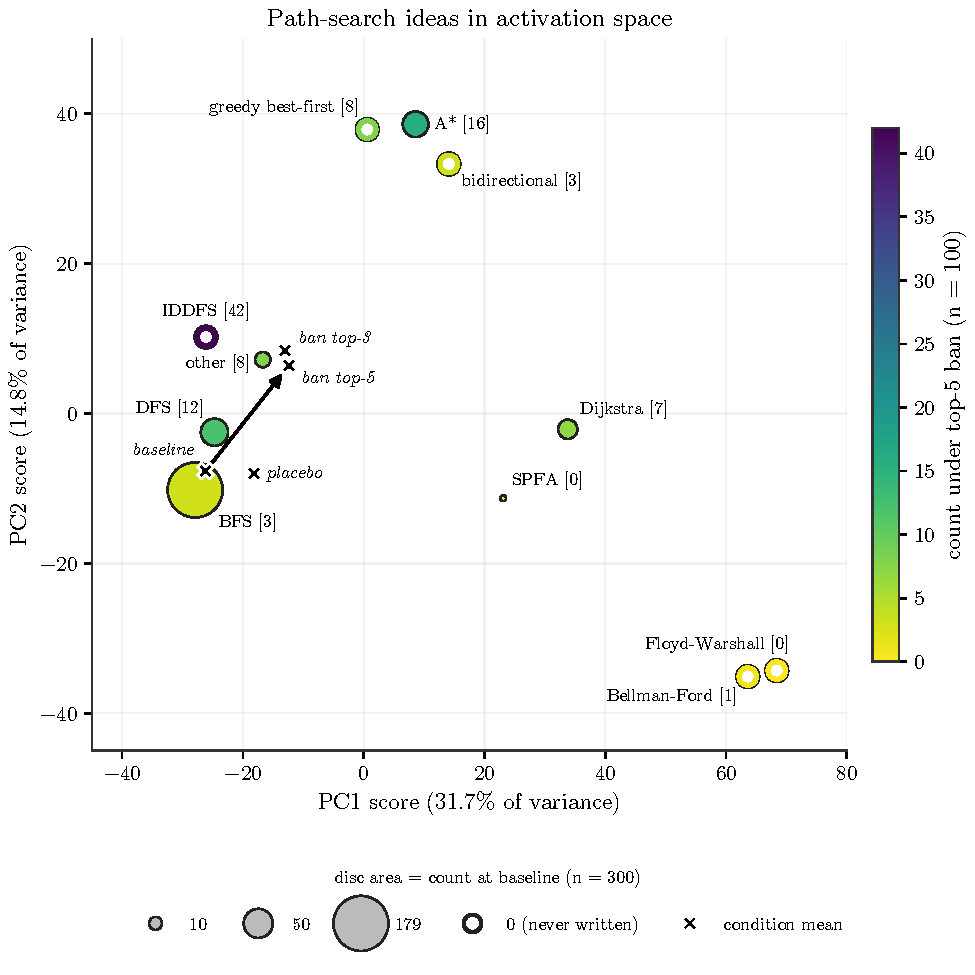
\includegraphics[width=\linewidth,height=0.85\textheight,keepaspectratio]{figures/fig_manifold_T1_v0.pdf}
\caption{Idea centroids of commitment-window activations (Qwen2.5-3B-Instruct, mean over layers 32 to 34, open path-search task) on the first two principal components, PC1 and PC2 (31.7\% and 14.8\% of variance). The PCA and the centroids are fitted on 700 programs: the 300 baseline programs plus 40 per idea from prompts that ask for that idea. Disc area is the idea's count among the 300 baseline programs (key below the plot). Ideas never written at baseline are drawn as white-centred rings. Colour is the idea's count among 100 programs under the top-5 ban (BFS, DFS, A*, Dijkstra and SPFA banned; colour bar 0 to 42). The same count appears in brackets after each name. Black crosses mark the mean point of the baseline, placebo, ban top-3 and ban top-5 programs, and the arrow runs from the baseline mean to the ban top-5 mean. Without the ban, most programs sit in the BFS/DFS basin on the left (BFS 179 of 300). Under the ban, the largest share goes to IDDFS [42], next to the banned BFS and DFS, and further mass goes to the heuristic cluster at the top: greedy best-first [8], bidirectional [3], and A* [16], which is written despite being banned. Almost none goes to the shortest-path family on the far right (Bellman-Ford [1], Floyd-Warshall [0]). Centroids are point means with no uncertainty shown; one model and one ban wording. [Source: artifact gen\_art\_experiment\_5, iteration 2.]}
\label{fig:fig_manifold_T1}
\end{figure}

\begingroup\small
\setlength{\tabcolsep}{4.0pt}
\begin{longtable}{@{}>{\raggedright\arraybackslash\hspace{0pt}}p{85.06pt}>{\raggedright\arraybackslash\hspace{0pt}}p{128.24pt}>{\raggedright\arraybackslash\hspace{0pt}}p{101.82pt}>{\raggedright\arraybackslash\hspace{0pt}}p{122.63pt}@{}}
\caption{Manifold summary per task (commitment-window activations, band layers). [Source: artifact gen\_art\_experiment\_5, iteration 2.]}\label{tab:64}\\
\toprule
\textbf{task} & \textbf{explained variance PC1 / PC2 / PC3} & \textbf{\ensuremath{\eta}\ensuremath{^2} of idea label on PC1 / PC2 / PC3} & \textbf{largest R\ensuremath{^2} of PC1 on a surface feature} \\
\midrule
\endfirsthead
\multicolumn{4}{@{}l}{\emph{(continued)}}\\
\toprule
\textbf{task} & \textbf{explained variance PC1 / PC2 / PC3} & \textbf{\ensuremath{\eta}\ensuremath{^2} of idea label on PC1 / PC2 / PC3} & \textbf{largest R\ensuremath{^2} of PC1 on a surface feature} \\
\midrule
\endhead
\bottomrule
\endlastfoot
open path search & 0.317 / 0.148 / 0.075 & 0.77 / 0.75 / 0.39 & 0.079 (n headers) \\
sorting & 0.237 / 0.144 / 0.087 & 0.82 / 0.69 / 0.56 & 0.118 (n headers) \\
weighted shortest path & 0.228 / 0.152 / 0.118 & 0.57 / 0.68 / 0.69 & 0.163 (prose before code) \\
k-th smallest & 0.440 / 0.125 / 0.067 & 0.28 / 0.08 / 0.70 & 0.106 (prose before code) \\
\end{longtable}
\endgroup
\begingroup\footnotesize
\setlength{\tabcolsep}{3.0pt}
\begin{longtable}{@{}>{\raggedright\arraybackslash\hspace{0pt}}p{92.67pt}>{\raggedright\arraybackslash\hspace{0pt}}p{108.55pt}>{\raggedright\arraybackslash\hspace{0pt}}p{42.14pt}>{\raggedright\arraybackslash\hspace{0pt}}p{40.90pt}>{\raggedright\arraybackslash\hspace{0pt}}p{41.85pt}>{\raggedright\arraybackslash\hspace{0pt}}p{49.41pt}>{\raggedright\arraybackslash\hspace{0pt}}p{52.23pt}@{}}
\caption{Idea centroids on the first three principal components, with baseline counts (n = 300) and the number of programs (baseline, ban and forced) behind each centroid. [Source: artifact gen\_art\_experiment\_5, iteration 2.]}\label{tab:65}\\
\toprule
\textbf{task} & \textbf{idea} & \textbf{PC1} & \textbf{PC2} & \textbf{PC3} & \textbf{baseline count (n=300)} & \textbf{programs used for the centroid} \\
\midrule
\endfirsthead
\multicolumn{7}{@{}l}{\emph{(continued)}}\\
\toprule
\textbf{task} & \textbf{idea} & \textbf{PC1} & \textbf{PC2} & \textbf{PC3} & \textbf{baseline count (n=300)} & \textbf{programs used for the centroid} \\
\midrule
\endhead
\bottomrule
\endlastfoot
open path search & BFS & -27.9 & -10.2 & 6.1 & 179 & 226 \\
open path search & A* & 8.6 & 38.6 & -11.8 & 39 & 98 \\
open path search & DFS & -24.7 & -2.5 & 12.6 & 44 & 83 \\
open path search & Dijkstra & 33.8 & -2.1 & 7.6 & 22 & 71 \\
open path search & Bellman-Ford & 63.6 & -35.1 & -3.0 & 0 & 40 \\
open path search & Floyd-Warshall & 68.4 & -34.3 & -8.7 & 0 & 40 \\
open path search & SPFA & 23.1 & -11.3 & -22.0 & 2 & 36 \\
open path search & IDDFS & -26.1 & 10.2 & -24.4 & 0 & 34 \\
open path search & other & -16.7 & 7.2 & 7.1 & 14 & 29 \\
open path search & bidirectional & 14.1 & 33.3 & 10.1 & 0 & 25 \\
open path search & greedy best-first & 0.6 & 37.9 & -10.4 & 0 & 18 \\
sorting & bubble sort & 34.6 & 19.1 & -3.7 & 179 & 219 \\
sorting & quicksort & 7.5 & -34.7 & 10.7 & 70 & 111 \\
sorting & merge sort & 0.3 & -29.7 & 12.4 & 31 & 73 \\
sorting & selection sort & 7.7 & 14.3 & 16.1 & 15 & 55 \\
sorting & insertion sort & 1.3 & 13.6 & 7.3 & 5 & 45 \\
sorting & bucket sort & -48.9 & 11.4 & -8.1 & 0 & 40 \\
sorting & counting sort & -38.6 & 6.5 & -35.5 & 0 & 40 \\
sorting & heap sort & -25.1 & -9.3 & 23.2 & 0 & 40 \\
sorting & radix sort & -54.5 & 13.6 & -27.9 & 0 & 40 \\
sorting & shell sort & -29.9 & 4.4 & -0.1 & 0 & 37 \\
sorting & Timsort/hybrid & -28.0 & -16.5 & -14.3 & 0 & 37 \\
sorting & other & -28.4 & -1.0 & -5.3 & 0 & 3 \\
weighted shortest path & Dijkstra & 1.0 & -12.5 & 8.2 & 300 & 361 \\
weighted shortest path & Bellman-Ford & 40.4 & 7.8 & -22.8 & 0 & 41 \\
weighted shortest path & A* & -27.8 & 47.3 & 27.0 & 0 & 40 \\
weighted shortest path & Floyd-Warshall & 44.6 & 18.3 & -34.7 & 0 & 37 \\
weighted shortest path & bidirectional & -24.9 & 32.7 & -7.8 & 0 & 34 \\
weighted shortest path & BFS & -31.0 & 4.5 & -27.1 & 0 & 33 \\
weighted shortest path & SPFA & -9.7 & 5.8 & -15.9 & 0 & 14 \\
weighted shortest path & IDDFS & -44.3 & 8.3 & -26.3 & 0 & 8 \\
weighted shortest path & DFS & -34.2 & 14.2 & -17.2 & 0 & 6 \\
weighted shortest path & other & 25.8 & 19.1 & -28.5 & 0 & 4 \\
weighted shortest path & greedy best-first & -44.2 & 33.3 & 0.6 & 0 & 2 \\
k-th smallest & quickselect & -17.2 & -5.7 & 0.2 & 226 & 312 \\
k-th smallest & sort then index & 5.3 & 8.0 & -1.3 & 59 & 113 \\
k-th smallest & heap select & 38.4 & 7.0 & -34.4 & 14 & 57 \\
k-th smallest & median of medians & -2.3 & 0.8 & 30.3 & 1 & 42 \\
k-th smallest & counting/bucket & 50.2 & 4.4 & 14.8 & 0 & 39 \\
k-th smallest & binary search on value & 46.8 & 18.1 & 11.9 & 0 & 11 \\
k-th smallest & partial selection & 36.6 & 14.3 & 8.1 & 0 & 6 \\
\end{longtable}
\endgroup
\begingroup\footnotesize
\setlength{\tabcolsep}{3.0pt}
\begin{longtable}{@{}>{\raggedright\arraybackslash\hspace{0pt}}p{68.68pt}>{\raggedright\arraybackslash\hspace{0pt}}p{68.06pt}>{\raggedright\arraybackslash\hspace{0pt}}p{52.83pt}>{\raggedright\arraybackslash\hspace{0pt}}p{72.63pt}>{\raggedright\arraybackslash\hspace{0pt}}p{177.54pt}@{}}
\caption{Mean point of each screen condition on PC1 and PC2, the norm of its prompt displacement against the placebo, and its idea counts. [Source: artifact gen\_art\_experiment\_5, iteration 2.]}\label{tab:66}\\
\toprule
\textbf{task} & \textbf{condition} & \textbf{mean point PC1, PC2} & \textbf{prompt displacement norm (suffix)} & \textbf{idea counts} \\
\midrule
\endfirsthead
\multicolumn{5}{@{}l}{\emph{(continued)}}\\
\toprule
\textbf{task} & \textbf{condition} & \textbf{mean point PC1, PC2} & \textbf{prompt displacement norm (suffix)} & \textbf{idea counts} \\
\midrule
\endhead
\bottomrule
\endlastfoot
open path search & baseline (n=300) & -26.2, -7.7 & 16.04 & BFS 179, DFS 44, A* 39, Dijkstra 22, other 14, SPFA 2 \\
open path search & placebo & -18.2, -8.0 & 0.00 & BFS 67, DFS 17, Dijkstra 11, other 4, A* 1 \\
open path search & ban rank-1 & -16.4, 3.3 & 8.98 & DFS 66, other 15, A* 11, Dijkstra 7, BFS 1 \\
open path search & ban rank-2 & -28.7, -8.8 & 8.37 & BFS 98, A* 2 \\
open path search & ban rank-3 & -23.7, -1.9 & 8.93 & BFS 69, DFS 17, Dijkstra 8, SPFA 4, other 2 \\
open path search & ban rank-4 & -11.1, 10.4 & 10.29 & BFS 44, A* 34, DFS 16, other 3, SPFA 2, Dijkstra 1 \\
open path search & ban top-3 & -13.0, 8.4 & 15.86 & IDDFS 42, DFS 18, Dijkstra 16, A* 8, other 6, bidirectional 4, BFS 3, greedy best-first 2, Bellman-Ford 1 \\
open path search & ban top-5 & -12.4, 6.4 & 19.81 & IDDFS 42, A* 16, DFS 12, greedy best-first 8, other 8, Dijkstra 7, BFS 3, bidirectional 3, Bellman-Ford 1 \\
open path search & ban rare idea & 0.4, -8.4 & 8.94 & Dijkstra 50, BFS 42, A* 6, Bellman-Ford 1, DFS 1 \\
sorting & baseline (n=300) & 28.9, -2.5 & 23.42 & bubble sort 179, quicksort 70, merge sort 31, selection sort 15, insertion sort 5 \\
sorting & placebo & 29.4, -11.3 & 0.00 & bubble sort 43, merge sort 26, quicksort 18, selection sort 8, insertion sort 5 \\
sorting & ban rank-1 & 20.6, -34.1 & 10.84 & quicksort 71, merge sort 27, heap sort 1, insertion sort 1 \\
sorting & ban rank-2 & 20.4, -11.5 & 11.25 & insertion sort 41, merge sort 30, bubble sort 15, selection sort 13, heap sort 1 \\
sorting & ban rank-3 & 30.9, -11.1 & 9.70 & bubble sort 45, quicksort 23, insertion sort 14, selection sort 14, heap sort 4 \\
sorting & ban rank-4 & 26.2, -17.1 & 11.78 & bubble sort 41, merge sort 39, quicksort 10, insertion sort 9, heap sort 1 \\
sorting & ban top-3 & 15.9, -8.7 & 13.48 & selection sort 55, insertion sort 42, counting sort 2, heap sort 1 \\
sorting & ban top-5 & 3.0, -11.1 & 17.93 & counting sort 45, heap sort 26, shell sort 7, bubble sort 6, other 6, bucket sort 5, radix sort 4, merge sort 1 \\
sorting & ban rare idea & 15.5, -33.7 & 11.02 & quicksort 66, merge sort 27, heap sort 4, selection sort 2, bubble sort 1 \\
weighted shortest path & baseline (n=300) & -0.8, -17.6 & 15.58 & Dijkstra 300 \\
weighted shortest path & placebo & -3.4, -17.2 & 0.00 & Dijkstra 100 \\
weighted shortest path & ban rank-1 & -28.2, -13.6 & 19.19 & Bellman-Ford 55, BFS 19, Dijkstra 12, A* 8, bidirectional 2, Floyd-Warshall 1, greedy best-first 1, other 1, SPFA 1 \\
weighted shortest path & ban rank-2 & -25.9, -12.5 & 8.84 & Dijkstra 95, BFS 4, SPFA 1 \\
weighted shortest path & ban rank-3 & -13.0, -19.5 & 9.28 & Dijkstra 100 \\
weighted shortest path & ban rank-4 & -7.4, -18.0 & 6.74 & Dijkstra 100 \\
weighted shortest path & ban top-3 & -30.5, -13.3 & 21.33 & BFS 32, Dijkstra 25, Bellman-Ford 21, SPFA 7, Floyd-Warshall 5, DFS 3, other 3, bidirectional 1, greedy best-first 1, IDDFS 1, unparseable 1 \\
weighted shortest path & ban top-5 & -24.1, -10.3 & 20.01 & Dijkstra 41, BFS 26, Bellman-Ford 16, SPFA 10, bidirectional 2, A* 1, DFS 1, Floyd-Warshall 1, greedy best-first 1, other 1 \\
weighted shortest path & ban rare idea & -8.0, -8.2 & 8.30 & Dijkstra 98, BFS 1, DFS 1 \\
\end{longtable}
\endgroup
The centroid geometry is stable within a run (split-half median similarity 0.973, 0.981 and 0.954 on path search, sorting and the weighted task) but agrees only partly between natural and forced programs of the same idea (Spearman 0.36 over 5 ideas on path search and 0.83 over 4 on sorting; the weighted task has too few natural ideas to compare). Centroids from forced programs are a noisy stand-in for how the model represents an idea it chose on its own.

\subsection{Steering on the bare prompt: selection confirmed, flattening not seen, and a second model}
\subsubsection{Iteration 1's random-control claim, re-analysed}
The third artifact first re-analysed the influence arm's random-control comparison as the review required (\texttt{gen\_\allowbreak{}art\_\allowbreak{}experiment\_\allowbreak{}6}). Each of the 18 targeted settings (three strengths per knob family on each of the two tasks, the strengths at which random draws exist) was compared with the mean entropy of the three random draws at the same strength. The comparison used Miller-Madow-corrected entropy on n-matched seeds 0 to 74 and a hierarchical bootstrap that resamples draws, then samples within draws. Three settings beat the draw mean, five are significantly below it and ten are undetermined (Tables 67 and 68). The below-mean settings are four difference-in-means and probe-weight settings on the open task, which select DFS, and the probe-weight direction at \ensuremath{\alpha} = 1.5 on the weighted task; the settings above the mean are the novelty direction at \ensuremath{\alpha} = 0.632 on the open task and the difference-in-means direction at \ensuremath{\alpha} = 0.224 and 0.473 on the weighted task. With only three random draws at n = 75, draw-level variance is poorly estimated, so most comparisons cannot be resolved. The statement that random directions raise idea entropy as much as targeted ones is withdrawn. The defensible statement is that, where targeted directions select, they lower entropy below random, and elsewhere the data cannot separate them.

\begingroup\footnotesize
\setlength{\tabcolsep}{3.0pt}
\begin{longtable}{@{}>{\raggedright\arraybackslash\hspace{0pt}}p{47.36pt}>{\raggedright\arraybackslash\hspace{0pt}}p{104.99pt}>{\raggedright\arraybackslash\hspace{0pt}}p{44.26pt}>{\raggedright\arraybackslash\hspace{0pt}}p{43.65pt}>{\raggedright\arraybackslash\hspace{0pt}}p{62.27pt}>{\raggedright\arraybackslash\hspace{0pt}}p{60.38pt}>{\raggedright\arraybackslash\hspace{0pt}}p{64.84pt}@{}}
\caption{Iteration-1 targeted settings against the draw-averaged random entropy (primary specification: Miller-Madow, n-matched seeds 0..74). [Source: artifact gen\_art\_experiment\_6, iteration 2.]}\label{tab:67}\\
\toprule
\textbf{task} & \textbf{setting} & \textbf{targeted entropy (bits, Miller-Madow, n=75)} & \textbf{random draw mean (draws 0, 1, 2)} & \textbf{difference [95\% CI]} & \textbf{verdict} & \textbf{iteration-1 comparison (pooled draws): difference, verdict} \\
\midrule
\endfirsthead
\multicolumn{7}{@{}l}{\emph{(continued)}}\\
\toprule
\textbf{task} & \textbf{setting} & \textbf{targeted entropy (bits, Miller-Madow, n=75)} & \textbf{random draw mean (draws 0, 1, 2)} & \textbf{difference [95\% CI]} & \textbf{verdict} & \textbf{iteration-1 comparison (pooled draws): difference, verdict} \\
\midrule
\endhead
\bottomrule
\endlastfoot
open path search & probe-weight direction, alpha = 1.06 & 0.760 & 1.177 (1.11, 1.10, 1.31) & -0.417 [-0.815, -0.063] & below & -0.498, below \\
open path search & probe-weight direction, alpha = 1.26 & 1.060 & 1.229 (0.79, 1.26, 1.64) & -0.169 [-0.715, +0.233] & undetermined & -0.463, below \\
open path search & probe-weight direction, alpha = 1.5 & 1.060 & 1.297 (0.73, 1.26, 1.90) & -0.237 [-0.877, +0.306] & undetermined & -0.634, below \\
open path search & difference-in-means direction, alpha = 0.224 & 0.223 & 1.113 (0.99, 1.21, 1.14) & -0.890 [-1.162, -0.623] & below & -0.892, below \\
open path search & difference-in-means direction, alpha = 0.473 & 0.659 & 1.135 (1.04, 1.36, 1.01) & -0.477 [-0.829, -0.141] & below & -0.713, below \\
open path search & difference-in-means direction, alpha = 1 & 0.000 & 1.222 (1.12, 1.23, 1.31) & -1.222 [-2.037, -1.025] & below & -0.287, below \\
open path search & novelty direction, alpha = 0.632 & 1.889 & 1.215 (1.12, 1.52, 1.00) & +0.674 [+0.262, +1.000] & beats & +0.496, beats \\
open path search & novelty direction, alpha = 1.12 & 1.427 & 1.299 (1.19, 1.17, 1.54) & +0.128 [-0.203, +0.450] & undetermined & +0.092, undetermined \\
open path search & novelty direction, alpha = 2 & 1.285 & 1.568 (1.56, 1.47, 1.67) & -0.283 [-0.529, +0.110] & undetermined & -0.219, undetermined \\
weighted shortest path & probe-weight direction, alpha = 1.06 & 1.495 & 1.146 (1.26, 0.90, 1.28) & +0.348 [-0.001, +0.705] & undetermined & +0.278, beats \\
weighted shortest path & probe-weight direction, alpha = 1.26 & 1.203 & 1.436 (1.69, 1.15, 1.47) & -0.234 [-0.649, +0.228] & undetermined & -0.201, undetermined \\
weighted shortest path & probe-weight direction, alpha = 1.5 & 0.919 & 1.428 (1.29, 1.38, 1.61) & -0.510 [-0.984, -0.067] & below & -0.763, below \\
weighted shortest path & difference-in-means direction, alpha = 0.224 & 1.446 & 1.033 (1.11, 0.85, 1.15) & +0.413 [+0.057, +0.709] & beats & +0.374, beats \\
weighted shortest path & difference-in-means direction, alpha = 0.473 & 1.530 & 1.111 (1.00, 1.04, 1.29) & +0.419 [+0.023, +0.715] & beats & +0.302, beats \\
weighted shortest path & difference-in-means direction, alpha = 1 & 1.453 & 1.105 (1.01, 0.78, 1.53) & +0.349 [-0.486, +0.841] & undetermined & -0.210, undetermined \\
weighted shortest path & novelty direction, alpha = 0.632 & 1.298 & 1.008 (0.96, 0.95, 1.12) & +0.290 [-0.106, +0.652] & undetermined & +0.118, undetermined \\
weighted shortest path & novelty direction, alpha = 1.12 & 1.123 & 1.220 (1.58, 0.72, 1.36) & -0.097 [-0.626, +0.461] & undetermined & -0.454, below \\
weighted shortest path & novelty direction, alpha = 2 & 0.672 & 1.042 (0.95, 1.02, 1.16) & -0.370 [-0.713, +0.078] & undetermined & -0.456, below \\
\end{longtable}
\endgroup
\begingroup\footnotesize
\setlength{\tabcolsep}{3.0pt}
\begin{longtable}{@{}>{\raggedright\arraybackslash\hspace{0pt}}p{253.25pt}>{\raggedright\arraybackslash\hspace{0pt}}p{43.18pt}>{\raggedright\arraybackslash\hspace{0pt}}p{43.18pt}>{\raggedright\arraybackslash\hspace{0pt}}p{75.80pt}>{\raggedright\arraybackslash\hspace{0pt}}p{24.34pt}@{}}
\caption{How the verdict depends on the specification (counts out of 18 targeted settings). [Source: artifact gen\_art\_experiment\_6, iteration 2.]}\label{tab:68}\\
\toprule
\textbf{specification} & \textbf{beats draw mean} & \textbf{below draw mean} & \textbf{undetermined} & \textbf{n} \\
\midrule
\endfirsthead
\multicolumn{5}{@{}l}{\emph{(continued)}}\\
\toprule
\textbf{specification} & \textbf{beats draw mean} & \textbf{below draw mean} & \textbf{undetermined} & \textbf{n} \\
\midrule
\endhead
\bottomrule
\endlastfoot
Miller-Madow, n-matched seeds 0..74 (primary) & 3 & 5 & 10 & 18 \\
Miller-Madow, targeted n=150 & 5 & 5 & 8 & 18 \\
plug-in, targeted n=150 & 5 & 6 & 7 & 18 \\
plug-in, n-matched & 4 & 5 & 9 & 18 \\
plug-in, pooled draws (iteration-1 comparison) & 4 & 9 & 5 & 18 \\
plug-in, single draw 0 (iteration-1 survival rule) & 7 & 4 & 7 & 18 \\
rule-classifier relabel, Miller-Madow n-matched & 4 & 7 & 7 & 18 \\
rule-classifier relabel, plug-in n=150 & 6 & 5 & 7 & 18 \\
\end{longtable}
\endgroup
The novelty-direction dose-response is not significant by exact permutation (Table 69).

\begingroup\footnotesize
\setlength{\tabcolsep}{3.0pt}
\begin{longtable}{@{}>{\raggedright\arraybackslash\hspace{0pt}}p{66.19pt}>{\raggedright\arraybackslash\hspace{0pt}}p{56.86pt}>{\raggedright\arraybackslash\hspace{0pt}}p{95.86pt}>{\raggedright\arraybackslash\hspace{0pt}}p{72.46pt}>{\raggedright\arraybackslash\hspace{0pt}}p{68.45pt}>{\raggedright\arraybackslash\hspace{0pt}}p{73.93pt}@{}}
\caption{Exact permutation test of the novelty direction's Spearman correlation between strength and atypicality (6 strength points). [Source: artifact gen\_art\_experiment\_6, iteration 2.]}\label{tab:69}\\
\toprule
\textbf{task} & \textbf{Spearman rho} & \textbf{exact two-sided p (720 permutations)} & \textbf{one-sided p (positive)} & \textbf{original CI} & \textbf{corrected CI} \\
\midrule
\endfirsthead
\multicolumn{6}{@{}l}{\emph{(continued)}}\\
\toprule
\textbf{task} & \textbf{Spearman rho} & \textbf{exact two-sided p (720 permutations)} & \textbf{one-sided p (positive)} & \textbf{original CI} & \textbf{corrected CI} \\
\midrule
\endhead
\bottomrule
\endlastfoot
open path search & 0.486 & 0.356 & 0.178 & [-0.029, 0.543] & [-0.429, 0.600] \\
weighted shortest path & -0.257 & 0.658 & 0.718 & [-0.486, 0.143] & [-1.000, 0.086] \\
\end{longtable}
\endgroup
\textbf{How this compares with published steering results.} The selector finding agrees with the reliability literature. Tan et al. [13] find that steerability varies widely across inputs and that steering vectors can fail on some concepts. Turner et al. [7] report that a matched-norm random vector barely changes outputs. Our iteration-1 random draws did change the idea mix, by up to 0.65 bits of pooled entropy in a single draw (Table 15), but the draw-averaged re-analysis no longer supports parity. Olson et al. [14] extract a direction from "boring" against "creative" prompts and report that adding it raises the creativity of text. That is close to our cross-task novelty direction, which transferred perfectly as a readout (AUROC 1.0) but did not raise atypicality monotonically in code (Table 69). STARS [15] and Riemannian activation steering [16] report diversity gains over plain sampling. They do so by optimising several steering directions jointly across concurrent generations at test time, which is a different intervention from one fixed direction. What this run adds to these comparisons is execution-verified correctness, algorithm-level labels in place of lexical diversity, five matched-norm random draws per strength, and a fresh-seed re-draw. Candidate reasons for the disagreement with the creativity-steering results are the task (code with a small menu of textbook ideas, not open text), the model size (3B), the late layers (29 to 34 of 36), and the window of the first 64 generated tokens.

\subsubsection{Select or flatten: the pre-registered test on the bare prompt}
\textbf{Design.} On the bare prompt, with menus of four or more ideas, a direction that flattens and a direction that selects make different predictions. A flattener lowers the mode share without making any single other idea dominant, so the distance from uniform falls steadily with strength. A selector hands most of the mass to one other idea. The artifact built the \emph{away-from-mode direction} as the difference in means of commitment-window activations at layers 32 to 34 between non-modal and modal programs, unit-normalised per layer. It added the direction at the prompt-final token and the first 64 generated tokens with strength \ensuremath{\alpha} times the layer's median residual norm divided by three, as in iteration 1. Comparators were five matched-norm random directions per strength, an off-target real direction (the other task's away-from-mode direction), temperature 1.0 and 1.3, directions toward the centroids of two off-menu ideas (IDDFS and Bellman-Ford on path search, counting and heap sort on sorting), and simply asking for those ideas. The frozen rules (sha256 files) were:

\begin{itemize}
\item strength s1: the \ensuremath{\alpha} whose mode share is closest to half the baseline mode share;
\item strength s2: the \ensuremath{\alpha} with the lowest mode share whose pass rate stays at least 0.8 times the baseline's (calibrated on n = 30);
\item SELECT: at s2 one non-modal idea takes at least half the samples, that idea was a predicted gainer, and the distance from uniform rises again from s1 to s2;
\item FLATTEN: the distance from uniform falls from baseline to s1 to s2 and no non-modal idea reaches half the samples.
\end{itemize}
Predicted gainers came from two frozen rankings. One is the projection of the away-from-mode direction onto each centroid's offset from the mode; the other is each centroid's nearest-neighbour similarity to the modal centroid. For path search, the projection ranking is A*, Dijkstra, other, DFS, Bellman-Ford, IDDFS (scores A* 0.843, Dijkstra 0.742, other 0.685, DFS 0.656, Bellman-Ford 0.401, IDDFS 0.363); the nearest-neighbour ranking is IDDFS, Bellman-Ford, DFS, other, Dijkstra, A*. For sorting, the projection ranking is quicksort, merge sort, heap sort, selection sort, insertion sort, counting sort (scores quicksort 0.973, merge sort 0.887, heap sort 0.521, selection sort 0.488, insertion sort 0.480, counting sort 0.429); the nearest-neighbour ranking is selection sort, insertion sort, counting sort, heap sort, merge sort, quicksort. Main runs used seeds 0 to 149 and a re-draw used seeds 1000 to 1149, both on the HF engine.

\textbf{Result: SELECT on both tasks, replicated on both draws.} On path search at s2 (\ensuremath{\alpha} = 0.224), BFS falls from 61\% to 13\% and A* rises to 57\% (main) and 63\% (re-draw). A* was the projection ranking's top predicted gainer. None of the five random draws makes A* the top gainer, and they leave BFS at 61\% to 72\%. The non-mode share is 0.54 above the random-draw mean [0.47, 0.61]. The cost is correctness: the pass rate falls to 0.17 against 0.34 for the random-draw mean, below the 0.8 bar the n = 30 calibration had predicted, and 78\% of outputs hit the token cap. On sorting at s2 (\ensuremath{\alpha} = 0.473), bubble sort falls from 62\% to 1\% and 0\%, and quicksort rises to 65\% and 68\%, again the projection ranking's prediction, at a pass rate of 0.92. Sorting entropy at s2 is 0.71 bits below the random-draw mean [\ensuremath{-}0.94, \ensuremath{-}0.44], the signature of selection. On path search entropy at s2 is above the random mean on the main draw (+0.32 [0.04, 0.56]) and undetermined on the re-draw (+0.10 [\ensuremath{-}0.19, 0.36]), because the path-search baseline mode is so dominant that moving mass to A* while BFS, DFS and Dijkstra keep 11\% to 15\% each raises entropy even though one idea takes over. The nearest-neighbour ranking (IDDFS on path search, selection sort on sorting) was wrong on both tasks. The direction lands on the idea along its own projection, not on the idea that sits closest to the mode.

Tables 70 to 73 give every cell and every comparison with the random-draw mean. Some random draws also move sorting a lot: draw 3 at s2 gives selection sort 72 of 150, and draw 0 gives quicksort 75. The random-draw mode share at s2 ranges from 0.19 to 0.69. A single random cell would have misled either way, which is why the comparison is against the mean of five draws.

\begin{figure}[!htbp]
\centering
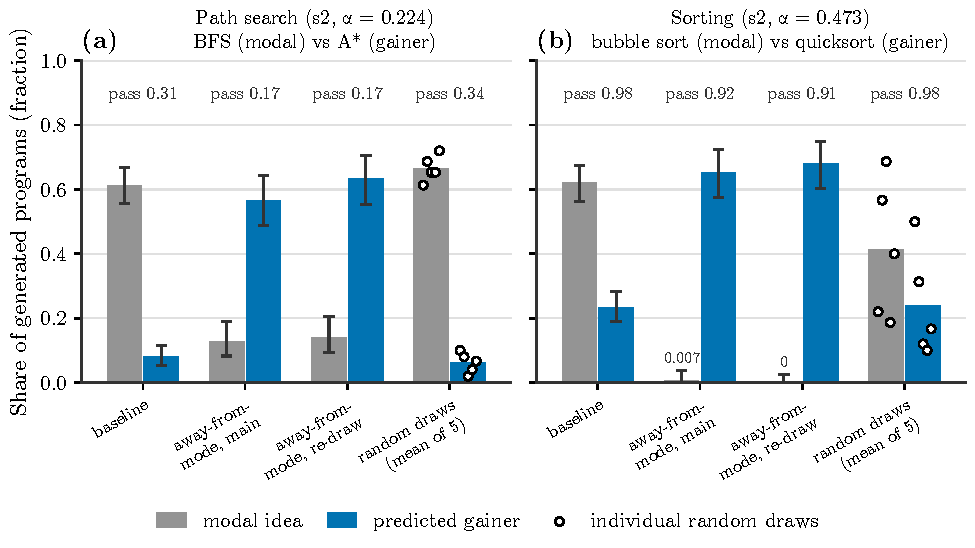
\includegraphics[width=\linewidth,height=0.85\textheight,keepaspectratio]{figures/fig_selector_v0.pdf}
\caption{Pre-registered select-or-flatten test on the bare prompt (Qwen2.5-3B-Instruct, HF engine). The y-axis is the share of generated programs labelled as each idea. Grey bars are the modal idea and blue bars the frozen predicted gainer: (a) path search, BFS and A$^*$ at strength s2 ($\alpha = 0.224$); (b) sorting, bubble sort and quicksort at s2 ($\alpha = 0.473$). Groups show the baseline ($n = 300$), the away-from-mode direction on the main draw and on the fresh-seed re-draw ($n = 150$ each), and the mean over five matched-norm random directions at the same strength ($n = 150$ each). Open circles are the five individual random draws. Error bars are Wilson 95\% confidence intervals on each share; none are drawn on the random-draw mean, whose spread the circles show. Bubble-sort shares under steering (1/150 and 0/150) are printed because the bars are too short to see. The oracle pass rate of each group is printed above it. The targeted direction moves most of the mass from the modal idea to the predicted gainer on both tasks and both draws (A$^*$ 0.08 $\rightarrow$ 0.57/0.63; quicksort 0.23 $\rightarrow$ 0.65/0.68). On path search this comes with a lower pass rate (0.31 $\rightarrow$ 0.17). Random directions leave the modal idea dominant on average, although individual sorting draws vary widely (one raises quicksort to 0.50). [Source: artifact gen\_art\_experiment\_6, iteration 2.]}
\label{fig:fig_selector}
\end{figure}

\begingroup\scriptsize
\setlength{\tabcolsep}{2.0pt}
\begin{longtable}{@{}>{\raggedright\arraybackslash\hspace{0pt}}p{109.09pt}>{\raggedright\arraybackslash\hspace{0pt}}p{18.79pt}>{\raggedright\arraybackslash\hspace{0pt}}p{125.30pt}>{\raggedright\arraybackslash\hspace{0pt}}p{42.29pt}>{\raggedright\arraybackslash\hspace{0pt}}p{31.26pt}>{\raggedright\arraybackslash\hspace{0pt}}p{26.87pt}>{\raggedright\arraybackslash\hspace{0pt}}p{48.47pt}>{\raggedright\arraybackslash\hspace{0pt}}p{35.67pt}@{}}
\caption{Selector test, open path search (Qwen, HF engine, bare prompt). The last five rows are the n = 30 strength calibration. [Source: artifact gen\_art\_experiment\_6, iteration 2.]}\label{tab:70}\\
\toprule
\textbf{setting} & \textbf{n} & \textbf{idea counts} & \textbf{idea entropy (bits)} & \textbf{mode share} & \textbf{pass rate} & \textbf{truncated} & \textbf{off-menu correct} \\
\midrule
\endfirsthead
\multicolumn{8}{@{}l}{\emph{(continued)}}\\
\toprule
\textbf{setting} & \textbf{n} & \textbf{idea counts} & \textbf{idea entropy (bits)} & \textbf{mode share} & \textbf{pass rate} & \textbf{truncated} & \textbf{off-menu correct} \\
\midrule
\endhead
\bottomrule
\endlastfoot
baseline (seeds 0..299) & 300 & BFS 184, DFS 42, Dijkstra 36, A* 24, other 11, SPFA 3 & 1.730 & 0.61 & 0.31 & 0.42 & 0 \\
away-from-mode direction, s1 & 150 & BFS 78, A* 27, Dijkstra 24, DFS 11, other 8, SPFA 2 & 1.944 & 0.52 & 0.35 & 0.46 & 1 \\
away-from-mode direction, s2 & 150 & A* 85, DFS 22, BFS 19, Dijkstra 17, other 5, SPFA 1, greedy best-first 1 & 1.864 & 0.13 & 0.17 & 0.78 & 0 \\
away-from-mode, s1, re-draw & 150 & BFS 85, A* 26, DFS 18, Dijkstra 14, other 5, bidirectional 1, SPFA 1 & 1.849 & 0.57 & 0.33 & 0.44 & 1 \\
away-from-mode, s2, re-draw & 150 & A* 95, BFS 21, DFS 19, Dijkstra 11, other 2, SPFA 1, greedy best-first 1 & 1.648 & 0.14 & 0.17 & 0.77 & 0 \\
off-target real direction (other task), s2 & 150 & BFS 56, A* 40, DFS 32, Dijkstra 12, other 8, SPFA 1, bidirectional 1 & 2.128 & 0.37 & 0.21 & 0.52 & 0 \\
temperature 1.0 & 150 & BFS 91, DFS 28, Dijkstra 14, A* 8, other 8, SPFA 1 & 1.708 & 0.61 & 0.23 & 0.49 & 1 \\
temperature 1.3 & 150 & BFS 63, other 36, DFS 24, Dijkstra 16, A* 5, SPFA 3, greedy best-first 1 & 2.121 & 0.42 & 0.05 & 0.81 & 0 \\
random direction draw 0, s1 & 100 & BFS 59, DFS 20, Dijkstra 13, A* 8 & 1.588 & 0.59 & 0.29 & 0.42 & 0 \\
random direction draw 0, s2 & 150 & BFS 92, Dijkstra 21, A* 15, DFS 15, other 6, SPFA 1 & 1.728 & 0.61 & 0.28 & 0.41 & 0 \\
random direction draw 1, s1 & 100 & BFS 63, A* 13, DFS 13, Dijkstra 7, SPFA 2, other 2 & 1.680 & 0.63 & 0.26 & 0.45 & 1 \\
random direction draw 1, s2 & 150 & BFS 103, DFS 22, A* 12, Dijkstra 7, other 6 & 1.462 & 0.69 & 0.31 & 0.33 & 0 \\
random direction draw 2, s1 & 100 & BFS 70, DFS 13, Dijkstra 9, A* 8 & 1.347 & 0.70 & 0.32 & 0.38 & 0 \\
random direction draw 2, s2 & 150 & BFS 98, Dijkstra 21, DFS 20, other 5, A* 3, SPFA 3 & 1.575 & 0.65 & 0.41 & 0.37 & 2 \\
random direction draw 3, s1 & 100 & BFS 64, A* 13, DFS 13, Dijkstra 8, other 2 & 1.582 & 0.64 & 0.20 & 0.46 & 0 \\
random direction draw 3, s2 & 150 & BFS 98, DFS 21, Dijkstra 19, A* 6, other 5, greedy best-first 1 & 1.573 & 0.65 & 0.35 & 0.39 & 0 \\
random direction draw 4, s1 & 100 & BFS 71, Dijkstra 11, A* 10, DFS 8 & 1.325 & 0.71 & 0.30 & 0.45 & 0 \\
random direction draw 4, s2 & 150 & BFS 108, Dijkstra 17, A* 10, DFS 9, SPFA 3, other 3 & 1.427 & 0.72 & 0.34 & 0.48 & 1 \\
toward IDDFS centroid, s2 & 150 & DFS 53, BFS 49, A* 24, Dijkstra 13, other 11 & 2.063 & 0.33 & 0.30 & 0.43 & 0 \\
toward Bellman-Ford centroid, s2 & 150 & BFS 87, Dijkstra 52, A* 8, DFS 2, other 1 & 1.342 & 0.58 & 0.55 & 0.46 & 0 \\
prompt: "... using IDDFS." & 60 & IDDFS 55, BFS 4, other 1 & 0.474 & 0.07 & 0.03 & 0.32 & 2 \\
prompt: "... using Bellman-Ford." & 60 & Bellman-Ford 60 & -0.000 & 0.00 & 0.75 & 0.60 & 45 \\
baseline, seeds 0..149 & 150 & BFS 89, DFS 27, Dijkstra 18, A* 11, other 4, SPFA 1 & 1.723 & 0.59 & 0.26 & 0.42 & 0 \\
calibration, away-from-mode alpha = 0.05 & 30 & BFS 13, A* 7, Dijkstra 6, DFS 4 & 1.865 & 0.43 & 0.27 & 0.60 & 0 \\
calibration, away-from-mode alpha = 0.106 & 30 & BFS 14, Dijkstra 6, A* 5, DFS 3, other 2 & 2.001 & 0.47 & 0.33 & 0.37 & 0 \\
calibration, away-from-mode alpha = 0.224 & 30 & A* 14, Dijkstra 8, BFS 4, DFS 4 & 1.797 & 0.13 & 0.33 & 0.77 & 0 \\
calibration, away-from-mode alpha = 0.473 & 30 & A* 27, Dijkstra 2, DFS 1 & 0.561 & 0.00 & 0.07 & 0.90 & 0 \\
calibration, away-from-mode alpha = 1 & 30 & A* 21, Dijkstra 4, BFS 2 & 0.968 & 0.07 & 0.10 & 0.93 & 0 \\
\end{longtable}
\endgroup
\begingroup\scriptsize
\setlength{\tabcolsep}{2.0pt}
\begin{longtable}{@{}>{\raggedright\arraybackslash\hspace{0pt}}p{100.70pt}>{\raggedright\arraybackslash\hspace{0pt}}p{17.73pt}>{\raggedright\arraybackslash\hspace{0pt}}p{142.24pt}>{\raggedright\arraybackslash\hspace{0pt}}p{40.36pt}>{\raggedright\arraybackslash\hspace{0pt}}p{29.67pt}>{\raggedright\arraybackslash\hspace{0pt}}p{25.30pt}>{\raggedright\arraybackslash\hspace{0pt}}p{46.90pt}>{\raggedright\arraybackslash\hspace{0pt}}p{34.86pt}@{}}
\caption{Selector test, sorting. [Source: artifact gen\_art\_experiment\_6, iteration 2.]}\label{tab:71}\\
\toprule
\textbf{setting} & \textbf{n} & \textbf{idea counts} & \textbf{idea entropy (bits)} & \textbf{mode share} & \textbf{pass rate} & \textbf{truncated} & \textbf{off-menu correct} \\
\midrule
\endfirsthead
\multicolumn{8}{@{}l}{\emph{(continued)}}\\
\toprule
\textbf{setting} & \textbf{n} & \textbf{idea counts} & \textbf{idea entropy (bits)} & \textbf{mode share} & \textbf{pass rate} & \textbf{truncated} & \textbf{off-menu correct} \\
\midrule
\endhead
\bottomrule
\endlastfoot
baseline (seeds 0..299) & 300 & bubble sort 186, quicksort 70, merge sort 27, selection sort 11, insertion sort 5 & 1.504 & 0.62 & 0.98 & 0.07 & 5 \\
away-from-mode direction, s1 & 150 & quicksort 76, bubble sort 43, merge sort 21, selection sort 9, insertion sort 1 & 1.703 & 0.29 & 0.99 & 0.05 & 1 \\
away-from-mode direction, s2 & 150 & quicksort 98, merge sort 50, selection sort 1, bubble sort 1 & 1.026 & 0.01 & 0.92 & 0.06 & 0 \\
away-from-mode, s1, re-draw & 150 & quicksort 65, bubble sort 47, merge sort 28, insertion sort 6, selection sort 4 & 1.825 & 0.31 & 0.99 & 0.02 & 6 \\
away-from-mode, s2, re-draw & 150 & quicksort 102, merge sort 45, selection sort 3 & 1.012 & 0.00 & 0.91 & 0.08 & 0 \\
off-target real direction (other task), s2 & 150 & quicksort 52, merge sort 50, bubble sort 35, selection sort 11, other 1 & 1.876 & 0.23 & 0.98 & 0.07 & 0 \\
temperature 1.0 & 150 & bubble sort 65, quicksort 47, selection sort 17, merge sort 16, insertion sort 4, Timsort/hybrid 1 & 1.935 & 0.43 & 1.00 & 0.07 & 5 \\
temperature 1.3 & 150 & bubble sort 71, quicksort 38, merge sort 15, selection sort 15, insertion sort 5, other 5 & 2.008 & 0.47 & 0.81 & 0.32 & 5 \\
random direction draw 0, s1 & 100 & bubble sort 54, quicksort 28, merge sort 8, insertion sort 5, selection sort 5 & 1.718 & 0.54 & 0.98 & 0.09 & 5 \\
random direction draw 0, s2 & 150 & quicksort 75, bubble sort 33, merge sort 21, selection sort 18, insertion sort 2, Timsort/hybrid 1 & 1.876 & 0.22 & 0.97 & 0.09 & 2 \\
random direction draw 1, s1 & 100 & bubble sort 57, quicksort 26, merge sort 8, selection sort 6, insertion sort 3 & 1.654 & 0.57 & 0.98 & 0.07 & 3 \\
random direction draw 1, s2 & 150 & bubble sort 85, quicksort 47, merge sort 8, insertion sort 6, selection sort 4 & 1.540 & 0.57 & 0.99 & 0.05 & 6 \\
random direction draw 2, s1 & 100 & bubble sort 61, quicksort 25, merge sort 10, selection sort 2, insertion sort 2 & 1.493 & 0.61 & 0.99 & 0.11 & 2 \\
random direction draw 2, s2 & 150 & bubble sort 103, merge sort 22, quicksort 18, selection sort 5, insertion sort 2 & 1.392 & 0.69 & 0.98 & 0.07 & 2 \\
random direction draw 3, s1 & 100 & bubble sort 55, quicksort 20, merge sort 12, selection sort 8, insertion sort 5 & 1.813 & 0.55 & 1.00 & 0.05 & 5 \\
random direction draw 3, s2 & 150 & selection sort 72, merge sort 30, bubble sort 28, quicksort 15, insertion sort 4, other 1 & 1.944 & 0.19 & 0.98 & 0.07 & 4 \\
random direction draw 4, s1 & 100 & bubble sort 63, quicksort 21, merge sort 7, insertion sort 5, selection sort 4 & 1.563 & 0.63 & 1.00 & 0.03 & 5 \\
random direction draw 4, s2 & 150 & bubble sort 60, merge sort 51, quicksort 25, selection sort 10, insertion sort 4 & 1.889 & 0.40 & 0.99 & 0.09 & 3 \\
toward counting sort centroid, s2 & 150 & quicksort 64, merge sort 54, insertion sort 19, bubble sort 6, selection sort 3, counting sort 2, bucket sort 1, other 1 & 1.911 & 0.04 & 0.98 & 0.09 & 22 \\
toward heap sort centroid, s2 & 150 & heap sort 137, merge sort 10, Timsort/hybrid 2, insertion sort 1 & 0.511 & 0.00 & 0.95 & 0.16 & 135 \\
prompt: "... using counting sort." & 60 & counting sort 60 & -0.000 & 0.00 & 0.33 & 0.12 & 20 \\
prompt: "... using heap sort." & 60 & heap sort 60 & -0.000 & 0.00 & 1.00 & 0.08 & 60 \\
baseline, seeds 0..149 & 150 & bubble sort 92, quicksort 39, merge sort 12, selection sort 4, insertion sort 3 & 1.482 & 0.61 & 0.98 & 0.10 & 3 \\
calibration, away-from-mode alpha = 0.05 & 30 & quicksort 16, bubble sort 7, merge sort 5, selection sort 1, insertion sort 1 & 1.732 & 0.23 & 0.97 & 0.10 & 1 \\
calibration, away-from-mode alpha = 0.106 & 30 & quicksort 20, selection sort 3, merge sort 3, insertion sort 2, bubble sort 2 & 1.575 & 0.07 & 0.97 & 0.07 & 1 \\
calibration, away-from-mode alpha = 0.224 & 30 & quicksort 15, merge sort 15 & 1.000 & 0.00 & 1.00 & 0.07 & 0 \\
calibration, away-from-mode alpha = 0.473 & 30 & quicksort 21, merge sort 9 & 0.881 & 0.00 & 1.00 & 0.03 & 0 \\
calibration, away-from-mode alpha = 1 & 30 & quicksort 5 & -0.000 & 0.00 & 0.13 & 0.90 & 0 \\
\end{longtable}
\endgroup
\begingroup\small
\setlength{\tabcolsep}{4.0pt}
\begin{longtable}{@{}>{\raggedright\arraybackslash\hspace{0pt}}p{74.50pt}>{\raggedright\arraybackslash\hspace{0pt}}p{124.81pt}>{\raggedright\arraybackslash\hspace{0pt}}p{118.59pt}>{\raggedright\arraybackslash\hspace{0pt}}p{119.84pt}@{}}
\caption{Open path search: targeted settings against the mean of five matched-norm random draws at the same strength (hierarchical bootstrap, 10,000 resamples for entropy, 5,000 for shares). [Source: artifact gen\_art\_experiment\_6, iteration 2.]}\label{tab:72}\\
\toprule
\textbf{comparison} & \textbf{idea entropy, targeted vs random draw mean (5 draws): difference [95\% CI], verdict} & \textbf{non-mode share: difference [95\% CI], verdict} & \textbf{pass rate: difference [95\% CI], verdict} \\
\midrule
\endfirsthead
\multicolumn{4}{@{}l}{\emph{(continued)}}\\
\toprule
\textbf{comparison} & \textbf{idea entropy, targeted vs random draw mean (5 draws): difference [95\% CI], verdict} & \textbf{non-mode share: difference [95\% CI], verdict} & \textbf{pass rate: difference [95\% CI], verdict} \\
\midrule
\endhead
\bottomrule
\endlastfoot
main at s1 & 1.968 vs 1.530: +0.438 [+0.175, +0.691], beats & 0.480 vs 0.346: +0.134 [+0.035, +0.228], beats & 0.353 vs 0.274: +0.079 [-0.013, +0.171], undetermined \\
redraw at s1 & 1.878 vs 1.530: +0.348 [+0.064, +0.613], beats & 0.433 vs 0.346: +0.087 [-0.008, +0.182], undetermined & 0.327 vs 0.274: +0.053 [-0.038, +0.145], undetermined \\
both draws at s1 & 1.923 vs 1.530: +0.393 [+0.156, +0.623], beats & 0.457 vs 0.346: +0.111 [+0.026, +0.197], beats & 0.340 vs 0.274: +0.066 [-0.009, +0.144], undetermined \\
main at s2 & 1.893 vs 1.576: +0.317 [+0.039, +0.561], beats & 0.873 vs 0.335: +0.539 [+0.468, +0.605], beats & 0.173 vs 0.337: -0.164 [-0.245, -0.084], below \\
redraw at s2 & 1.677 vs 1.576: +0.100 [-0.188, +0.358], undetermined & 0.860 vs 0.335: +0.525 [+0.452, +0.596], beats & 0.167 vs 0.337: -0.171 [-0.249, -0.092], below \\
both draws at s2 & 1.785 vs 1.576: +0.209 [-0.063, +0.454], undetermined & 0.867 vs 0.335: +0.532 [+0.473, +0.590], beats & 0.170 vs 0.337: -0.167 [-0.236, -0.103], below \\
off-target direction at s2 & 2.157 vs 1.576: +0.581 [+0.354, +0.783], beats & 0.627 vs 0.335: +0.292 [+0.201, +0.381], beats & 0.207 vs 0.337: -0.131 [-0.213, -0.045], below \\
\end{longtable}
\endgroup
\begingroup\small
\setlength{\tabcolsep}{4.0pt}
\begin{longtable}{@{}>{\raggedright\arraybackslash\hspace{0pt}}p{74.23pt}>{\raggedright\arraybackslash\hspace{0pt}}p{125.79pt}>{\raggedright\arraybackslash\hspace{0pt}}p{117.77pt}>{\raggedright\arraybackslash\hspace{0pt}}p{119.96pt}@{}}
\caption{Sorting: targeted settings against the random-draw mean. [Source: artifact gen\_art\_experiment\_6, iteration 2.]}\label{tab:73}\\
\toprule
\textbf{comparison} & \textbf{idea entropy, targeted vs random draw mean (5 draws): difference [95\% CI], verdict} & \textbf{non-mode share: difference [95\% CI], verdict} & \textbf{pass rate: difference [95\% CI], verdict} \\
\midrule
\endfirsthead
\multicolumn{4}{@{}l}{\emph{(continued)}}\\
\toprule
\textbf{comparison} & \textbf{idea entropy, targeted vs random draw mean (5 draws): difference [95\% CI], verdict} & \textbf{non-mode share: difference [95\% CI], verdict} & \textbf{pass rate: difference [95\% CI], verdict} \\
\midrule
\endhead
\bottomrule
\endlastfoot
main at s1 & 1.722 vs 1.677: +0.045 [-0.169, +0.269], undetermined & 0.713 vs 0.420: +0.293 [+0.202, +0.382], beats & 0.987 vs 0.990: -0.003 [-0.027, +0.016], undetermined \\
redraw at s1 & 1.844 vs 1.677: +0.167 [-0.031, +0.389], undetermined & 0.687 vs 0.420: +0.267 [+0.173, +0.358], beats & 0.993 vs 0.990: +0.003 [-0.015, +0.020], undetermined \\
both draws at s1 & 1.783 vs 1.677: +0.106 [-0.088, +0.316], undetermined & 0.700 vs 0.420: +0.280 [+0.203, +0.359], beats & 0.990 vs 0.990: +0.000 [-0.017, +0.017], undetermined \\
main at s2 & 1.040 vs 1.749: -0.709 [-0.944, -0.444], below & 0.993 vs 0.588: +0.405 [+0.235, +0.577], beats & 0.920 vs 0.984: -0.064 [-0.111, -0.021], below \\
redraw at s2 & 1.022 vs 1.749: -0.727 [-0.954, -0.451], below & 1.000 vs 0.588: +0.412 [+0.243, +0.583], beats & 0.913 vs 0.984: -0.071 [-0.121, -0.027], below \\
both draws at s2 & 1.031 vs 1.749: -0.718 [-0.928, -0.466], below & 0.997 vs 0.588: +0.409 [+0.240, +0.582], beats & 0.917 vs 0.984: -0.067 [-0.101, -0.035], below \\
off-target direction at s2 & 1.895 vs 1.749: +0.146 [-0.083, +0.396], undetermined & 0.765 vs 0.588: +0.177 [-0.002, +0.360], undetermined & 0.980 vs 0.984: -0.004 [-0.032, +0.019], undetermined \\
\end{longtable}
\endgroup
\textbf{Asking beats steering for off-menu ideas.} Directions toward the centroids of IDDFS, Bellman-Ford and counting sort produce 0\% to 1\% of the target idea. Asking for the idea in the prompt (\texttt{...\ using\ X.}) produces 92\% to 100\% (Table 74). The exception is heap sort: the direction toward its centroid at \ensuremath{\alpha} = 0.473 yields heap sort in 91\% of programs, 89\% correct, at a pass rate of 0.95. This mirrors the AxBench finding that prompting is a strong baseline for steering [18].

\begingroup\scriptsize
\setlength{\tabcolsep}{2.0pt}
\begin{longtable}{@{}>{\raggedright\arraybackslash\hspace{0pt}}p{56.02pt}>{\raggedright\arraybackslash\hspace{0pt}}p{76.02pt}>{\raggedright\arraybackslash\hspace{0pt}}p{33.38pt}>{\raggedright\arraybackslash\hspace{0pt}}p{56.17pt}>{\raggedright\arraybackslash\hspace{0pt}}p{60.14pt}>{\raggedright\arraybackslash\hspace{0pt}}p{54.66pt}>{\raggedright\arraybackslash\hspace{0pt}}p{46.52pt}>{\raggedright\arraybackslash\hspace{0pt}}p{54.83pt}@{}}
\caption{Steering toward an off-menu idea's centroid against asking for it. [Source: artifact gen\_art\_experiment\_6, iteration 2.]}\label{tab:74}\\
\toprule
\textbf{task} & \textbf{target idea} & \textbf{\ensuremath{\alpha}} & \textbf{steered: target share} & \textbf{steered: correct target share} & \textbf{steered: pass rate} & \textbf{asked: target share} & \textbf{asked: correct target share} \\
\midrule
\endfirsthead
\multicolumn{8}{@{}l}{\emph{(continued)}}\\
\toprule
\textbf{task} & \textbf{target idea} & \textbf{\ensuremath{\alpha}} & \textbf{steered: target share} & \textbf{steered: correct target share} & \textbf{steered: pass rate} & \textbf{asked: target share} & \textbf{asked: correct target share} \\
\midrule
\endhead
\bottomrule
\endlastfoot
open path search & IDDFS & 0.224 & 0.00 & 0.00 & 0.30 & 0.92 & 0.03 \\
open path search & Bellman-Ford & 0.224 & 0.00 & 0.00 & 0.55 & 1.00 & 0.75 \\
sorting & counting sort & 0.224 & 0.01 & 0.01 & 0.98 & 1.00 & 0.33 \\
sorting & heap sort & 0.473 & 0.91 & 0.89 & 0.95 & 1.00 & 1.00 \\
\end{longtable}
\endgroup
\textbf{The off-menu-correct test passes on sorting only.} The rule requires a setting with pass rate at least 0.8 times baseline whose off-menu correct rate is at least 3 times that of the best HF temperature, with one-sided Fisher p \textless{} 0.05. On path search nothing passes: the best temperature gives 1 off-menu correct program in 150, and no steering setting or iteration-1 ban does better than 1 in 100 (Table 75). On sorting it passes through the heap-sort direction (135 of 150, ratio 24.6), the counting-sort direction (22 of 150, of which 19 are insertion sort, ratio 4.1), and three of the iteration-1 bans (rank-2, rank-3 and top-3; up to 44 of 100) (Table 76). The result is the same with built-in sorts excluded. On sorting the "off-menu" ideas these settings reach are insertion and heap sort, textbook algorithms just outside a narrow baseline menu.

\begingroup\scriptsize
\setlength{\tabcolsep}{2.0pt}
\begin{longtable}{@{}>{\raggedright\arraybackslash\hspace{0pt}}p{97.86pt}>{\raggedright\arraybackslash\hspace{0pt}}p{45.31pt}>{\raggedright\arraybackslash\hspace{0pt}}p{28.72pt}>{\raggedright\arraybackslash\hspace{0pt}}p{25.29pt}>{\raggedright\arraybackslash\hspace{0pt}}p{41.24pt}>{\raggedright\arraybackslash\hspace{0pt}}p{57.40pt}>{\raggedright\arraybackslash\hspace{0pt}}p{31.24pt}>{\raggedright\arraybackslash\hspace{0pt}}p{30.86pt}>{\raggedright\arraybackslash\hspace{0pt}}p{75.83pt}@{}}
\caption{Off-menu-correct test, open path search (menu BFS, DFS, A*, Dijkstra, other). [Source: artifact gen\_art\_experiment\_6, iteration 2.]}\label{tab:75}\\
\toprule
\textbf{setting} & \textbf{off-menu correct k/n} & \textbf{rate} & \textbf{pass rate} & \textbf{pass eligible} & \textbf{ratio to best temperature} & \textbf{Fisher p} & \textbf{passes} & \textbf{engine} \\
\midrule
\endfirsthead
\multicolumn{9}{@{}l}{\emph{(continued)}}\\
\toprule
\textbf{setting} & \textbf{off-menu correct k/n} & \textbf{rate} & \textbf{pass rate} & \textbf{pass eligible} & \textbf{ratio to best temperature} & \textbf{Fisher p} & \textbf{passes} & \textbf{engine} \\
\midrule
\endhead
\bottomrule
\endlastfoot
temperatures (HF) & T=0.7: 0/300, T=1.0: 1/150, T=1.3: 0/150 &  &  &  &  &  &  & best T = 1.0 \\
away-from-mode direction, s1 & 1/150 & 0.010 & 0.35 & yes & 1.00 & 0.75 & no & HF \\
away-from-mode direction, s2 & 0/150 & 0.003 & 0.17 & no & 0.33 & 1 & no & HF \\
toward IDDFS centroid, s2 & 0/150 & 0.003 & 0.30 & yes & 0.33 & 1 & no & HF \\
toward Bellman-Ford centroid, s2 & 0/150 & 0.003 & 0.55 & yes & 0.33 & 1 & no & HF \\
iteration-1 bare-prompt ban rank-1 & 0/100 & 0.005 & 0.27 & yes & 0.50 & 1 & no & vLLM (cross-engine) \\
iteration-1 bare-prompt ban rank-2 & 0/100 & 0.005 & 0.54 & yes & 0.50 & 1 & no & vLLM (cross-engine) \\
iteration-1 bare-prompt ban rank-3 & 0/100 & 0.005 & 0.40 & yes & 0.50 & 1 & no & vLLM (cross-engine) \\
iteration-1 bare-prompt ban rank-4 & 0/100 & 0.005 & 0.24 & no & 0.50 & 1 & no & vLLM (cross-engine) \\
iteration-1 bare-prompt ban top-3 & 1/100 & 0.015 & 0.09 & no & 1.50 & 0.64 & no & vLLM (cross-engine) \\
iteration-1 bare-prompt ban top-5 & 1/100 & 0.015 & 0.05 & no & 1.50 & 0.64 & no & vLLM (cross-engine) \\
iteration-1 bare-prompt ban rare idea & 1/100 & 0.015 & 0.64 & yes & 1.50 & 0.64 & no & vLLM (cross-engine) \\
\end{longtable}
\endgroup
\begingroup\scriptsize
\setlength{\tabcolsep}{2.0pt}
\begin{longtable}{@{}>{\raggedright\arraybackslash\hspace{0pt}}p{95.28pt}>{\raggedright\arraybackslash\hspace{0pt}}p{45.08pt}>{\raggedright\arraybackslash\hspace{0pt}}p{28.14pt}>{\raggedright\arraybackslash\hspace{0pt}}p{24.77pt}>{\raggedright\arraybackslash\hspace{0pt}}p{41.16pt}>{\raggedright\arraybackslash\hspace{0pt}}p{57.17pt}>{\raggedright\arraybackslash\hspace{0pt}}p{36.58pt}>{\raggedright\arraybackslash\hspace{0pt}}p{31.15pt}>{\raggedright\arraybackslash\hspace{0pt}}p{74.43pt}@{}}
\caption{Off-menu-correct test, sorting (menu bubble, quick, merge, selection sort). [Source: artifact gen\_art\_experiment\_6, iteration 2.]}\label{tab:76}\\
\toprule
\textbf{setting} & \textbf{off-menu correct k/n} & \textbf{rate} & \textbf{pass rate} & \textbf{pass eligible} & \textbf{ratio to best temperature} & \textbf{Fisher p} & \textbf{passes} & \textbf{engine} \\
\midrule
\endfirsthead
\multicolumn{9}{@{}l}{\emph{(continued)}}\\
\toprule
\textbf{setting} & \textbf{off-menu correct k/n} & \textbf{rate} & \textbf{pass rate} & \textbf{pass eligible} & \textbf{ratio to best temperature} & \textbf{Fisher p} & \textbf{passes} & \textbf{engine} \\
\midrule
\endhead
\bottomrule
\endlastfoot
temperatures (HF) & T=0.7: 5/300, T=1.0: 5/150, T=1.3: 5/150 &  &  &  &  &  &  & best T = 1.0 \\
away-from-mode direction, s1 & 1/150 & 0.010 & 0.99 & yes & 0.27 & 0.99 & no & HF \\
away-from-mode direction, s2 & 0/150 & 0.003 & 0.92 & yes & 0.09 & 1 & no & HF \\
toward counting sort centroid, s2 & 22/150 & 0.149 & 0.98 & yes & 4.09 & 0.00045 & yes & HF \\
toward heap sort centroid, s2 & 135/150 & 0.897 & 0.95 & yes & 24.64 & 2e-60 & yes & HF \\
iteration-1 bare-prompt ban rank-1 & 2/100 & 0.025 & 0.96 & yes & 0.68 & 0.85 & no & vLLM (cross-engine) \\
iteration-1 bare-prompt ban rank-2 & 42/100 & 0.421 & 1.00 & yes & 11.55 & 9.1e-15 & yes & vLLM (cross-engine) \\
iteration-1 bare-prompt ban rank-3 & 18/100 & 0.183 & 1.00 & yes & 5.03 & 0.00011 & yes & vLLM (cross-engine) \\
iteration-1 bare-prompt ban rank-4 & 10/100 & 0.104 & 1.00 & yes & 2.85 & 0.03 & no & vLLM (cross-engine) \\
iteration-1 bare-prompt ban top-3 & 44/100 & 0.441 & 0.99 & yes & 12.10 & 9.1e-16 & yes & vLLM (cross-engine) \\
iteration-1 bare-prompt ban top-5 & 63/100 & 0.629 & 0.69 & no & 17.26 & 1e-26 & no & vLLM (cross-engine) \\
iteration-1 bare-prompt ban rare idea & 4/100 & 0.045 & 0.98 & yes & 1.22 & 0.52 & no & vLLM (cross-engine) \\
\end{longtable}
\endgroup
\subsubsection{The second model: gemma-2-2b-it}
The plan reserved gemma-2-2b-it [20] for confirmation. The third artifact ran it on the HF engine with eager attention, at sample sizes cut for a 16 GB GPU: baseline n = 150, three placebo blocks of 50, forced cells of 20, bans of 50, temperature cells of 40 and transplant cells of 30, with a 768-token cap. The gemma classifier audit (100 programs, gpt-4.1-mini, \$0.020) gives kappa 0.94 on sorting (55 programs) but 0.39 on path search (45 programs, agreement 0.47); pooled kappa is 0.71. Gemma's path-search labels are flagged as label-limited, and 87\% of its path-search answers hit the token cap.

\textbf{The baselines differ from Qwen's.} Gemma's path-search baseline is split between A* (49) and BFS (48), with Dijkstra 27 and DFS 15; its sorting baseline is bubble sort 121 of 150 (Table 77). The placebo sentence alone moves gemma's sorting mode from bubble sort to merge sort (about 55\% across blocks). The placebo noise floors are large (18 points on path search, 12 on sorting), so the path-search confirmation is underpowered. Gemma obeys bans on sorting almost perfectly and barely on path search: under the top-3 ban (A*, BFS, Dijkstra) BFS still appears in 36 of 50 programs.

\begingroup\scriptsize
\setlength{\tabcolsep}{2.0pt}
\begin{longtable}{@{}>{\raggedright\arraybackslash\hspace{0pt}}p{38.51pt}>{\raggedright\arraybackslash\hspace{0pt}}p{49.28pt}>{\raggedright\arraybackslash\hspace{0pt}}p{46.69pt}>{\raggedright\arraybackslash\hspace{0pt}}p{15.07pt}>{\raggedright\arraybackslash\hspace{0pt}}p{105.81pt}>{\raggedright\arraybackslash\hspace{0pt}}p{28.95pt}>{\raggedright\arraybackslash\hspace{0pt}}p{21.28pt}>{\raggedright\arraybackslash\hspace{0pt}}p{24.13pt}>{\raggedright\arraybackslash\hspace{0pt}}p{56.58pt}>{\raggedright\arraybackslash\hspace{0pt}}p{43.46pt}@{}}
\caption{Gemma screen: baseline, placebo blocks and screen bans, with screen JSD of IIA, the displacement logit and the text-embedding predictor (open path search: baseline pass 0.13, truncated 0.87, menu at 3\%: BFS, Dijkstra, A*, DFS, SPFA, placebo noise floor 18 pp; sorting: baseline pass 0.99, truncated 0.11, menu at 3\%: bubble sort, selection sort, merge sort, placebo noise floor 12 pp). [Source: artifact gen\_art\_experiment\_6, iteration 2.]}\label{tab:77}\\
\toprule
\textbf{task} & \textbf{condition} & \textbf{banned ideas} & \textbf{n} & \textbf{idea counts} & \textbf{still banned} & \textbf{pass rate} & \textbf{JSD, IIA} & \textbf{JSD, displacement logit} & \textbf{JSD, text embedding} \\
\midrule
\endfirsthead
\multicolumn{10}{@{}l}{\emph{(continued)}}\\
\toprule
\textbf{task} & \textbf{condition} & \textbf{banned ideas} & \textbf{n} & \textbf{idea counts} & \textbf{still banned} & \textbf{pass rate} & \textbf{JSD, IIA} & \textbf{JSD, displacement logit} & \textbf{JSD, text embedding} \\
\midrule
\endhead
\bottomrule
\endlastfoot
open path search & baseline & - & 150 & A* 49, BFS 48, Dijkstra 27, DFS 15, SPFA 7, greedy best-first 3, other 1 & - & 0.13 &  &  &  \\
open path search & placebo block 1 & - & 50 & BFS 27, DFS 6, A* 6, greedy best-first 5, Dijkstra 3, SPFA 2, other 1 & - &  &  &  &  \\
open path search & placebo block 2 & - & 50 & BFS 25, A* 10, DFS 6, Dijkstra 4, SPFA 3, other 2 & - &  &  &  &  \\
open path search & placebo block 3 & - & 50 & BFS 18, DFS 11, A* 7, Dijkstra 7, SPFA 6, greedy best-first 1 & - &  &  &  &  \\
open path search & ban rank-1 & A* & 50 & BFS 25, Dijkstra 13, A* 7, SPFA 2, greedy best-first 1, other 1, DFS 1 & 7 & 0.10 & 0.164 & 0.239 & 0.131 \\
open path search & ban rank-2 & BFS & 50 & DFS 31, BFS 9, A* 5, other 3, greedy best-first 1, SPFA 1 & 9 & 0.10 & 0.315 & 0.126 & 0.232 \\
open path search & ban rank-3 & Dijkstra & 50 & BFS 41, DFS 5, Dijkstra 2, SPFA 1, greedy best-first 1 & 2 & 0.08 & 0.175 & 0.034 & 0.129 \\
open path search & ban rank-4 & DFS & 50 & BFS 45, greedy best-first 2, DFS 1, SPFA 1, A* 1 & 1 & 0.16 & 0.189 & 0.166 & 0.129 \\
open path search & ban top-3 & A*, BFS, Dijkstra & 50 & BFS 36, DFS 13, Dijkstra 1 & 37 & 0.04 & 0.648 & 0.091 & 0.328 \\
open path search & ban top-5 & A*, BFS, Dijkstra, DFS, SPFA & 50 & BFS 36, other 6, DFS 4, Dijkstra 2, A* 1, SPFA 1 & 44 & 0.18 & 0.821 & 0.146 & 0.206 \\
sorting & baseline & - & 150 & bubble sort 121, merge sort 17, selection sort 8, insertion sort 3, counting sort 1 & - & 0.99 &  &  &  \\
sorting & placebo block 1 & - & 50 & merge sort 25, bubble sort 16, selection sort 3, quicksort 3, counting sort 2, shell sort 1 & - &  &  &  &  \\
sorting & placebo block 2 & - & 50 & merge sort 31, bubble sort 13, insertion sort 2, quicksort 2, selection sort 1, counting sort 1 & - &  &  &  &  \\
sorting & placebo block 3 & - & 50 & merge sort 26, bubble sort 17, insertion sort 3, counting sort 2, quicksort 2 & - &  &  &  &  \\
sorting & ban rank-1 & bubble sort & 50 & merge sort 33, insertion sort 12, quicksort 3, selection sort 1, counting sort 1 & 0 & 0.96 & 0.079 & 0.229 & 0.091 \\
sorting & ban rank-2 & merge sort & 50 & bubble sort 20, insertion sort 12, quicksort 9, counting sort 7, selection sort 1, shell sort 1 & 0 & 0.88 & 0.095 & 0.286 & 0.133 \\
sorting & ban rank-3 & selection sort & 50 & merge sort 37, insertion sort 6, bubble sort 5, counting sort 1, quicksort 1 & 0 & 0.98 & 0.089 & 0.131 & 0.132 \\
sorting & ban rank-4 & insertion sort & 50 & merge sort 40, bubble sort 6, quicksort 3, selection sort 1 & 0 & 1.00 & 0.082 & 0.119 & 0.094 \\
sorting & ban top-3 & bubble sort, merge sort, selection sort & 50 & quicksort 15, insertion sort 15, counting sort 10, heap sort 6, unparseable 2, Timsort/hybrid 1, radix sort 1 & 0 & 0.70 & 0.099 & 0.663 & 0.291 \\
sorting & ban top-5 & bubble sort, merge sort, selection sort, insertion sort, counting sort & 50 & heap sort 20, quicksort 13, radix sort 8, unparseable 4, shell sort 2, bubble sort 1, Timsort/hybrid 1, other 1 & 1 & 0.58 & 0.287 & 0.763 & 0.484 \\
\end{longtable}
\endgroup
Gemma can write every sorting idea on request, but on path search it does not produce greedy best-first or bidirectional search when asked, and SPFA only in 4 of 20 (Table 78).

\begingroup\footnotesize
\setlength{\tabcolsep}{3.0pt}
\begin{longtable}{@{}>{\raggedright\arraybackslash\hspace{0pt}}p{119.54pt}>{\raggedright\arraybackslash\hspace{0pt}}p{133.08pt}>{\raggedright\arraybackslash\hspace{0pt}}p{28.68pt}>{\raggedright\arraybackslash\hspace{0pt}}p{87.21pt}>{\raggedright\arraybackslash\hspace{0pt}}p{71.25pt}@{}}
\caption{Gemma forced-idea cells (n = 20): compliance with the requested idea and correctness. [Source: artifact gen\_art\_experiment\_6, iteration 2.]}\label{tab:78}\\
\toprule
\textbf{task} & \textbf{forced idea} & \textbf{n} & \textbf{compliance} & \textbf{correct} \\
\midrule
\endfirsthead
\multicolumn{5}{@{}l}{\emph{(continued)}}\\
\toprule
\textbf{task} & \textbf{forced idea} & \textbf{n} & \textbf{compliance} & \textbf{correct} \\
\midrule
\endhead
\bottomrule
\endlastfoot
open path search & A* & 20 & 0.95 & 0.00 \\
open path search & BFS & 20 & 1.00 & 0.10 \\
open path search & Dijkstra & 20 & 0.95 & 0.90 \\
open path search & DFS & 20 & 1.00 & 0.00 \\
open path search & SPFA & 20 & 0.20 & 0.10 \\
open path search & greedy best-first & 20 & 0.00 & 0.00 \\
open path search & bidirectional & 20 & 0.00 & 0.00 \\
open path search & IDDFS & 20 & 0.65 & 0.05 \\
sorting & bubble sort & 20 & 1.00 & 1.00 \\
sorting & merge sort & 20 & 1.00 & 1.00 \\
sorting & selection sort & 20 & 1.00 & 1.00 \\
sorting & insertion sort & 20 & 1.00 & 1.00 \\
sorting & counting sort & 20 & 1.00 & 0.00 \\
sorting & quicksort & 20 & 1.00 & 1.00 \\
sorting & heap sort & 20 & 1.00 & 0.80 \\
sorting & radix sort & 20 & 1.00 & 0.00 \\
\end{longtable}
\endgroup
\textbf{The displacement logit loses to IIA on held-out bans.} The frozen gemma predictor (variant G, band layers 13 to 15) has a mean JSD of 0.121 on the 14 confirmation bans, against 0.088 for IIA and 0.093 for a MiniLM text embedding (Tables 79 and 80). Its relative JSD gain over IIA is \ensuremath{-}0.71 (CI over bans [\ensuremath{-}1.29, \ensuremath{-}0.23]) and over the text embedding \ensuremath{-}0.50. Its top-substitute hit rate is 7\%. It predicts the same substitute for nearly every ban, and the independent re-check finds that scoring it against a mismatched ban's prediction does no worse. On gemma, the prompt-final displacement is dominated by a generic "do not use" component. On the screen it ties IIA (0.249 against 0.254) and wins only where gemma ignores the ban. Regularity holds in 71 of 72 cells; the exception is the heap-sort ban on sorting, where merge sort falls from 0.55 to 0.16 (Holm p 7e-5).

\begingroup\scriptsize
\setlength{\tabcolsep}{2.0pt}
\begin{longtable}{@{}>{\raggedright\arraybackslash\hspace{0pt}}p{42.98pt}>{\raggedright\arraybackslash\hspace{0pt}}p{54.01pt}>{\raggedright\arraybackslash\hspace{0pt}}p{75.55pt}>{\raggedright\arraybackslash\hspace{0pt}}p{12.01pt}>{\raggedright\arraybackslash\hspace{0pt}}p{115.99pt}>{\raggedright\arraybackslash\hspace{0pt}}p{28.12pt}>{\raggedright\arraybackslash\hspace{0pt}}p{61.18pt}>{\raggedright\arraybackslash\hspace{0pt}}p{47.90pt}@{}}
\caption{Gemma confirmation bans (n = 50 each, seeds 1000 and up). [Source: artifact gen\_art\_experiment\_6, iteration 2.]}\label{tab:79}\\
\toprule
\textbf{task} & \textbf{condition} & \textbf{banned ideas} & \textbf{n} & \textbf{idea counts} & \textbf{JSD, IIA} & \textbf{JSD, displacement logit} & \textbf{JSD, text embedding} \\
\midrule
\endfirsthead
\multicolumn{8}{@{}l}{\emph{(continued)}}\\
\toprule
\textbf{task} & \textbf{condition} & \textbf{banned ideas} & \textbf{n} & \textbf{idea counts} & \textbf{JSD, IIA} & \textbf{JSD, displacement logit} & \textbf{JSD, text embedding} \\
\midrule
\endhead
\bottomrule
\endlastfoot
open path search & ban rank-5 & SPFA & 50 & BFS 20, Dijkstra 12, DFS 7, A* 7, other 2, greedy best-first 1, SPFA 1 & 0.048 & 0.148 & 0.039 \\
open path search & ban rank-6 & greedy best-first & 50 & A* 21, BFS 16, Dijkstra 5, SPFA 3, other 3, DFS 2 & 0.096 & 0.189 & 0.071 \\
open path search & ban rank-7 & bidirectional & 50 & BFS 18, DFS 15, A* 9, Dijkstra 3, SPFA 3, greedy best-first 1, other 1 & 0.034 & 0.031 & 0.032 \\
open path search & ban rank-8 & IDDFS & 50 & BFS 19, A* 15, Dijkstra 7, SPFA 4, other 4, greedy best-first 1 & 0.120 & 0.257 & 0.180 \\
open path search & random pair 1 & greedy best-first, IDDFS & 50 & A* 18, BFS 16, greedy best-first 5, SPFA 4, DFS 3, Dijkstra 3, other 1 & 0.115 & 0.139 & 0.110 \\
open path search & random pair 2 & IDDFS, Floyd-Warshall & 50 & BFS 19, A* 17, Dijkstra 5, greedy best-first 3, SPFA 3, other 2, DFS 1 & 0.077 & 0.153 & 0.094 \\
open path search & random pair 3 & bidirectional, IDDFS & 50 & BFS 18, DFS 9, A* 8, SPFA 6, Dijkstra 5, greedy best-first 2, other 2 & 0.014 & 0.065 & 0.044 \\
sorting & ban rank-5 & counting sort & 50 & merge sort 15, insertion sort 14, bubble sort 13, quicksort 4, selection sort 2, shell sort 2 & 0.124 & 0.122 & 0.129 \\
sorting & ban rank-6 & quicksort & 50 & merge sort 28, bubble sort 16, insertion sort 4, selection sort 1, counting sort 1 & 0.024 & 0.048 & 0.025 \\
sorting & ban rank-7 & heap sort & 50 & bubble sort 24, selection sort 11, merge sort 8, insertion sort 6, counting sort 1 & 0.207 & 0.140 & 0.202 \\
sorting & ban rank-8 & radix sort & 50 & merge sort 21, bubble sort 12, insertion sort 6, quicksort 5, selection sort 4, counting sort 2 & 0.053 & 0.048 & 0.056 \\
sorting & random pair 1 & heap sort, bucket sort & 50 & merge sort 15, bubble sort 13, selection sort 12, insertion sort 8, quicksort 1, counting sort 1 & 0.141 & 0.135 & 0.149 \\
sorting & random pair 2 & quicksort, Timsort/hybrid & 50 & merge sort 21, bubble sort 20, insertion sort 7, selection sort 1, counting sort 1 & 0.050 & 0.059 & 0.057 \\
sorting & random pair 3 & quicksort, bucket sort & 50 & merge sort 31, insertion sort 10, bubble sort 5, selection sort 4 & 0.128 & 0.167 & 0.114 \\
\end{longtable}
\endgroup
\begingroup\footnotesize
\setlength{\tabcolsep}{3.0pt}
\begin{longtable}{@{}>{\raggedright\arraybackslash\hspace{0pt}}p{140.89pt}>{\raggedright\arraybackslash\hspace{0pt}}p{55.77pt}>{\raggedright\arraybackslash\hspace{0pt}}p{88.87pt}>{\raggedright\arraybackslash\hspace{0pt}}p{83.24pt}>{\raggedright\arraybackslash\hspace{0pt}}p{70.99pt}@{}}
\caption{Gemma confirmation summary over 14 bans. [Source: artifact gen\_art\_experiment\_6, iteration 2.]}\label{tab:80}\\
\toprule
\textbf{predictor} & \textbf{mean JSD (14 bans)} & \textbf{mean log-likelihood per sample} & \textbf{top-substitute hit rate} & \textbf{sign accuracy (25 cells)} \\
\midrule
\endfirsthead
\multicolumn{5}{@{}l}{\emph{(continued)}}\\
\toprule
\textbf{predictor} & \textbf{mean JSD (14 bans)} & \textbf{mean log-likelihood per sample} & \textbf{top-substitute hit rate} & \textbf{sign accuracy (25 cells)} \\
\midrule
\endhead
\bottomrule
\endlastfoot
IIA & 0.088 & n/a & 0.000 & 0.56 \\
IIA with compliance term & 0.158 & -1.842 & 0.000 & 0.44 \\
displacement logit (primary, frozen) & 0.121 & -1.782 & 0.071 & 0.60 \\
displacement logit + banned-class penalty & 0.110 & -1.757 & 0.071 & 0.60 \\
text embedding (MiniLM) & 0.093 & -1.712 & 0.071 & 0.56 \\
\end{longtable}
\endgroup
\textbf{Temperature on gemma.} On sorting, the log-odds of merge sort and selection sort against bubble sort are close to linear in 1/T (R\ensuremath{^2} 0.96 and 0.93; slopes \ensuremath{-}1.08 and \ensuremath{-}1.03), with only four temperature points and n = 40. At T = 0.3 gemma writes bubble sort in 40 of 40 programs with 19 distinct 32-token openings: one idea, many phrasings, the user's case (a) in its purest form (Tables 81 and 82). Hill-1 diversity of ideas rises from 1.0 at T = 0.3 to 1.5, 3.0 and 4.5 at T = 0.7, 1.0 and 1.3. Top-k 10 at T = 1.0 gives the same number of distinct ideas as no top-k (6 against 6 on sorting, 6 against 7 on path search). On path search, the top three reorder by T = 1.0 (Dijkstra first), and T = 1.3 is mostly degenerate (19 of 40 "other", pass 0.05).

\begingroup\scriptsize
\setlength{\tabcolsep}{2.0pt}
\begin{longtable}{@{}>{\raggedright\arraybackslash\hspace{0pt}}p{44.19pt}>{\raggedright\arraybackslash\hspace{0pt}}p{28.08pt}>{\raggedright\arraybackslash\hspace{0pt}}p{12.32pt}>{\raggedright\arraybackslash\hspace{0pt}}p{110.22pt}>{\raggedright\arraybackslash\hspace{0pt}}p{56.03pt}>{\raggedright\arraybackslash\hspace{0pt}}p{27.83pt}>{\raggedright\arraybackslash\hspace{0pt}}p{46.71pt}>{\raggedright\arraybackslash\hspace{0pt}}p{112.35pt}@{}}
\caption{Gemma temperature cells (n = 40 per T). [Source: artifact gen\_art\_experiment\_6, iteration 2.]}\label{tab:81}\\
\toprule
\textbf{task} & \textbf{T} & \textbf{n} & \textbf{idea counts} & \textbf{Hill q0 / q1 / q2} & \textbf{pass rate} & \textbf{truncated} & \textbf{distinct 32-token openings per idea} \\
\midrule
\endfirsthead
\multicolumn{8}{@{}l}{\emph{(continued)}}\\
\toprule
\textbf{task} & \textbf{T} & \textbf{n} & \textbf{idea counts} & \textbf{Hill q0 / q1 / q2} & \textbf{pass rate} & \textbf{truncated} & \textbf{distinct 32-token openings per idea} \\
\midrule
\endhead
\bottomrule
\endlastfoot
open path search & 0.3 & 40 & BFS 16, A* 16, Dijkstra 5, DFS 3 & 4 / 3.28 / 2.93 & 0.100 & 0.725 & A* 8, BFS 2, DFS 2, Dijkstra 2 \\
open path search & 0.7 & 40 & A* 14, BFS 13, Dijkstra 7, DFS 2, SPFA 2, greedy best-first 2 & 6 / 4.42 / 3.76 & 0.125 & 0.850 & BFS 10, A* 10, Dijkstra 6, SPFA 2, greedy best-first 2, DFS 1 \\
open path search & 1.0 & 40 & Dijkstra 12, BFS 11, A* 8, greedy best-first 4, SPFA 3, DFS 1, other 1 & 7 / 5.19 / 4.49 & 0.100 & 0.975 & BFS 11, Dijkstra 10, A* 8, greedy best-first 4, SPFA 3, DFS 1, other 1 \\
open path search & 1.3 & 40 & other 19, greedy best-first 8, BFS 7, DFS 2, Dijkstra 2, SPFA 2 & 6 / 4.18 / 3.29 & 0.050 & 0.425 & other 19, greedy best-first 8, BFS 7, DFS 2, Dijkstra 2, SPFA 2 \\
open path search & 1.0, top-k 10 & 40 & Dijkstra 12, BFS 11, A* 10, other 3, DFS 2, greedy best-first 2 & distinct ideas 6 (none: 7) &  &  & BFS 11, Dijkstra 11, A* 10, other 3, DFS 2, greedy best-first 2 \\
sorting & 0.3 & 40 & bubble sort 40 & 1 / 1.00 / 1.00 & 1.000 & 0.050 & bubble sort 19 \\
sorting & 0.7 & 40 & bubble sort 36, selection sort 2, merge sort 2 & 3 / 1.48 / 1.23 & 1.000 & 0.125 & bubble sort 33, selection sort 2, merge sort 2 \\
sorting & 1.0 & 40 & bubble sort 27, insertion sort 5, merge sort 3, counting sort 2, selection sort 2, quicksort 1 & 6 / 3.04 / 2.07 & 0.900 & 0.200 & bubble sort 26, insertion sort 5, merge sort 3, counting sort 2, selection sort 2, quicksort 1 \\
sorting & 1.3 & 40 & bubble sort 18, insertion sort 7, quicksort 6, selection sort 4, merge sort 4, counting sort 1 & 6 / 4.49 / 3.62 & 0.825 & 0.275 & bubble sort 18, insertion sort 7, quicksort 6, selection sort 4, merge sort 4, counting sort 1 \\
sorting & 1.0, top-k 10 & 40 & bubble sort 26, insertion sort 4, merge sort 4, selection sort 3, counting sort 2, quicksort 1 & distinct ideas 6 (none: 6) &  &  & bubble sort 25, insertion sort 4, merge sort 4, selection sort 3, counting sort 2, quicksort 1 \\
\end{longtable}
\endgroup
\begingroup\footnotesize
\setlength{\tabcolsep}{3.0pt}
\begin{longtable}{@{}>{\raggedright\arraybackslash\hspace{0pt}}p{55.32pt}>{\raggedright\arraybackslash\hspace{0pt}}p{89.59pt}>{\raggedright\arraybackslash\hspace{0pt}}p{72.89pt}>{\raggedright\arraybackslash\hspace{0pt}}p{34.58pt}>{\raggedright\arraybackslash\hspace{0pt}}p{187.37pt}@{}}
\caption{Gemma idea log-odds against 1/T (four points). [Source: artifact gen\_art\_experiment\_6, iteration 2.]}\label{tab:82}\\
\toprule
\textbf{task} & \textbf{idea (vs mode)} & \textbf{slope vs 1/T [95\% CI]} & \textbf{R\ensuremath{^2}} & \textbf{top-3 order at T = 0.3 / 1.0 / 1.3} \\
\midrule
\endfirsthead
\multicolumn{5}{@{}l}{\emph{(continued)}}\\
\toprule
\textbf{task} & \textbf{idea (vs mode)} & \textbf{slope vs 1/T [95\% CI]} & \textbf{R\ensuremath{^2}} & \textbf{top-3 order at T = 0.3 / 1.0 / 1.3} \\
\midrule
\endhead
\bottomrule
\endlastfoot
open path search & Dijkstra (vs A*) & -0.83 [-1.34, -0.28] & 0.637 & A*, BFS, Dijkstra / Dijkstra, BFS, A* / BFS, Dijkstra, A* \\
open path search & greedy best-first (vs A*) & -1.87 [-2.12, -1.52] & 0.667 & A*, BFS, Dijkstra / Dijkstra, BFS, A* / BFS, Dijkstra, A* \\
open path search & BFS (vs A*) & -0.62 [-0.97, -0.23] & 0.294 & A*, BFS, Dijkstra / Dijkstra, BFS, A* / BFS, Dijkstra, A* \\
open path search & SPFA (vs A*) & -1.57 [-1.83, -1.07] & 0.744 & A*, BFS, Dijkstra / Dijkstra, BFS, A* / BFS, Dijkstra, A* \\
sorting & merge sort (vs bubble sort) & -1.08 [-1.30, -0.63] & 0.965 & bubble sort, selection sort, merge sort / bubble sort, merge sort, selection sort / bubble sort, selection sort, merge sort \\
sorting & counting sort (vs bubble sort) & -0.71 [-0.98, -0.22] & 0.581 & bubble sort, selection sort, merge sort / bubble sort, merge sort, selection sort / bubble sort, selection sort, merge sort \\
sorting & selection sort (vs bubble sort) & -1.03 [-1.26, -0.61] & 0.931 & bubble sort, selection sort, merge sort / bubble sort, merge sort, selection sort / bubble sort, selection sort, merge sort \\
sorting & insertion sort (vs bubble sort) & -1.18 [-1.37, -0.88] & 0.577 & bubble sort, selection sort, merge sort / bubble sort, merge sort, selection sort / bubble sort, selection sort, merge sort \\
\end{longtable}
\endgroup
\textbf{The gemma transplant also fails.} At layer 13, adding the ban-minus-placebo displacement at the five suffix positions to the placebo prompt recovers 6\% of the sorting top-5 ban's effect [\ensuremath{-}13\%, 21\%] (Tables 83 and 84). It moves output away from bubble sort (13 to 4 of 30), but toward insertion sort rather than the ban's heap sort, quicksort and radix sort. Subtracting it from the ban restores nothing (\ensuremath{-}0.03). On path search gemma barely obeys the ban itself (JSD 0.11 between placebo and ban), so the recovery of 0.42 [\ensuremath{-}0.93, 0.78] is noise; one random displacement "recovers" 0.66.

\begingroup\footnotesize
\setlength{\tabcolsep}{3.0pt}
\begin{longtable}{@{}>{\raggedright\arraybackslash\hspace{0pt}}p{51.26pt}>{\raggedright\arraybackslash\hspace{0pt}}p{45.41pt}>{\raggedright\arraybackslash\hspace{0pt}}p{85.14pt}>{\raggedright\arraybackslash\hspace{0pt}}p{90.00pt}>{\raggedright\arraybackslash\hspace{0pt}}p{85.44pt}>{\raggedright\arraybackslash\hspace{0pt}}p{76.51pt}@{}}
\caption{Gemma transplant summary (layer 13, n = 30 per cell). [Source: artifact gen\_art\_experiment\_6, iteration 2.]}\label{tab:83}\\
\toprule
\textbf{task (ban)} & \textbf{JSD placebo vs ban} & \textbf{recovery, placebo + displacement [95\% CI]} & \textbf{recovery, random displacements 1 / 2 / 3} & \textbf{restoration, ban - displacement [95\% CI]} & \textbf{restoration, ban - random displacement 1} \\
\midrule
\endfirsthead
\multicolumn{6}{@{}l}{\emph{(continued)}}\\
\toprule
\textbf{task (ban)} & \textbf{JSD placebo vs ban} & \textbf{recovery, placebo + displacement [95\% CI]} & \textbf{recovery, random displacements 1 / 2 / 3} & \textbf{restoration, ban - displacement [95\% CI]} & \textbf{restoration, ban - random displacement 1} \\
\midrule
\endhead
\bottomrule
\endlastfoot
open path search (ban A*) & 0.114 & 0.42 [-0.93, 0.78] & 0.17 / 0.12 / 0.66 & -0.05 [-1.09, 0.44] & 0.19 \\
sorting (ban top-5) & 0.579 & 0.06 [-0.13, 0.21] & -0.11 / 0.03 / 0.01 & -0.03 [-0.10, 0.05] & -0.01 \\
\end{longtable}
\endgroup
\begingroup\small
\setlength{\tabcolsep}{4.0pt}
\begin{longtable}{@{}>{\raggedright\arraybackslash\hspace{0pt}}p{67.40pt}>{\raggedright\arraybackslash\hspace{0pt}}p{116.07pt}>{\raggedright\arraybackslash\hspace{0pt}}p{218.27pt}>{\raggedright\arraybackslash\hspace{0pt}}p{36.00pt}@{}}
\caption{Gemma transplant cells: idea counts and pass rates. [Source: artifact gen\_art\_experiment\_6, iteration 2.]}\label{tab:84}\\
\toprule
\textbf{task} & \textbf{cell (n=30)} & \textbf{idea counts} & \textbf{pass rate} \\
\midrule
\endfirsthead
\multicolumn{4}{@{}l}{\emph{(continued)}}\\
\toprule
\textbf{task} & \textbf{cell (n=30)} & \textbf{idea counts} & \textbf{pass rate} \\
\midrule
\endhead
\bottomrule
\endlastfoot
open path search & placebo & BFS 15, DFS 6, Dijkstra 5, A* 3, other 1 & 0.07 \\
open path search & ban & BFS 19, A* 7, SPFA 2, Dijkstra 2 & 0.03 \\
open path search & placebo + displacement & BFS 14, A* 5, Dijkstra 5, DFS 3, greedy best-first 2, SPFA 1 & 0.00 \\
open path search & ban - displacement & BFS 19, A* 5, other 3, SPFA 2, Dijkstra 1 & 0.17 \\
open path search & ban - random displacement 1 & BFS 16, Dijkstra 6, A* 6, SPFA 2 & 0.10 \\
open path search & placebo + random displacement 1 & BFS 15, Dijkstra 4, DFS 4, A* 2, SPFA 2, greedy best-first 2, other 1 & 0.03 \\
open path search & placebo + random displacement 2 & BFS 15, DFS 7, A* 3, Dijkstra 2, SPFA 2, greedy best-first 1 & 0.10 \\
open path search & placebo + random displacement 3 & BFS 14, A* 7, Dijkstra 3, DFS 2, SPFA 2, other 2 & 0.10 \\
sorting & placebo & merge sort 14, bubble sort 13, counting sort 1, selection sort 1, quicksort 1 & 0.97 \\
sorting & ban & heap sort 10, quicksort 9, radix sort 7, shell sort 1, Timsort/hybrid 1, counting sort 1, bucket sort 1 & 0.40 \\
sorting & placebo + displacement & merge sort 12, insertion sort 9, bubble sort 4, counting sort 3, selection sort 1, quicksort 1 & 0.83 \\
sorting & ban - displacement & quicksort 20, heap sort 4, shell sort 4, radix sort 1, other 1 & 0.83 \\
sorting & ban - random displacement 1 & heap sort 11, quicksort 9, unparseable 4, radix sort 3, shell sort 2, Timsort/hybrid 1 & 0.47 \\
sorting & placebo + random displacement 1 & bubble sort 22, merge sort 6, selection sort 2 & 1.00 \\
sorting & placebo + random displacement 2 & merge sort 13, bubble sort 13, shell sort 1, counting sort 1, quicksort 1, selection sort 1 & 0.97 \\
sorting & placebo + random displacement 3 & bubble sort 14, merge sort 12, insertion sort 1, selection sort 1, counting sort 1, quicksort 1 & 0.97 \\
\end{longtable}
\endgroup
\textbf{Sparse autoencoder features, descriptive only.} Gemma Scope [19] residual SAEs (layer 13, width 16k, about 84 active latents per token) reconstruct the instruction-tuned model's prompt states poorly (fraction of variance unexplained 0.61; the SAEs were trained on the base model), so this step is marked unreliable and no verdict rests on it. With that caveat: a ban raises the latents specific to the banned idea in 10 of 16 single bans, but most of these rises are within the range of random latent sets (Table 85). Several of the latents that change most under a ban (for example latent 902, whose Neuronpedia description concerns legal or formal assessments) describe formal or regulatory language rather than algorithms.

\begingroup\footnotesize
\setlength{\tabcolsep}{3.0pt}
\begin{longtable}{@{}>{\raggedright\arraybackslash\hspace{0pt}}p{75.69pt}>{\raggedright\arraybackslash\hspace{0pt}}p{52.25pt}>{\raggedright\arraybackslash\hspace{0pt}}p{96.01pt}>{\raggedright\arraybackslash\hspace{0pt}}p{61.68pt}>{\raggedright\arraybackslash\hspace{0pt}}p{76.70pt}>{\raggedright\arraybackslash\hspace{0pt}}p{71.41pt}@{}}
\caption{Gemma Scope priming of the banned idea's top latents under each single ban (z-score; percentile against random latent sets and against other bans). [Source: artifact gen\_art\_experiment\_6, iteration 2.]}\label{tab:85}\\
\toprule
\textbf{task} & \textbf{ban} & \textbf{banned idea} & \textbf{priming of the banned idea's latents (z)} & \textbf{percentile vs random latent sets} & \textbf{percentile vs other bans} \\
\midrule
\endfirsthead
\multicolumn{6}{@{}l}{\emph{(continued)}}\\
\toprule
\textbf{task} & \textbf{ban} & \textbf{banned idea} & \textbf{priming of the banned idea's latents (z)} & \textbf{percentile vs random latent sets} & \textbf{percentile vs other bans} \\
\midrule
\endhead
\bottomrule
\endlastfoot
open path search & rank-1 & A* & 1.00 & 0.905 & 1.00 \\
open path search & rank-2 & BFS & -0.32 & 0.274 & 0.00 \\
open path search & rank-3 & Dijkstra & -0.20 & 0.140 & 0.90 \\
open path search & rank-4 & DFS & 0.40 & 0.841 & 1.00 \\
open path search & rank-5 & SPFA & 0.40 & 0.749 & 0.82 \\
open path search & rank-6 & greedy best-first & 1.14 & 0.936 & 0.82 \\
open path search & rank-7 & bidirectional & 0.23 & 0.693 & 0.73 \\
open path search & rank-8 & IDDFS & 1.05 & 0.962 & 0.44 \\
sorting & rank-1 & bubble sort & 0.36 & 0.856 & 1.00 \\
sorting & rank-2 & merge sort & -0.53 & 0.057 & 0.30 \\
sorting & rank-3 & selection sort & -0.43 & 0.252 & 0.50 \\
sorting & rank-4 & insertion sort & -0.72 & 0.126 & 0.27 \\
sorting & rank-5 & counting sort & 0.75 & 0.971 & 0.55 \\
sorting & rank-6 & quicksort & 0.05 & 0.656 & 0.90 \\
sorting & rank-7 & heap sort & -0.09 & 0.327 & 1.00 \\
sorting & rank-8 & radix sort & 0.80 & 0.950 & 0.75 \\
\end{longtable}
\endgroup
\subsection{What iteration 2 established, and what it did not}
\textbf{Established.}

\begin{enumerate}
\item \emph{The default answer is a mode, not an average, and it depends on the prompt's wording.} On the bare prompt the open-task default is BFS (60\%), with DFS, A* and Dijkstra as a stable minority. The menu is four ideas wide, not two. Adding "in Python." to the sorting prompt changes the mode from bubble sort to quicksort, and the influence arm's output contract had narrowed the path-search menu to two ideas.
\item \emph{Temperature is a weak idea knob and a strong correctness knob.} It adds ideas slowly, changes the mode at T \ensuremath{\leq} 1.3 only once (a within-noise tie on the sorting grid), and does not follow a pure scaling law. Its most useful range for ideas is T \ensuremath{\leq} 1.0, where idea entropy rises by 0.3 bits on paths and 1.3 bits on sorting. Even at T = 0.3 the model writes 1 to 3.5 ideas per 10 programs, each in many phrasings, which is the user's case (a). Case (b) never occurs.
\item \emph{Seed strings narrow ideas.} Prepended random strings make the model pick its mode more often (\ensuremath{-}0.34 and \ensuremath{-}0.68 bits at T = 0.7), although they displace the residual stream more than a ban does.
\item \emph{Bans displace the idea distribution; they do not just remove options.} On the bare prompt bans are mostly obeyed; they lower the shares of ideas they do not name, and banning ideas the model never writes moves the whole distribution. The internal displacement at the prompt's end predicts the sign of share changes (83\%) and beats text-embedding predictors, but it does not beat IIA by the required margin, and on gemma it loses to IIA.
\item \emph{The ban is not carried by the prompt-final state.} Transplanting, subtracting or overwriting that state does nothing on either model. Blocking attention from the generated tokens to the ban sentence restores the placebo behaviour (exploratory, Qwen, four bans). The ban is applied while the program is being written.
\item \emph{Internal directions select.} On menus of four or more ideas, the away-from-mode direction hands most of the mass to the one idea its projection predicts (A* on paths, quicksort on sorting), replicated on fresh seeds, against five random draws that do not. It never flattened. Off-menu ideas are reached by asking for them; steering toward their centroids fails except for heap sort.
\item \emph{Off-menu correct programs.} They are rare at every temperature (at most 8\%) and are reached on sorting by bans and by the heap-sort direction (up to 90\%). On path search no knob tested reaches them beyond 1 in 100.
\end{enumerate}
\textbf{Dead ends recorded as such.}

\begin{itemize}
\item \emph{The temperature law as pre-registered.} Killed by Tables 41 and 45: no task meets all criteria on either draw, the path-search intercepts reject pure scaling, and the frozen law loses to fixed utilities on sorting out of sample. Linearity in 1/T itself survives the curvature test on most lines, and gemma's sorting lines are near-linear.
\item \emph{Seeds as shocks whose effect can be predicted from a utility gap.} Killed by Table 48 (sorting: predicted 0.39, observed 0.017) and by the failed readout gate. Seeds narrow rather than diversify.
\item \emph{The prompt-final idea state as the carrier of a ban (the transplant test).} Killed on both models by Tables 60 and 83: recovery about 0 against random displacements about 0, with a 35-layer overwrite also at about 0.
\item \emph{Internal geometry as the best predictor of substitution.} Killed as stated by Tables 55 and 80: 9.2\% better than IIA on Qwen (20\% required), 20\% top-substitute hits (70\% required), worse than IIA on the k-th-smallest task and on gemma.
\item \emph{Nearest-neighbour geometry as the predictor of where steering lands.} Wrong on both tasks (IDDFS and selection sort predicted, A* and quicksort observed).
\item \emph{Random-direction parity (iteration-1 conclusion 3).} Withdrawn by Tables 67 and 68.
\item \emph{Bans are ignored by this model (iteration-1 conclusion 5).} Withdrawn by Tables 30 to 32; true only under the contract prompt with list wording.
\item \emph{Steering toward an off-menu idea's centroid as a novelty knob.} 0\% to 1\% target share for three of four ideas (Table 74).
\end{itemize}
\textbf{Not settled.}

\begin{itemize}
\item Whether the commitment to an idea happens at a single token. Forking-path resampling [4] has still not been run in any iteration.
\item How the ban sentence is read during decoding. The knockout is one exploratory manipulation on four bans; which heads carry it, and at which generated positions, is unmeasured.
\item Why the same displacement predictor that ties IIA on Qwen loses on gemma. Gemma's weaker compliance on path search and its larger placebo shifts are candidates.
\item All results are from one wording per condition, and Qwen results from one model size.
\end{itemize}
\subsection{What the next iteration takes from this one}
The open question is now mechanistic and narrow: where, during generation, does the model read a prohibition or a request and turn it into an idea? Iteration 2 showed that the prompt-final state does not carry it and that attention to the instruction tokens during decoding does. The next step is attention-head-level activation patching on the knockout cells, located with forking-path resampling. That would show where the idea is fixed relative to the moment the model reads the instruction. A second, cheaper step is to test the selector result on the wording variants that moved the mode (grid wording against ban-arm wording) and on gemma, where it has not been run.

\subsection{Bookkeeping}
\begin{itemize}
\item \textbf{Artifacts.} gen\_art\_experiment\_4: 13,968-program ledger; new generations: 3,615 re-draw, 2,160 fresh-seed, 150 truncation continuations and 20 regenerations; about 2.5 h on one 23 GB NVIDIA data-centre GPU; judge spend \$0.042. gen\_art\_experiment\_5: 810 forced-extension and 5,930 confirmation generations under vLLM, 71 transplant cells (4,260 HF generations); about 3 h on the same GPU type; judge spend \$0.015. gen\_art\_experiment\_6: 9,720 Qwen and gemma generations on the HF engine; about 4.5 h on one RTX 2000 Ada (16 GB); judge spend \$0.020. Total paid calls this iteration: \$0.077.
\item \textbf{Frozen files.} Temperature law (hashed) (2026-10-16); seed predictor (hashed); off-menu reference (hashed); ban predictors frozen 2026-10-16 with the git commit, centroid hashes per task; Qwen selector rules and strengths (two sha256 files); gemma ban predictor (hashed).
\item \textbf{Deviations.} The ban arm's top-up replicate files did not exist, so the screen noise floor uses baseline thirds. The seed readout failed its gate, so the behavioural predictor was primary. Within-idea diversity used edit-distance similarity only (the planned code-embedding variant was skipped). The selector band is layers 32 to 34, not iteration 1's 29 to 31. The third artifact disabled its code-stop rule after a check showed it changed 13\% of path-search labels, and discarded 400 early generations made with it. Gemma sample sizes were cut as listed in Section 2.9.3, and gemma ran without vLLM. The ban predictor's \ensuremath{\beta} = 19.75 lies near the edge of its grid.
\item \textbf{Independent re-derivation.} Each artifact re-derived its headline numbers with separate code and placebo checks: label reproduction 4,210/4,210, judge kappas, Arrhenius slopes (exact match), out-of-sample errors, greedy flip rates, confirmation JSDs, regularity counts with 0 violations in 20 shuffled-label repetitions, sign accuracies, transplant recoveries, selector verdicts, the entropy-against-random differences (exact match) and the gemma confirmation comparison. The gemma comparison came out at \ensuremath{-}0.88 against \ensuremath{-}0.71 in the pipeline, because only the classes present were scored, with the same direction. Random draws tested against each other and shuffled targeted/random labels give CIs that include 0.
\item \textbf{Kept on the run volume only, not in the published repository.} Activation caches of the second artifact (\texttt{acts/}, about 600 MB, regenerable) and of the third (\texttt{data/acts/}, about 200 MB), and the frozen vectors, centroids and displacements (\texttt{results/*.pt}).
\end{itemize}
\subsection{Supplementary tables read from the iteration-2 artifact files}

The report draft states the following results only in prose (probe bands, engine consistency, the code-stop check, centroid geometry checks, the placebo-sentence knockout control, and the recorded deviations). They were added at typesetting so that every table in the iteration-2 output files appears here. Values are read from the artifacts' result files and printed to three decimals; the files hold them at full precision. Tables are labelled S1 to S7 so the draft's numbering stays aligned.

\begingroup\footnotesize\setlength{\tabcolsep}{3pt}\addtocounter{table}{-1}
\begin{longtable}{@{}>{\raggedright\arraybackslash\hspace{0pt}}p{0.0601\linewidth}>{\raggedright\arraybackslash\hspace{0pt}}p{0.1001\linewidth}>{\raggedright\arraybackslash\hspace{0pt}}p{0.1001\linewidth}>{\raggedright\arraybackslash\hspace{0pt}}p{0.1001\linewidth}>{\raggedright\arraybackslash\hspace{0pt}}p{0.1001\linewidth}>{\raggedright\arraybackslash\hspace{0pt}}p{0.1001\linewidth}>{\raggedright\arraybackslash\hspace{0pt}}p{0.1001\linewidth}>{\raggedright\arraybackslash\hspace{0pt}}p{0.1001\linewidth}>{\raggedright\arraybackslash\hspace{0pt}}p{0.1201\linewidth}@{}}
\caption*{Table S1. Per-layer idea probe used to choose the ban-displacement band (balanced accuracy, real labels against the mean of five shuffled-label runs) on open path search (T1, n = 700 programs), sorting (T2, n = 737) and the weighted task (T3, n = 268); the averaged score per layer and the score of the three-layer window starting at that layer. Selected band: layers 32, 33, 34 (window score 0.737); fallback used: no. [Source: artifact gen\_art\_experiment\_5, iteration 2, results/band\_selection.json.]}\\
\toprule \textbf{layer} & \textbf{T1 real} & \textbf{T1 shuffled} & \textbf{T2 real} & \textbf{T2 shuffled} & \textbf{T3 real} & \textbf{T3 shuffled} & \textbf{averaged score} & \textbf{window score (layers L..L+2)} \\ \midrule\endfirsthead
\multicolumn{9}{@{}l}{\emph{(continued)}}\\\toprule \textbf{layer} & \textbf{T1 real} & \textbf{T1 shuffled} & \textbf{T2 real} & \textbf{T2 shuffled} & \textbf{T3 real} & \textbf{T3 shuffled} & \textbf{averaged score} & \textbf{window score (layers L..L+2)} \\ \midrule\endhead
\bottomrule\endlastfoot
1 & 0.758 & 0.082 & 0.976 & 0.097 & 0.795 & 0.136 & 0.715 & 0.723 \\
2 & 0.754 & 0.082 & 0.977 & 0.095 & 0.830 & 0.131 & 0.731 & 0.728 \\
3 & 0.758 & 0.083 & 0.981 & 0.093 & 0.810 & 0.131 & 0.725 & 0.728 \\
4 & 0.757 & 0.084 & 0.978 & 0.093 & 0.825 & 0.128 & 0.730 & 0.728 \\
5 & 0.761 & 0.082 & 0.977 & 0.095 & 0.830 & 0.140 & 0.728 & 0.729 \\
6 & 0.762 & 0.079 & 0.981 & 0.097 & 0.817 & 0.135 & 0.727 & 0.732 \\
7 & 0.754 & 0.087 & 0.981 & 0.094 & 0.827 & 0.130 & 0.732 & 0.734 \\
8 & 0.758 & 0.084 & 0.980 & 0.096 & 0.838 & 0.123 & 0.737 & 0.732 \\
9 & 0.764 & 0.087 & 0.979 & 0.098 & 0.832 & 0.128 & 0.733 & 0.730 \\
10 & 0.749 & 0.084 & 0.980 & 0.096 & 0.822 & 0.134 & 0.724 & 0.729 \\
11 & 0.762 & 0.083 & 0.980 & 0.096 & 0.826 & 0.130 & 0.731 & 0.734 \\
12 & 0.756 & 0.080 & 0.980 & 0.097 & 0.827 & 0.135 & 0.732 & 0.736 \\
13 & 0.760 & 0.081 & 0.981 & 0.095 & 0.845 & 0.133 & 0.737 & 0.736 \\
14 & 0.765 & 0.080 & 0.980 & 0.090 & 0.834 & 0.131 & 0.738 & 0.735 \\
15 & 0.749 & 0.080 & 0.982 & 0.093 & 0.827 & 0.131 & 0.734 & 0.732 \\
16 & 0.761 & 0.080 & 0.980 & 0.093 & 0.824 & 0.131 & 0.733 & 0.730 \\
17 & 0.745 & 0.079 & 0.982 & 0.096 & 0.815 & 0.132 & 0.729 & 0.730 \\
18 & 0.756 & 0.078 & 0.980 & 0.098 & 0.808 & 0.137 & 0.727 & 0.730 \\
19 & 0.750 & 0.077 & 0.981 & 0.096 & 0.826 & 0.137 & 0.733 & 0.730 \\
20 & 0.752 & 0.078 & 0.979 & 0.097 & 0.820 & 0.132 & 0.730 & 0.728 \\
21 & 0.761 & 0.081 & 0.979 & 0.096 & 0.818 & 0.136 & 0.728 & 0.730 \\
22 & 0.758 & 0.079 & 0.982 & 0.097 & 0.810 & 0.134 & 0.728 & 0.732 \\
23 & 0.746 & 0.080 & 0.980 & 0.094 & 0.825 & 0.132 & 0.735 & 0.732 \\
24 & 0.764 & 0.085 & 0.980 & 0.092 & 0.820 & 0.131 & 0.732 & 0.732 \\
25 & 0.758 & 0.084 & 0.977 & 0.094 & 0.813 & 0.131 & 0.729 & 0.730 \\
26 & 0.756 & 0.080 & 0.979 & 0.094 & 0.827 & 0.133 & 0.734 & 0.732 \\
27 & 0.757 & 0.084 & 0.979 & 0.093 & 0.812 & 0.139 & 0.727 & 0.732 \\
28 & 0.766 & 0.081 & 0.979 & 0.094 & 0.816 & 0.134 & 0.733 & 0.733 \\
29 & 0.764 & 0.083 & 0.979 & 0.091 & 0.812 & 0.128 & 0.735 & 0.731 \\
30 & 0.759 & 0.080 & 0.979 & 0.094 & 0.801 & 0.126 & 0.731 & 0.732 \\
31 & 0.756 & 0.080 & 0.979 & 0.094 & 0.800 & 0.130 & 0.726 & 0.732 \\
32 & 0.762 & 0.079 & 0.978 & 0.095 & 0.817 & 0.136 & 0.738 & 0.737 \\
33 & 0.765 & 0.081 & 0.978 & 0.091 & 0.805 & 0.133 & 0.732 & 0.736 \\
34 & 0.768 & 0.079 & 0.980 & 0.095 & 0.806 & 0.128 & 0.741 & -- \\
35 & 0.759 & 0.079 & 0.977 & 0.099 & 0.812 & 0.129 & 0.735 & -- \\
\end{longtable}\endgroup

\begingroup\footnotesize\setlength{\tabcolsep}{3pt}\addtocounter{table}{-1}
\begin{longtable}{@{}>{\raggedright\arraybackslash\hspace{0pt}}p{0.0668\linewidth}>{\raggedright\arraybackslash\hspace{0pt}}p{0.0668\linewidth}>{\raggedright\arraybackslash\hspace{0pt}}p{0.0954\linewidth}>{\raggedright\arraybackslash\hspace{0pt}}p{0.0954\linewidth}>{\raggedright\arraybackslash\hspace{0pt}}p{0.0954\linewidth}>{\raggedright\arraybackslash\hspace{0pt}}p{0.0668\linewidth}>{\raggedright\arraybackslash\hspace{0pt}}p{0.0954\linewidth}>{\raggedright\arraybackslash\hspace{0pt}}p{0.0954\linewidth}>{\raggedright\arraybackslash\hspace{0pt}}p{0.0954\linewidth}>{\raggedright\arraybackslash\hspace{0pt}}p{0.0954\linewidth}@{}}
\caption*{Table S2. Per-layer idea probe for the select-or-flatten direction, Qwen2.5-3B-Instruct (5-fold CV balanced accuracy at the chosen regularisation C, shuffled-label accuracy, and gain = real minus shuffled), on open path search (T1) and sorting (T2), with the mean gain over tasks. Selected band: layers 32, 33, 34 (band gain 0.609). Iteration-1 band: layers 29, 30, 31 (same as this band: no). [Source: artifact gen\_art\_experiment\_6, iteration 2, results/qwen\_probe\_band.json.]}\\
\toprule \textbf{layer} & \textbf{T1 C} & \textbf{T1 acc.} & \textbf{T1 shuffled} & \textbf{T1 gain} & \textbf{T2 C} & \textbf{T2 acc.} & \textbf{T2 shuffled} & \textbf{T2 gain} & \textbf{mean gain} \\ \midrule\endfirsthead
\multicolumn{10}{@{}l}{\emph{(continued)}}\\\toprule \textbf{layer} & \textbf{T1 C} & \textbf{T1 acc.} & \textbf{T1 shuffled} & \textbf{T1 gain} & \textbf{T2 C} & \textbf{T2 acc.} & \textbf{T2 shuffled} & \textbf{T2 gain} & \textbf{mean gain} \\ \midrule\endhead
\bottomrule\endlastfoot
1 & 0.01 & 0.577 & 0.154 & 0.422 & 0.01 & 0.943 & 0.222 & 0.721 & 0.572 \\
2 & 0.01 & 0.582 & 0.163 & 0.419 & 0.01 & 0.945 & 0.212 & 0.733 & 0.576 \\
3 & 0.01 & 0.514 & 0.162 & 0.351 & 0.01 & 0.944 & 0.200 & 0.744 & 0.547 \\
4 & 0.01 & 0.555 & 0.156 & 0.399 & 0.01 & 0.944 & 0.201 & 0.743 & 0.571 \\
5 & 0.01 & 0.597 & 0.183 & 0.414 & 0.01 & 0.944 & 0.193 & 0.752 & 0.583 \\
6 & 0.01 & 0.565 & 0.156 & 0.409 & 0.01 & 0.946 & 0.188 & 0.758 & 0.583 \\
7 & 0.01 & 0.559 & 0.150 & 0.409 & 0.01 & 0.946 & 0.205 & 0.740 & 0.575 \\
8 & 0.01 & 0.573 & 0.164 & 0.408 & 0.01 & 0.946 & 0.190 & 0.756 & 0.582 \\
9 & 0.01 & 0.604 & 0.164 & 0.440 & 0.01 & 0.945 & 0.213 & 0.732 & 0.586 \\
10 & 0.01 & 0.609 & 0.174 & 0.435 & 0.01 & 0.946 & 0.187 & 0.760 & 0.597 \\
11 & 0.01 & 0.616 & 0.165 & 0.451 & 0.01 & 0.945 & 0.178 & 0.767 & 0.609 \\
12 & 0.01 & 0.605 & 0.167 & 0.438 & 0.01 & 0.945 & 0.187 & 0.758 & 0.598 \\
13 & 0.01 & 0.601 & 0.176 & 0.425 & 0.01 & 0.947 & 0.218 & 0.729 & 0.577 \\
14 & 0.01 & 0.597 & 0.150 & 0.447 & 0.01 & 0.947 & 0.210 & 0.736 & 0.592 \\
15 & 0.01 & 0.658 & 0.158 & 0.500 & 0.01 & 0.948 & 0.216 & 0.732 & 0.616 \\
16 & 0.01 & 0.621 & 0.190 & 0.431 & 0.01 & 0.948 & 0.199 & 0.749 & 0.590 \\
17 & 0.01 & 0.629 & 0.173 & 0.456 & 0.01 & 0.948 & 0.203 & 0.745 & 0.601 \\
18 & 0.01 & 0.584 & 0.155 & 0.428 & 0.01 & 0.947 & 0.170 & 0.777 & 0.603 \\
19 & 0.01 & 0.585 & 0.164 & 0.421 & 0.01 & 0.948 & 0.189 & 0.759 & 0.590 \\
20 & 0.01 & 0.630 & 0.164 & 0.466 & 0.01 & 0.948 & 0.194 & 0.754 & 0.610 \\
21 & 0.01 & 0.633 & 0.167 & 0.466 & 0.01 & 0.948 & 0.227 & 0.721 & 0.594 \\
22 & 0.01 & 0.630 & 0.152 & 0.478 & 0.01 & 0.948 & 0.200 & 0.748 & 0.613 \\
23 & 0.01 & 0.633 & 0.190 & 0.443 & 0.01 & 0.948 & 0.190 & 0.758 & 0.600 \\
24 & 0.01 & 0.632 & 0.174 & 0.458 & 0.01 & 0.947 & 0.190 & 0.757 & 0.608 \\
25 & 0.01 & 0.627 & 0.158 & 0.468 & 0.01 & 0.948 & 0.189 & 0.760 & 0.614 \\
26 & 0.01 & 0.614 & 0.182 & 0.433 & 0.01 & 0.947 & 0.201 & 0.746 & 0.590 \\
27 & 0.01 & 0.612 & 0.160 & 0.451 & 0.01 & 0.946 & 0.202 & 0.744 & 0.598 \\
28 & 0.01 & 0.603 & 0.191 & 0.412 & 0.01 & 0.947 & 0.230 & 0.717 & 0.564 \\
29 & 0.01 & 0.608 & 0.170 & 0.439 & 0.01 & 0.947 & 0.180 & 0.766 & 0.602 \\
30 & 0.01 & 0.606 & 0.173 & 0.434 & 0.01 & 0.946 & 0.200 & 0.746 & 0.590 \\
31 & 0.01 & 0.613 & 0.160 & 0.453 & 0.01 & 0.948 & 0.209 & 0.738 & 0.596 \\
32 & 0.01 & 0.654 & 0.167 & 0.487 & 0.01 & 0.947 & 0.223 & 0.723 & 0.605 \\
33 & 0.01 & 0.658 & 0.154 & 0.504 & 0.01 & 0.948 & 0.203 & 0.745 & 0.625 \\
34 & 0.01 & 0.618 & 0.166 & 0.452 & 0.01 & 0.947 & 0.204 & 0.743 & 0.598 \\
35 & 0.01 & 0.615 & 0.164 & 0.451 & 0.01 & 0.948 & 0.202 & 0.747 & 0.599 \\
\end{longtable}\endgroup

\begingroup\footnotesize\setlength{\tabcolsep}{3pt}\addtocounter{table}{-1}
\begin{longtable}{@{}>{\raggedright\arraybackslash\hspace{0pt}}p{0.0668\linewidth}>{\raggedright\arraybackslash\hspace{0pt}}p{0.0668\linewidth}>{\raggedright\arraybackslash\hspace{0pt}}p{0.0954\linewidth}>{\raggedright\arraybackslash\hspace{0pt}}p{0.0954\linewidth}>{\raggedright\arraybackslash\hspace{0pt}}p{0.0954\linewidth}>{\raggedright\arraybackslash\hspace{0pt}}p{0.0668\linewidth}>{\raggedright\arraybackslash\hspace{0pt}}p{0.0954\linewidth}>{\raggedright\arraybackslash\hspace{0pt}}p{0.0954\linewidth}>{\raggedright\arraybackslash\hspace{0pt}}p{0.0954\linewidth}>{\raggedright\arraybackslash\hspace{0pt}}p{0.0954\linewidth}@{}}
\caption*{Table S3. Per-layer idea probe for the select-or-flatten direction, gemma-2-2b-it (5-fold CV balanced accuracy at the chosen regularisation C, shuffled-label accuracy, and gain = real minus shuffled), on open path search (T1) and sorting (T2), with the mean gain over tasks. Selected band: layers 13, 14, 15 (band gain 0.614). [Source: artifact gen\_art\_experiment\_6, iteration 2, results/gemma\_probe\_band.json.]}\\
\toprule \textbf{layer} & \textbf{T1 C} & \textbf{T1 acc.} & \textbf{T1 shuffled} & \textbf{T1 gain} & \textbf{T2 C} & \textbf{T2 acc.} & \textbf{T2 shuffled} & \textbf{T2 gain} & \textbf{mean gain} \\ \midrule\endfirsthead
\multicolumn{10}{@{}l}{\emph{(continued)}}\\\toprule \textbf{layer} & \textbf{T1 C} & \textbf{T1 acc.} & \textbf{T1 shuffled} & \textbf{T1 gain} & \textbf{T2 C} & \textbf{T2 acc.} & \textbf{T2 shuffled} & \textbf{T2 gain} & \textbf{mean gain} \\ \midrule\endhead
\bottomrule\endlastfoot
1 & 0.01 & 0.692 & 0.194 & 0.498 & 0.01 & 1.000 & 0.336 & 0.664 & 0.581 \\
2 & 0.01 & 0.688 & 0.209 & 0.480 & 0.01 & 1.000 & 0.381 & 0.619 & 0.549 \\
3 & 0.01 & 0.714 & 0.228 & 0.486 & 0.01 & 1.000 & 0.392 & 0.608 & 0.547 \\
4 & 0.01 & 0.711 & 0.179 & 0.532 & 0.01 & 1.000 & 0.360 & 0.640 & 0.586 \\
5 & 0.01 & 0.707 & 0.170 & 0.537 & 0.01 & 1.000 & 0.352 & 0.648 & 0.592 \\
6 & 0.01 & 0.707 & 0.187 & 0.520 & 0.01 & 1.000 & 0.267 & 0.733 & 0.627 \\
7 & 0.01 & 0.707 & 0.239 & 0.467 & 0.01 & 1.000 & 0.382 & 0.618 & 0.543 \\
8 & 0.01 & 0.734 & 0.215 & 0.519 & 1.0 & 1.000 & 0.282 & 0.718 & 0.618 \\
9 & 0.01 & 0.738 & 0.192 & 0.546 & 0.01 & 1.000 & 0.311 & 0.689 & 0.618 \\
10 & 0.01 & 0.752 & 0.188 & 0.564 & 0.01 & 1.000 & 0.358 & 0.642 & 0.603 \\
11 & 0.01 & 0.752 & 0.211 & 0.542 & 0.01 & 1.000 & 0.350 & 0.650 & 0.596 \\
12 & 0.01 & 0.756 & 0.175 & 0.582 & 0.01 & 1.000 & 0.367 & 0.633 & 0.608 \\
13 & 0.01 & 0.747 & 0.196 & 0.552 & 0.01 & 1.000 & 0.360 & 0.640 & 0.596 \\
14 & 0.01 & 0.739 & 0.196 & 0.544 & 0.01 & 1.000 & 0.307 & 0.693 & 0.618 \\
15 & 0.01 & 0.743 & 0.180 & 0.563 & 0.01 & 1.000 & 0.309 & 0.691 & 0.627 \\
16 & 0.01 & 0.690 & 0.169 & 0.521 & 0.01 & 1.000 & 0.363 & 0.637 & 0.579 \\
17 & 0.01 & 0.702 & 0.175 & 0.527 & 0.01 & 1.000 & 0.367 & 0.633 & 0.580 \\
18 & 0.01 & 0.702 & 0.219 & 0.483 & 0.01 & 1.000 & 0.349 & 0.651 & 0.567 \\
19 & 0.01 & 0.720 & 0.212 & 0.508 & 0.01 & 1.000 & 0.311 & 0.689 & 0.599 \\
20 & 0.01 & 0.698 & 0.218 & 0.480 & 0.01 & 1.000 & 0.254 & 0.746 & 0.613 \\
21 & 0.01 & 0.690 & 0.234 & 0.456 & 0.01 & 1.000 & 0.356 & 0.644 & 0.550 \\
22 & 0.1 & 0.689 & 0.195 & 0.494 & 0.01 & 1.000 & 0.347 & 0.653 & 0.573 \\
23 & 0.1 & 0.693 & 0.188 & 0.505 & 0.01 & 1.000 & 0.283 & 0.717 & 0.611 \\
24 & 0.1 & 0.697 & 0.206 & 0.491 & 0.01 & 1.000 & 0.299 & 0.701 & 0.596 \\
25 & 0.1 & 0.689 & 0.193 & 0.496 & 0.01 & 1.000 & 0.341 & 0.659 & 0.577 \\
\end{longtable}\endgroup

\begingroup\scriptsize\setlength{\tabcolsep}{3pt}\addtocounter{table}{-1}
\begin{longtable}{@{}>{\raggedright\arraybackslash\hspace{0pt}}p{0.0941\linewidth}>{\raggedright\arraybackslash\hspace{0pt}}p{0.0752\linewidth}>{\raggedright\arraybackslash\hspace{0pt}}p{0.1599\linewidth}>{\raggedright\arraybackslash\hspace{0pt}}p{0.1599\linewidth}>{\raggedright\arraybackslash\hspace{0pt}}p{0.1223\linewidth}>{\raggedright\arraybackslash\hspace{0pt}}p{0.0847\linewidth}>{\raggedright\arraybackslash\hspace{0pt}}p{0.0941\linewidth}>{\raggedright\arraybackslash\hspace{0pt}}p{0.1035\linewidth}@{}}
\caption*{Table S4. Engine consistency of the Qwen bare-prompt baselines (HF engine against vLLM, T = 0.7) and the code-stop check (label agreement between full generations and generations cut at the first closing code fence). Because agreement fell below the artifact's bar, the code-stop rule was disabled (keep code-stop: no). [Source: artifact gen\_art\_experiment\_6, iteration 2, results/engine\_consistency.json and results/codestop\_check.json.]}\\
\toprule \textbf{task} & \textbf{n HF / vLLM} & \textbf{HF idea counts} & \textbf{vLLM idea counts} & \textbf{JSD [95\% CI]} & \textbf{vLLM split-half JSD} & \textbf{chi-square p} & \textbf{code-stop label agreement} \\ \midrule\endfirsthead
\multicolumn{8}{@{}l}{\emph{(continued)}}\\\toprule \textbf{task} & \textbf{n HF / vLLM} & \textbf{HF idea counts} & \textbf{vLLM idea counts} & \textbf{JSD [95\% CI]} & \textbf{vLLM split-half JSD} & \textbf{chi-square p} & \textbf{code-stop label agreement} \\ \midrule\endhead
\bottomrule\endlastfoot
open path search & 300 / 300 & BFS 184, DFS 42, Dijkstra 36, A\_star 24, Other 11, SPFA 3 & BFS 179, DFS 44, A\_star 39, Dijkstra 22, Other 14, SPFA 2 & 0.009 [0.004, 0.033] & 0.015 & 0.178 (dof 5) & 0.870 (n = 300) \\
sorting & 299 / 300 & Bubble 186, Quick 70, Merge 27, Selection 11, Insertion 5 & Bubble 179, Quick 70, Merge 31, Selection 15, Insertion 5 & 0.001 [0.001, 0.018] & 0.017 & 0.906 (dof 4) & 0.967 (n = 300) \\
\end{longtable}\endgroup

\begingroup\scriptsize\setlength{\tabcolsep}{3pt}\addtocounter{table}{-1}
\begin{longtable}{@{}>{\raggedright\arraybackslash\hspace{0pt}}p{0.1388\linewidth}>{\raggedright\arraybackslash\hspace{0pt}}p{0.4362\linewidth}>{\raggedright\arraybackslash\hspace{0pt}}p{0.1586\linewidth}>{\raggedright\arraybackslash\hspace{0pt}}p{0.1190\linewidth}>{\raggedright\arraybackslash\hspace{0pt}}p{0.0793\linewidth}@{}}
\caption*{Table S5. Centroid geometry checks for the ban-displacement analysis: programs behind each idea centroid, split-half median similarity of the centroid similarity matrix (5th and 95th percentiles), and Spearman correlation between centroids from natural and forced programs over the ideas present in both. Massive-activation guard: the top-10 dimensions held 0.629, 0.601 and 0.568 of the squared norm at layers 32, 33 and 34, so 10 dimensions were zeroed (45, 71, 294, 318, 1495, 1619, 1819, 1874, 1899, 1979). [Source: artifact gen\_art\_experiment\_5, iteration 2, results/geometry\_checks.json.]}\\
\toprule \textbf{task} & \textbf{programs per centroid} & \textbf{split-half median similarity [p5, p95]} & \textbf{natural vs forced Spearman} & \textbf{ideas in both} \\ \midrule\endfirsthead
\multicolumn{5}{@{}l}{\emph{(continued)}}\\\toprule \textbf{task} & \textbf{programs per centroid} & \textbf{split-half median similarity [p5, p95]} & \textbf{natural vs forced Spearman} & \textbf{ideas in both} \\ \midrule\endhead
\bottomrule\endlastfoot
open path search & BFS 226, DFS 83, IDDFS 34, Dijkstra 71, A\_star 98, Greedy\_best\_first 18, Bidirectional 25, Bellman\_Ford 40, SPFA 36, Floyd\_Warshall 40, Other 29 & 0.973 [0.923, 0.987] & 0.358 & 5 \\
sorting & Quick 111, Merge 73, Heap 40, Insertion 45, Selection 55, Bubble 219, Shell 37, Counting 40, Radix 40, Bucket 40, Tim\_hybrid 37, Builtin 0, Other 3 & 0.981 [0.964, 0.990] & 0.829 & 4 \\
weighted shortest path & BFS 33, DFS 6, IDDFS 8, Dijkstra 361, A\_star 40, Greedy\_best\_first 2, Bidirectional 34, Bellman\_Ford 41, SPFA 14, Floyd\_Warshall 37, Other 4 & 0.954 [0.905, 0.979] & -- & 1 \\
\end{longtable}\endgroup

\begingroup\scriptsize\setlength{\tabcolsep}{3pt}\addtocounter{table}{-1}
\begin{longtable}{@{}>{\raggedright\arraybackslash\hspace{0pt}}p{0.1387\linewidth}>{\raggedright\arraybackslash\hspace{0pt}}p{0.1572\linewidth}>{\raggedright\arraybackslash\hspace{0pt}}p{0.0370\linewidth}>{\raggedright\arraybackslash\hspace{0pt}}p{0.2590\linewidth}>{\raggedright\arraybackslash\hspace{0pt}}p{0.1295\linewidth}>{\raggedright\arraybackslash\hspace{0pt}}p{0.0925\linewidth}>{\raggedright\arraybackslash\hspace{0pt}}p{0.0925\linewidth}@{}}
\caption*{Table S7. Decoding-time attention knockout cells, including a control the report draft omits: knocking out attention to the placebo sentence in a placebo run (KNOCKOUT\_PLACEBO\_SENT). ``Restoration'' is the artifact's own score, 1 minus JSD(cell, reference placebo) / JSD(reference ban, reference placebo), with n = 60 per cell. The placebo-sentence knockout gives roughly the distribution of a prompt with no appended sentence (sorting: bubble sort 52 of 60, against 41 of 60 in the reference placebo, Table 61). Measured against that no-sentence distribution rather than the placebo, the ban-sentence knockout restores only partly (sorting, banned insertion sort: bubble sort 24, quicksort 23). The iteration-2 reviewer raised this and noted that no random-span knockout control was run (Table R2). Mean restoration of the ban-sentence knockout over the four bans: 0.719. [Source: artifact gen\_art\_experiment\_5, iteration 2, results/transplant.json.]}\\
\toprule \textbf{ban} & \textbf{cell} & \textbf{n} & \textbf{idea counts} & \textbf{restoration [95\% CI]} & \textbf{JSD to reference placebo} & \textbf{JSD to reference ban} \\ \midrule\endfirsthead
\multicolumn{7}{@{}l}{\emph{(continued)}}\\\toprule \textbf{ban} & \textbf{cell} & \textbf{n} & \textbf{idea counts} & \textbf{restoration [95\% CI]} & \textbf{JSD to reference placebo} & \textbf{JSD to reference ban} \\ \midrule\endhead
\bottomrule\endlastfoot
open path search, ban BFS & ban prompt, ban sentence knocked out & 60 & BFS 35, A\_star 11, DFS 7, Dijkstra 4, Other 2, Greedy\_best\_first 1 & 0.748 [0.519, 0.856] & 0.132 & 0.454 \\
open path search, ban BFS & placebo prompt, placebo sentence knocked out & 60 & BFS 42, DFS 11, A\_star 3, Other 2, Dijkstra 1, SPFA 1 & 0.887 [0.700, 0.949] & 0.059 & 0.516 \\
open path search, ban Dijkstra & ban prompt, ban sentence knocked out & 60 & BFS 46, DFS 9, Other 2, SPFA 2, A\_star 1 & 0.567 [-0.008, 0.840] & 0.068 & 0.138 \\
open path search, ban Dijkstra & placebo prompt, placebo sentence knocked out & 60 & BFS 42, DFS 11, A\_star 3, Other 2, Dijkstra 1, SPFA 1 & 0.622 [0.022, 0.844] & 0.059 & 0.079 \\
sorting, ban insertion sort & ban prompt, ban sentence knocked out & 60 & Bubble 24, Quick 23, Merge 9, Selection 3, Insertion 1 & 0.801 [0.624, 0.896] & 0.108 & 0.278 \\
sorting, ban insertion sort & placebo prompt, placebo sentence knocked out & 60 & Bubble 52, Quick 6, Selection 2 & 0.783 [0.588, 0.894] & 0.118 & 0.770 \\
sorting, ban top-5 & ban prompt, ban sentence knocked out & 60 & Bubble 33, Insertion 11, Selection 5, Other 3, Quick 2, Heap 2, Radix 1, Tim\_hybrid 1, Merge 1, Bucket 1 & 0.761 [0.577, 0.850] & 0.196 & 0.708 \\
sorting, ban top-5 & placebo prompt, placebo sentence knocked out & 60 & Bubble 52, Quick 6, Selection 2 & 0.856 [0.762, 0.922] & 0.118 & 0.827 \\
\end{longtable}\endgroup

\begingroup\scriptsize\setlength{\tabcolsep}{3pt}\addtocounter{table}{-1}
\begin{longtable}{@{}>{\raggedright\arraybackslash\hspace{0pt}}p{0.2200\linewidth}>{\raggedright\arraybackslash\hspace{0pt}}p{0.7502\linewidth}@{}}
\caption*{Table S6. Deviations from plan recorded by the select-or-flatten and gemma artifact, verbatim. [Source: artifact gen\_art\_experiment\_6, iteration 2, results/deviations.json.]}\\
\toprule \textbf{key} & \textbf{recorded deviation} \\ \midrule\endfirsthead
\multicolumn{2}{@{}l}{\emph{(continued)}}\\\toprule \textbf{key} & \textbf{recorded deviation} \\ \midrule\endhead
\bottomrule\endlastfoot
hardware & NVIDIA RTX 2000 Ada (16 GB, 70 W power cap), 6 CPUs (cgroup 5.1), 28 GB RAM - much slower than iteration 1's RTX PRO 4500 (32 GB) \\
vllm\_not\_used & vLLM was not installed (timebox + iteration-1 toolchain loss); every gemma generation uses the HF engine with eager attention (softcapping honoured), per the fallback plan \\
codestop\_disabled & code-stop check failed (v1 agreement full vs truncated 0.87 on T1, 0.967 on T2 \textless{} 0.97): CodeStop disabled for every new generation (max\_new 768 Qwen). 400 early Qwen baseline generations made with CodeStop were quarantined in data/discarded\_codestop/ and regenerated \\
gemma\_max\_new\_768 & gemma max\_new\_tokens = 768 instead of 1536 (throughput: 36 gens/min at 768); truncation rate reported per cell \\
gemma\_sizes & HF-fallback sizes cut further for time: baseline n=150 (plan 300; fallback 200), placebo 3x50 (plan 3x100), forced n=20 for the top-8 (plan 40), screen bans n=50 (plan 100), confirmation n=50 (plan 100), temperature n=40 per T (plan 100), transplant n=30 per condition (plan 60) \\
qwen\_random\_s1\_n100 & fallback cut (1) applied up front: the 5 random draws at s1 use n=100 (s2 keeps 5 x 150) \\
batching & batches never mix prompt-token lengths (left padding took SDPA off its fast path: 3.2x slower); rows of different settings with equal prompt length share batches (CRN through per-seed uniforms) \\
rlimit & no RLIMIT\_AS for GPU processes (CUDA cuMemAddressReserve fails under the cap); CPU-only stages set RLIMIT\_AS \\
probe\_pca & per-layer probes use StandardScaler + PCA(128) inside each CV fold before the multinomial logistic regression (speed); C chosen by best CV accuracy and the shuffled control uses the same C grid \\
classifier\_fixtures & BA tests/test\_classifier.py contains 45 fixture programs (plan said 41); 45/45 pass \\
geom\_gamma\_extra & an extra predictor GEOM\_gamma = GEOM plus a banned-class penalty (same free parameters as EXT) is frozen and reported alongside the planned GEOM; the planned GEOM stays primary \\
ba\_scoring & BA screen generations (vLLM) were re-scored with v1 + oracle (their stored labels had no oracle fields) \\
step\_D & Step D ran on CPU (direct JumpReLU load of Gemma Scope params.npz, no sae-lens); reconstruction FVU 0.61 \textgreater{} 0.5 -\textgreater{} marked unreliable (descriptive only) \\
qwen\_T1\_s2\_pass\_shortfall & T1 s2=0.224 met pass \textgreater{}= 0.8x baseline in the n=30 calibration (0.33 vs 0.31) but not in the n=150 main cells (0.17); the frozen s2 was kept and the shortfall is reported \\
transplant & n=30 per condition at L*=13 (first gemma band layer); T1 pass rates are near zero for every transplant cell (gemma T1 output is 87\% truncated at 768 tokens), so the 0.5x degeneration fallback was not triggered; no post-hoc layer run \\
gemma\_t1\_labels & audit kappa 0.39 on T1 -\textgreater{} gemma T1 behaviour labels flagged label-limited (classifier unchanged per P2) \\
oracle\_workers & oracle scoring used 3 worker subprocesses (plan: 6) to leave CPU for the GPU process \\
\end{longtable}\endgroup

\subsection{Review and hypothesis update for iteration 2 (from the round record)}\label{sec:rec2}

This subsection is typeset from the run's structured round record, not from the report draft. It gives the reviewer's verdict on iteration 2 and the hypothesis update that followed it, in the record's own words (identifiers removed).

\paragraph{Strategy and plans.}

The iteration ran one strategy, \emph{Context moves ideas, heat only flattens}. Its objective, as recorded: Turn the iteration-1 lead (an internal direction SELECTS an idea: DFS 145/150 at unchanged pass rate) into a predictive and causal account of how context, unlike temperature, moves an instruction model's idea choice. The account is tested on the user's bare prompt, where menus have 4+ ideas. Three linked claims are confirmed on held-out evidence frozen in advance. (i) Temperature flattens a fixed idea distribution (straight Arrhenius lines, no top-3 reversals, phrasing diversity rising \textgreater{}=3x faster than idea diversity), while random seeds are small displacements that only flip ideas when the utility gap is small. (ii) A 'do not use X' ban is a DISPLACEMENT of the prompt-position idea state. It violates regularity (unbanned ideas lose share), the direction and sign of the substitution (edge attraction in path search, family suppression in sorting) are predictable from the model's own geometry better than from IIA or external text embeddings, and transplanting the displacement without the ban text reproduces the ban. (iii) Difference-in-means steering on 4+ idea menus lands on the geometrically predicted neighbour rather than flattening, beating draw-averaged random controls, and displacement-based steering reaches correct off-menu ideas (IDDFS, Bellman-Ford, Counting, Heap) far more often than any temperature. All three are replicated on gemma-2-2b-it. Together these answer the user's questions: (a)/(b)/(c) with top-k=10; seeding; 'average answer' vs mode; the manifold sized by count; 'ban the top 5: edge or opposite side'; and whether an internal knob reaches unusual correct ideas.

Rationale, as recorded: LATCH ITERATION, final round, move = deepen. The object is fixed: the selector lead, plus the iteration-1 ban-arm screen that the reviewer showed already contains strong, unreported structure. That structure: T1 ban BFS -\textgreater{} DFS 66; T1 ban Dijkstra -\textgreater{} A* 34 (placebo 1); T1 ban the rare SPFA -\textgreater{} Dijkstra 50 (placebo 11); T1 top-3 -\textgreater{} IDDFS 42; T3 ban Dijkstra -\textgreater{} Bellman-Ford 55; T2 ban the rare Insertion -\textgreater{} Bubble 1 (placebo 43), Quick 66; T2 top-5 -\textgreater{} Counting 45, Heap 26. That last row is a regularity violation no choice-set-restriction model can produce. Every slot attacks the same object, 'context moves an idea state; temperature does not', from a different side, and each slot also discharges specific reviewer MUST-FIX items. SLOT 1 (FIX + BOUNDARY): label and audit everything already generated (8.3k bare-prompt programs) with one classifier and the oracle, fit the temperature law, test seeds as small displacements, and re-draw the grid without truncation as a held-out check. This answers MUST-FIX 1 and 3 and the user's a/b/c and seeding questions at low GPU cost, and gives the 'temperature cannot reorder' side of the contrast. SLOT 2 (MECHANISM + CONFOUND, the main bet): read the displacement from the residual stream, freeze a predictor on the screen, confirm it on never-generated bans and the reserved task T4, and prove causality by transplant/subtraction against matched random and off-target displacements. Confound controls (mention-without-ban, cross-domain ban, alternative placebo) test the obvious rival: a generic 'any named algorithm shifts register' effect. This answers MUST-FIX 1, 2 and 7 (the manifold with coordinates and arrows). SLOT 3 (MORE POWER + CLEANER MEASURE for the lead, + REPLICATION): rerun the selector on the bare prompt with \textgreater{}=5 random draws x n=150 and draw-averaged entropy (MUST-FIX 4 and 6), recompute the contract-prompt claim against the draw mean, and replicate the displacement account and the temperature law on gemma-2-2b-it, with Gemma Scope latents as the last, descriptive step (MUST-FIX 7 ordering). This SHIFTS sideways within the user's question from the dead 'internal knob that flattens, for novelty' (closed: one sentence in the paper) to 'internal knobs that SELECT, and where the geometry says they will land', which can come out positive. It also reframes novelty as off-menu correct share, which is near-floor-proof, not judge-confirmed invention, which is near-floor by construction (reviewer MINOR). Closed strands that get no slot: utility flattening for novelty, menu erasure, and the single unusualness dial (one sentence each); forking-path commitment localisation (superseded by the prompt-state transplant). Writer-side items (the steering-neighbour citations, the A4 permutation p, and the file-count bookkeeping) are produced as numbers by slot 3 step A so the writer can cite them.

Plans executed under it:

\begin{itemize}

\item Labelling every run, then testing temperature and seeds (experiment)

\item Bans as nudges to the idea state (experiment)

\item Does steering pick ideas or spread them? (experiment)

\end{itemize}

\paragraph{Reviewer verdict.}

Overall score 5; blocking: no; coverage judged partial; dimension scores: soundness 3, presentation 3, contribution 3. The reviewer's overall assessment:

\begin{quote}\small

Iteration 2 fixes almost every MUST-FIX item from the blocking review, and the record is now largely complete and traceable. The ban arm and the temperature/seed arm are written up in full with their tables (Sections 2.4 to 2.6). The contract-prompt confound is stated and corrections are marked in place throughout Section 1. The random-parity claim is re-analysed against the draw-averaged random entropy, and the ban-compliance conclusion is withdrawn. Steering neighbours are named, the Spearman CI is replaced by an exact permutation p-value, and the file counts are corrected. I recomputed the headline numbers from the artifacts' own files, and they match.

- \textbf{Ban arm} (gen\_art\_experiment\_4 labels\_unified.jsonl + oracle\_results.jsonl). T1 baseline BFS 179/DFS 44/A* 39/Dijkstra 22, H = 1.764 bits, pass 0.27. T1 top-3 ban: IDDFS 42, still banned 29. T3 ban\_r1: Bellman-Ford 55. T3 top-5: still banned 61. T2 top-5: Counting 45/Heap 26. - \textbf{Temperature re-draw.} T1 at T = 0.3 to 1.0: H 1.698 to 1.962 bits, pass 0.49 to 0.19. - \textbf{Seed strings.} T1 seeded H 1.283 vs unseeded 1.620; T2 0.857 vs 1.534. - \textbf{Ban predictors} (exp5 predictor\_scores\_conf.json). Mean JSD on the 22 T1-T3 bans is 0.2069 for IIA vs 0.1878 for the displacement predictor, a 9.2\% reduction. T4: 0.096 vs 0.120. - \textbf{Regularity.} 8/46 cells violated; 0/45 on placebo-vs-placebo. - \textbf{Knockout.} Mean restoration 0.719. - \textbf{Gemma} (exp6 gemma\_bans.json). IIA 0.0878 vs GEOM 0.1215 vs EXT 0.0931. - \textbf{Verdicts} (exp6 verdicts.json). Counts 3/5/10; selector SELECT on both draws.

The results are real and recomputed, so results\_reported is true.

Remaining problems are interpretive overreach and some omissions, not missing experiments: - \textbf{Regularity reading.} The 'regularity violation' result is read as a choice-model violation of the form 'do something other than the obvious'. The ban prompt also names an in-domain algorithm, so a semantic-neighbour priming account explains the same data. No in-domain mention control exists for those bans. - \textbf{Edge statistic.} The 'mass goes to internal neighbours on path search' answer to the user's edge-vs-far-side question is not supported by its own permutation tests: only 1 of 9 T1 statistics has p \textless{} 0.05, and the user's literal top-5 case is -0.035. - \textbf{Knockout.} The finding rests on n = 60 and 4 bans, and its one control (KNOCKOUT\_PLACEBO\_SENT, in transplant.json) is not reported. - \textbf{Code-stop.} Exp6 found that the code-stop rule changes 13\% of T1 labels. Iteration 1's influence arm used that rule for every condition, and no correction was propagated into Section 1. - \textbf{Asymmetric comparison.} The screen-placebo anchoring variant is applied only to the displacement predictor, not to IIA. - \textbf{Novelty.} The two new positive claims (seed strings narrow ideas; bans act through decode-time attention to the instruction) are not compared with their nearest neighbours: String Seed of Thought (ICLR 2026) and PASTA/instruction-attention work.

Coverage of the user's request is partial. The behavioural questions (a/b/c, BFS default, seeding, prompt instructions, top-5 ban) are answered. The interpretability half is thin: SAE marked unreliable, no thought anchors or forking paths, no NLA or attribution, and the user's two literal seed strings were not tested.

\end{quote}

Strengths the reviewer listed:

\begin{itemize}\small

\item Every must-fix from the previous blocking review was acted on. The two 'not delivered' arms are now fully written up with per-condition tables (Tables 27-52). Corrections are marked in place in Sections 1.2, 1.4, 1.9, 1.10, 1.12, 1.16 and 1.17, so the chronology is preserved rather than silently rewritten.

\item The numbers are traceable and correct. Every headline I recomputed from labels\_unified.jsonl, oracle\_results.jsonl, predictor\_scores\_conf.json, regularity.json, transplant.json, gemma\_bans.json and verdicts.json matches the report to the reported precision.

\item Screening discipline is real. Predictors, temperature laws, seed predictors, off-menu references and selector rules were frozen by sha256 or git commit before confirmation data existed. Confirmation used never-generated conditions, a reserved task (k-th smallest) and a second model family.

\item Dead ends are kept and labelled with the evidence that killed them. The temperature law, seed-shock prediction, the transplant, geometry as a substitution predictor, nearest-neighbour steering prediction and random parity each have a named killing table.

\item The random-control re-analysis does what was asked: draw-averaged random entropy, Miller-Madow, n-matched seeds, a hierarchical bootstrap, and a specification-sensitivity table (Table 68). The new selector test spends the budget on samples (5 random draws, n = 150, a fresh-seed re-draw), not on more metrics.

\item The R\ensuremath{^2} \textgreater{}= 0.85 criterion is honestly shown to be weak with a simulation under a true linear law (Table 42), and the curvature LR test is reported as the better check. This is a good example of reading a pre-registered criterion for what it can and cannot detect.

\item The HF vs vLLM engine consistency check (JSD 0.009/0.001) and the truncation-continuation audit (10.7\% label flips) put two otherwise silent measurement risks on record.

\end{itemize}

\begingroup\scriptsize\setlength{\tabcolsep}{2pt}\addtocounter{table}{-1}

\begin{longtable}{@{}>{\raggedright\arraybackslash}p{0.03\linewidth}>{\raggedright\arraybackslash}p{0.095\linewidth}>{\raggedright\arraybackslash}p{0.065\linewidth}>{\raggedright\arraybackslash}p{0.44\linewidth}>{\raggedright\arraybackslash}p{0.32\linewidth}@{}}

\caption*{Table R2. Reviewer critiques of iteration 2, verbatim from the round record (identifiers removed). Unnumbered so that the report's own table numbers stay aligned with the text.}\\

\toprule \textbf{\#} & \textbf{category} & \textbf{severity} & \textbf{description} & \textbf{suggested action} \\ \midrule\endfirsthead

\multicolumn{5}{@{}l}{\emph{(continued)}}\\\toprule \textbf{\#} & \textbf{category} & \textbf{severity} & \textbf{description} & \textbf{suggested action} \\ \midrule\endhead

\bottomrule\endlastfoot

1 & rigor & major & The regularity reading in Section 2.8 and in conclusions 2.10.4 and 'What we have learned' says bans 'act more like an instruction to do something other than the obvious', 'violate regularity' and 'displace the internal state'. This reading is underdetermined. Every violating confirmation ban names an in-domain algorithm: - banning greedy best-first moves A* from 3\% to 58\%; - banning Bellman-Ford moves Dijkstra from 5\% to 56\%; - banning radix, counting or shell sort lowers bubble sort. A plain semantic-priming account predicts exactly these shifts: naming an algorithm raises its close relatives (A* is greedy best-first plus path cost; Dijkstra is Bellman-Ford's sibling). The run's own mention controls show that naming is extremely potent ('You may use A*' gives 95\% A*). The placebo (Rabin-Karp, an out-of-domain name) and the cross-domain ban control only for 'a prohibition sentence exists', not for 'an in-domain name is mentioned'. The logit-lens 'no priming' check looks only at the banned name's own rank, not its neighbours'. Under a priming account the regularity 'violation' is a context change, not a choice-set result, so it does not bear on the random-utility framing at all. & Run 'You may use X.' and neutral-mention controls (for example 'X is one known algorithm.') at n = 100 for the six violating bans (T1 Bellman-Ford, greedy best-first, IDDFS; T2 counting, radix, shell). If the neutral mention reproduces the A*/Dijkstra/merge-sort gains, record regularity violations as mention-priming of neighbours and rewrite conclusion 4. Also logit-lens the ban displacement for the neighbour names (A*, Dijkstra), not only the banned name. Until then, state both readings in Section 2.8. \\

2 & evidence & major & The answer to the user's question 7 ('mass goes to the banned ideas' internal neighbours on path search, IDDFS sits next to BFS and DFS') is not supported by Table 63's own tests: - Of the 9 T1 screen statistics, only paraphrase 1 reaches permutation p \textless{} 0.05 (p = 0.029); the rest are p = 0.065 to 0.67. - The bootstrap CIs that exclude 0 resample samples with the centroids fixed, the same kind of interval that gave the misleading Spearman CI in iteration 1. - For the user's literal case, the top-5 ban, the T1 statistic is -0.035 (p = 0.67). - Across all 56 bans, 33 are positive, which is roughly a coin flip. - The supporting manifold remark (top-5 mean point moves 'toward the upper middle; it does not cross to the far side') compares condition mean points that include the prompt's own shift. The placebo alone moves the T1 mean point by 8 PC1 units (Table 66: baseline -26.2 vs placebo -18.2), so mean-point movement conflates prompt displacement with idea composition. - Centroids for the unwritten ideas (Bellman-Ford, Floyd-Warshall, IDDFS, bidirectional, greedy) come only from forced 'using X.' prompts, whose agreement with natural centroids is weak (Spearman 0.36 on T1). & Change the status of question 7 to: 'no direction is detectable by the pre-specified permutation test on any task; top-5 statistic near zero on all three tasks'. Drop 'internal neighbours on path search' from Sections 2.10 and the closing. If a direction claim is wanted, pre-register a pooled sign or permutation test across all 56 bans, and compute the manifold mean point from the idea-composition-weighted baseline centroids rather than from ban-run activations, so prompt shift is removed. \\

3 & evidence & major & Completeness and rigor of the knockout result. 'The ban is applied while the program is being written' is promoted to established conclusion 2.10.5 and to the closing section, but it rests on one exploratory manipulation: n = 60, four bans, no pre-registration. transplant.json contains a control cell the report omits, KNOCKOUT\_PLACEBO\_SENT (knocking out attention to the placebo sentence in the placebo run): - T1: BFS 42, A* 3, DFS 11, restoration 0.89 and 0.62. - T2: Bubble 52, Quick 6, Selection 2, restoration 0.78 and 0.86. The knocked-out ban runs restore toward the no-sentence distribution rather than the placebo. T2 ban\_rare knockout gives Bubble 24/Quick 23 against placebo-knockout Bubble 52, so restoration on that ban is partial despite the 0.80 score. There is no random-span knockout control, so 'removing attention to any 6-10 prompt tokens shifts the output' is not ruled out. The transplants patched only the 5 suffix positions, or added the suffix \ensuremath{\Delta}h at all positions, never the sentence tokens' own key/value states, so 'not the prompt-final state' is tested but 'not the sentence-token states' is not. & Add the KNOCKOUT\_PLACEBO\_SENT cells to Table 61 and discuss them. Run, at n = 100: (i) a random equal-length span knockout on the ban prompt; (ii) K/V patching of the ban sentence's cached keys and values into a placebo run of equal token length; and (iii) the knockout on the remaining screen bans, including top-3 and T3 Dijkstra, which were 'not run'. Until then, list conclusion 5 under 'supported by one exploratory manipulation', not 'established'. \\

4 & methodology & major & Code-stop label sensitivity is recorded only as an exp6 deviation and is not propagated to iteration 1. exp6 codestop\_check.json shows that stopping generation at the first closing code fence changes the v1 idea label in 13\% of T1 programs (agreement 0.87; T2 0.967). Iteration 1's influence arm used exactly this 'code-block early stop for all conditions' (Section 1.3). Every iteration-1 idea count is therefore a label of the first code block, while every iteration-2 count labels the final program. The truncation audit makes the same point from the other side: the model writes a short bubble sort first, then a merge sort. This is a second confound between the contract arm and the bare-prompt arms, on top of the contract and classifier differences, and it bears on the 'two-idea menu' comparison in Table 29. & Add a marked correction in Section 1.3/1.4 stating that iteration-1 labels classify the first code block and that code-stop changes 13\% of T1 labels on the bare prompt. Add the codestop agreement to Table 29's notes. In Section 2.3, state explicitly which program the v1 classifier labels when a response contains several (first, last, or longest), since this decides what counts as 'the idea'. \\

5 & novelty & major & Two new positive, non-obvious claims in iteration 2 have no nearest-neighbour comparison. (1) 'Seed strings narrow ideas' (Section 2.6, conclusion 3). The closest published result predicts the opposite direction: String Seed of Thought (Misaki \& Akiba, arXiv 2510.21150, ICLR 2026) has the model generate a random string and manipulate it to choose an answer, and reports better distribution faithfulness and NoveltyBench diversity. The repo that inspired the run reported that random context seeds changed nothing. The report must say why a prepended, user-supplied seed narrows while a model-generated, explicitly used seed diversifies. The candidate difference is that the model is never told to use the seed. (2) 'The ban is read from the sentence tokens during decoding, not from a prompt-final state' (Section 2.8). The closest neighbours are attention-to-instruction work: PASTA (Zhang et al., ICLR 2024, arXiv 2311.02262), which steers instruction-following by reweighting specific heads' attention to user-marked instruction spans; instruction-drift and attention-decay work on system prompts; and Stolfo et al. [17], which is cited only as a transplant variant. As it stands the knockout result restates what PASTA's premise already implies: instruction adherence runs through decode-time attention to the instruction span. & Add a short neighbour paragraph to Sections 2.6 and 2.8. Name SSoT and the repo's null seed result and state what this run adds: algorithm-level labels with execution, a greedy flip rate, and the finding that prepended seeds displace the residual 1.1-3.2x more than a ban yet change ideas less. Name PASTA and state what the knockout adds: a negative transplant at the prompt-final state on two models. As a cheap discriminating test, run an SSoT-style instruction ('use the seed to choose an approach') at n = 100 per task to see whether instruction to use the seed reverses the narrowing. \\

6 & rigor & minor & Asymmetric post-hoc comparison in Section 2.8. The text says 'anchoring the displacement predictor on the screen placebo instead of the confirmation placebo lowers its JSD to 0.165 ... Part of the error is therefore the placebo itself drifting'. Only predictor B gets the screen-placebo variant (B\_screenP0 in predictor\_scores\_conf.json); there is no A\_screenP0. Placebo drift would affect IIA too, so 0.165 is not comparable with IIA's 0.207 and does not show the drift is B's handicap. The same section quotes sign accuracy '83\% (balanced 0.79)' for the primary paragraph, but that is the all-33-ban figure; the T1-T3 primary value is 0.795, balanced 0.776. & Compute IIA and the other predictors anchored on the screen placebo and report them beside B\_screenP0, or drop the drift inference. Correct the sign-accuracy figure in the primary paragraph and in conclusion 2.10.4 to the T1-T3 value, or label 0.83 as all-33. \\

7 & rigor & minor & The specificity of the selector result is overstated. - A* is the common sink for many structured perturbations on T1: the off-target real direction (sorting's away vector) also makes A* the top non-mode idea (40/150, Table 70; verdicts.json off\_s2 A* 0.267); banning Dijkstra raises A* to 34; banning greedy best-first raises it to 58; the iteration-1 novelty direction raised A*. - 'The projection predicted A*' is therefore weaker evidence of geometric prediction than stated. - The SELECT rule accepted a gainer from either of two frozen rankings (predicted\_gainers = [A*, IDDFS]), which loosens it. - The T1 s2 operating point fails the frozen pass precondition (0.17 vs 0.25 needed) with 78\% truncation, and A* outputs truncate far more often than BFS (odds ratio 182). - The commitment-window features include name tokens (probe decodability flat from layer 1), so the away direction may be partly a lexical 'A*/quicksort' direction. & State that the off-target direction also selects A*, and that the SELECT rule accepted either ranking's top gainer. Logit-lens the away-from-mode direction and report the rank of the 'A*' and 'quick' tokens, as was done for the ban displacement. Report the T1 s2 label distribution restricted to non-truncated outputs. \\

8 & scope & major & Coverage of the user's request is still partial on the interpretability half. - The user asked to 'analyze the internals, all the runs that produced BFS vs DFS vs Dijkstra' with thought anchors, NLA or SAE. Forking-path or thought-anchor analysis has not run in any iteration. The only SAE step (gemma, FVU 0.61) is marked unreliable. No attribution or circuit analysis was attempted. - The question 'how does creativity manifest inside the model' is answered only negatively: no single prompt-final carrier, and directions select. - The user's two literal seed strings ('seed=d32qxk4nt43', 'seed=(horse chair roof love)') were never run, though they cost minutes. - Questions 1-5 and 7 are answered behaviourally. The closing section's status list marks question 8 'Answered' on a metric the report itself calls near-floor by construction. & Mark question 6 'not answered at the circuit or feature level'. Run the two literal seed strings at n = 100 per task with greedy decoding (cheap). For the next iteration, run forking-path resampling on BFS/DFS/A* baseline programs to locate per-sample commitment, then attention-head patching on the knockout cells, as Section 2.11 proposes. For SAEs, use transcoders or SAEs trained on the instruct model, or report FVU per layer to find a usable layer. Rephrase question 8 as 'answered for off-menu known ideas; not testable for genuine invention on these tasks'. \\

9 & evidence & minor & Some result objects and processing steps on disk are not written up: - Per-layer probe-band curves: exp6 qwen\_probe\_band.json and gemma\_probe\_band.json, and exp5 band\_selection.json. These are summarised in one sentence although they justify the band choice. - The T4 manifold coordinates and the UMAP/LDA manifold variants (exp5 manifold\_coords.json, figures/manifold\_*\_umap, manifold\_T4\_lda). Table 64 covers T4 but Table 65 has no T4 placebo or ban mean points. - exp6 fig\_centroid\_map. - The zeroing of 10 massive-activation dimensions before every centroid and displacement (geometry\_checks.json). - The 200 extra T = 0.7 'extra07' rows per task in the re-draw that form the n = 300 unseeded reference of Table 49, absent from Table 27's description. & Add a short probe-band table per artifact (layer, balanced accuracy, shuffled). Add T4 mean points to Table 66 or state their exclusion. Note the massive-dimension zeroing in Section 2.8 with the dimension list. Add the extra07 rows to Table 27. \\

10 & rigor & minor & Pass rates on the bare prompt are low and partly measure the oracle's ability to call a program: - T1 Qwen baseline pass is 0.27-0.31, with 41 not callable and 38 load errors in 300. - Gemma T1 pass is 0.13, with 62/150 not callable and 87\% truncated at 768 tokens. The off-menu-correct test, the s2 pass precondition and the 'pass falls with T' statements on T1 therefore mix algorithmic correctness with entry-point discovery and truncation. Gemma's T1 labels are flagged (kappa 0.39), but its T1 ban, transplant and temperature results still enter the conclusions ('on gemma it loses to IIA'). & Report pass rate among callable, non-truncated programs alongside raw pass for each T1 cell used in a verdict. Restrict the gemma ban-prediction verdict to T2, or state that the gemma T1 half is label-limited and underpowered (noise floor 18 pp at n = 50). \\

\end{longtable}\endgroup

\paragraph{Hypothesis update.}

The update retitled the hypothesis \emph{Naming an Algorithm Moves Ideas; Heat Does Not}; move: deepen; confidence change: decreased; evidence state: lead. Rationale for the move, as recorded: All three strands are leads. Deepen the ban/selector leads by attacking their shared confound (name priming) with mention controls, K/V patching and sink tests; both outcomes are informative.

Key changes it recorded:

\begin{enumerate}\small

\item Recorded as DEAD, one sentence each: the temperature law (C1), the seed-shock predictor (C3), the 20\% geometry-over-IIA claim (C2b), the Delta\_h transplant (C2c), nearest-neighbour steering prediction and centroid steering to off-menu ideas.

\item Kept the two leads and made them the object of the round. (1) Bans move mass to specific unbanned ideas and violate regularity: 8/46 confirmation cells vs 0/45 placebo. (2) Away-from-mode directions select one idea (A* 57/63\%, quicksort 65/68\%) rather than flatten.

\item Answered the reviewer's priming confound head-on with a pre-registered MENTION DECOMPOSITION. Neutral mention 'X is one known algorithm.', 'You may use X.' and an out-of-domain mention are run against each violating ban, with a frozen rule separating name priming (R1) from prohibition-specific displacement (R2). Both outcomes are positive answers.

\item Added a parameter-free behavioural predictor, 'ban = neutral-mention distribution minus X', scored on held-out never-generated bans against IIA on the concurrent placebo. It gives the user's edge-vs-far-side question a quantitative answer: mass goes where the names send it.

\item Turned the exploratory knockout into a controlled mechanism test: random equal-length span knockout, the placebo-sentence-knockout target, K/V patching of the ban sentence's states into an equal-length placebo, knockout on top-3 and T3 Dijkstra, and head-group localisation with an OV logit lens of neighbour names. This answers PASTA-style neighbours by localising the heads.

\item Added a SINK TEST for the selector: 20 random directions plus the off-target direction and rare-idea bans, to check whether A* is the task's runner-up attractor and not a geometric prediction. Also added a logit lens of d\_away for the 'A*' and 'quick' tokens and non-truncated label restriction.

\item Added forking-path commitment localisation (the user's thought-anchor question), predicting commitment at the first algorithm-name or data-structure token.

\item Seeds: run the user's two literal strings, plus an SSoT-style instructed seed, as a discriminating test of why prepended seeds narrow while model-used seeds diversify in String Seed of Thought.

\item Restricted gemma ban verdicts to T2. Listed every reviewer write-up correction: question 7 status, sign-accuracy figure, B\_screenP0 asymmetry, code-stop label sensitivity, KNOCKOUT\_PLACEBO\_SENT cells, probe-band tables, T4 mean points, massive-dimension zeroing, extra07 rows, callable-pass rates, and the question 6/8 wording.

\item Title changed from 'Temperature Flattens Ideas, Context Reorders Them'. Temperature was shown NOT to flatten by a law. The surviving content is that context names reorder and heat does not.

\end{enumerate}

Coverage statement: The next round answers how much prompt instructions matter and where mass goes when top ideas are banned (edge vs far side), how creativity manifests inside (commitment token, attention heads), the seeding question with the user's literal strings, and whether any knob reaches unusual ideas; the temperature (a)/(b)/(c) answers are already in hand.
\section{What we have learned so far}
The run asks how an instruction-tuned model chooses the solution idea for an open design task, and whether that choice can be moved toward ideas the model does not usually produce. After two iterations the evidence comes from Qwen2.5-3B-Instruct [1] on four tasks (open path search, sorting, weighted shortest path, k-th smallest element) and from gemma-2-2b-it [20] on two. It rests on more than 50,000 generated, labelled and executed programs (\texttt{gen\_\allowbreak{}art\_\allowbreak{}experiment\_\allowbreak{}3}, \texttt{gen\_\allowbreak{}art\_\allowbreak{}experiment\_\allowbreak{}4}, \texttt{gen\_\allowbreak{}art\_\allowbreak{}experiment\_\allowbreak{}5}, \texttt{gen\_\allowbreak{}art\_\allowbreak{}experiment\_\allowbreak{}6}).

\textbf{The default answer is the mode of a small menu, and the prompt's wording sets the menu.} Asked to implement a path search algorithm, Qwen writes BFS in about 60\% of programs, with DFS, A* and Dijkstra as a stable minority. Asked for a shortest path in a weighted graph, it writes Dijkstra in 300 of 300. The model can list many more ideas than it writes: every co-mention list names BFS, DFS, Dijkstra and A*, and most name bidirectional and greedy best-first search. Small wording changes move the menu. An output contract narrowed path search to BFS and DFS, adding "in Python." changed the sorting mode from bubble sort to quicksort, and an irrelevant prohibition sentence (the placebo) cut A* from 13\% to 1\%. The user's picture of a range of answers from which the model returns the middle does not fit: the distribution is multi-modal over discrete ideas, and the model returns its mode.

\textbf{Temperature is not the creativity knob.} Raising T adds ideas slowly and breaks code quickly. On paths, idea entropy rises by about 0.3 bits from T = 0.3 to 1.0 while the pass rate halves, and the modal idea never changes below T = 1.6 except for one within-noise tie. Even at T = 0.3 a set of 10 programs holds 1 to 3.5 ideas, each in several phrasings; ten ideas with one phrasing each never occurs. That answers questions (a) to (c) of the original request in favour of (a): tight temperature gives a few ideas in many phrasings, and loosening it adds phrasings first and ideas slowly. Top-k = 10 mainly keeps high temperatures from degenerating. The idea log-odds are roughly linear in 1/T, but the pre-registered temperature law fails: intercepts reject pure scaling, minority ideas swap ranks, and the frozen law does not transfer across a wording change.

\textbf{Seed strings make the model more predictable.} Prepending \texttt{seed=\allowbreak{}} with random characters or random words lowers idea entropy at T = 0.7 (by 0.34 bits on paths and 0.68 on sorting) and changes the greedy idea in at most a quarter of cases.

\textbf{Bans move behaviour, through the instruction tokens.} On the bare prompt a short \texttt{Do\ not\ use\ X.} is obeyed in most programs, and the freed mass goes to particular ideas: DFS when BFS is banned, A* or Bellman-Ford when Dijkstra is banned, IDDFS when BFS, DFS and A* are banned, and counting and heap sort when the comparison sorts are banned. Bans also lower ideas they do not name, and banning an idea the model never writes moves the whole distribution (banning greedy best-first search takes A* from 3\% to 58\%). Read as a choice model, bans violate regularity. The residual-stream displacement at the end of the prompt predicts the direction of these shifts (83\% sign accuracy) better than text embeddings of the algorithm names. It does not predict the distribution much better than proportional renormalisation (9\% against a required 20\%), and on gemma it is worse. Transplanting that displacement does nothing on either model, while blocking attention to the ban sentence during decoding restores the unbanned behaviour. To the request's question of whether banning the top five sends mass to the edge or to the opposite side: on path search mass goes to the banned ideas' internal neighbours (IDDFS sits next to BFS and DFS), on sorting there is no consistent direction, and for top-5 bans the internal statistic is near zero on all three tasks.

\textbf{Internal directions select; they do not spread.} A difference-in-means direction pointing away from the default idea hands most of the probability to one other idea, the one its projection predicts: A* on paths (57\% and 63\% on two seed draws) and quicksort on sorting (65\% and 68\%). Five matched-norm random directions do not do this. No direction tested in either iteration flattened the idea distribution. Steering toward an off-menu idea's centroid fails for three of four ideas, while asking for the idea in the prompt succeeds in 92\% to 100\% of programs. Iteration 1's claim that random directions raise entropy as much as targeted ones does not survive a draw-averaged comparison.

\textbf{Novelty.} No condition in either iteration produced a correct program that a judge did not recognise as a known algorithm. On textbook tasks this metric is near-floor by construction. The informative quantity is the off-menu correct share. It stays at or below 8\% for every temperature; on sorting it reaches 44\% under a top-3 ban and 90\% when steering toward heap sort, and on path search no knob tested exceeds 1 in 100. In these models, creativity as a behaviour means moving the model to another known idea. Bans, explicit requests and selective steering do that; temperature and seed strings do not.

Status of the user's questions after iteration 2:

\begin{enumerate}
\item \emph{Is temperature the creativity knob, and do cases (a), (b) or (c) hold under tight temperature with top-k = 10?} Answered: no. Case (a) holds at every tested temperature on both models; ideas grow slowly with T while correctness falls; top-k = 10 caps degeneration more than it changes ideas (Sections 2.5 and 2.9.3).
\item \emph{Does the model always design BFS for the path-search prompt?} Answered: BFS in about 60\% of bare-prompt programs, with DFS 15\%, A* 13\% and Dijkstra 7\%; the share depends on wording (Section 2.4). Gemma splits between A* and BFS.
\item \emph{Does context seeding help?} Answered: no. Random-character and random-word seed strings of the user's form narrow ideas rather than diversify them (Section 2.6). The user's two literal strings were not themselves tested.
\item \emph{Is the model giving the average answer?} Answered: it gives the mode of a multi-modal distribution over discrete ideas, and context (a ban, a mention, a wording change) moves it to a different mode rather than to a different part of a continuum (Sections 2.4 and 2.8).
\item \emph{How much do prompt instructions matter?} Answered: more than any other knob tested. A one-sentence ban or mention moves an idea's share by up to 92 points; the prompt asking for a new algorithm changes little, and long novelty prompts break the code (Sections 1.9, 2.4 and 2.8).
\item \emph{What do the internals of BFS, DFS and Dijkstra runs look like, and can a manifold be drawn?} Partly answered. Commitment-window activations form a label-dominated map (idea label explains 77\% of PC1 variance on paths) in which the shortest-path family, the unweighted searches and the heuristic searches separate (Section 2.8, Tables 64 to 66). Gemma Scope SAE features were tried and are unreliable on the instruction-tuned model; thought anchors and forking-path analysis have not been run.
\item \emph{After banning the top ideas, does mass move to the edge or the opposite side?} Partly answered: to the banned ideas' internal neighbours on path search (IDDFS after banning BFS, DFS and A*), with no consistent direction on sorting and a near-zero statistic for top-5 bans (Section 2.8).
\item \emph{Can we make LLMs give truly creative and novel solutions?} Answered for these models and tasks: every passing program outside the labelled families that a judge checked (70, in round 1) was a known algorithm; 11 such programs from round 2 were not judged, and that metric is near-floor on textbook tasks. Bans, explicit requests and selective steering do reliably move the model to less typical known ideas, sometimes correctly; temperature and seeds do not.
\end{enumerate}
\subsection{Still open at the end of the run}

The run ended after iteration 2. The hypothesis update after it planned a further round (Section~\ref{sec:rec2}), but no artifact from that round exists, so the following questions remain open as of this record.

\begin{itemize}
\item \emph{Where the idea is committed.} Forking-path resampling was planned in both iterations and run in neither. The probes (Table~\ref{tab:4}, Table~S1, Table~S2) are flat across layers and consistent with a readout of name tokens, so they do not locate a commitment point.
\item \emph{How the ban sentence acts during decoding.} The attention knockout restores the placebo distribution in four bans (Table~\ref{tab:60}), but it rests on n = 60 per cell, with no random-span knockout control. Knocking out the placebo sentence in a placebo run also moves the output toward the no-sentence distribution (Table~S7). The iteration-2 reviewer asked for both controls (Table~R2, critique~3).
\item \emph{Prohibition or name priming.} Every confirmation ban that violated regularity names an in-domain algorithm, and mentioning an algorithm on its own moves its share by up to 92 points (Table~\ref{tab:58}). A neutral-mention control that would separate the two readings was not run (Table~R2, critique~1).
\item \emph{How specific the selector is.} On path search the off-target direction (built from the other task) also raised A$^*$ to 40 of 150 programs (Table~\ref{tab:70}). The SELECT rule accepted the top gainer of either frozen ranking, and the path-search s2 cell missed its frozen pass-rate bar (0.17 against the calibration's 0.33; Table~S6).
\item \emph{Edge or far side after a top-5 ban.} The statistic is near zero for all three top-5 bans, and only one of the nine path-search screen statistics reaches permutation p < 0.05 (Table~\ref{tab:63}). The reviewer judged that no direction is detectable by the pre-specified test (Table~R2, critique~2).
\item \emph{Scope.} Each condition used one wording, Qwen results come from one model size, gemma's path-search labels are label-limited (kappa 0.39), and the user's two literal seed strings were never run.
\end{itemize}

\section{Run bookkeeping}
The table below records, per iteration, what the run's trajectory log stored: the hypothesis title after the iteration, the move, the review score and whether it was blocking, which artifacts executed, how many candidate strategies were considered, the evidence state and the cumulative ledger spend.
\begingroup\scriptsize\setlength{\tabcolsep}{3pt}\addtocounter{table}{-1}
\begin{longtable}{@{}>{\raggedright\arraybackslash}p{0.04\linewidth}>{\raggedright\arraybackslash}p{0.16\linewidth}>{\raggedright\arraybackslash}p{0.065\linewidth}>{\raggedright\arraybackslash}p{0.065\linewidth}>{\raggedright\arraybackslash}p{0.07\linewidth}>{\raggedright\arraybackslash}p{0.17\linewidth}>{\raggedright\arraybackslash}p{0.09\linewidth}>{\raggedright\arraybackslash}p{0.07\linewidth}>{\raggedright\arraybackslash}p{0.15\linewidth}@{}}
\caption*{Table R3. Run bookkeeping, one row per iteration, from the run's trajectory log. Ledger spend is the cumulative LLM, tool and container spend billed through that iteration; it excludes the orchestrator's compute-rental time and is therefore not the run's total cost.}\\
\toprule \textbf{iter.} & \textbf{hypothesis title after the iteration} & \textbf{move} & \textbf{review score} & \textbf{blocking} & \textbf{executed} & \textbf{candidates considered} & \textbf{evidence state} & \textbf{ledger spend so far (USD)} \\ \midrule\endfirsthead
\bottomrule\endlastfoot
1 & Temperature Flattens Ideas, Context Reorders Them & deepen & 4 & yes & yes (gen\_art\_experiment\_3) & 10 & lead & 12.764728964766169 \\
2 & Naming an Algorithm Moves Ideas; Heat Does Not & deepen & 5 & no & yes (gen\_art\_experiment\_4, gen\_art\_experiment\_5, gen\_art\_experiment\_6) & 11 & lead & 19.84058037032173 \\
\end{longtable}\endgroup
\section*{References}\addcontentsline{toc}{section}{References}\setlength{\parindent}{0pt}\setlength{\parskip}{2pt}
[1] Yang et al. Qwen2.5 Technical Report. arXiv:2412.15115, 2024. (Yang2024)

[2] Peeperkorn et al. Is Temperature the Creativity Parameter of Large Language Models? ICCC, 2024. (Peeperkorn2024)

[3] Narula et al. The Invisible Lottery: How Subtle Cues Steer Algorithm Choice in LLM Code Generation. arXiv:2606.04057, 2026. (Narula2026)

[4] Bigelow et al. Forking Paths in Neural Text Generation. arXiv:2412.07961, 2024. (Bigelow2024)

[5] Rana. Semantic Gravity Wells: Why Negative Constraints Backfire. arXiv:2601.08070, 2026. (Rana2026)

[6] Rimsky et al. Steering Llama 2 via Contrastive Activation Addition. ACL, 2024. (Rimsky2023)

[7] Turner et al. Steering Language Models With Activation Engineering. 2023. (Turner2023)

[8] Belrose et al. LEACE: Perfect linear concept erasure in closed form. NeurIPS, 2023. (Belrose2023)

[9] Hewitt and Liang. Designing and Interpreting Probes with Control Tasks. EMNLP-IJCNLP, 2019. (Hewitt2019)

[10] Cohen. A Coefficient of Agreement for Nominal Scales. Educational and Psychological Measurement, 1960. (Cohen1960)

[11] Hill. Diversity and Evenness: A Unifying Notation and Its Consequences. Ecology, 1973. (Hill1973)

[12] Arditi et al. Refusal in Language Models Is Mediated by a Single Direction. NeurIPS, 2024. (Arditi2024)

[13] Tan et al. Analyzing the Generalization and Reliability of Steering Vectors. NeurIPS, 2024. (Tan2024)

[14] Olson et al. Steering Large Language Models to Evaluate and Amplify Creativity. arXiv:2412.06060, 2024. (Olson2024)

[15] Zhu et al. Exploring Diverse Generation Paths via Inference-time Stiefel Activation Steering. arXiv:2601.22010, 2026. (Zhu2026)

[16] Khanh et al. Test-time Diverse Reasoning by Riemannian Activation Steering. AAAI, 2025. (Khanh2025)

[17] Stolfo et al. Improving Instruction-Following in Language Models through Activation Steering. ICLR, 2024. (Stolfo2024)

[18] Wu et al. AxBench: Steering LLMs? Even Simple Baselines Outperform Sparse Autoencoders. ICML, 2025. (Wu2025)

[19] Lieberum et al. Gemma Scope: Open Sparse Autoencoders Everywhere All At Once on Gemma 2. BlackboxNLP, 2024. (Lieberum2024)

[20] Gemma Team (Riviere et al.). Gemma 2: Improving Open Language Models at a Practical Size. arXiv:2408.00118, 2024. (Riviere2024)

[21] Xiao et al. C-Pack: Packed Resources For General Chinese Embeddings (the BGE embedding models). SIGIR, 2024. (Xiao2024)

[22] Kwon et al. Efficient Memory Management for Large Language Model Serving with PagedAttention (vLLM). SOSP, 2023. (Kwon2023)

[23] Buchanan and Foster. The Innate Economic Preferences of Language Models. arXiv:2607.26288, 2026. (Buchanan2026)

\end{document}
